% Options for packages loaded elsewhere
\PassOptionsToPackage{unicode}{hyperref}
\PassOptionsToPackage{hyphens}{url}
\PassOptionsToPackage{dvipsnames,svgnames,x11names}{xcolor}
%
\documentclass[
  12pt,
]{style/krantz}
\usepackage{amsmath,amssymb}
\usepackage{lmodern}
\usepackage{iftex}
\ifPDFTeX
  \usepackage[T1]{fontenc}
  \usepackage[utf8]{inputenc}
  \usepackage{textcomp} % provide euro and other symbols
\else % if luatex or xetex
  \usepackage{unicode-math}
  \defaultfontfeatures{Scale=MatchLowercase}
  \defaultfontfeatures[\rmfamily]{Ligatures=TeX,Scale=1}
  \setmonofont[Scale=0.7]{Source Code Pro}
\fi
% Use upquote if available, for straight quotes in verbatim environments
\IfFileExists{upquote.sty}{\usepackage{upquote}}{}
\IfFileExists{microtype.sty}{% use microtype if available
  \usepackage[]{microtype}
  \UseMicrotypeSet[protrusion]{basicmath} % disable protrusion for tt fonts
}{}
\makeatletter
\@ifundefined{KOMAClassName}{% if non-KOMA class
  \IfFileExists{parskip.sty}{%
    \usepackage{parskip}
  }{% else
    \setlength{\parindent}{0pt}
    \setlength{\parskip}{6pt plus 2pt minus 1pt}}
}{% if KOMA class
  \KOMAoptions{parskip=half}}
\makeatother
\usepackage{xcolor}
\IfFileExists{xurl.sty}{\usepackage{xurl}}{} % add URL line breaks if available
\IfFileExists{bookmark.sty}{\usepackage{bookmark}}{\usepackage{hyperref}}
\hypersetup{
  pdftitle={Big Data Analytics},
  pdfauthor={Ulrich Matter},
  colorlinks=true,
  linkcolor={Maroon},
  filecolor={Maroon},
  citecolor={Blue},
  urlcolor={Blue},
  pdfcreator={LaTeX via pandoc}}
\urlstyle{same} % disable monospaced font for URLs
\usepackage{color}
\usepackage{fancyvrb}
\newcommand{\VerbBar}{|}
\newcommand{\VERB}{\Verb[commandchars=\\\{\}]}
\DefineVerbatimEnvironment{Highlighting}{Verbatim}{commandchars=\\\{\}}
% Add ',fontsize=\small' for more characters per line
\usepackage{framed}
\definecolor{shadecolor}{RGB}{248,248,248}
\newenvironment{Shaded}{\begin{snugshade}}{\end{snugshade}}
\newcommand{\AlertTok}[1]{\textcolor[rgb]{0.94,0.16,0.16}{#1}}
\newcommand{\AnnotationTok}[1]{\textcolor[rgb]{0.56,0.35,0.01}{\textbf{\textit{#1}}}}
\newcommand{\AttributeTok}[1]{\textcolor[rgb]{0.77,0.63,0.00}{#1}}
\newcommand{\BaseNTok}[1]{\textcolor[rgb]{0.00,0.00,0.81}{#1}}
\newcommand{\BuiltInTok}[1]{#1}
\newcommand{\CharTok}[1]{\textcolor[rgb]{0.31,0.60,0.02}{#1}}
\newcommand{\CommentTok}[1]{\textcolor[rgb]{0.56,0.35,0.01}{\textit{#1}}}
\newcommand{\CommentVarTok}[1]{\textcolor[rgb]{0.56,0.35,0.01}{\textbf{\textit{#1}}}}
\newcommand{\ConstantTok}[1]{\textcolor[rgb]{0.00,0.00,0.00}{#1}}
\newcommand{\ControlFlowTok}[1]{\textcolor[rgb]{0.13,0.29,0.53}{\textbf{#1}}}
\newcommand{\DataTypeTok}[1]{\textcolor[rgb]{0.13,0.29,0.53}{#1}}
\newcommand{\DecValTok}[1]{\textcolor[rgb]{0.00,0.00,0.81}{#1}}
\newcommand{\DocumentationTok}[1]{\textcolor[rgb]{0.56,0.35,0.01}{\textbf{\textit{#1}}}}
\newcommand{\ErrorTok}[1]{\textcolor[rgb]{0.64,0.00,0.00}{\textbf{#1}}}
\newcommand{\ExtensionTok}[1]{#1}
\newcommand{\FloatTok}[1]{\textcolor[rgb]{0.00,0.00,0.81}{#1}}
\newcommand{\FunctionTok}[1]{\textcolor[rgb]{0.00,0.00,0.00}{#1}}
\newcommand{\ImportTok}[1]{#1}
\newcommand{\InformationTok}[1]{\textcolor[rgb]{0.56,0.35,0.01}{\textbf{\textit{#1}}}}
\newcommand{\KeywordTok}[1]{\textcolor[rgb]{0.13,0.29,0.53}{\textbf{#1}}}
\newcommand{\NormalTok}[1]{#1}
\newcommand{\OperatorTok}[1]{\textcolor[rgb]{0.81,0.36,0.00}{\textbf{#1}}}
\newcommand{\OtherTok}[1]{\textcolor[rgb]{0.56,0.35,0.01}{#1}}
\newcommand{\PreprocessorTok}[1]{\textcolor[rgb]{0.56,0.35,0.01}{\textit{#1}}}
\newcommand{\RegionMarkerTok}[1]{#1}
\newcommand{\SpecialCharTok}[1]{\textcolor[rgb]{0.00,0.00,0.00}{#1}}
\newcommand{\SpecialStringTok}[1]{\textcolor[rgb]{0.31,0.60,0.02}{#1}}
\newcommand{\StringTok}[1]{\textcolor[rgb]{0.31,0.60,0.02}{#1}}
\newcommand{\VariableTok}[1]{\textcolor[rgb]{0.00,0.00,0.00}{#1}}
\newcommand{\VerbatimStringTok}[1]{\textcolor[rgb]{0.31,0.60,0.02}{#1}}
\newcommand{\WarningTok}[1]{\textcolor[rgb]{0.56,0.35,0.01}{\textbf{\textit{#1}}}}
\usepackage{longtable,booktabs,array}
\usepackage{calc} % for calculating minipage widths
% Correct order of tables after \paragraph or \subparagraph
\usepackage{etoolbox}
\makeatletter
\patchcmd\longtable{\par}{\if@noskipsec\mbox{}\fi\par}{}{}
\makeatother
% Allow footnotes in longtable head/foot
\IfFileExists{footnotehyper.sty}{\usepackage{footnotehyper}}{\usepackage{footnote}}
\makesavenoteenv{longtable}
\usepackage{graphicx}
\makeatletter
\def\maxwidth{\ifdim\Gin@nat@width>\linewidth\linewidth\else\Gin@nat@width\fi}
\def\maxheight{\ifdim\Gin@nat@height>\textheight\textheight\else\Gin@nat@height\fi}
\makeatother
% Scale images if necessary, so that they will not overflow the page
% margins by default, and it is still possible to overwrite the defaults
% using explicit options in \includegraphics[width, height, ...]{}
\setkeys{Gin}{width=\maxwidth,height=\maxheight,keepaspectratio}
% Set default figure placement to htbp
\makeatletter
\def\fps@figure{htbp}
\makeatother
\setlength{\emergencystretch}{3em} % prevent overfull lines
\providecommand{\tightlist}{%
  \setlength{\itemsep}{0pt}\setlength{\parskip}{0pt}}
\setcounter{secnumdepth}{5}

\usepackage{float}
\usepackage{booktabs}
\usepackage{longtable}
\usepackage[bf,singlelinecheck=off]{caption}

\usepackage{Alegreya}
\usepackage[scale=.7]{sourcecodepro}

\usepackage{framed,color}
\definecolor{shadecolor}{RGB}{248,248,248}

\renewcommand{\textfraction}{0.05}
\renewcommand{\topfraction}{0.8}
\renewcommand{\bottomfraction}{0.8}
\renewcommand{\floatpagefraction}{0.75}

\renewenvironment{quote}{\begin{VF}}{\end{VF}}
\let\oldhref\href
\renewcommand{\href}[2]{#2\footnote{\url{#1}}}

\ifxetex
  \usepackage{letltxmacro}
  \setlength{\XeTeXLinkMargin}{1pt}
  \LetLtxMacro\SavedIncludeGraphics\includegraphics
  \def\includegraphics#1#{% #1 catches optional stuff (star/opt. arg.)
    \IncludeGraphicsAux{#1}%
  }%
  \newcommand*{\IncludeGraphicsAux}[2]{%
    \XeTeXLinkBox{%
      \SavedIncludeGraphics#1{#2}%
    }%
  }%
\fi

\makeatletter
\newenvironment{kframe}{%
\medskip{}
\setlength{\fboxsep}{.8em}
 \def\at@end@of@kframe{}%
 \ifinner\ifhmode%
  \def\at@end@of@kframe{\end{minipage}}%
  \begin{minipage}{\columnwidth}%
 \fi\fi%
 \def\FrameCommand##1{\hskip\@totalleftmargin \hskip-\fboxsep
 \colorbox{shadecolor}{##1}\hskip-\fboxsep
     % There is no \\@totalrightmargin, so:
     \hskip-\linewidth \hskip-\@totalleftmargin \hskip\columnwidth}%
 \MakeFramed {\advance\hsize-\width
   \@totalleftmargin\z@ \linewidth\hsize
   \@setminipage}}%
 {\par\unskip\endMakeFramed%
 \at@end@of@kframe}
\makeatother

\makeatletter
\@ifundefined{Shaded}{
}{\renewenvironment{Shaded}{\begin{kframe}}{\end{kframe}}}
\makeatother

\newenvironment{rmdblock}[1]
  {
  \begin{itemize}
  \renewcommand{\labelitemi}{
    \raisebox{-.7\height}[0pt][0pt]{
      {\setkeys{Gin}{width=3em,keepaspectratio}\includegraphics{images/#1}}
    }
  }
  \setlength{\fboxsep}{1em}
  \begin{kframe}
  \item
  }
  {
  \end{kframe}
  \end{itemize}
  }
\newenvironment{rmdnote}
  {\begin{rmdblock}{note}}
  {\end{rmdblock}}
\newenvironment{rmdcaution}
  {\begin{rmdblock}{caution}}
  {\end{rmdblock}}
\newenvironment{rmdimportant}
  {\begin{rmdblock}{important}}
  {\end{rmdblock}}
\newenvironment{rmdtip}
  {\begin{rmdblock}{tip}}
  {\end{rmdblock}}
\newenvironment{rmdwarning}
  {\begin{rmdblock}{warning}}
  {\end{rmdblock}}

\usepackage{makeidx}
\makeindex

\urlstyle{tt}

\usepackage{amsthm}
\makeatletter
\def\thm@space@setup{%
  \thm@preskip=8pt plus 2pt minus 4pt
  \thm@postskip=\thm@preskip
}
\makeatother

\frontmatter
\ifLuaTeX
  \usepackage{selnolig}  % disable illegal ligatures
\fi
\usepackage[]{natbib}
\bibliographystyle{apalike}

\title{Big Data Analytics}
\usepackage{etoolbox}
\makeatletter
\providecommand{\subtitle}[1]{% add subtitle to \maketitle
  \apptocmd{\@title}{\par {\large #1 \par}}{}{}
}
\makeatother
\subtitle{A guide to data science practitioners making the transition to Big Data}
\author{Ulrich Matter}
\date{2022-07-29}

\begin{document}
\maketitle

% leave a few empty pages before the dedication page
%\cleardoublepage\newpage\thispagestyle{empty}\null
%\cleardoublepage\newpage\thispagestyle{empty}\null
%\cleardoublepage\newpage


\thispagestyle{empty}

\begin{center}
\includegraphics{img/dedication.pdf}
\end{center}

\setlength{\abovedisplayskip}{-5pt}
\setlength{\abovedisplayshortskip}{-5pt}

{
\hypersetup{linkcolor=}
\setcounter{tocdepth}{2}
\tableofcontents
}
\listoffigures
\listoftables
\hypertarget{preface}{%
\chapter*{Preface}\label{preface}}


This textbook provides an introduction to Big Data Analytics in the context of empirical economic research. The book covers the computational constraints underlying Big Data Analytics and how to handle them in the statistical computing environment R (local and in the cloud). Revisiting basic statistical/econometric concepts, the book looks at each step of dealing with large data sets in empirical economic research (storage/import, transformation, visualization, aggregation, analysis).

\hypertarget{prerequisites}{%
\section*{Prerequisites}\label{prerequisites}}


This book builds extensively on programming in R. The reader is expected to already be familiar with R and basic programming concepts such as loops, control statements and functions. In addition, the book presupposes some familiarity with undergraduate and basic graduate statistics/econometrics.

\begin{figure}
\centering

\includegraphics{img/cc.png}
\caption{Creative Commons License}
\end{figure}

The online version of this book is licensed under the \href{http://creativecommons.org/licenses/by-nc-sa/4.0/}{Creative Commons Attribution-NonCommercial-ShareAlike 4.0 International License}.

\begin{flushright}
Ulrich Matter
St.~Gallen, Switzerland
\end{flushright}

\mainmatter

\hypertarget{part-setting-the-scene-analyzing-big-data}{%
\part{Setting the Scene: Analyzing Big Data}\label{part-setting-the-scene-analyzing-big-data}}

\hypertarget{introduction}{%
\chapter{Introduction}\label{introduction}}

Over the last decade, `Big Data' has often been discussed as the new `most valuable'
resource in highly developed economies, driving the development of new
products and services in various industries. Extracting knowledge from large data
sets is increasingly seen as a strategic asset for firms, governments, and NGOs. In a similar vein, the increasing size of data sets in empirical economic research (both in number
of observations and number of variables) offers new opportunities and poses new
challenges for economists and business leaders.

Successfully navigating the data-driven economy presupposes a certain
understanding of the technologies and methods to gain insights from Big Data.
This textbook introduces the reader to the basic concepts of Big Data Analytics to
gain insights from large and complex data sets. Thereby, the focus of the book
is on the practical application of econometrics, given
large/complex data sets, and all the steps involved before actually analyzing data (data storage, data import, data preparation).
The book combines conceptual/theoretical material with the practical application of the
concepts with R and SQL. Thereby, the reader will
acquire the basic skill set to analyze large data sets both locally and in the
cloud. Various code examples and tutorials, focused on empirical economic and business research, illustrate
practical techniques to handle and analyze Big Data.

\hypertarget{what-is-big-in-big-data}{%
\section{\texorpdfstring{What is \emph{big} in ``Big Data''?}{What is big in ``Big Data''?}}\label{what-is-big-in-big-data}}

Generally, we can think of Big Data as data that is (a) expensive to handle and (b) hard to get value from due to its size and complexity. The handling of Big Data is expensive as the data is often gathered from unorthodox sources, providing poorly structured data (e.g., raw text, web pages, images, etc.) as well as because of the infrastructure needed to store and load/process large amounts of data. Getting value/insights from Big Data is related to two distinct properties that render the analysis of large amounts of data difficult:

\begin{itemize}
\item
  The \emph{big P} problem: a data set has more variables than observations, which renders the search for a good predictive model with traditional econometric techniques difficult or illusive. For example, suppose you run an e-commerce business that sells hundreds of thousands of products to tens of thousands of customers. You want to figure out from which product category a customer is most likely to buy an item from, based on her previous product page visits. That is, you want to (in simple terms) regress an indicator of purchasing from a specific category on indicators for previous product page visits. Given this set up, you would potentially end up with hundreds of thousands of explanatory indicator variables (and potentially even linear combinations of those), while you ``only'' have tens of thousands of observations (one per user/customer) to estimate your model. These sorts of problems are at the core of the domain of modern predictive econometrics, which shows how machine learning approaches like the LASSO can be applied in order to get reasonable estimates of such a predictive model.
\item
  The \emph{big N} problem: a data set has massive amounts of observations (rows) such that it cannot be handled with standard data analytics techniques and/or on a standard desktop computer. For example, suppose you want to segment your e-commerce customers based on the traces they leave on your website's server. Specifically, you plan to use the server log files (when does a customer visit the site from where, etc.) in combination with purchase records as well as written product reviews by the users. You focus on 50 variables that you measure on a daily basis over five years for all users. The resulting data set has \(50,000 \times 365 \times 5=91,250,000\) rows and with 50 variables (50 columns) over 4.5 billion cells. Such a data set can easily take up dozens of Gigabytes on the hard disk. Hence it will either not fit into the memory of a standard computer to begin with (import fails), or the standard programs to process and analyze the data will likely be very inefficient and take ages to finish when used on such a large data set. There are both econometric techniques as well as various specialized software and hardware tools to handle such a situation.
\end{itemize}

While covering some aspects of both problem domains, most of this book focuses on practical challenges and solutions related to the \emph{big N} problem in Big Data Analytics.

\hypertarget{approaches-to-analyzing-big-data}{%
\section{Approaches to analyzing Big Data}\label{approaches-to-analyzing-big-data}}

Throughout the book, we consider four approaches on how to solve challenges related to analyzing Big Data. Those approaches should not be understood as mutually exclusive categories for Big Data tools, rather they should help us to look at a specific problem from different angles in order to find the most efficient tool/approach to proceed.

\begin{enumerate}
\def\labelenumi{\arabic{enumi}.}
\item
  \emph{Statistics/econometrics and machine learning}: During the initial hype surrounding Big Data/Data Science about a decade ago, statisticians prominently (and justifiably) pointed out that statistics has always been a very useful tool when analyzing ``all the data'' (the entire population) is too costly.\footnote{David Donoho has nicely summarized this critique in a paper titled \href{https://doi.org/10.1080/10618600.2017.1384734}{``50 Years of Data Science''} (\citet{donoho_2017}), which I warmly recommend.} In simple terms, when confronted with the challenge of answering an empirical question based on a \emph{big N} data set (which is too large to process on a normal computer), one might ask ``why not simply take a random sample''? In some situations this might actually be a very reasonable question, and we should be sure to have a good answer for it before we rent a cluster computer with specialized software for distributed computing. After all, statistical inference is there to help us answer empirical questions in situations where collecting data on the entire population would be practically impossible or simply way too costly. In today's world, digital data is abundant in many domains and the collection is not so much the problem anymore but our standard data analytics tools are not made to analyze such amounts of data. Depending on the question and data at hand, it might thus make sense to simply use well-established ``traditional'' statistics/econometrics in order to properly address the empirical question. Note, though, that there are also various situations in which this would not work well. For example, consider online advertising. If you want to figure out which user characteristics make a user significantly more likely to click on a specific type of ad, you likely need hundreds of millions of data points because the expected probability that a specific user clicks on an ad is likely generally very low. That is, in many practical big data analytics settings you might expect rather small effects. Consequently, you need to rely on a big-N data set in order to get the statistical power to distinguish an actual effect from a zero effect. However, even then, it might make sense to first look at newer statistical procedures that are specifically made for big-N data before renting a cluster computer. Similarly, traditional statistical/econometric approaches might help to deal with big-p data, but they are usually rather inefficient or have rather problematic statistical properties in such a situation. However, there are also well-established machine learning approaches to better address these problems. In sum, before focusing on specialized software like Hadoop and scaling up hardware resources, make sure to use the adequate statistical tools for a big-data situation. This can save a lot of time and money. Once you have found the most efficient statistical procedure for the problem at hand, you can focus on how to compute it.
\item
  \emph{Writing efficient code}: no matter how suitable a statistical procedure theoretically is to analyze a large data set, there are always various ways of how this procedure can be implemented in software. Some ways will be less efficient than others. When working with small or moderately sized data sets you might not even notice whether your data analytics script is written in an efficient way. However, it might get uncomfortable to run your script once you confront it with a large data set. Hence the question you should ask yourself when taking this perspective is, ``can I write this script in a different way to make it faster (but achieve the same result)?'' Before introducing you to specialized R-packages to work with large data sets, we thus look at a few important aspects of how to write efficient/fast code in R.
\item
  \emph{Use limited local computing resources more efficiently}: there are several strategies to use the available local computing resources (your PC) more efficiently, and many of those have been around for a while. In simple terms, these strategies are based on the idea of more explicitly telling the computer how to allocate and use the available hardware resources as part of a data analytics task (something that is usually automatically taken care of by the PC's operating system). We will touch upon several of these strategies, such as multi-core processing and the efficient use of virtual memory and then practically implement these strategies with the help of specialized R packages. Unlike writing more efficient R code, these packages/strategies usually come with an overhead. That is, they help you save time only after a certain threshold. In other words, not using these approaches can be faster if the data set is not ``too big''. In addition, there can be trade-offs between using one vs the other hardware component more efficiently. Hence, using these strategies can be tricky and the best approach might well depend on the specific situation. The aim is thus to make you comfortable with answering the question ``how can I use my local computing environment more efficiently to further speed up this specific analytics task''?
\item
  \emph{Scale up and scale out}: once you have properly considered all of the above, but the task still cannot be done in a reasonable amount of time, you will need to either \emph{scale up} or \emph{scale out} the available computing resources. \emph{Scaling up} refers to enlarging your machine (e.g., add more random access memory) or to switching to a more powerful machine altogether. Technically, this can mean literally building an additional hardware-device into your PC, today it usually means renting a virtual server in the cloud. Instead of using a ``bigger machine'', \emph{scaling out} means using several machines in concert (cluster computer, distributed systems). While this also has often been done locally (connecting several PCs to a cluster of PCs in order to combine all their computing power), today this too is usually done in the cloud (due to the much easier set up and maintenance). Practically, a key difference between scaling out and scaling up is that by-and-large scaling up does not require you to get familiar with specialized software. You can simply run the exact same script you tested locally on a larger machine in the cloud. Although most of the tools and services available to scale out your analyses are by now quite easy to use, you will have to get familiar with some additional software components and programming paradigms to really make use of the latter.\footnote{Not thought, that this aspect of scaling out has recently become much more user-friendly and is likely to get even more so over the next few years. Therefore, we will focus primarily on how to set up such a solution with the help of high-level/easy-to-use interfaces.} In addition, in some situations, scaling up might be perfectly sufficient while in others only scaling out makes sense (particularly if you need massive amounts of memory). In any event, you should be comfortable dealing with the question ``does it make sense to scale up or scale out?'' and ``if yes, how can it be done?'' in a given situation.\footnote{Importantly, the perspective on scaling up and scaling out provided in this book is solely focused on Big Data Analytics in the context of economic/business research. There is a large array of practical problems and corresponding solutions/tools to deal with ``Big Data Analytics'' in the context of application development (e.g.~tools related to data streams) which this book does not cover.}
\end{enumerate}

\hypertarget{content-overview}{%
\section{Content overview}\label{content-overview}}

The book is organized in three main parts. The first part introduces the reader to the topic of Big Data Analytics from the perspective of a practitioner in empirical economic and business research. It covers the differences between \emph{Big P} and \emph{Big N} problems and shows avenues of how to practically address either.

The second part focuses on the tools and platforms to work with Big Data. Initially, this part introduces a set of software tools primarily used throughout the book: (advanced) R and SQL. It then covers the conceptual basis of modern computing environments and discusses how different hardware components matter in practical local Big Data Analytics as well as how virtual servers in the cloud help to scale up and scale out analyses when the local hardware does not have enough computing resources.

Building on the previous part, the third part of this book visits all: data collection and data storage, data import/ingestion, data cleaning/transformation, data aggregation, and finally, data analysis (with a particular focus on modern applied econometrics) and explorative data visualization (with a particular focus on GIS). The chapters in this part of the book discuss basic concepts such as the split-apply-combine approach and demonstrate the practical application of these concepts when working with large data sets in R. Many tutorials and code examples illustrate how a specific task can be implemented with comparatively simple tools locally as well as with a broader set of tools in the cloud. Thereby, the reader re-visits key concepts regarding computing resources and econometric methods.

The code examples, illustrations, and tutorials provided throughout the book focus on data analytics contexts in empirical economics as well as business data science/business analytics. However, the basic concepts and tools covered in the book are not domain-specific and could easily be transferred to other fields of modern data analytics/data science.

\hypertarget{two-domains-of-big-data-analytics}{%
\chapter{Two domains of Big Data Analytics}\label{two-domains-of-big-data-analytics}}

Data analytics in the context of Big Data can be broadly categorized into two domains: techniques/estimators to address \emph{big P} problems and techniques/estimators to address \emph{big N} problems. While this book predominantly focuses on how to handle Big Data for applied economics and business analytics settings in the context of \emph{big N} problems, it is useful to set the stage for the following chapters with two practical examples concerning \emph{big P} and \emph{big N} methods.

\hypertarget{a-practical-big-p-problem}{%
\section{\texorpdfstring{A practical \emph{big P} problem}{A practical big P problem}}\label{a-practical-big-p-problem}}

Due to the abundance of digital data on all kinds of human activities, both empirical economists and business analysts are increasingly confronted with high-dimensional data (many signals, many variables). While having a lot of variables to work with sounds kind of like a good thing, it introduces new problems in coming up with useful predictive models. In the extreme case of having more variables in the model than observations, traditional methods cannot be used at all. In the less extreme case of just having dozens or hundreds of variables in a model (and plenty of observations), we risk ``falsely'' discovering seemingly influential variables and consequently coming up with a model with potentially very misleading out-of-sample predictions. So how can we find a reasonable model?\footnote{Note that finding a model with good in-sample prediction performance is trivial when you have a lot of variables: simply adding more variables will improve the performance. However, that will inevitably result in a nonsensical model as even highly significant variables might not have any actual predictive power when looking at out-of-sample predictions. Hence, in this kind of exercise we should \emph{exclusively focus on out-of-sample predictions} when assessing the performance of candidate models.}

Let us look at a real-life example. Suppose you work for Google's e-commerce platform \href{https://shop.googlemerchandisestore.com}{www.googlemerchandiseshop.com}, and you are in charge of predicting purchases (i.e., a user is actually buying something from your store in a given session) based on user and browser-session characteristics.\footnote{We will in fact be working with a real-life Google Analytics dataset from www.googlemerchandiseshop.com; see here for details about the dataset: \url{https://www.blog.google/products/marketingplatform/analytics/introducing-google-analytics-sample/}.} The dependent variable \texttt{purchase} is an indicator equal to \texttt{1} if the corresponding shop visit leads to a purchase and equal to \texttt{0} otherwise. All other variables contain information about the user and the session (Where is the user located? Which browser is (s)he using? etc.). As the dependent variable is binary, we will first estimate a simple logit model, in which we use the origins of the store visitors (how did a visitor end up in the shop) as explanatory variables. Note that many of these variables are categorical, and the model matrix thus contains a lot of `'dummies'' (indicator variables). The plan in this (intentionally naive) first approach is to simply add a lot of explanatory variables to the model, run logit, and then select the variables with statistically significant coefficient estimates as the final predictive model. The following code snippet covers the import of the data, the creation of the model matrix (with all the dummy-variables), as well as the logit estimation.

\begin{Shaded}
\begin{Highlighting}[]
\CommentTok{\# import/inspect data}
\NormalTok{ga }\OtherTok{\textless{}{-}} \FunctionTok{read.csv}\NormalTok{(}\StringTok{"data/ga.csv"}\NormalTok{)}
\FunctionTok{head}\NormalTok{(ga[, }\FunctionTok{c}\NormalTok{(}\StringTok{"source"}\NormalTok{, }\StringTok{"browser"}\NormalTok{, }\StringTok{"city"}\NormalTok{, }\StringTok{"purchase"}\NormalTok{)])}
\end{Highlighting}
\end{Shaded}

\begin{verbatim}
##     source browser          city purchase
## 1   google  Chrome      San Jose        1
## 2 (direct)    Edge     Charlotte        1
## 3 (direct)  Safari San Francisco        1
## 4 (direct)  Safari   Los Angeles        1
## 5 (direct)  Chrome       Chicago        1
## 6 (direct)  Chrome     Sunnyvale        1
\end{verbatim}

\begin{Shaded}
\begin{Highlighting}[]
\CommentTok{\# create model matrix (dummy vars)}
\NormalTok{mm }\OtherTok{\textless{}{-}} \FunctionTok{cbind}\NormalTok{(ga}\SpecialCharTok{$}\NormalTok{purchase, }
            \FunctionTok{model.matrix}\NormalTok{(purchase}\SpecialCharTok{\textasciitilde{}}\NormalTok{source, }\AttributeTok{data=}\NormalTok{ga,)[,}\SpecialCharTok{{-}}\DecValTok{1}\NormalTok{])}
\NormalTok{mm\_df }\OtherTok{\textless{}{-}} \FunctionTok{as.data.frame}\NormalTok{(mm) }
\CommentTok{\# clean variable names}
\FunctionTok{names}\NormalTok{(mm\_df) }\OtherTok{\textless{}{-}} \FunctionTok{c}\NormalTok{(}\StringTok{"purchase"}\NormalTok{, }
                  \FunctionTok{gsub}\NormalTok{(}\StringTok{"source"}\NormalTok{, }\StringTok{""}\NormalTok{, }\FunctionTok{names}\NormalTok{(mm\_df)[}\SpecialCharTok{{-}}\DecValTok{1}\NormalTok{]))}

\CommentTok{\# run logit}
\NormalTok{model1 }\OtherTok{\textless{}{-}} \FunctionTok{glm}\NormalTok{(purchase }\SpecialCharTok{\textasciitilde{}}\NormalTok{ .,}
              \AttributeTok{data=}\NormalTok{mm\_df, }\AttributeTok{family=}\NormalTok{binomial)}
\end{Highlighting}
\end{Shaded}

Now we can perform the t-tests and filter out the ``relevant'' variables.

\begin{Shaded}
\begin{Highlighting}[]
\NormalTok{model1\_sum }\OtherTok{\textless{}{-}} \FunctionTok{summary}\NormalTok{(model1)}

\CommentTok{\# select "significant" variables for final model}
\NormalTok{pvalues }\OtherTok{\textless{}{-}}\NormalTok{ model1\_sum}\SpecialCharTok{$}\NormalTok{coefficients[,}\StringTok{"Pr(\textgreater{}|z|)"}\NormalTok{]}
\NormalTok{vars }\OtherTok{\textless{}{-}} \FunctionTok{names}\NormalTok{(pvalues[}\FunctionTok{which}\NormalTok{(pvalues}\SpecialCharTok{\textless{}}\FloatTok{0.05}\NormalTok{)][}\SpecialCharTok{{-}}\DecValTok{1}\NormalTok{])}
\NormalTok{vars}
\end{Highlighting}
\end{Shaded}

\begin{verbatim}
##  [1] "bing"                   
##  [2] "dfa"                    
##  [3] "docs.google.com"        
##  [4] "facebook.com"           
##  [5] "google"                 
##  [6] "google.com"             
##  [7] "m.facebook.com"         
##  [8] "Partners"               
##  [9] "quora.com"              
## [10] "siliconvalley.about.com"
## [11] "sites.google.com"       
## [12] "t.co"                   
## [13] "youtube.com"
\end{verbatim}

Finally, we re-estimate our ``final'' model

\begin{Shaded}
\begin{Highlighting}[]
\CommentTok{\# specify and estimate the final model}
\NormalTok{finalmodel }\OtherTok{\textless{}{-}} \FunctionTok{glm}\NormalTok{(purchase }\SpecialCharTok{\textasciitilde{}}\NormalTok{.,}
                  \AttributeTok{data =}\NormalTok{ mm\_df[, }\FunctionTok{c}\NormalTok{(}\StringTok{"purchase"}\NormalTok{, vars)], }
                  \AttributeTok{family =}\NormalTok{ binomial)}
\end{Highlighting}
\end{Shaded}

The first problem with this approach is that we should not trust the coefficient t-tests based on which we have selected the covariates too much. The first model contains 62 explanatory variables (plus the intercept). With that many hypothesis tests, we quite likely reject the NULL of no predictive effect although there is actually no predictive effect. In addition, this approach turns out to be unstable. There might be correlation between some variables in the original set of variables, and adding/removing even one variable might substantially affect the predictive power of the model (and the apparent relevance of other variables). We see this already from the summary of our final model estimate (generated in the next code chunk). One of the apparently relevant predictors (\texttt{dfa}) is not at all significant anymore in this specification. Thus, we might be tempted to further change the model, which in turn would again change the apparent relevance of other covariates, and so on.

\begin{Shaded}
\begin{Highlighting}[]
\FunctionTok{summary}\NormalTok{(finalmodel)}\SpecialCharTok{$}\NormalTok{coef[,}\FunctionTok{c}\NormalTok{(}\StringTok{"Estimate"}\NormalTok{, }\StringTok{"Pr(\textgreater{}|z|)"}\NormalTok{)]}
\end{Highlighting}
\end{Shaded}

\begin{verbatim}
##                         Estimate   Pr(>|z|)
## (Intercept)              -1.3831  0.000e+00
## bing                     -1.4647  4.416e-03
## dfa                      -0.1865  1.271e-01
## docs.google.com          -2.0181  4.714e-02
## facebook.com             -1.1663  3.873e-04
## google                   -1.0149 6.321e-168
## google.com               -2.9607  3.193e-05
## m.facebook.com           -3.6920  2.331e-04
## Partners                 -4.3747  3.942e-14
## quora.com                -3.1277  1.869e-03
## siliconvalley.about.com  -2.2456  1.242e-04
## sites.google.com         -0.5968  1.356e-03
## t.co                     -2.0509  4.316e-03
## youtube.com              -6.9935  4.197e-23
\end{verbatim}

An alternative approach would be to estimate models based on all possible combinations of covariates and then use that sequence of models to select the final model based on some out-of-sample prediction performance measure. Clearly such an approach would take a long time to compute.

Instead, the \emph{lasso estimator} provides a convenient and efficient way to get a sequence of candidate models. The key idea behind the lasso is to penalize model complexity (the cause of instability) during the estimation procedure.\footnote{In simple terms, this is done by adding \(\lambda\sum_k{|\beta_k|}\) as a `'cost'' to the optimization problem.} In a second step, we can then select a final model from the sequence of candidate models based on, for example, ``out-of-sample'' prediction in a k-fold cross validation.

The \texttt{gamlr} package provides both parts of this procedure (lasso for the sequence of candidate models, and selection of the ``best'' model based on k-fold cross-validation).

\begin{Shaded}
\begin{Highlighting}[]
\CommentTok{\# load packages}
\FunctionTok{library}\NormalTok{(gamlr)}

\CommentTok{\# create the model matrix}
\NormalTok{mm }\OtherTok{\textless{}{-}} \FunctionTok{model.matrix}\NormalTok{(purchase}\SpecialCharTok{\textasciitilde{}}\NormalTok{source, }\AttributeTok{data =}\NormalTok{ ga)}
\end{Highlighting}
\end{Shaded}

In cases with both many observations and many candidate explanatory variables, the model matrix might get very large. Even simply generating the model matrix might be a computational burden, as we might run out of memory to hold the model matrix object. If this large model matrix is sparse (i.e, has a lot of \texttt{0} entries), there is a much more memory efficient way to store it in an R object. R provides ways to represent such sparse matrices in a compressed way in specialized R objects (such as \texttt{CsparseMatrix} provided in the \texttt{Matrix} package). Instead of containing all \(n\times m\) cells of the matrix, these objects only explicitly store the cells with non-zero values and the corresponding index. Below, we make use of the high-level \texttt{sparse.model.matrix} function to generate the model matrix and store it in a sparse matrix object. To illustrate the point of a more memory-efficient representation, we show that the traditional matrix object is about 7.5 times larger than the sparse version.

\begin{Shaded}
\begin{Highlighting}[]
\CommentTok{\# create the sparse model matrix}
\NormalTok{mm\_sparse }\OtherTok{\textless{}{-}} \FunctionTok{sparse.model.matrix}\NormalTok{(purchase}\SpecialCharTok{\textasciitilde{}}\NormalTok{source, }\AttributeTok{data =}\NormalTok{ ga)}
\CommentTok{\# the sparse representation needs less than 15\% of }
\CommentTok{\# the memory needed for the standard matrix representation:}
\FunctionTok{as.numeric}\NormalTok{(}\FunctionTok{object.size}\NormalTok{(mm)}\SpecialCharTok{/}\FunctionTok{object.size}\NormalTok{(mm\_sparse))}
\end{Highlighting}
\end{Shaded}

\begin{verbatim}
## [1] 7.525
\end{verbatim}

Finally, we run the lasso estimation with k-fold cross-validation.

\begin{Shaded}
\begin{Highlighting}[]
\CommentTok{\# run k{-}fold cross{-}validation lasso}
\NormalTok{cvpurchase }\OtherTok{\textless{}{-}} \FunctionTok{cv.gamlr}\NormalTok{(mm\_sparse, ga}\SpecialCharTok{$}\NormalTok{purchase, }\AttributeTok{family=}\StringTok{"binomial"}\NormalTok{)}
\end{Highlighting}
\end{Shaded}

We then can illustrate the performance of the selected final model, for example, with an ROC curve. Note that both the \texttt{coef} method and the \texttt{predict} method for \texttt{gamlr} objects automatically select the `best' model.

\begin{Shaded}
\begin{Highlighting}[]
\CommentTok{\# load packages}
\FunctionTok{library}\NormalTok{(PRROC)}

\CommentTok{\# use "best" model for prediction }
\CommentTok{\# (model selection based on average OSS deviance, here CV1se rule}
\NormalTok{pred }\OtherTok{\textless{}{-}} \FunctionTok{predict}\NormalTok{(cvpurchase}\SpecialCharTok{$}\NormalTok{gamlr, mm\_sparse, }\AttributeTok{type=}\StringTok{"response"}\NormalTok{)}

\CommentTok{\# compute tpr, fpr, plot ROC}
\NormalTok{comparison }\OtherTok{\textless{}{-}} \FunctionTok{roc.curve}\NormalTok{(}\AttributeTok{scores.class0 =}\NormalTok{ pred,}
                       \AttributeTok{weights.class0=}\NormalTok{ga}\SpecialCharTok{$}\NormalTok{purchase,}
                       \AttributeTok{curve=}\ConstantTok{TRUE}\NormalTok{)}
\FunctionTok{plot}\NormalTok{(comparison)}
\end{Highlighting}
\end{Shaded}

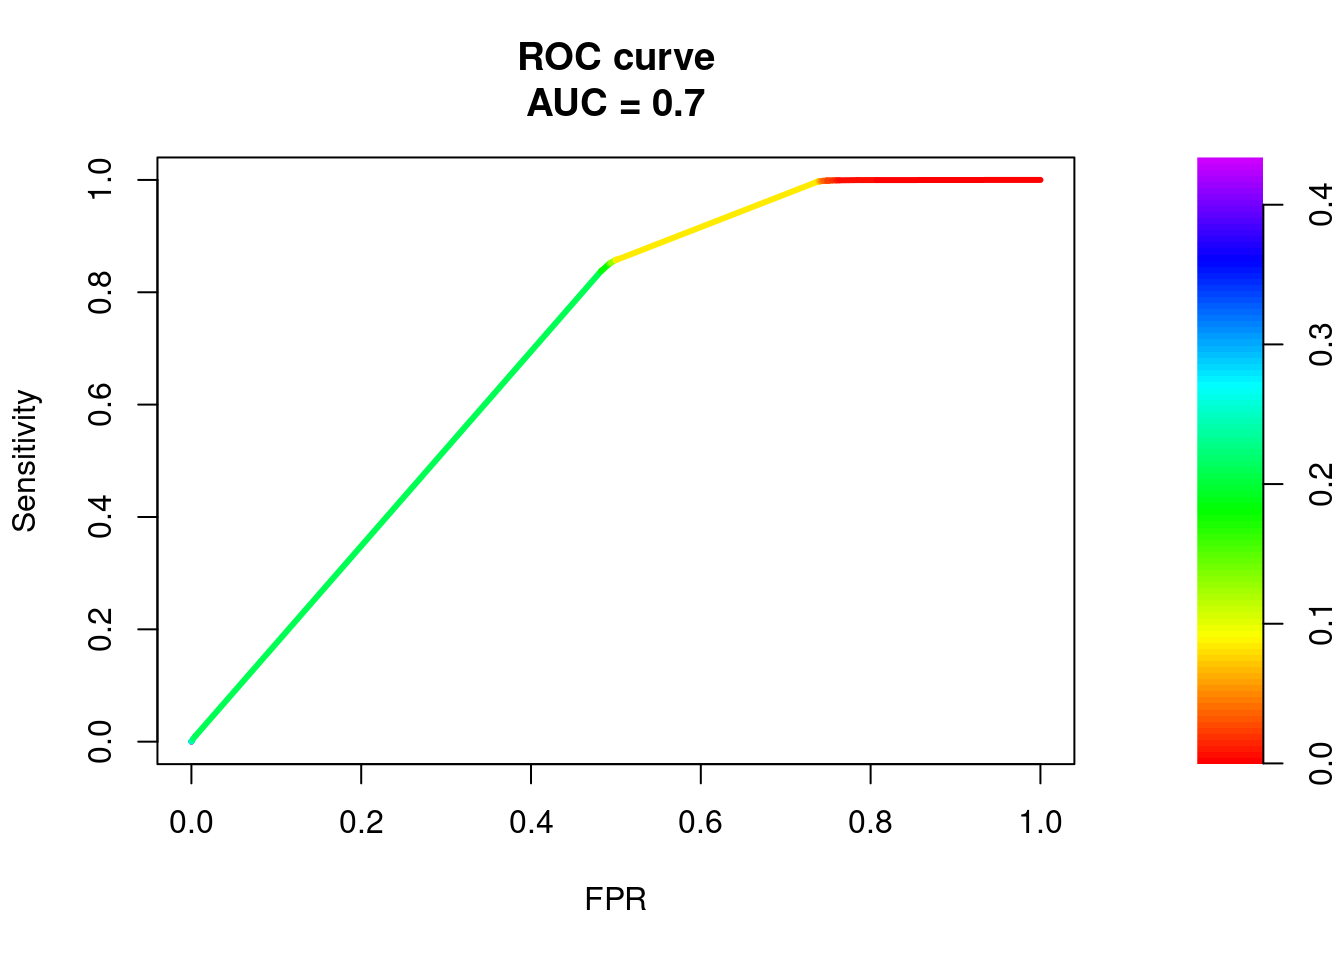
\includegraphics{bigdata_files/figure-latex/unnamed-chunk-12-1.pdf}

Hence, econometrics techniques such as the lasso help deal with \emph{big P} problems by providing reasonable ways to select a good predictive model (in other words, decide which of the many variables should be included).

\hypertarget{a-practical-big-n-problem}{%
\section{\texorpdfstring{A practical \emph{big N} problem}{A practical big N problem}}\label{a-practical-big-n-problem}}

Big N problems are situations in which we know what type of model we want to use but the \emph{number of observations} is too big to run the estimation (the computer crashes or slows down significantly). The simplest statistical solution to such a problem is usually to just estimate the model based on a smaller sample. However, we might not want to do that for other reasons (see introduction above). As an illustration of how an alternative statistical procedure can speed up the analysis of big N datasets, we look at a procedure to estimate linear models when the classical OLS estimator is computationally too demanding when analyzing large datasets: The \emph{Uluru} algorithm \citep{dhillon_2013}.

\hypertarget{ols-as-a-point-of-reference}{%
\subsection{OLS as a point of reference}\label{ols-as-a-point-of-reference}}

Recall the OLS estimator in matrix notation, given the linear model \(\mathbf{y}=\mathbf{X}\beta + \epsilon\):

\(\hat{\beta}_{OLS} = (\mathbf{X}^\intercal\mathbf{X})^{-1}\mathbf{X}^{\intercal}\mathbf{y}\).

In order to compute \(\hat{\beta}_{OLS}\), we have to compute \((\mathbf{X}^\intercal\mathbf{X})^{-1}\), which implies a computationally expensive matrix inversion.\footnote{The computational complexity of this is larger than \(O(n^{2})\). That is, for an input of size \(n\), the time needed to compute (or the number of operations needed) is \(n^2\).} If our dataset is large, \(\mathbf{X}\) is large and the inversion can take up a lot of computation time. Moreover, the inversion and matrix multiplication to get \(\hat{\beta}_{OLS}\) needs a lot of memory. In practice, it might well be that the estimation of a linear model via OLS with the standard approach in R (\texttt{lm()}) brings a computer to its knees, as there is not enough RAM available.

To further illustrate the point, we implement the OLS estimator in R.

\begin{Shaded}
\begin{Highlighting}[]
\NormalTok{beta\_ols }\OtherTok{\textless{}{-}} 
     \ControlFlowTok{function}\NormalTok{(X, y) \{}
          
          \CommentTok{\# compute cross products and inverse}
\NormalTok{          XXi }\OtherTok{\textless{}{-}} \FunctionTok{solve}\NormalTok{(}\FunctionTok{crossprod}\NormalTok{(X,X))}
\NormalTok{          Xy }\OtherTok{\textless{}{-}} \FunctionTok{crossprod}\NormalTok{(X, y) }
          
          \FunctionTok{return}\NormalTok{( XXi  }\SpecialCharTok{\%*\%}\NormalTok{ Xy )}
\NormalTok{     \}}
\end{Highlighting}
\end{Shaded}

Now, we will test our OLS estimator function with a few (pseudo-)random numbers in a Monte Carlo study. First, we set the sample size parameters \texttt{n} (the number of observations in our pseudo-sample) and \texttt{p} (the number of variables describing each of these observations) and initiate the dataset \texttt{X}.

\begin{Shaded}
\begin{Highlighting}[]
\CommentTok{\# set parameter values}
\NormalTok{n }\OtherTok{\textless{}{-}} \DecValTok{10000000}
\NormalTok{p }\OtherTok{\textless{}{-}} \DecValTok{4} 

\CommentTok{\# generate sample based on Monte Carlo}
\CommentTok{\# generate a design matrix (\textasciitilde{} our \textquotesingle{}dataset\textquotesingle{}) }
\CommentTok{\# with 4 variables and 10,000 observations}
\NormalTok{X }\OtherTok{\textless{}{-}} \FunctionTok{matrix}\NormalTok{(}\FunctionTok{rnorm}\NormalTok{(n}\SpecialCharTok{*}\NormalTok{p, }\AttributeTok{mean =} \DecValTok{10}\NormalTok{), }\AttributeTok{ncol =}\NormalTok{ p)}
\CommentTok{\# add column for intercept}
\NormalTok{X }\OtherTok{\textless{}{-}} \FunctionTok{cbind}\NormalTok{(}\FunctionTok{rep}\NormalTok{(}\DecValTok{1}\NormalTok{, n), X)}
\end{Highlighting}
\end{Shaded}

Now we define what the real linear model that we have in mind looks like and compute the output \texttt{y} of this model, given the input \texttt{X}.\footnote{In reality we would not know this, of course. Acting as if we knew the real model is exactly the point of Monte Carlo studies. It allows us to analyze the properties of estimators by simulation.}

\begin{Shaded}
\begin{Highlighting}[]
\CommentTok{\# MC model}
\NormalTok{y }\OtherTok{\textless{}{-}} \DecValTok{2} \SpecialCharTok{+} \FloatTok{1.5}\SpecialCharTok{*}\NormalTok{X[,}\DecValTok{2}\NormalTok{] }\SpecialCharTok{+} \DecValTok{4}\SpecialCharTok{*}\NormalTok{X[,}\DecValTok{3}\NormalTok{] }\SpecialCharTok{{-}} \FloatTok{3.5}\SpecialCharTok{*}\NormalTok{X[,}\DecValTok{4}\NormalTok{] }\SpecialCharTok{+} \FloatTok{0.5}\SpecialCharTok{*}\NormalTok{X[,}\DecValTok{5}\NormalTok{] }\SpecialCharTok{+} \FunctionTok{rnorm}\NormalTok{(n)}
\end{Highlighting}
\end{Shaded}

Finally, we test our \texttt{beta\_ols} function.

\begin{Shaded}
\begin{Highlighting}[]
\CommentTok{\# apply the OLS estimator}
\FunctionTok{beta\_ols}\NormalTok{(X, y)}
\end{Highlighting}
\end{Shaded}

\begin{verbatim}
##        [,1]
## [1,]  1.992
## [2,]  1.500
## [3,]  4.001
## [4,] -3.500
## [5,]  0.500
\end{verbatim}

\hypertarget{the-uluru-algorithm-as-an-alternative-to-ols}{%
\subsection{\texorpdfstring{The \emph{Uluru} algorithm as an alternative to OLS}{The Uluru algorithm as an alternative to OLS}}\label{the-uluru-algorithm-as-an-alternative-to-ols}}

Following \citet{dhillon_2013}, we implement a procedure to compute \(\hat{\beta}_{Uluru}\):

\[\hat{\beta}_{Uluru}=\hat{\beta}_{FS} + \hat{\beta}_{correct}\], where
\[\hat{\beta}_{FS} = (\mathbf{X}_{subs}^\intercal\mathbf{X}_{subs})^{-1}\mathbf{X}_{subs}^{\intercal}\mathbf{y}_{subs}\], and
\[\hat{\beta}_{correct}= \frac{n_{subs}}{n_{rem}} \cdot (\mathbf{X}_{subs}^\intercal\mathbf{X}_{subs})^{-1} \mathbf{X}_{rem}^{\intercal}\mathbf{R}_{rem}\], and
\[\mathbf{R}_{rem} = \mathbf{Y}_{rem} - \mathbf{X}_{rem}  \cdot \hat{\beta}_{FS}\].

The key idea behind this is that the computational bottleneck of the OLS estimator, the cross product and matrix inversion,\((\mathbf{X}^\intercal\mathbf{X})^{-1}\), is only computed on a sub-sample (\(X_{subs}\), etc.), not the entire dataset. However, the remainder of the dataset is also taken into consideration (in order to correct a bias arising from the sub-sampling). Again, we implement the estimator in R to further illustrate this point.

\begin{Shaded}
\begin{Highlighting}[]
\NormalTok{beta\_uluru }\OtherTok{\textless{}{-}}
     \ControlFlowTok{function}\NormalTok{(X\_subs, y\_subs, X\_rem, y\_rem) \{}
          
          \CommentTok{\# compute beta\_fs }
          \CommentTok{\#(this is simply OLS applied to the subsample)}
\NormalTok{          XXi\_subs }\OtherTok{\textless{}{-}} \FunctionTok{solve}\NormalTok{(}\FunctionTok{crossprod}\NormalTok{(X\_subs, X\_subs))}
\NormalTok{          Xy\_subs }\OtherTok{\textless{}{-}} \FunctionTok{crossprod}\NormalTok{(X\_subs, y\_subs)}
\NormalTok{          b\_fs }\OtherTok{\textless{}{-}}\NormalTok{ XXi\_subs  }\SpecialCharTok{\%*\%}\NormalTok{ Xy\_subs}
          
          \CommentTok{\# compute \textbackslash{}mathbf\{R\}\_\{rem\}}
\NormalTok{          R\_rem }\OtherTok{\textless{}{-}}\NormalTok{ y\_rem }\SpecialCharTok{{-}}\NormalTok{ X\_rem }\SpecialCharTok{\%*\%}\NormalTok{ b\_fs}
          
          \CommentTok{\# compute \textbackslash{}hat\{\textbackslash{}beta\}\_\{correct\}}
\NormalTok{          b\_correct }\OtherTok{\textless{}{-}} 
\NormalTok{               (}\FunctionTok{nrow}\NormalTok{(X\_subs)}\SpecialCharTok{/}\NormalTok{(}\FunctionTok{nrow}\NormalTok{(X\_rem))) }\SpecialCharTok{*}
\NormalTok{               XXi\_subs }\SpecialCharTok{\%*\%} \FunctionTok{crossprod}\NormalTok{(X\_rem, R\_rem)}

          \CommentTok{\# beta uluru       }
          \FunctionTok{return}\NormalTok{(b\_fs }\SpecialCharTok{+}\NormalTok{ b\_correct)}
\NormalTok{     \}}
\end{Highlighting}
\end{Shaded}

We then test it with the same input as above:

\begin{Shaded}
\begin{Highlighting}[]
\CommentTok{\# set size of sub{-}sample}
\NormalTok{n\_subs }\OtherTok{\textless{}{-}} \DecValTok{1000}
\CommentTok{\# select sub{-}sample and remainder}
\NormalTok{n\_obs }\OtherTok{\textless{}{-}} \FunctionTok{nrow}\NormalTok{(X)}
\NormalTok{X\_subs }\OtherTok{\textless{}{-}}\NormalTok{ X[1L}\SpecialCharTok{:}\NormalTok{n\_subs,]}
\NormalTok{y\_subs }\OtherTok{\textless{}{-}}\NormalTok{ y[1L}\SpecialCharTok{:}\NormalTok{n\_subs]}
\NormalTok{X\_rem }\OtherTok{\textless{}{-}}\NormalTok{ X[(n\_subs}\SpecialCharTok{+}\NormalTok{1L)}\SpecialCharTok{:}\NormalTok{n\_obs,]}
\NormalTok{y\_rem }\OtherTok{\textless{}{-}}\NormalTok{ y[(n\_subs}\SpecialCharTok{+}\NormalTok{1L)}\SpecialCharTok{:}\NormalTok{n\_obs]}

\CommentTok{\# apply the uluru estimator}
\FunctionTok{beta\_uluru}\NormalTok{(X\_subs, y\_subs, X\_rem, y\_rem)}
\end{Highlighting}
\end{Shaded}

\begin{verbatim}
##        [,1]
## [1,]  2.188
## [2,]  1.489
## [3,]  3.998
## [4,] -3.503
## [5,]  0.498
\end{verbatim}

This looks quite good already. Let's have a closer look with a little Monte Carlo study. The aim of the simulation study is to visualize the difference between the classical OLS approach and the \emph{Uluru} algorithm with regard to bias and time complexity if we increase the sub-sample size in \emph{Uluru}. For simplicity, we only look at the first estimated coefficient \(\beta_{1}\).

\begin{Shaded}
\begin{Highlighting}[]
\CommentTok{\# define sub{-}samples}
\NormalTok{n\_subs\_sizes }\OtherTok{\textless{}{-}} \FunctionTok{seq}\NormalTok{(}\AttributeTok{from =} \DecValTok{1000}\NormalTok{, }\AttributeTok{to =} \DecValTok{500000}\NormalTok{, }\AttributeTok{by=}\DecValTok{10000}\NormalTok{)}
\NormalTok{n\_runs }\OtherTok{\textless{}{-}} \FunctionTok{length}\NormalTok{(n\_subs\_sizes)}
\CommentTok{\# compute uluru result, stop time}
\NormalTok{mc\_results }\OtherTok{\textless{}{-}} \FunctionTok{rep}\NormalTok{(}\ConstantTok{NA}\NormalTok{, n\_runs)}
\NormalTok{mc\_times }\OtherTok{\textless{}{-}} \FunctionTok{rep}\NormalTok{(}\ConstantTok{NA}\NormalTok{, n\_runs)}
\ControlFlowTok{for}\NormalTok{ (i }\ControlFlowTok{in} \DecValTok{1}\SpecialCharTok{:}\NormalTok{n\_runs) \{}
     \CommentTok{\# set size of sub{-}sample}
\NormalTok{     n\_subs }\OtherTok{\textless{}{-}}\NormalTok{ n\_subs\_sizes[i]}
     \CommentTok{\# select sub{-}sample and remainder}
\NormalTok{     n\_obs }\OtherTok{\textless{}{-}} \FunctionTok{nrow}\NormalTok{(X)}
\NormalTok{     X\_subs }\OtherTok{\textless{}{-}}\NormalTok{ X[1L}\SpecialCharTok{:}\NormalTok{n\_subs,]}
\NormalTok{     y\_subs }\OtherTok{\textless{}{-}}\NormalTok{ y[1L}\SpecialCharTok{:}\NormalTok{n\_subs]}
\NormalTok{     X\_rem }\OtherTok{\textless{}{-}}\NormalTok{ X[(n\_subs}\SpecialCharTok{+}\NormalTok{1L)}\SpecialCharTok{:}\NormalTok{n\_obs,]}
\NormalTok{     y\_rem }\OtherTok{\textless{}{-}}\NormalTok{ y[(n\_subs}\SpecialCharTok{+}\NormalTok{1L)}\SpecialCharTok{:}\NormalTok{n\_obs]}
     
\NormalTok{     mc\_results[i] }\OtherTok{\textless{}{-}} \FunctionTok{beta\_uluru}\NormalTok{(X\_subs,}
\NormalTok{                                 y\_subs,}
\NormalTok{                                 X\_rem,}
\NormalTok{                                 y\_rem)[}\DecValTok{2}\NormalTok{] }\CommentTok{\# (1 is the intercept)}
\NormalTok{     mc\_times[i] }\OtherTok{\textless{}{-}} \FunctionTok{system.time}\NormalTok{(}\FunctionTok{beta\_uluru}\NormalTok{(X\_subs,}
\NormalTok{                                           y\_subs,}
\NormalTok{                                           X\_rem,}
\NormalTok{                                           y\_rem))[}\DecValTok{3}\NormalTok{]}
     
\NormalTok{\}}

\CommentTok{\# compute OLS results and OLS time}
\NormalTok{ols\_time }\OtherTok{\textless{}{-}} \FunctionTok{system.time}\NormalTok{(}\FunctionTok{beta\_ols}\NormalTok{(X, y))}
\NormalTok{ols\_res }\OtherTok{\textless{}{-}} \FunctionTok{beta\_ols}\NormalTok{(X, y)[}\DecValTok{2}\NormalTok{]}
\end{Highlighting}
\end{Shaded}

Let's visualize the comparison with OLS.

\begin{Shaded}
\begin{Highlighting}[]
\CommentTok{\# load packages}
\FunctionTok{library}\NormalTok{(ggplot2)}

\CommentTok{\# prepare data to plot}
\NormalTok{plotdata }\OtherTok{\textless{}{-}} \FunctionTok{data.frame}\NormalTok{(}\AttributeTok{beta1 =}\NormalTok{ mc\_results,}
                       \AttributeTok{time\_elapsed =}\NormalTok{ mc\_times,}
                       \AttributeTok{subs\_size =}\NormalTok{ n\_subs\_sizes)}
\end{Highlighting}
\end{Shaded}

First, let's look at the time used estimate the linear model.

\begin{Shaded}
\begin{Highlighting}[]
\FunctionTok{ggplot}\NormalTok{(plotdata, }\FunctionTok{aes}\NormalTok{(}\AttributeTok{x =}\NormalTok{ subs\_size, }\AttributeTok{y =}\NormalTok{ time\_elapsed)) }\SpecialCharTok{+}
     \FunctionTok{geom\_point}\NormalTok{(}\AttributeTok{color=}\StringTok{"darkgreen"}\NormalTok{) }\SpecialCharTok{+} 
     \FunctionTok{geom\_hline}\NormalTok{(}\AttributeTok{yintercept =}\NormalTok{ ols\_time[}\DecValTok{3}\NormalTok{],}
                \AttributeTok{color =} \StringTok{"red"}\NormalTok{, }
                \AttributeTok{size =} \DecValTok{1}\NormalTok{) }\SpecialCharTok{+}
     \FunctionTok{theme\_minimal}\NormalTok{() }\SpecialCharTok{+}
     \FunctionTok{ylab}\NormalTok{(}\StringTok{"Time elapsed"}\NormalTok{) }\SpecialCharTok{+}
     \FunctionTok{xlab}\NormalTok{(}\StringTok{"Subsample size"}\NormalTok{)}
\end{Highlighting}
\end{Shaded}

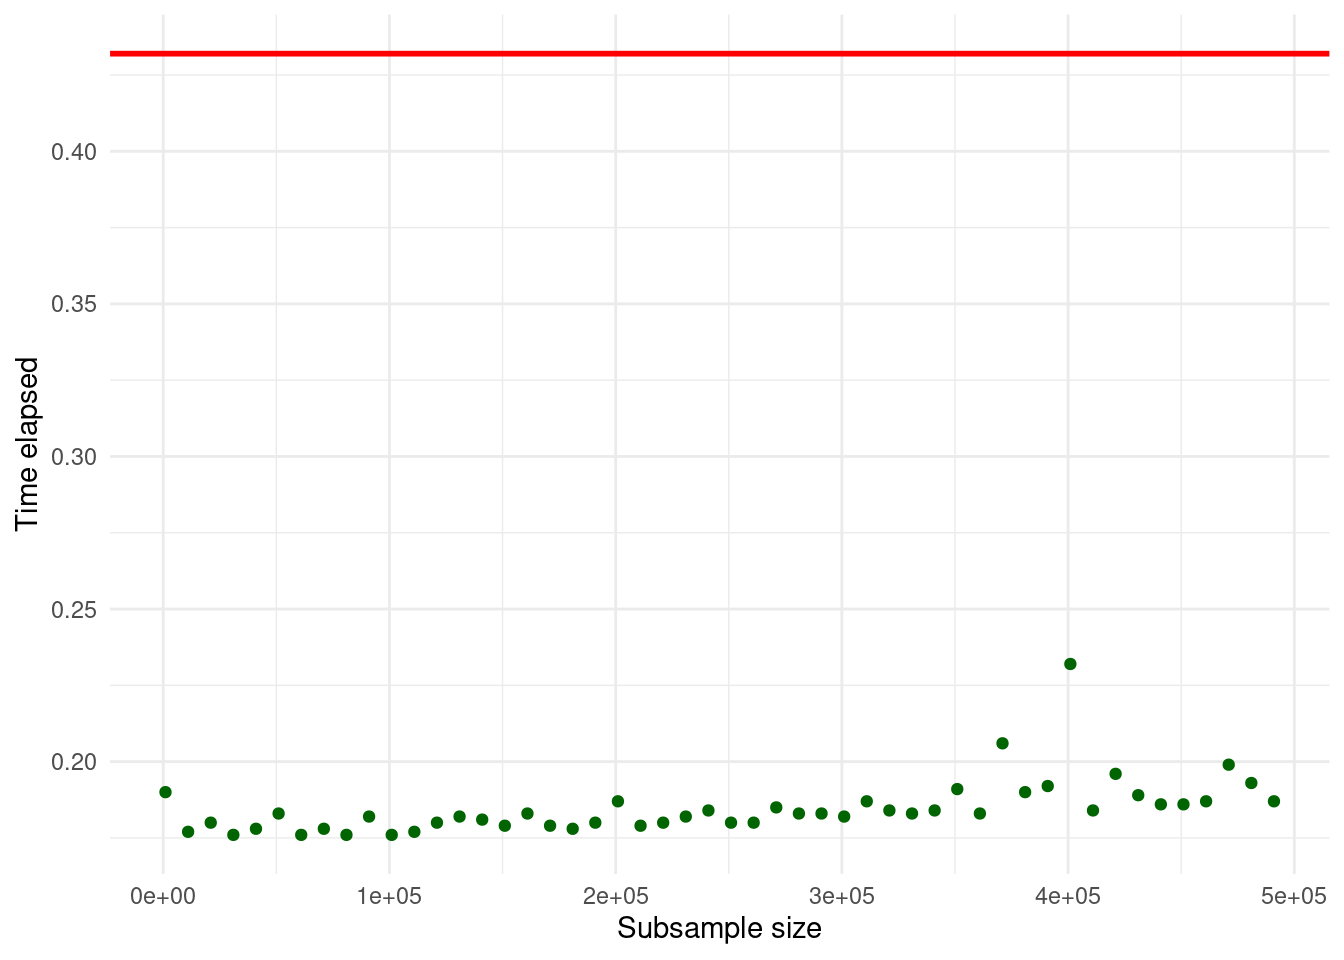
\includegraphics{bigdata_files/figure-latex/unnamed-chunk-21-1.pdf}

The horizontal red line indicates the computation time for estimation via OLS; the green points indicate the computation time for the estimation via the \emph{Ulruru} algorithm. Note that even for large sub-samples, the computation time is substantially lower than for OLS.

Finally, let's have a look at how close the results are to OLS.

\begin{Shaded}
\begin{Highlighting}[]
\FunctionTok{ggplot}\NormalTok{(plotdata, }\FunctionTok{aes}\NormalTok{(}\AttributeTok{x =}\NormalTok{ subs\_size, }\AttributeTok{y =}\NormalTok{ beta1)) }\SpecialCharTok{+}
     \FunctionTok{geom\_hline}\NormalTok{(}\AttributeTok{yintercept =}\NormalTok{ ols\_res,}
                \AttributeTok{color =} \StringTok{"red"}\NormalTok{, }
                \AttributeTok{size =} \DecValTok{1}\NormalTok{) }\SpecialCharTok{+}
       \FunctionTok{geom\_hline}\NormalTok{(}\AttributeTok{yintercept =} \FloatTok{1.5}\NormalTok{,}
                \AttributeTok{color =} \StringTok{"green"}\NormalTok{,}
                \AttributeTok{size =} \DecValTok{1}\NormalTok{) }\SpecialCharTok{+}
     \FunctionTok{geom\_point}\NormalTok{(}\AttributeTok{color=}\StringTok{"darkgreen"}\NormalTok{) }\SpecialCharTok{+} 

     \FunctionTok{theme\_minimal}\NormalTok{() }\SpecialCharTok{+}
     \FunctionTok{ylab}\NormalTok{(}\StringTok{"Estimated coefficient"}\NormalTok{) }\SpecialCharTok{+}
     \FunctionTok{xlab}\NormalTok{(}\StringTok{"Subsample size"}\NormalTok{)}
\end{Highlighting}
\end{Shaded}

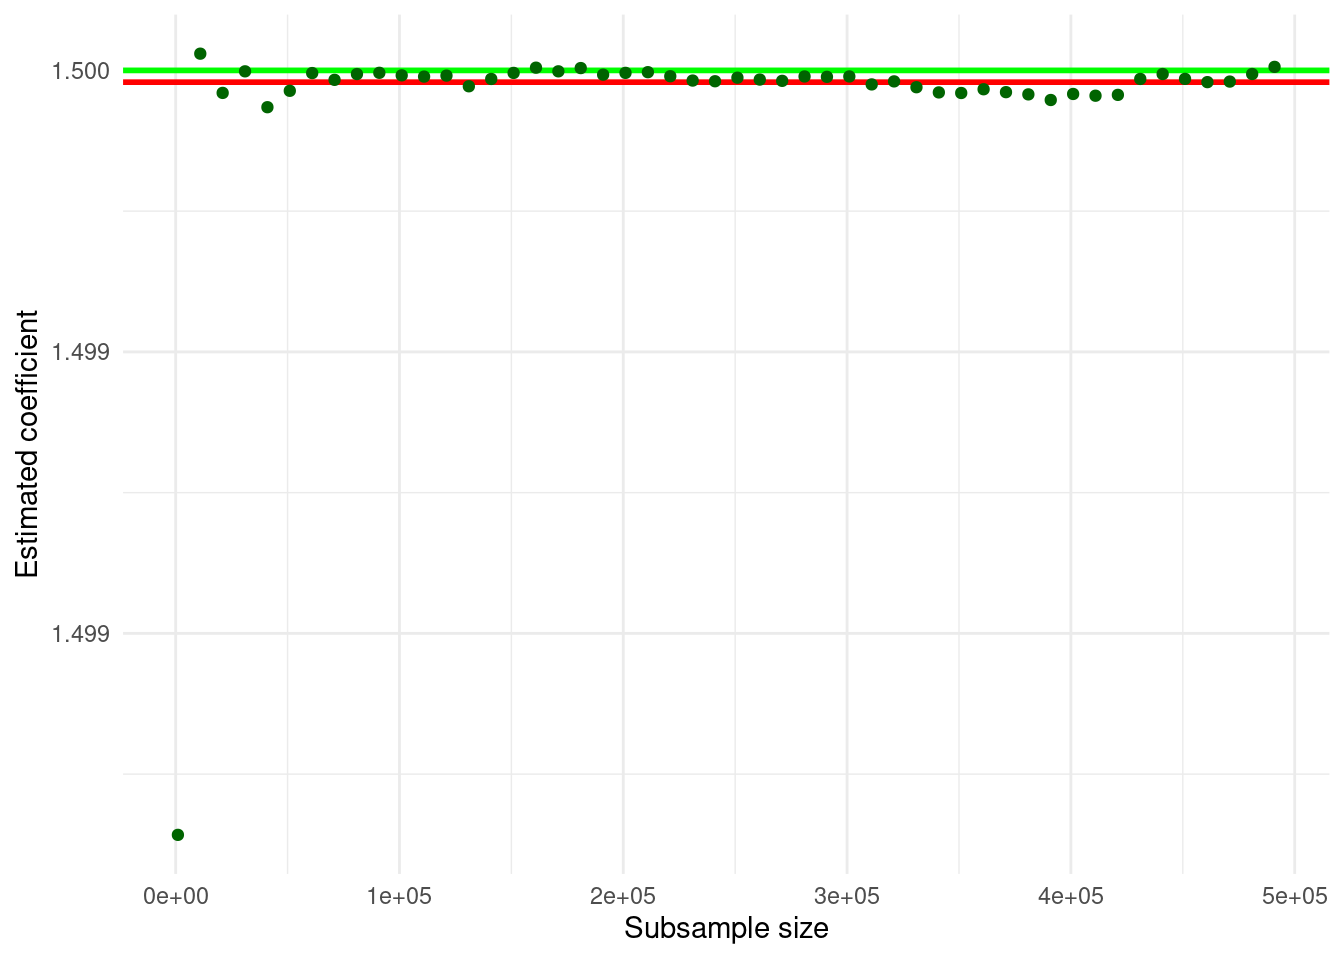
\includegraphics{bigdata_files/figure-latex/unnamed-chunk-22-1.pdf}

The horizontal red line indicates the size of the estimated coefficient, when using OLS. The horizontal green line indicates the size of the actual coefficient. The green points indicate the size of the same coefficient estimated by the \emph{Uluru} algorithm for different sub-sample sizes. Note that even relatively small sub-samples already deliver estimates very close to the OLS estimates.

Taken together, the example illustrates that alternative statistical methods, optimized for large amounts of data, can deliver results very close to traditional approaches. Yet, they can deliver these results much more efficiently.

\hypertarget{conclusion}{%
\section{Conclusion}\label{conclusion}}

When applying econometrics to `'large'' datasets, two types of problems dominate: a) the number of covariates is `too large' to handle with traditional estimators (\emph{big P} problem) and/or b) the number of observations is `too large' to handle with traditional estimators (\emph{big N} problem). The first problem is being addressed by an interesting new strain of econometrics literature, which builds on previously known machine learning algorithms such as lasso and random forest and clarifies the statistical properties of predictions coming from these algorithms. While the following chapters will repeatedly link to these contributions in specific code examples, the main focus of the following chapters lies on the \emph{big N} problem and the key underlying concepts (in terms of software, hardware, and faster new estimators) to productively perform data analytics tasks when confronted with large amounts of data. Several of the following chapters will also focus on something that is often ignored in the applied econometrics literature: how do we get from the raw data to the cleaned and filtered analytic dataset to run regressions. While these topics are generally highly relevant for proper data science and data analytics workflows, you will see that these topics are absolutely crucial when working with large datasets.

\hypertarget{part-platform-software-and-computing-resources}{%
\part{Platform: Software and Computing Resources}\label{part-platform-software-and-computing-resources}}

\hypertarget{software-programming-with-big-data}{%
\chapter{Software: Programming with (Big) Data}\label{software-programming-with-big-data}}

The programming language and computing environment \emph{R} is particularly made for writing code in a data analytics context. However, the language was developed at a time when data analytics was primarily focused on moderately sized data sets that can easily be loaded/imported and worked with on a common PC. Depending on the field or industry you work in, this is not anymore the case today. In this chapter, we will explore some of R's (potential) weaknesses as well as learn how to avoid them and how to exploit some of R's strengths when it comes to working with large data sets. The first part of this chapter is primarily focused on understanding code profiling and improving code with the aim of making computationally intense data analytics scripts in R run faster. This chapter presupposes basic knowledge of R data structures and data types as well as experience with basic programming concepts such as loops.\footnote{Appendix B reviews the most relevant concepts regarding data types and data structures in R.}

While R is a very useful tool for many aspects of big data analytics that we will cover in the following chapters, R alone is not enough for a basic big data analytics toolbox. The second part of this chapter introduces the reader to the \emph{Structured Query Language (SQL)}, a programming language designed for managing data in relational databases. Although the type of databases where SQL is traditionally encountered would not necessarily be considered part of big data analytics today, some versions of SQL are now used with systems particularly designed for big data analytics (such as Amazon Athena and Google BigQuery). Hence, with a good knowledge of R in combination with basic SQL skills, you will be able to productively engage with a large array of practical big data analytics problems.

\hypertarget{domains-of-programming-with-big-data}{%
\section{Domains of programming with (big) data}\label{domains-of-programming-with-big-data}}

Programming tasks in the context of data analytics typically fall into one of the following broad categories.

\begin{itemize}
\tightlist
\item
  Procedures to import/export data.
\item
  Procedures to clean and filter data.
\item
  Implement functions for statistical analysis.
\end{itemize}

When writing a program to process large amounts of data in any of these areas, it is helpful to take into consideration the following design choices:

\begin{enumerate}
\def\labelenumi{\arabic{enumi}.}
\tightlist
\item
  Which basic (already implemented) R functions are more or less suitable as building blocks for the program?\footnote{Throughout the rest of this book, I will point to specialized R packages and functions that are particularly designed to work with large amounts of data. Where necessary, we will also look more closely at the underlying concepts that explain why these specialized packages work better with large amounts of data than the standard approaches.}
\item
  How can we exploit/avoid some of R's lower-level characteristics in order to write more efficient code?
\item
  Is there a need to interface with a lower-level programming language in order to speed up the code? (advanced topic)
\end{enumerate}

Finally, there is an additional important point to be made regarding the writing of code for \emph{statistical analysis}: Independent of \emph{how} we write a statistical procedure in R (or in any other language, for that matter), keep in mind that there might be an \emph{alternative statistical procedure/algorithm} that is faster but delivers approximately the same result (as long as we use a sufficiently large sample).

\hypertarget{measuring-r-performance}{%
\section{Measuring R performance}\label{measuring-r-performance}}

When writing a data analysis script in R to process large amounts of data, it generally makes sense to first test each crucial part of the script with a small sub-sample. In order to nevertheless quickly recognize potential bottle necks, there are a couple of R packages that help you keep track of how long exactly each component of your script needs to process as well as how much memory it uses. The table below lists some of the packages and functions that you should keep in mind when \emph{``profiling''} and testing your code.

\begin{longtable}[]{@{}
  >{\raggedright\arraybackslash}p{(\columnwidth - 4\tabcolsep) * \real{0.1270}}
  >{\raggedright\arraybackslash}p{(\columnwidth - 4\tabcolsep) * \real{0.1587}}
  >{\raggedright\arraybackslash}p{(\columnwidth - 4\tabcolsep) * \real{0.7143}}@{}}
\toprule
\begin{minipage}[b]{\linewidth}\raggedright
package
\end{minipage} & \begin{minipage}[b]{\linewidth}\raggedright
function
\end{minipage} & \begin{minipage}[b]{\linewidth}\raggedright
purpose
\end{minipage} \\
\midrule
\endhead
\texttt{utils} & \texttt{object.size()} & Provides an estimate of the memory that is being used to store an R object. \\
\texttt{pryr} & \texttt{object\_size()} & Works similarly to \texttt{object.size()}, but counts more accurately and includes the size of environments. \\
\texttt{pryr} & \texttt{mem\_used()} & Returns the total amount of memory (in megabytes) currently used by R. \\
\texttt{pryr} & \texttt{mem\_change()} & Shows the change in memory (in megabytes) before and after running code. \\
\texttt{base} & \texttt{system.time()} & Returns CPU (and other) times that an R expression used. \\
\texttt{microbenchmark} & \texttt{microbenchmark()} & Highly accurate timing of R expression evaluation. \\
\texttt{bench} & \texttt{mark()} & Benchmark a series of functions. \\
\texttt{profvis} & \texttt{profvis()} & Profiles an R expression and visualizes the profiling data (usage of memory, time elapsed, etc.). \\
\bottomrule
\end{longtable}

Most of these functions are used in an interactive way in the R console. They serve either of two purposes that are central to profiling and improving your code's performance. First, in order to assess the performance of your R code you probably want to know how long it takes to run your entire script or a specific part of your script. The \texttt{system.time()}-function provides an easy way to check this. This function is loaded by default with R, there is no need to install an additional package. Simply wrap it around the line(s) of code that you want to assess.

\begin{Shaded}
\begin{Highlighting}[]
\CommentTok{\# how much time does it take to run this loop?}
\FunctionTok{system.time}\NormalTok{(}\ControlFlowTok{for}\NormalTok{ (i }\ControlFlowTok{in} \DecValTok{1}\SpecialCharTok{:}\DecValTok{100}\NormalTok{) \{i }\SpecialCharTok{+} \DecValTok{5}\NormalTok{\})}
\end{Highlighting}
\end{Shaded}

\begin{verbatim}
##    user  system elapsed 
##   0.002   0.000   0.002
\end{verbatim}

Note that each time you run this line of code, the returned amount of time varies slightly. This has to do with the fact that the actual time needed to run a line of code can depend on various other processes happening at the same time on your computer.

The \texttt{microbenchmark} and \texttt{bench} packages provide additional functions to measure execution time in more sophisticated ways. In particular, they account for the fact that the processing time for the same code might vary and automatically run the code several times in order to return statistics about the processing time. In addition, \texttt{microbenchmark()} provides highly detailed and highly accurate timing of R expression evaluation. The function is particularly useful to accurately find even ``minor'' room for improvement when testing a data analysis script on a smaller sub-sample (which might scale when working on a large data set). For example, suppose you need to run a for-loop over millions of iterations and there are different ways to implement the loop of the body (which does not take too much time to process in one iteration). Note that the function actually evaluates the R expression in question many times and returns a statistical summary of the timings.

\begin{Shaded}
\begin{Highlighting}[]
\CommentTok{\# load package}
\FunctionTok{library}\NormalTok{(microbenchmark)}
\CommentTok{\# how much time does it take to run this loop (exactly)?}
\FunctionTok{microbenchmark}\NormalTok{(}\ControlFlowTok{for}\NormalTok{ (i }\ControlFlowTok{in} \DecValTok{1}\SpecialCharTok{:}\DecValTok{100}\NormalTok{) \{i }\SpecialCharTok{+} \DecValTok{5}\NormalTok{\})}
\end{Highlighting}
\end{Shaded}

\begin{verbatim}
## Unit: milliseconds
##                            expr   min    lq mean
##  for (i in 1:100) {     i + 5 } 1.129 1.228 1.36
##  median   uq   max neval
##   1.278 1.35 4.859   100
\end{verbatim}

Second, a key aspect to improving the performance of data analysis scripts in R is to detect inefficient memory allocation as well as avoiding that an R-object is either growing too much or is generally too large to handle in memory. To this end, you might want to monitor how much memory R occupies at different points in your script as well as how much memory is taken up by individual R objects. For example, \texttt{object.size()} returns the size of an R object, that is the amount of memory it takes up in the R environment in bytes (\texttt{pryr::object\_size()} counts slightly more accurately).

\begin{Shaded}
\begin{Highlighting}[]
\NormalTok{hello }\OtherTok{\textless{}{-}} \StringTok{"Hello, World!"}
\FunctionTok{object.size}\NormalTok{(hello)}
\end{Highlighting}
\end{Shaded}

\begin{verbatim}
## 120 bytes
\end{verbatim}

This is useful to implementing your script with a generally less memory-intense approach. For example, for a specific task it might not matter whether a particular variable is stored as a \texttt{character} vector or a \texttt{factor}. But storing it as \texttt{character} turns out to be more memory intense (why?).

\begin{Shaded}
\begin{Highlighting}[]
\CommentTok{\# initiate a large string vector containing letters}
\NormalTok{large\_string }\OtherTok{\textless{}{-}} \FunctionTok{rep}\NormalTok{(LETTERS[}\DecValTok{1}\SpecialCharTok{:}\DecValTok{20}\NormalTok{], }\DecValTok{1000}\SpecialCharTok{\^{}}\DecValTok{2}\NormalTok{)}
\FunctionTok{head}\NormalTok{(large\_string)}
\end{Highlighting}
\end{Shaded}

\begin{verbatim}
## [1] "A" "B" "C" "D" "E" "F"
\end{verbatim}

\begin{Shaded}
\begin{Highlighting}[]
\CommentTok{\# store the same information as a factor in a new variable}
\NormalTok{large\_factor }\OtherTok{\textless{}{-}} \FunctionTok{as.factor}\NormalTok{(large\_string)}

\CommentTok{\# is one bigger than the other?}
\FunctionTok{object.size}\NormalTok{(large\_string) }\SpecialCharTok{{-}} \FunctionTok{object.size}\NormalTok{(large\_factor)}
\end{Highlighting}
\end{Shaded}

\begin{verbatim}
## 79999456 bytes
\end{verbatim}

\texttt{pryr::mem\_change()} is useful to track how different parts of your script affect the overall memory occupied by R.

\begin{Shaded}
\begin{Highlighting}[]
\CommentTok{\# load package}
\FunctionTok{library}\NormalTok{(pryr)}

\CommentTok{\# initiate a vector with 1000 (pseudo){-}random numbers}
\FunctionTok{mem\_change}\NormalTok{(}
\NormalTok{        thousand\_numbers }\OtherTok{\textless{}{-}} \FunctionTok{runif}\NormalTok{(}\DecValTok{1000}\NormalTok{)}
\NormalTok{        )}
\end{Highlighting}
\end{Shaded}

\begin{verbatim}
## 9.64 kB
\end{verbatim}

\begin{Shaded}
\begin{Highlighting}[]
\CommentTok{\# initiate a vector with 1M (pseudo){-}random numbers}
\FunctionTok{mem\_change}\NormalTok{(}
\NormalTok{        a\_million\_numbers }\OtherTok{\textless{}{-}} \FunctionTok{runif}\NormalTok{(}\DecValTok{1000}\SpecialCharTok{\^{}}\DecValTok{2}\NormalTok{)}
\NormalTok{        )}
\end{Highlighting}
\end{Shaded}

\begin{verbatim}
## 8 MB
\end{verbatim}

\texttt{bench::mark()} allows you to easily compare the performance of several different implementations of a code chunk both regarding timing and memory usage. The following code example illustrates this in a comparison of two approaches to computing the product of each element in a vector \texttt{x} with a factor \texttt{z}.

\begin{Shaded}
\begin{Highlighting}[]
\CommentTok{\# load packages}
\FunctionTok{library}\NormalTok{(bench)}

\CommentTok{\# initiate variables}
\NormalTok{x }\OtherTok{\textless{}{-}} \DecValTok{1}\SpecialCharTok{:}\DecValTok{10000}
\NormalTok{z }\OtherTok{\textless{}{-}} \FloatTok{1.5}
\CommentTok{\# approach 1: loop}
\NormalTok{multiplication }\OtherTok{\textless{}{-}} 
        \ControlFlowTok{function}\NormalTok{(x,z) \{}
\NormalTok{                result }\OtherTok{\textless{}{-}} \FunctionTok{c}\NormalTok{()}
                \ControlFlowTok{for}\NormalTok{ (i }\ControlFlowTok{in} \DecValTok{1}\SpecialCharTok{:}\FunctionTok{length}\NormalTok{(x)) \{result }\OtherTok{\textless{}{-}} \FunctionTok{c}\NormalTok{(result, x[i]}\SpecialCharTok{*}\NormalTok{z)\}}
                \FunctionTok{return}\NormalTok{(result)}
\NormalTok{        \}}
\NormalTok{result }\OtherTok{\textless{}{-}} \FunctionTok{multiplication}\NormalTok{(x,z)}
\FunctionTok{head}\NormalTok{(result)}
\end{Highlighting}
\end{Shaded}

\begin{verbatim}
## [1] 1.5 3.0 4.5 6.0 7.5 9.0
\end{verbatim}

\begin{Shaded}
\begin{Highlighting}[]
\CommentTok{\# approach II: "R{-}style"}
\NormalTok{result2 }\OtherTok{\textless{}{-}}\NormalTok{ x }\SpecialCharTok{*}\NormalTok{ z }
\FunctionTok{head}\NormalTok{(result2)}
\end{Highlighting}
\end{Shaded}

\begin{verbatim}
## [1] 1.5 3.0 4.5 6.0 7.5 9.0
\end{verbatim}

\begin{Shaded}
\begin{Highlighting}[]
\CommentTok{\# comparison}
\NormalTok{benchmarking }\OtherTok{\textless{}{-}} 
        \FunctionTok{mark}\NormalTok{(}
\NormalTok{        result }\OtherTok{\textless{}{-}} \FunctionTok{multiplication}\NormalTok{(x,z),}
\NormalTok{        result2 }\OtherTok{\textless{}{-}}\NormalTok{ x }\SpecialCharTok{*}\NormalTok{ z, }
        \AttributeTok{min\_iterations =} \DecValTok{50} 
\NormalTok{)}
\NormalTok{benchmarking[, }\DecValTok{4}\SpecialCharTok{:}\DecValTok{9}\NormalTok{]}
\end{Highlighting}
\end{Shaded}

\begin{verbatim}
## # A tibble: 2 x 3
##   `itr/sec` mem_alloc `gc/sec`
##       <dbl> <bch:byt>    <dbl>
## 1      13.1     382MB    11.2 
## 2   75944.     78.2KB     7.60
\end{verbatim}

In addition, the \texttt{bench} package provides a simple way to visualize these outputs:

\begin{Shaded}
\begin{Highlighting}[]
\FunctionTok{plot}\NormalTok{(benchmarking, }\AttributeTok{type =} \StringTok{"boxplot"}\NormalTok{)}
\end{Highlighting}
\end{Shaded}

\begin{verbatim}
## Loading required namespace: tidyr
\end{verbatim}

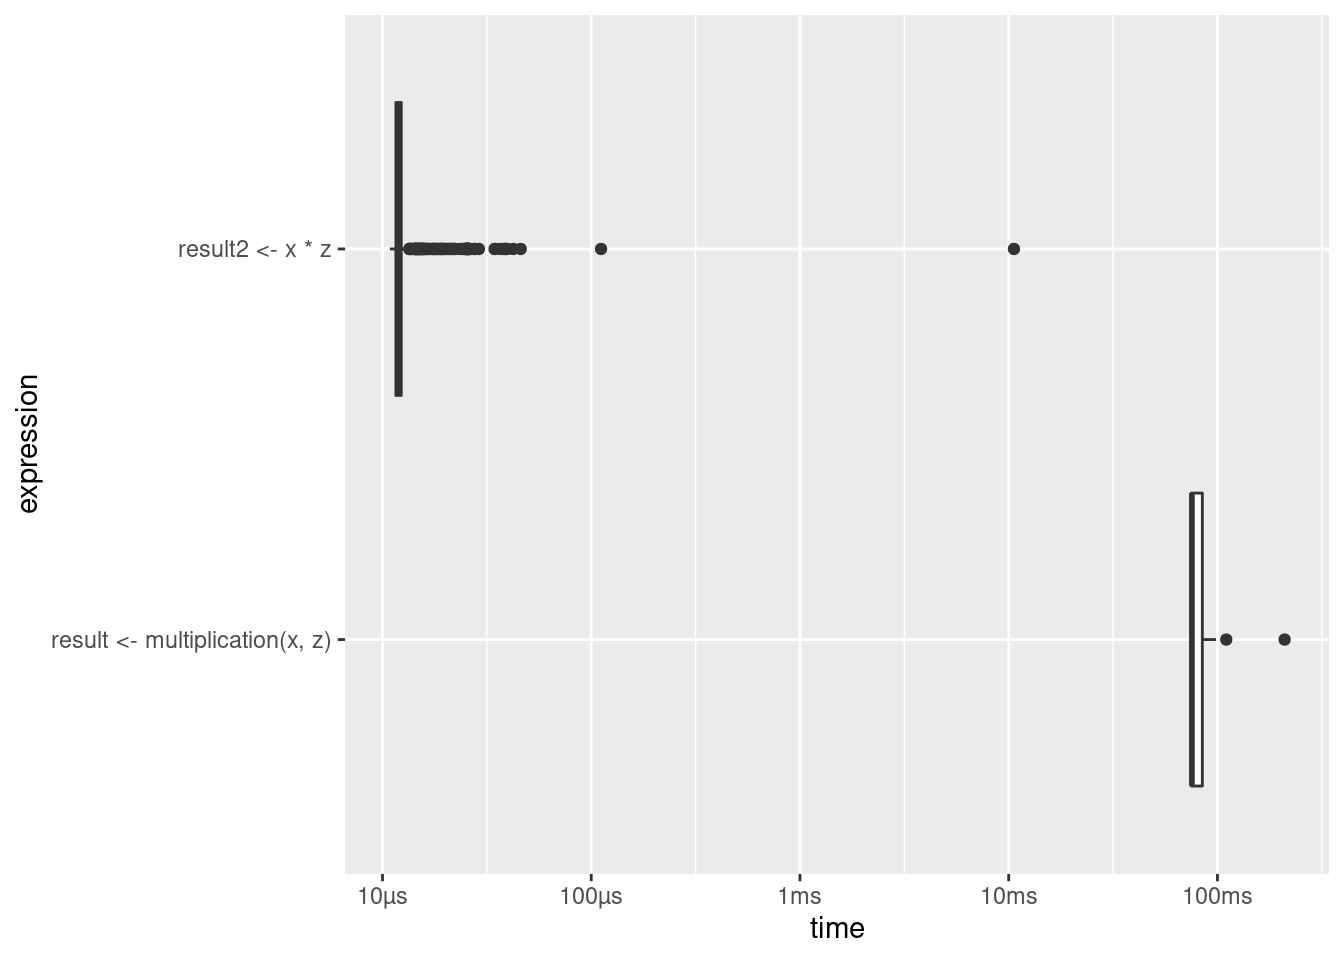
\includegraphics{bigdata_files/figure-latex/unnamed-chunk-30-1.pdf}

Finally, to analyze the performance of your entire script/program the \texttt{profvis} package provides visual summaries to quickly detect the most prominent bottle necks. You can either call this via the \texttt{profvis()} function with the code section to be profiled as argument, or via the RStudio user interface by clicking on the Code Tools menu in the editor window and select ``Profile selected lines''.

\begin{Shaded}
\begin{Highlighting}[]
\CommentTok{\# load package}
\FunctionTok{library}\NormalTok{(profvis)}

\CommentTok{\# analyse performance of several lines of code}
\FunctionTok{profvis}\NormalTok{(\{}
\NormalTok{        x }\OtherTok{\textless{}{-}} \DecValTok{1}\SpecialCharTok{:}\DecValTok{10000}
\NormalTok{        z }\OtherTok{\textless{}{-}} \FloatTok{1.5}
        \CommentTok{\# approach 1: loop}
\NormalTok{multiplication }\OtherTok{\textless{}{-}} 
        \ControlFlowTok{function}\NormalTok{(x,z) \{}
\NormalTok{                result }\OtherTok{\textless{}{-}} \FunctionTok{c}\NormalTok{()}
                \ControlFlowTok{for}\NormalTok{ (i }\ControlFlowTok{in} \DecValTok{1}\SpecialCharTok{:}\FunctionTok{length}\NormalTok{(x)) \{result }\OtherTok{\textless{}{-}} \FunctionTok{c}\NormalTok{(result, x[i]}\SpecialCharTok{*}\NormalTok{z)\}}
                \FunctionTok{return}\NormalTok{(result)}
\NormalTok{        \}}
\NormalTok{result }\OtherTok{\textless{}{-}} \FunctionTok{multiplication}\NormalTok{(x,z)}

\CommentTok{\# approach II: "R{-}style"}
\NormalTok{result2 }\OtherTok{\textless{}{-}}\NormalTok{ x }\SpecialCharTok{*}\NormalTok{ z }
\FunctionTok{head}\NormalTok{(result2) }
\NormalTok{\})}
\end{Highlighting}
\end{Shaded}

\hypertarget{writing-efficient-r-code}{%
\section{Writing efficient R code}\label{writing-efficient-r-code}}

This subsection touches upon several prominent aspects of writing efficient/fast R code.\footnote{This is not intended to be a definitive guide to writing efficient R code in every aspect. Instead the subsection aims at covering most of the typical pitfalls to avoid and to provide an easy-to-remember number of tricks to keep in mind when writing R code for computationally intense tasks.}

\hypertarget{memory-allocation-and-growing-objects}{%
\subsection{Memory allocation and growing objects}\label{memory-allocation-and-growing-objects}}

R tends to ``grow'' already initiated objects in memory when they are modified. At the initiation of the object a small amount of memory is occupied at some location in memory. In simple terms, once the object grows, it might not have enough space where it is currently located. Hence, it needs to be ``moved'' to another location in memory with more space available. This moving, or ``re-allocation'' of memory, needs time and slows down the overall process.

This potential is most practically illustrated with a \texttt{for}-loop in which each iteration's result is stored as an element of a vector (the object in question). To avoid growing this object, you need to instruct R to pre-allocate the memory necessary to contain the final result. If we don't do that, each iteration of the loop causes R to re-allocate memory because the number of elements in the vector/list is changing. In simple terms, this means that R needs to execute more steps in each iteration.

In the following example, we compare the performance of two functions. One taking this principle into account, the other not. The functions take a numeric vector as input and return the square root of each element of the numeric vector.

\begin{Shaded}
\begin{Highlighting}[]
\CommentTok{\# naïve implementation}
\NormalTok{sqrt\_vector }\OtherTok{\textless{}{-}} 
     \ControlFlowTok{function}\NormalTok{(x) \{}
\NormalTok{          output }\OtherTok{\textless{}{-}} \FunctionTok{c}\NormalTok{()}
          \ControlFlowTok{for}\NormalTok{ (i }\ControlFlowTok{in} \DecValTok{1}\SpecialCharTok{:}\FunctionTok{length}\NormalTok{(x)) \{}
\NormalTok{               output }\OtherTok{\textless{}{-}} \FunctionTok{c}\NormalTok{(output, x[i]}\SpecialCharTok{\^{}}\NormalTok{(}\DecValTok{1}\SpecialCharTok{/}\DecValTok{2}\NormalTok{))}
\NormalTok{          \}}
          
          \FunctionTok{return}\NormalTok{(output)}
\NormalTok{     \}}

\CommentTok{\# implementation with pre{-}allocation of memory}
\NormalTok{sqrt\_vector\_faster }\OtherTok{\textless{}{-}} 
     \ControlFlowTok{function}\NormalTok{(x) \{}
\NormalTok{          output }\OtherTok{\textless{}{-}} \FunctionTok{rep}\NormalTok{(}\ConstantTok{NA}\NormalTok{, }\FunctionTok{length}\NormalTok{(x))}
          \ControlFlowTok{for}\NormalTok{ (i }\ControlFlowTok{in} \DecValTok{1}\SpecialCharTok{:}\FunctionTok{length}\NormalTok{(x)) \{}
\NormalTok{               output[i] }\OtherTok{\textless{}{-}}\NormalTok{  x[i]}\SpecialCharTok{\^{}}\NormalTok{(}\DecValTok{1}\SpecialCharTok{/}\DecValTok{2}\NormalTok{)}
\NormalTok{          \}}
          
          \FunctionTok{return}\NormalTok{(output)}
\NormalTok{     \}}
\end{Highlighting}
\end{Shaded}

As a proof of concept we use \texttt{system.time()} to measure the difference in speed for various input sizes.\footnote{We generate the numeric input by drawing vectors of (pseudo) random numbers via \texttt{rnorm()}.}

\begin{Shaded}
\begin{Highlighting}[]
\CommentTok{\# the different sizes of the vectors we will put into the two functions}
\NormalTok{input\_sizes }\OtherTok{\textless{}{-}} \FunctionTok{seq}\NormalTok{(}\AttributeTok{from =} \DecValTok{100}\NormalTok{, }\AttributeTok{to =} \DecValTok{10000}\NormalTok{, }\AttributeTok{by =} \DecValTok{100}\NormalTok{)}
\CommentTok{\# create the input vectors}
\NormalTok{inputs }\OtherTok{\textless{}{-}} \FunctionTok{sapply}\NormalTok{(input\_sizes, rnorm)}

\CommentTok{\# compute outputs for each of the functions}
\NormalTok{output\_slower }\OtherTok{\textless{}{-}} 
     \FunctionTok{sapply}\NormalTok{(inputs, }
            \ControlFlowTok{function}\NormalTok{(x)\{ }\FunctionTok{system.time}\NormalTok{(}\FunctionTok{sqrt\_vector}\NormalTok{(x))[}\StringTok{"elapsed"}\NormalTok{]}
\NormalTok{                 \}}
\NormalTok{            )}
\NormalTok{output\_faster }\OtherTok{\textless{}{-}} 
     \FunctionTok{sapply}\NormalTok{(inputs, }
            \ControlFlowTok{function}\NormalTok{(x)\{ }\FunctionTok{system.time}\NormalTok{(}\FunctionTok{sqrt\_vector\_faster}\NormalTok{(x))[}\StringTok{"elapsed"}\NormalTok{]}
\NormalTok{                 \}}
\NormalTok{            )}
\end{Highlighting}
\end{Shaded}

The following plot shows the difference in the performance of the two functions.

\begin{Shaded}
\begin{Highlighting}[]
\CommentTok{\# load packages}
\FunctionTok{library}\NormalTok{(ggplot2)}

\CommentTok{\# initiate data frame for plot}
\NormalTok{plotdata }\OtherTok{\textless{}{-}} \FunctionTok{data.frame}\NormalTok{(}\AttributeTok{time\_elapsed =} \FunctionTok{c}\NormalTok{(output\_slower, output\_faster),}
                       \AttributeTok{input\_size =} \FunctionTok{c}\NormalTok{(input\_sizes, input\_sizes),}
                       \AttributeTok{Implementation=} \FunctionTok{c}\NormalTok{(}\FunctionTok{rep}\NormalTok{(}\StringTok{"sqrt\_vector"}\NormalTok{, }\FunctionTok{length}\NormalTok{(output\_slower)),}
                            \FunctionTok{rep}\NormalTok{(}\StringTok{"sqrt\_vector\_faster"}\NormalTok{, }\FunctionTok{length}\NormalTok{(output\_faster))))}

\CommentTok{\# plot}
\FunctionTok{ggplot}\NormalTok{(plotdata, }\FunctionTok{aes}\NormalTok{(}\AttributeTok{x=}\NormalTok{input\_size, }\AttributeTok{y=}\NormalTok{ time\_elapsed)) }\SpecialCharTok{+}
     \FunctionTok{geom\_point}\NormalTok{(}\FunctionTok{aes}\NormalTok{(}\AttributeTok{colour=}\NormalTok{Implementation)) }\SpecialCharTok{+}
     \FunctionTok{theme\_minimal}\NormalTok{(}\AttributeTok{base\_size =} \DecValTok{18}\NormalTok{) }\SpecialCharTok{+}
     \FunctionTok{theme}\NormalTok{(}\AttributeTok{legend.position =} \StringTok{"bottom"}\NormalTok{) }\SpecialCharTok{+}
     \FunctionTok{ylab}\NormalTok{(}\StringTok{"Time elapsed (in seconds)"}\NormalTok{) }\SpecialCharTok{+}
     \FunctionTok{xlab}\NormalTok{(}\StringTok{"No. of elements processed"}\NormalTok{) }
\end{Highlighting}
\end{Shaded}

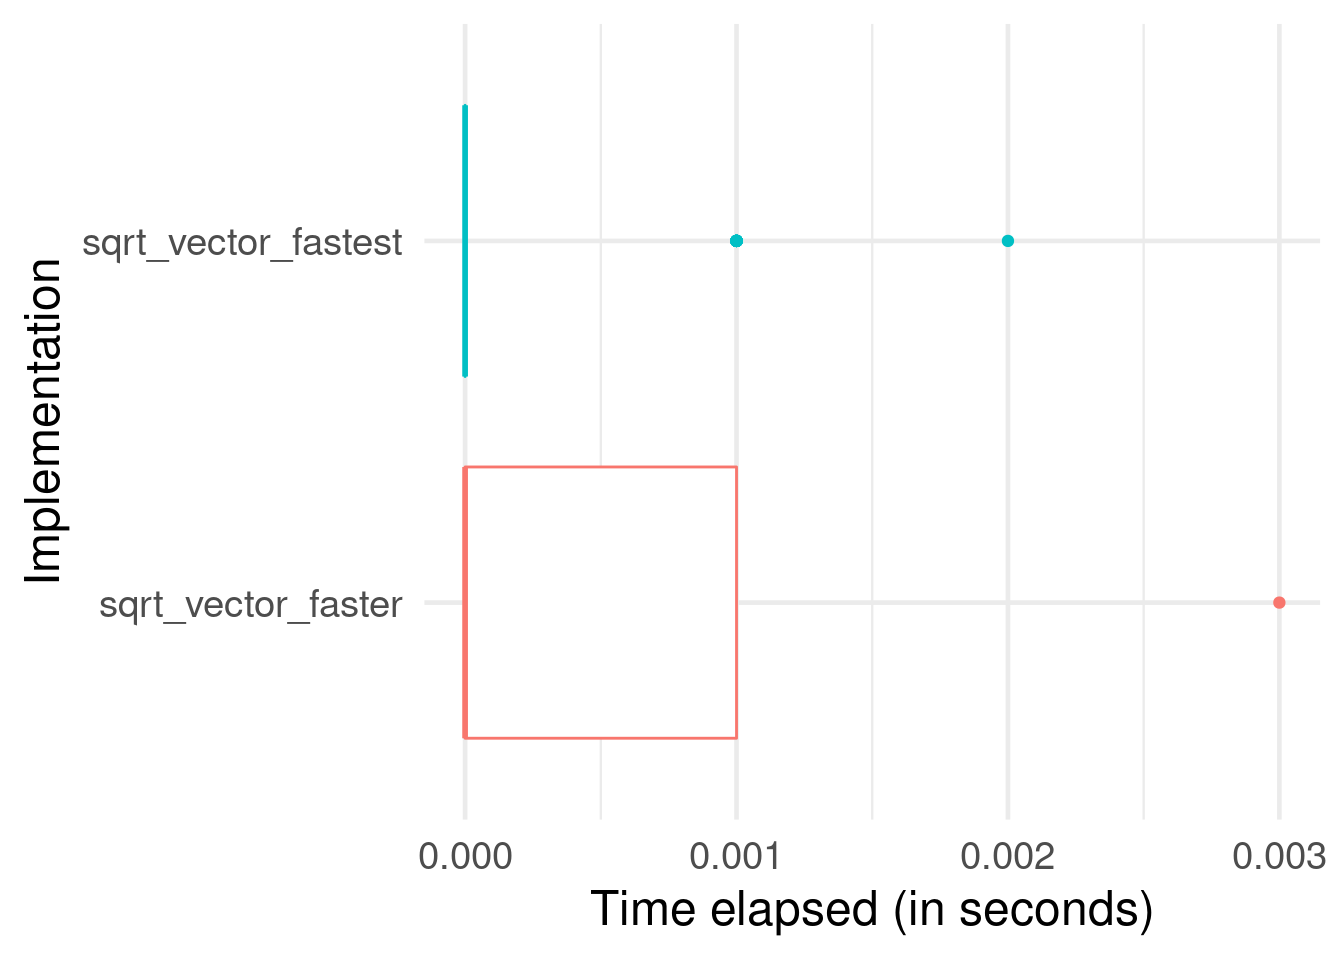
\includegraphics{bigdata_files/figure-latex/unnamed-chunk-34-1.pdf}
Clearly, the version with pre-allocation of memory (avoiding growing an object) is overall much faster. In addition, we see that the problem with the growing object in the naive implementation tends to get worse with each iteration. The take-away message for the practitioner: if possible, always initiate the ``container'' object (list, matrix, etc.) for iteration results as an empty object of the final size/dimensions.

The attentive reader and experienced R coder will have noticed by this point, that both of the functions implemented above are not really smart practice to solve the problem at hand. If you consider yourself part of this group the next subsection will make you more comfortable.

\hypertarget{vectorization-in-basic-r-functions}{%
\subsection{Vectorization in basic R functions}\label{vectorization-in-basic-r-functions}}

We can further improve the performance of this function by exploiting a particular characteristic of R: in R `everything is a vector' and many of the most basic R functions (such as math operators) are \emph{vectorized}. In simple terms, this means that an operation is implemented to directly work on vectors in such a way that it can take advantage of the similarity of each of the vector's elements. That is, R only has to figure out once how to apply a given function to a vector element in order to apply it to all elements of the vector. In a simple loop, R has to go through the same `preparatory' steps again and again in each iteration.

Following up on the problem from the previous subsection, we implement an additional function called \texttt{sqrt\_vector\_fastest} that exploits the fact that math operators in R are vectorized functions. We then re-run the same speed test as above with this function.

\begin{Shaded}
\begin{Highlighting}[]
\CommentTok{\# implementation with vectorization}
\NormalTok{sqrt\_vector\_fastest }\OtherTok{\textless{}{-}} 
     \ControlFlowTok{function}\NormalTok{(x) \{}
\NormalTok{               output }\OtherTok{\textless{}{-}}\NormalTok{  x}\SpecialCharTok{\^{}}\NormalTok{(}\DecValTok{1}\SpecialCharTok{/}\DecValTok{2}\NormalTok{)}
          \FunctionTok{return}\NormalTok{(output)}
\NormalTok{     \}}

\CommentTok{\# speed test}
\NormalTok{output\_fastest }\OtherTok{\textless{}{-}} 
     \FunctionTok{sapply}\NormalTok{(inputs, }
            \ControlFlowTok{function}\NormalTok{(x)\{ }\FunctionTok{system.time}\NormalTok{(}\FunctionTok{sqrt\_vector\_fastest}\NormalTok{(x))[}\StringTok{"elapsed"}\NormalTok{]}
\NormalTok{                 \}}
\NormalTok{            )}
\end{Highlighting}
\end{Shaded}

Let's have a look at whether this improves the function's performance further.

\begin{Shaded}
\begin{Highlighting}[]
\CommentTok{\# load packages}
\FunctionTok{library}\NormalTok{(ggplot2)}

\CommentTok{\# initiate data frame for plot}
\NormalTok{plotdata }\OtherTok{\textless{}{-}} \FunctionTok{data.frame}\NormalTok{(}\AttributeTok{time\_elapsed =} \FunctionTok{c}\NormalTok{(output\_faster, output\_fastest),}
                       \AttributeTok{input\_size =} \FunctionTok{c}\NormalTok{(input\_sizes, input\_sizes),}
                       \AttributeTok{Implementation=} \FunctionTok{c}\NormalTok{(}\FunctionTok{rep}\NormalTok{(}\StringTok{"sqrt\_vector\_faster"}\NormalTok{, }\FunctionTok{length}\NormalTok{(output\_faster)),}
                            \FunctionTok{rep}\NormalTok{(}\StringTok{"sqrt\_vector\_fastest"}\NormalTok{, }\FunctionTok{length}\NormalTok{(output\_fastest))))}

\CommentTok{\# plot}
\FunctionTok{ggplot}\NormalTok{(plotdata, }\FunctionTok{aes}\NormalTok{(}\AttributeTok{x=}\NormalTok{time\_elapsed, }\AttributeTok{y=}\NormalTok{Implementation)) }\SpecialCharTok{+}
     \FunctionTok{geom\_boxplot}\NormalTok{(}\FunctionTok{aes}\NormalTok{(}\AttributeTok{colour=}\NormalTok{Implementation),}
                          \AttributeTok{show.legend =} \ConstantTok{FALSE}\NormalTok{) }\SpecialCharTok{+}
     \FunctionTok{theme\_minimal}\NormalTok{(}\AttributeTok{base\_size =} \DecValTok{18}\NormalTok{) }\SpecialCharTok{+}
     \FunctionTok{xlab}\NormalTok{(}\StringTok{"Time elapsed (in seconds)"}\NormalTok{)}
\end{Highlighting}
\end{Shaded}

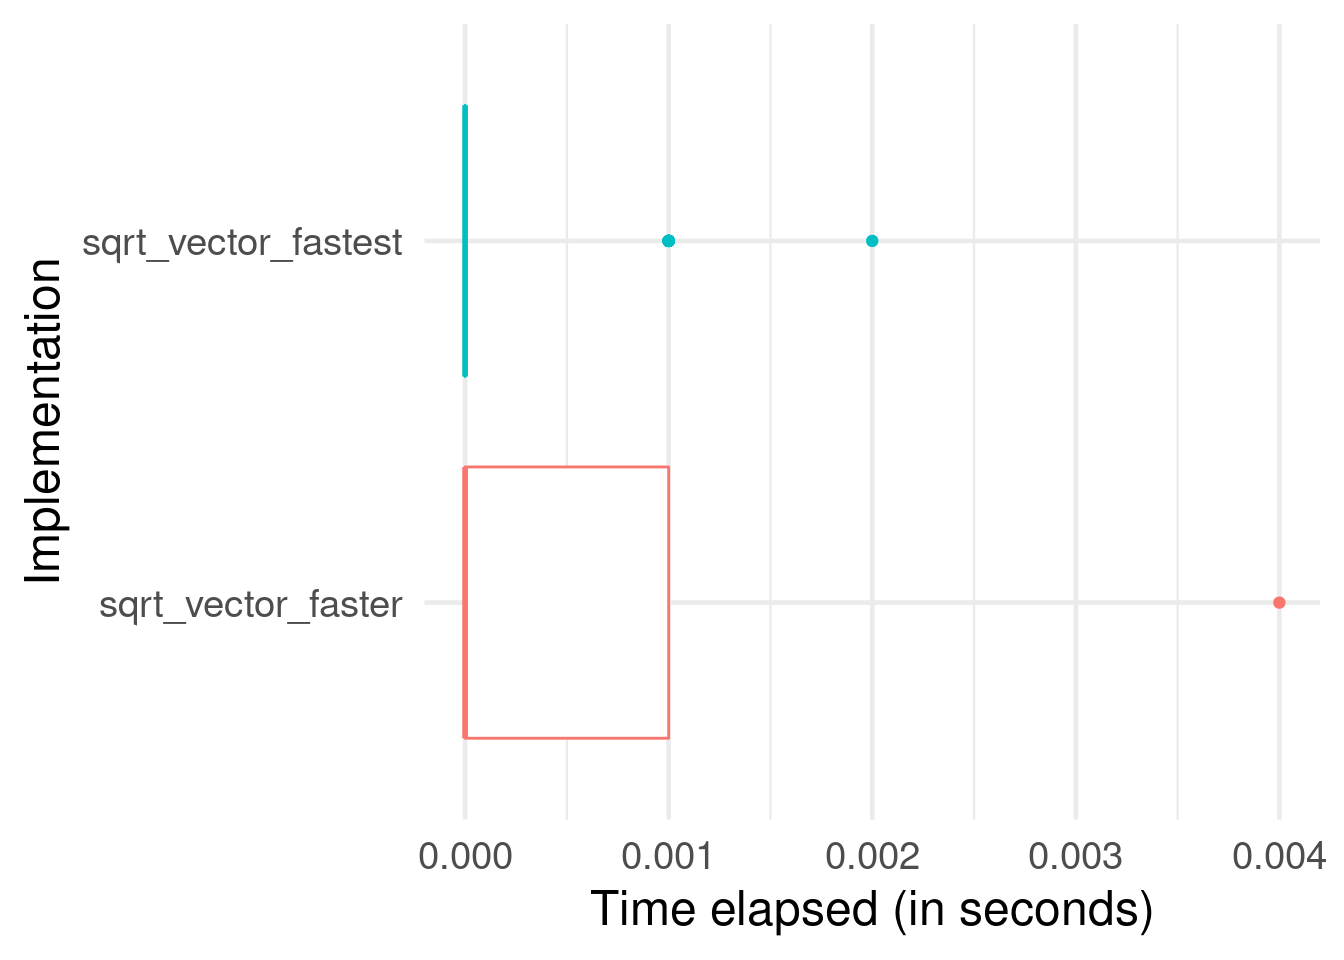
\includegraphics{bigdata_files/figure-latex/unnamed-chunk-36-1.pdf}

Clearly, the vectorized implementation is even faster. The take-away message: make use of vectorized basic R functions where possible. At this point you might wonder: why not always use vectorization over loops, when working with R? This question (and closely related similar questions) have been fiercely debated in the R online community over the last few years. Also the debate contains and has contained several (in my view) slightly misleading arguments. A simple answer to this question is: it is in fact not that simple to use \emph{actual} vectorization for every kind of problem in r. There are a number of functions often mentioned to achieve ``vectorization'' easily in R, however, they do not actually implement actual vectorization in its original technical sense (the type just demonstrated here with the R math operators). Since this point is very prominent in debates about how to improve R code, the next subsection attempts to summarize the most important aspects to keep in mind.

\hypertarget{apply-type-functions-and-vectorization}{%
\subsection{\texorpdfstring{\texttt{apply}-type functions and vectorization}{apply-type functions and vectorization}}\label{apply-type-functions-and-vectorization}}

There are basically two ways to make use of some form of ``vectorization'' instead of writing loops.

One approach is to use an \texttt{apply}-type function instead of loops. Note though, that the \texttt{apply}-type functions primarily make the writing of code more efficient. They still run a loop under the hood. Nevertheless, some \texttt{apply}-type functions might still outperform an explicit loops as they are might be better implemented.\footnote{If you know how to implement efficient for-loops in R (as you are certainly expected at this point), there is not much to gain from using an \texttt{apply}-type function instead of a loop, apart from making your code easier to read (and faster to write).}

Consider, for example, \texttt{lapply()}, a function that takes a vector (atomic or list) as input and applies a function \texttt{FUN} to each of its elements. It is a straightforward alternative to \texttt{for}-loops in many situations (and it automatically takes care of the ``growing objects'' problem discussed above). The following example shows how we can get the same result by either writing a loop or using \texttt{lapply()}. The aim of the code example is to import the \href{https://archive.ics.uci.edu/ml/datasets/Health+News+in+Twitter}{Health News in Twitter Data Set} by \citet{karami_etal2017}. The raw data consists of several text files that need to be imported to R consecutively.

The text-files are located in \texttt{data/twitter\_texts/}. For either approach of importing all of these files, we first need a list of the paths to all of the files. We can get this with \texttt{list.files()}. Also, for either approach we will make use of the \texttt{fread}-function in the \texttt{data.table}-package.

\begin{Shaded}
\begin{Highlighting}[]
\CommentTok{\# load packages}
\FunctionTok{library}\NormalTok{(data.table)}

\CommentTok{\# get a list of all file{-}paths}
\NormalTok{textfiles }\OtherTok{\textless{}{-}} \FunctionTok{list.files}\NormalTok{(}\StringTok{"data/twitter\_texts"}\NormalTok{, }\AttributeTok{full.names =} \ConstantTok{TRUE}\NormalTok{)}
\end{Highlighting}
\end{Shaded}

Now we can read in all the text files with a \texttt{for}-loop as follows.

\begin{Shaded}
\begin{Highlighting}[]
\CommentTok{\# prepare loop}
\NormalTok{all\_texts }\OtherTok{\textless{}{-}} \FunctionTok{list}\NormalTok{()}
\NormalTok{n\_files }\OtherTok{\textless{}{-}} \FunctionTok{length}\NormalTok{(textfiles)}
\FunctionTok{length}\NormalTok{(all\_texts) }\OtherTok{\textless{}{-}}\NormalTok{ n\_files}
\CommentTok{\# read all files listed in textfiles}
\ControlFlowTok{for}\NormalTok{ (i }\ControlFlowTok{in} \DecValTok{1}\SpecialCharTok{:}\NormalTok{n\_files) \{}
\NormalTok{     all\_texts[[i]] }\OtherTok{\textless{}{-}} \FunctionTok{fread}\NormalTok{(textfiles[i])}
\NormalTok{\}}
\end{Highlighting}
\end{Shaded}

The imported files are now stored as \texttt{data.table}-objects in the list \texttt{all\_texts}. With the following line of code we combine all of them in one \texttt{data.table}.

\begin{Shaded}
\begin{Highlighting}[]
\CommentTok{\# combine all in one data.table}
\NormalTok{twitter\_text }\OtherTok{\textless{}{-}} \FunctionTok{rbindlist}\NormalTok{(all\_texts)}
\CommentTok{\# check result}
\FunctionTok{str}\NormalTok{(twitter\_text)}
\end{Highlighting}
\end{Shaded}

\begin{verbatim}
## Classes 'data.table' and 'data.frame':   42422 obs. of  3 variables:
##  $ V1:integer64 585978391360221184 585947808772960257 585947807816650752 585866060991078401 585794106170839041 585733482413891584 585733481608646657 585701601131765761 ... 
##  $ V2: chr  "Thu Apr 09 01:31:50 +0000 2015" "Wed Apr 08 23:30:18 +0000 2015" "Wed Apr 08 23:30:18 +0000 2015" "Wed Apr 08 18:05:28 +0000 2015" ...
##  $ V3: chr  "Breast cancer risk test devised http://bbc.in/1CimpJF" "GP workload harming care - BMA poll http://bbc.in/1ChTBRv" "Short people's 'heart risk greater' http://bbc.in/1ChTANp" "New approach against HIV 'promising' http://bbc.in/1E6jAjt" ...
##  - attr(*, ".internal.selfref")=<externalptr>
\end{verbatim}

Alternatively, we can make use of \texttt{lapply} as follows in order to achieve exactly the same.

\begin{Shaded}
\begin{Highlighting}[]
\CommentTok{\# use lapply instead of loop}
\NormalTok{all\_texts }\OtherTok{\textless{}{-}} \FunctionTok{lapply}\NormalTok{(textfiles, fread)}
\CommentTok{\# combine all in one data.table}
\NormalTok{twitter\_text }\OtherTok{\textless{}{-}} \FunctionTok{rbindlist}\NormalTok{(all\_texts)}
\CommentTok{\# check result}
\FunctionTok{str}\NormalTok{(twitter\_text)}
\end{Highlighting}
\end{Shaded}

\begin{verbatim}
## Classes 'data.table' and 'data.frame':   42422 obs. of  3 variables:
##  $ V1:integer64 585978391360221184 585947808772960257 585947807816650752 585866060991078401 585794106170839041 585733482413891584 585733481608646657 585701601131765761 ... 
##  $ V2: chr  "Thu Apr 09 01:31:50 +0000 2015" "Wed Apr 08 23:30:18 +0000 2015" "Wed Apr 08 23:30:18 +0000 2015" "Wed Apr 08 18:05:28 +0000 2015" ...
##  $ V3: chr  "Breast cancer risk test devised http://bbc.in/1CimpJF" "GP workload harming care - BMA poll http://bbc.in/1ChTBRv" "Short people's 'heart risk greater' http://bbc.in/1ChTANp" "New approach against HIV 'promising' http://bbc.in/1E6jAjt" ...
##  - attr(*, ".internal.selfref")=<externalptr>
\end{verbatim}

Finally, we can make use of \texttt{Vectorization()} in order to ``vectorize'' our own import function (written for this example). Again, this does not make use of vectorization in its original technical sense.

\begin{Shaded}
\begin{Highlighting}[]
\CommentTok{\# initiate the import function}
\NormalTok{import\_file }\OtherTok{\textless{}{-}} 
     \ControlFlowTok{function}\NormalTok{(x) \{}
\NormalTok{          parsed\_x }\OtherTok{\textless{}{-}} \FunctionTok{fread}\NormalTok{(x)}
          \FunctionTok{return}\NormalTok{(parsed\_x)}
\NormalTok{     \}}

\CommentTok{\# \textquotesingle{}vectorize\textquotesingle{} it}
\NormalTok{import\_files }\OtherTok{\textless{}{-}} \FunctionTok{Vectorize}\NormalTok{(import\_file, }\AttributeTok{SIMPLIFY =} \ConstantTok{FALSE}\NormalTok{)}

\CommentTok{\# Apply the vectorized function}
\NormalTok{all\_texts }\OtherTok{\textless{}{-}} \FunctionTok{import\_files}\NormalTok{(textfiles)}
\NormalTok{twitter\_text }\OtherTok{\textless{}{-}} \FunctionTok{rbindlist}\NormalTok{(all\_texts)}
\CommentTok{\# check the result}
\FunctionTok{str}\NormalTok{(twitter\_text)}
\end{Highlighting}
\end{Shaded}

\begin{verbatim}
## Classes 'data.table' and 'data.frame':   42422 obs. of  3 variables:
##  $ V1:integer64 585978391360221184 585947808772960257 585947807816650752 585866060991078401 585794106170839041 585733482413891584 585733481608646657 585701601131765761 ... 
##  $ V2: chr  "Thu Apr 09 01:31:50 +0000 2015" "Wed Apr 08 23:30:18 +0000 2015" "Wed Apr 08 23:30:18 +0000 2015" "Wed Apr 08 18:05:28 +0000 2015" ...
##  $ V3: chr  "Breast cancer risk test devised http://bbc.in/1CimpJF" "GP workload harming care - BMA poll http://bbc.in/1ChTBRv" "Short people's 'heart risk greater' http://bbc.in/1ChTANp" "New approach against HIV 'promising' http://bbc.in/1E6jAjt" ...
##  - attr(*, ".internal.selfref")=<externalptr>
\end{verbatim}

The take-away message: instead of writing simple loops, use \texttt{apply}-type functions to save time writing code (and make the code easier to read) and automatically avoid memory-allocation problems.

\hypertarget{avoid-unnecessary-copying}{%
\subsection{Avoid unnecessary copying}\label{avoid-unnecessary-copying}}

The ``growing objects'' problem discussed above is only one aspect that can lead to inefficient use of memory when working with R. Another potential problem of using up more memory than necessary during an execution of an R-script, is how R handles objects/variables and their names.

Consider the following line of code.

\begin{Shaded}
\begin{Highlighting}[]
\NormalTok{a }\OtherTok{\textless{}{-}} \FunctionTok{runif}\NormalTok{(}\DecValTok{10000}\NormalTok{)}
\end{Highlighting}
\end{Shaded}

what is usually said to describe what is happening here is something along the lines of ``we initiate a variable called \texttt{a} and assign a numeric vector with 10,000 random numbers. What in fact happens is that the name \texttt{a} is assigned to the integer vector (which in turn exists at a specific memory address). Thus values do not have names but \emph{names have values}. This has important consequences for memory allocation and performance. For example, because \texttt{a} is in fact just a name attached to a value, the following does not involve any copying of values. It simply''binds'' another name, \texttt{b}, to the same value to which \texttt{a} is already bound.

\begin{Shaded}
\begin{Highlighting}[]
\NormalTok{b }\OtherTok{\textless{}{-}}\NormalTok{ a}
\end{Highlighting}
\end{Shaded}

We can prove this in two ways. First, if what I just stated was not true, the line above would actually lead to more memory being occupied by the current R session. However, this is not the case:

\begin{Shaded}
\begin{Highlighting}[]
\FunctionTok{object\_size}\NormalTok{(a)}
\end{Highlighting}
\end{Shaded}

\begin{verbatim}
## 80.05 kB
\end{verbatim}

\begin{Shaded}
\begin{Highlighting}[]
\FunctionTok{mem\_change}\NormalTok{(c }\OtherTok{\textless{}{-}}\NormalTok{ a)}
\end{Highlighting}
\end{Shaded}

\begin{verbatim}
## -635 kB
\end{verbatim}

Second, we can see that the values to which \texttt{a} and \texttt{b} are bound are stored at the same memory address. Hence, they are the same values.

\begin{Shaded}
\begin{Highlighting}[]
\CommentTok{\# load packages}
\FunctionTok{library}\NormalTok{(lobstr)}
\end{Highlighting}
\end{Shaded}

\begin{verbatim}
## 
## Attaching package: 'lobstr'
\end{verbatim}

\begin{verbatim}
## The following objects are masked from 'package:pryr':
## 
##     ast, mem_used
\end{verbatim}

\begin{Shaded}
\begin{Highlighting}[]
\CommentTok{\# check memory addresses of objects}
\FunctionTok{obj\_addr}\NormalTok{(a)}
\end{Highlighting}
\end{Shaded}

\begin{verbatim}
## [1] "0x555ade63c190"
\end{verbatim}

\begin{Shaded}
\begin{Highlighting}[]
\FunctionTok{obj\_addr}\NormalTok{(b)}
\end{Highlighting}
\end{Shaded}

\begin{verbatim}
## [1] "0x555ade63c190"
\end{verbatim}

Now you probably wonder, what happens to \texttt{b} if we modify \texttt{a}. After all, if the values to which \texttt{b} is bound are changed when we write code concerning \texttt{a}, we might end up with very surprising output. The answer is, and this is key (!), once we modify \texttt{a}, the values need to be \emph{copied} in order to ensure the integrity of \texttt{b}. Only at this point, our program will require more memory.

\begin{Shaded}
\begin{Highlighting}[]
\CommentTok{\# check the first element\textquotesingle{}s value}
\NormalTok{a[}\DecValTok{1}\NormalTok{]}
\end{Highlighting}
\end{Shaded}

\begin{verbatim}
## [1] 0.234
\end{verbatim}

\begin{Shaded}
\begin{Highlighting}[]
\NormalTok{b[}\DecValTok{1}\NormalTok{]}
\end{Highlighting}
\end{Shaded}

\begin{verbatim}
## [1] 0.234
\end{verbatim}

\begin{Shaded}
\begin{Highlighting}[]
\CommentTok{\# modify a, check memory change}
\FunctionTok{mem\_change}\NormalTok{(a[}\DecValTok{1}\NormalTok{] }\OtherTok{\textless{}{-}} \DecValTok{0}\NormalTok{)}
\end{Highlighting}
\end{Shaded}

\begin{verbatim}
## 79 kB
\end{verbatim}

\begin{Shaded}
\begin{Highlighting}[]
\CommentTok{\# check memory addresses}
\FunctionTok{obj\_addr}\NormalTok{(a)}
\end{Highlighting}
\end{Shaded}

\begin{verbatim}
## [1] "0x555b179e2e50"
\end{verbatim}

\begin{Shaded}
\begin{Highlighting}[]
\FunctionTok{obj\_addr}\NormalTok{(b)}
\end{Highlighting}
\end{Shaded}

\begin{verbatim}
## [1] "0x555ade63c190"
\end{verbatim}

Note that the entire vector needed to be copied for this. There is, of course, a lesson from all this regarding writing efficient code. Knowing how actual copying of values does occur helps avoiding unnecessary copying. The larger an object, the more time it will take to copy it in memory. Objects with a single binding get modified in place (no copying):

\begin{Shaded}
\begin{Highlighting}[]
\FunctionTok{mem\_change}\NormalTok{(d }\OtherTok{\textless{}{-}} \FunctionTok{runif}\NormalTok{(}\DecValTok{10000}\NormalTok{))}
\end{Highlighting}
\end{Shaded}

\begin{verbatim}
## 80.2 kB
\end{verbatim}

\begin{Shaded}
\begin{Highlighting}[]
\FunctionTok{mem\_change}\NormalTok{(d[}\DecValTok{1}\NormalTok{] }\OtherTok{\textless{}{-}} \DecValTok{0}\NormalTok{)}
\end{Highlighting}
\end{Shaded}

\begin{verbatim}
## 584 B
\end{verbatim}

\hypertarget{releasing-memory}{%
\subsection{Releasing memory}\label{releasing-memory}}

Closely related to the issue of copy-upon-modify, is the issue of ``releasing'' memory via ``garbage collection''. If your program uses up a lot of (too much) memory (typical for working with large data sets), all processes on your computer might substantially slow down (we will look more closely into why this is the case in the next chapter). Hence, you might want to remove/delete an object once you do not need it anymore. This can be done with the \texttt{rm()} function.

\begin{Shaded}
\begin{Highlighting}[]
\FunctionTok{mem\_change}\NormalTok{(large\_vector }\OtherTok{\textless{}{-}} \FunctionTok{runif}\NormalTok{(}\DecValTok{10}\SpecialCharTok{\^{}}\DecValTok{8}\NormalTok{))}
\end{Highlighting}
\end{Shaded}

\begin{verbatim}
## 800 MB
\end{verbatim}

\begin{Shaded}
\begin{Highlighting}[]
\FunctionTok{mem\_change}\NormalTok{(}\FunctionTok{rm}\NormalTok{(large\_vector))}
\end{Highlighting}
\end{Shaded}

\begin{verbatim}
## -800 MB
\end{verbatim}

\texttt{rm()} removes objects that are currently accessible in the global R environment. However, some objects/values might technically not be visible/accessible anymore (for example, objects that have been created in a function which has since returned the function output). To also release memory occupied by these objects you can call \texttt{gc()} (the garbage collector). While R will automatically collect the garbage once it is close to running out of memory, explicitly calling \texttt{gc} can still improve the performance of your script when working with large data sets. This is in particular the case when R is not the only data-intense process running on your computer. For example, when running an R script involving the repeated querying of data from a local SQL database and the subsequent memory-intense processing of this data in R, you can avoid using up too much memory by running \texttt{rm} and \texttt{gc} explicitly.\footnote{Note that running \texttt{gc()} takes some time, so you should not overdo it. As a rule of thumb, run \texttt{gc()} after removing a really large object.}

\hypertarget{beyond-r}{%
\subsection{Beyond R}\label{beyond-r}}

So far, we have explored idiosyncrasies of R we should be aware of when writing programs to handle and analyze large data sets. While this has shown that R has many advantages for working with data, it also revealed some aspects of R that might result in low performance compared other programming languages. A simple generic explanation for this is that R is an \href{https://en.wikipedia.org/wiki/Interpreted_language}{interpreted language}, meaning that when we execute R code, it is processed (statement by statement) by an `interpreter' that translates the code into machine code (without the user giving any specific instructions). In contrast, when writing code in a `compiled language', we first have to explicitly compile the code and then run the compiled program. Running code that is already compiled is typically much faster than running R code that has to be interpreted before it can actually be processed by the CPU.

For advanced programmers, R offers various options to directly make use of compiled programs (for example, written in C, C++, or FORTRAN). In fact several of the core R functions installed with the basic R distribution are implemented in one of these lower-level programming languages and the R function we call simply interacts with these functions.

We can actually investigate this by looking at the source code of an R function. When simply typing the name of a function (such as our \texttt{import\_file()}) to the console, R is printing the function's source code to the console.

\begin{Shaded}
\begin{Highlighting}[]
\NormalTok{import\_file}
\end{Highlighting}
\end{Shaded}

\begin{verbatim}
## function(x) {
##           parsed_x <- fread(x)
##           return(parsed_x)
##      }
## <bytecode: 0x555ad8639c18>
\end{verbatim}

However, if we do the same for function \texttt{sum}, we don't see any actual source code.

\begin{Shaded}
\begin{Highlighting}[]
\NormalTok{sum}
\end{Highlighting}
\end{Shaded}

\begin{verbatim}
## function (..., na.rm = FALSE)  .Primitive("sum")
\end{verbatim}

Instead \texttt{.Primitive()} indicates that \texttt{sum()} is actually referring to an internal function (in this case implemented in C).

While the use of functions implemented in a lower-level language is a common technique to improve the speed of `R' functions, it is particularly prominent in the context of functions/packages made to deal with large amounts of data (such as the \texttt{data.table} package).

\hypertarget{sql-basics}{%
\section{SQL basics}\label{sql-basics}}

\begin{quote}
Are tomorrow's bigger computers going to solve the problem? For some people,
yes---their data will stay the same size and computers will get big enough to
hold it comfortably. For other people it will only get worse---more powerful
computers means extraordinarily larger datasets. If you are likely to be in this
latter group, you might want to get used to working with databases now.
\end{quote}

\citep{burns_2011}

The Structured Query Language (SQL) has become a bread-and-butter tool for data analysts and data scientists due to its broad application in systems used to store large amounts of data. While traditionally only encountered in the context of structured data stored in relational database management systems, some versions of it are now also used to query data from data warehouse systems (e.g.~Amazon Redshift) and even to query massive amounts (terabytes or even petabytes) of data stored in data lakes (e.g., Amazon Athena). In all of these applications, SQL's purpose (from the data analytics' perspective) is to provide a convenient and efficient way to query data from mass storage for analysis. Instead of importing a CSV file into R and then filtering it in order to get to the analytic data set, we use SQL to express how the analytic data set should look like (which variables and rows should be included).

The latter point is very important to keep in mind when already having experience with a language like R and learning SQL for the first time. In R we write code to instruct the computer what to do with the data. For example, we tell it to import a csv file called \texttt{economics.csv} as a \texttt{data.table}, then we instruct it to remove observations which are older than a certain date according to the \texttt{date} column, then we instruct it to compute the average of the \texttt{unemploy} column values for each year based on the \texttt{date} column and then return the result as a separate data frame.

\begin{Shaded}
\begin{Highlighting}[]
\CommentTok{\# import data}
\NormalTok{econ }\OtherTok{\textless{}{-}} \FunctionTok{read.csv}\NormalTok{(}\StringTok{"data/economics.csv"}\NormalTok{)}

\CommentTok{\# filter}
\NormalTok{econ2 }\OtherTok{\textless{}{-}}\NormalTok{ econ[}\StringTok{"1968{-}01{-}01"}\SpecialCharTok{\textless{}=}\NormalTok{econ}\SpecialCharTok{$}\NormalTok{date,]}

\CommentTok{\# compute yearly averages (basic R approach)}
\NormalTok{econ2}\SpecialCharTok{$}\NormalTok{year }\OtherTok{\textless{}{-}}\NormalTok{ lubridate}\SpecialCharTok{::}\FunctionTok{year}\NormalTok{(econ2}\SpecialCharTok{$}\NormalTok{date)}
\NormalTok{years }\OtherTok{\textless{}{-}} \FunctionTok{unique}\NormalTok{(econ2}\SpecialCharTok{$}\NormalTok{year)}
\NormalTok{averages }\OtherTok{\textless{}{-}} \FunctionTok{sapply}\NormalTok{(years, }\AttributeTok{FUN =} \ControlFlowTok{function}\NormalTok{(x) }\FunctionTok{mean}\NormalTok{(econ2[econ2}\SpecialCharTok{$}\NormalTok{year}\SpecialCharTok{==}\NormalTok{x,}\StringTok{"unemploy"}\NormalTok{]))}
\NormalTok{output }\OtherTok{\textless{}{-}} \FunctionTok{data.frame}\NormalTok{(}\AttributeTok{year=}\NormalTok{years, }\AttributeTok{average\_unemploy=}\NormalTok{averages)}

\CommentTok{\# inspect the first few lines of the result}
\FunctionTok{head}\NormalTok{(output)}
\end{Highlighting}
\end{Shaded}

\begin{verbatim}
##   year average_unemploy
## 1 1968             2797
## 2 1969             2830
## 3 1970             4127
## 4 1971             5022
## 5 1972             4876
## 6 1973             4359
\end{verbatim}

In contrast, when using SQL we write code that describes how the final result is supposed to look like. The SQL engine processing the code then takes care of the rest and returns the result in the most efficient way.\footnote{In particular, the user does not need to explicitly instruct SQL at which point in the process which part (filtering, selecting variables, aggregating, creating new variables etc.) of the query should be processed. SQL will automatically find the most efficient way to process the query.}

\begin{Shaded}
\begin{Highlighting}[]
\KeywordTok{SELECT} 
\NormalTok{strftime(}\StringTok{\textquotesingle{}\%Y\textquotesingle{}}\NormalTok{, \textasciigrave{}date\textasciigrave{})  }\KeywordTok{AS} \DataTypeTok{year}\NormalTok{,}
\FunctionTok{AVG}\NormalTok{(unemploy) }\KeywordTok{AS}\NormalTok{ average\_unemploy}
\KeywordTok{FROM}\NormalTok{ econ}
\KeywordTok{WHERE} \OtherTok{"1968{-}01{-}01"}\OperatorTok{\textless{}=}\NormalTok{\textasciigrave{}date\textasciigrave{}}
\KeywordTok{GROUP} \KeywordTok{BY} \DataTypeTok{year} \KeywordTok{LIMIT} \DecValTok{6}\NormalTok{;}
\end{Highlighting}
\end{Shaded}

\begin{table}

\caption{\label{tab:unnamed-chunk-54}6 records}
\centering
\begin{tabular}[t]{l|r}
\hline
year & average\_unemploy\\
\hline
1968 & 2797\\
\hline
1969 & 2830\\
\hline
1970 & 4127\\
\hline
1971 & 5022\\
\hline
1972 & 4876\\
\hline
1973 & 4359\\
\hline
\end{tabular}
\end{table}

For the moment, we will only focus on the code and ignore the underlying hardware and database concepts (those will be discussed in more detail in chapter 5).

\hypertarget{first-steps-in-sqlite}{%
\subsection{First steps in SQL(ite)}\label{first-steps-in-sqlite}}

In order to get familiar with coding in SQL, we work with a free and easy-to-use version of SQL called \emph{SQLite}. \href{https://sqlite.org/index.html}{SQLite} is a free full-featured SQL database engine widely used across platforms. It comes usually pre-installed with Windows and Mac/OSX distributions and has (from the user's perspective) all the core features of more sophisticated SQL versions. Unlike the more sophisticated SQL systems, SQLite does not rely explicitly on a client/server-model. That is, there is no need to set up your database on a server and then query it from a client interface. In fact, setting it up is straightforward. In the terminal, we can directly call SQLite as a command-line tool (on most modern computers the command is now \texttt{sqlite3}, SQLite version 3).

In this first code example, we set up an SQLite database using the command line. In the file structure of the book repository, we first switch to the data directory.

\begin{Shaded}
\begin{Highlighting}[]
\BuiltInTok{cd}\NormalTok{ data }
\end{Highlighting}
\end{Shaded}

With one simple command, we start up SQLite, create a new database called \texttt{mydb.sqlite} and connect to the newly created database.\footnote{If there is already a database called \texttt{mydb.sqlite} in this folder, the same command would simply start up SQLite and connect to the existing database.}

\begin{Shaded}
\begin{Highlighting}[]
\ExtensionTok{sqlite3}\NormalTok{ mydb.sqlite}
\end{Highlighting}
\end{Shaded}

This created a new file \texttt{mydb.sqlite} in our \texttt{data} directory which contains the newly created database. And, we are now running \texttt{sqlite} in the terminal (indicated with the \texttt{sqlite\textgreater{}}. This means we can now type SQL code in the terminal to run queries and other SQL commands.

At this point, the newly created database does not contain any data yet. There are no tables in it. We can see this by running the \texttt{.tables} command.

\begin{Shaded}
\begin{Highlighting}[]
\NormalTok{.}\KeywordTok{tables}
\end{Highlighting}
\end{Shaded}

As expected, nothing is returned. Now, let's create our first table and import the \texttt{economics.csv} data set to it. In SQLite, it makes sense to first set up an empty table in which all column data types are defined before importing data from a CSV-file to it. If a CSV is directly imported to a new table (without type definitions), all columns will be set to \texttt{TEXT} (similar to \texttt{character} in R) by default. Setting the right data type for each variable follows essentially the same logic as setting the data types of a data frame's columns in R (with the difference that in SQL this also affects how the data is stored on disk).\footnote{The most commonly used data types in SQL all have a very similar R equivalent: \texttt{DATE} is like \texttt{Date} in R, \texttt{REAL} like \texttt{numeric/double}, \texttt{INTEGER} like \texttt{integer}, and \texttt{TEXT} like \texttt{character}.}

In a first step, we thus create a new table called \texttt{econ}.

\begin{Shaded}
\begin{Highlighting}[]
\CommentTok{{-}{-} Create the new table}
\KeywordTok{CREATE} \KeywordTok{TABLE}\NormalTok{ econ(}
\OtherTok{"date"} \DataTypeTok{DATE}\NormalTok{,}
\OtherTok{"pce"} \DataTypeTok{REAL}\NormalTok{,}
\OtherTok{"pop"} \DataTypeTok{REAL}\NormalTok{,}
\OtherTok{"psavert"} \DataTypeTok{REAL}\NormalTok{,}
\OtherTok{"uempmed"} \DataTypeTok{REAL}\NormalTok{,}
\OtherTok{"unemploy"} \DataTypeTok{INTEGER}
\NormalTok{);}
\end{Highlighting}
\end{Shaded}

Then, we can import the data from the csv file, by first switching to CSV mode via the command \texttt{.mode\ csv} and then importing the data to \texttt{econ} with \texttt{.import}. The \texttt{.import} command expects as a first argument the path to the CSV file on disk and as a second argument the name of the table to import the data to.

\begin{Shaded}
\begin{Highlighting}[]
\CommentTok{{-}{-} prepare import}
\NormalTok{.}\KeywordTok{mode}\NormalTok{ csv}
\CommentTok{{-}{-} import data from csv}
\NormalTok{.import }\CommentTok{{-}{-}skip 1 economics.csv econ}
\end{Highlighting}
\end{Shaded}

Now we can have a look at the new database table in SQLite. \texttt{.tables} shows that we now have one table called \texttt{econ} in our database and \texttt{.schema} displays the structure of the new \texttt{econ} table.

\begin{verbatim}
.tables
\end{verbatim}

\begin{verbatim}
# econ
\end{verbatim}

\begin{verbatim}
.schema econ
\end{verbatim}

\begin{verbatim}
# CREATE TABLE econ(
# "date" DATE,
# "pce" REAL,
# "pop" REAL,
# "psavert" REAL,
# "uempmed" REAL,
# "unemploy" INTEGER
# );
\end{verbatim}

With this, we can start querying data with SQLite. In order to make the query results easier to read, we first set two options regarding how query results are displayed in the terminal. \texttt{.header\ on} enables the display of the column names in the returned query results. And \texttt{.mode\ columns} arranges the query results in columns.

\begin{Shaded}
\begin{Highlighting}[]
\NormalTok{.}\KeywordTok{header} \KeywordTok{on}
\end{Highlighting}
\end{Shaded}

\begin{Shaded}
\begin{Highlighting}[]
\NormalTok{.}\KeywordTok{mode} \KeywordTok{columns}
\end{Highlighting}
\end{Shaded}

In our first query, we select all (\texttt{*}) variable values of the observation of January 1968.

\begin{Shaded}
\begin{Highlighting}[]
\KeywordTok{select} \OperatorTok{*} \KeywordTok{from}\NormalTok{ econ }\KeywordTok{where} \DataTypeTok{date} \OperatorTok{=} \StringTok{\textquotesingle{}1968{-}01{-}01\textquotesingle{}}\NormalTok{;}
\end{Highlighting}
\end{Shaded}

\begin{table}

\caption{\label{tab:unnamed-chunk-62}1 records}
\centering
\begin{tabular}[t]{l|r|r|r|r|r}
\hline
date & pce & pop & psavert & uempmed & unemploy\\
\hline
1968-01-01 & 531.5 & 199808 & 11.7 & 5.1 & 2878\\
\hline
\end{tabular}
\end{table}

\hypertarget{simple-queries}{%
\subsubsection{Simple queries}\label{simple-queries}}

Now let's select all dates and unemployment values of observations with more than 15 million unemployed, ordered by date.

\begin{Shaded}
\begin{Highlighting}[]
\KeywordTok{select} \DataTypeTok{date}\NormalTok{, }
\NormalTok{unemploy }\KeywordTok{from}\NormalTok{ econ }
\KeywordTok{where}\NormalTok{ unemploy }\OperatorTok{\textgreater{}} \DecValTok{15000}
\KeywordTok{order} \KeywordTok{by} \DataTypeTok{date}\NormalTok{;}
\end{Highlighting}
\end{Shaded}

\begin{table}

\caption{\label{tab:unnamed-chunk-63}9 records}
\centering
\begin{tabular}[t]{l|r}
\hline
date & unemploy\\
\hline
2009-09-01 & 15009\\
\hline
2009-10-01 & 15352\\
\hline
2009-11-01 & 15219\\
\hline
2009-12-01 & 15098\\
\hline
2010-01-01 & 15046\\
\hline
2010-02-01 & 15113\\
\hline
2010-03-01 & 15202\\
\hline
2010-04-01 & 15325\\
\hline
2010-11-01 & 15081\\
\hline
\end{tabular}
\end{table}

\hypertarget{joins}{%
\subsection{Joins}\label{joins}}

So far, we have only considered queries involving one table of data. However, SQL provides a very efficient way to join data from various tables. Again, the way of writing SQL code is the same: you describe how the final table should look like and from where the data is to be selected.

Let's extend the previous example by importing an additional table to our \texttt{mydb.sqlite}. The additional data is stored in the file \texttt{inflation.csv} in the book's data folder and contains information on the US yearly inflation rate measured in percent.\footnote{Like the data stored in \texttt{economics.csv}, the data stored in \texttt{inflation.csv} is provided by the Federal Reserve Bank's (FRED){[}\url{https://fred.stlouisfed.org/}{]} website.}

\begin{Shaded}
\begin{Highlighting}[]
\CommentTok{{-}{-} Create the new table}
\KeywordTok{CREATE} \KeywordTok{TABLE}\NormalTok{ inflation(}
\OtherTok{"date"} \DataTypeTok{DATE}\NormalTok{,}
\OtherTok{"inflation\_percent"} \DataTypeTok{REAL}
\NormalTok{);}

\CommentTok{{-}{-} prepare import}
\NormalTok{.}\KeywordTok{mode}\NormalTok{ csv}
\CommentTok{{-}{-} import data from csv}
\NormalTok{.import }\CommentTok{{-}{-}skip 1 inflation.csv inflation}
\CommentTok{{-}{-} switch back to column mode }
\NormalTok{.}\KeywordTok{mode} \KeywordTok{columns}
\end{Highlighting}
\end{Shaded}

Note that the data stored in \texttt{econ} contains monthly observations, while \texttt{inflation} contains yearly observations. We can thus only meaningfully combine the two data sets at the level of years. Again using the combination of data sets in R as a reference point, here is what we would like to achieve expressed in R. The aim is to get a table that serves as basis for a \href{https://en.wikipedia.org/wiki/Phillips_curve}{Phillips curve} plot, with yearly observations and the variables \texttt{year}, \texttt{average\_unemp\_percent}, and \texttt{inflation\_percent}.

\begin{Shaded}
\begin{Highlighting}[]
\CommentTok{\# import data}
\NormalTok{econ }\OtherTok{\textless{}{-}} \FunctionTok{read.csv}\NormalTok{(}\StringTok{"data/economics.csv"}\NormalTok{)}
\NormalTok{inflation }\OtherTok{\textless{}{-}} \FunctionTok{read.csv}\NormalTok{(}\StringTok{"data/inflation.csv"}\NormalTok{)}

\CommentTok{\# prepare variable to match observations}
\NormalTok{econ}\SpecialCharTok{$}\NormalTok{year }\OtherTok{\textless{}{-}}\NormalTok{ lubridate}\SpecialCharTok{::}\FunctionTok{year}\NormalTok{(econ}\SpecialCharTok{$}\NormalTok{date)}
\NormalTok{inflation}\SpecialCharTok{$}\NormalTok{year }\OtherTok{\textless{}{-}}\NormalTok{ lubridate}\SpecialCharTok{::}\FunctionTok{year}\NormalTok{(inflation}\SpecialCharTok{$}\NormalTok{date)}

\CommentTok{\# create final output}
\NormalTok{years }\OtherTok{\textless{}{-}} \FunctionTok{unique}\NormalTok{(econ}\SpecialCharTok{$}\NormalTok{year)}
\NormalTok{averages }\OtherTok{\textless{}{-}} \FunctionTok{sapply}\NormalTok{(years, }\AttributeTok{FUN =} \ControlFlowTok{function}\NormalTok{(x) \{}
        \FunctionTok{mean}\NormalTok{(econ[econ}\SpecialCharTok{$}\NormalTok{year}\SpecialCharTok{==}\NormalTok{x,}\StringTok{"unemploy"}\NormalTok{]}\SpecialCharTok{/}\NormalTok{econ[econ}\SpecialCharTok{$}\NormalTok{year}\SpecialCharTok{==}\NormalTok{x,}\StringTok{"pop"}\NormalTok{])}\SpecialCharTok{*}\DecValTok{100}
        
\NormalTok{\} )}
\NormalTok{unemp }\OtherTok{\textless{}{-}} \FunctionTok{data.frame}\NormalTok{(}\AttributeTok{year=}\NormalTok{years,}
                     \AttributeTok{average\_unemp\_percent=}\NormalTok{averages)}

\CommentTok{\# combine via the year column}
\CommentTok{\# keep all rows of econ}
\NormalTok{output}\OtherTok{\textless{}{-}} \FunctionTok{merge}\NormalTok{(unemp, inflation[, }\FunctionTok{c}\NormalTok{(}\StringTok{"year"}\NormalTok{, }\StringTok{"inflation\_percent"}\NormalTok{)], }\AttributeTok{by=}\StringTok{"year"}\NormalTok{)}


\CommentTok{\# inspect output}
\FunctionTok{head}\NormalTok{(output)}
\end{Highlighting}
\end{Shaded}

\begin{verbatim}
##   year average_unemp_percent inflation_percent
## 1 1967                 1.512             2.773
## 2 1968                 1.394             4.272
## 3 1969                 1.396             5.462
## 4 1970                 2.013             5.838
## 5 1971                 2.419             4.293
## 6 1972                 2.324             3.272
\end{verbatim}

Now let's look at how the same table can be created in SQLite.

\begin{Shaded}
\begin{Highlighting}[]
\KeywordTok{SELECT} 
\NormalTok{strftime(}\StringTok{\textquotesingle{}\%Y\textquotesingle{}}\NormalTok{, econ.}\DataTypeTok{date}\NormalTok{)  }\KeywordTok{AS} \DataTypeTok{year}\NormalTok{,}
\FunctionTok{AVG}\NormalTok{(unemploy}\OperatorTok{/}\NormalTok{pop)}\OperatorTok{*}\DecValTok{100} \KeywordTok{AS}\NormalTok{ average\_unemp\_percent,}
\NormalTok{inflation\_percent}
\KeywordTok{FROM}\NormalTok{ econ }\KeywordTok{INNER} \KeywordTok{JOIN}\NormalTok{ inflation }\KeywordTok{ON} \DataTypeTok{year} \OperatorTok{=}\NormalTok{ strftime(}\StringTok{\textquotesingle{}\%Y\textquotesingle{}}\NormalTok{, inflation.}\DataTypeTok{date}\NormalTok{)}
\KeywordTok{GROUP} \KeywordTok{BY} \DataTypeTok{year}
\end{Highlighting}
\end{Shaded}

\begin{table}

\caption{\label{tab:unnamed-chunk-67}Displaying records 1 - 6}
\centering
\begin{tabular}[t]{l|r|r}
\hline
year & average\_unemp\_percent & inflation\_percent\\
\hline
1967 & 1.512 & 2.773\\
\hline
1968 & 1.394 & 4.272\\
\hline
1969 & 1.397 & 5.462\\
\hline
1970 & 2.013 & 5.838\\
\hline
1971 & 2.419 & 4.293\\
\hline
1972 & 2.324 & 3.272\\
\hline
\end{tabular}
\end{table}

When done working with the database, we can exit SQLite with the \texttt{.quit} command.

\hypertarget{hardware-computing-resources}{%
\chapter{Hardware: Computing Resources}\label{hardware-computing-resources}}

In order to better understand how we can use the available computing resources most efficiently in an analytics task, this chapter first briefly reviews the most basic hardware components and how they matter for computation. We then look at each of these components (and additional specialized components) through the lens of Big Data. That is, for each component, we look at how this component becomes a crucial bottleneck when processing large amounts of data and what we can do about it in R.

\hypertarget{components-of-a-standard-computing-environment}{%
\section{Components of a standard computing environment}\label{components-of-a-standard-computing-environment}}

Figure \ref{components} illustrates the key components of a standard computing environment to process digital data. In our case, these components serve the purpose of computing a statistic, given a large dataset as input.

\begin{figure}

{\centering 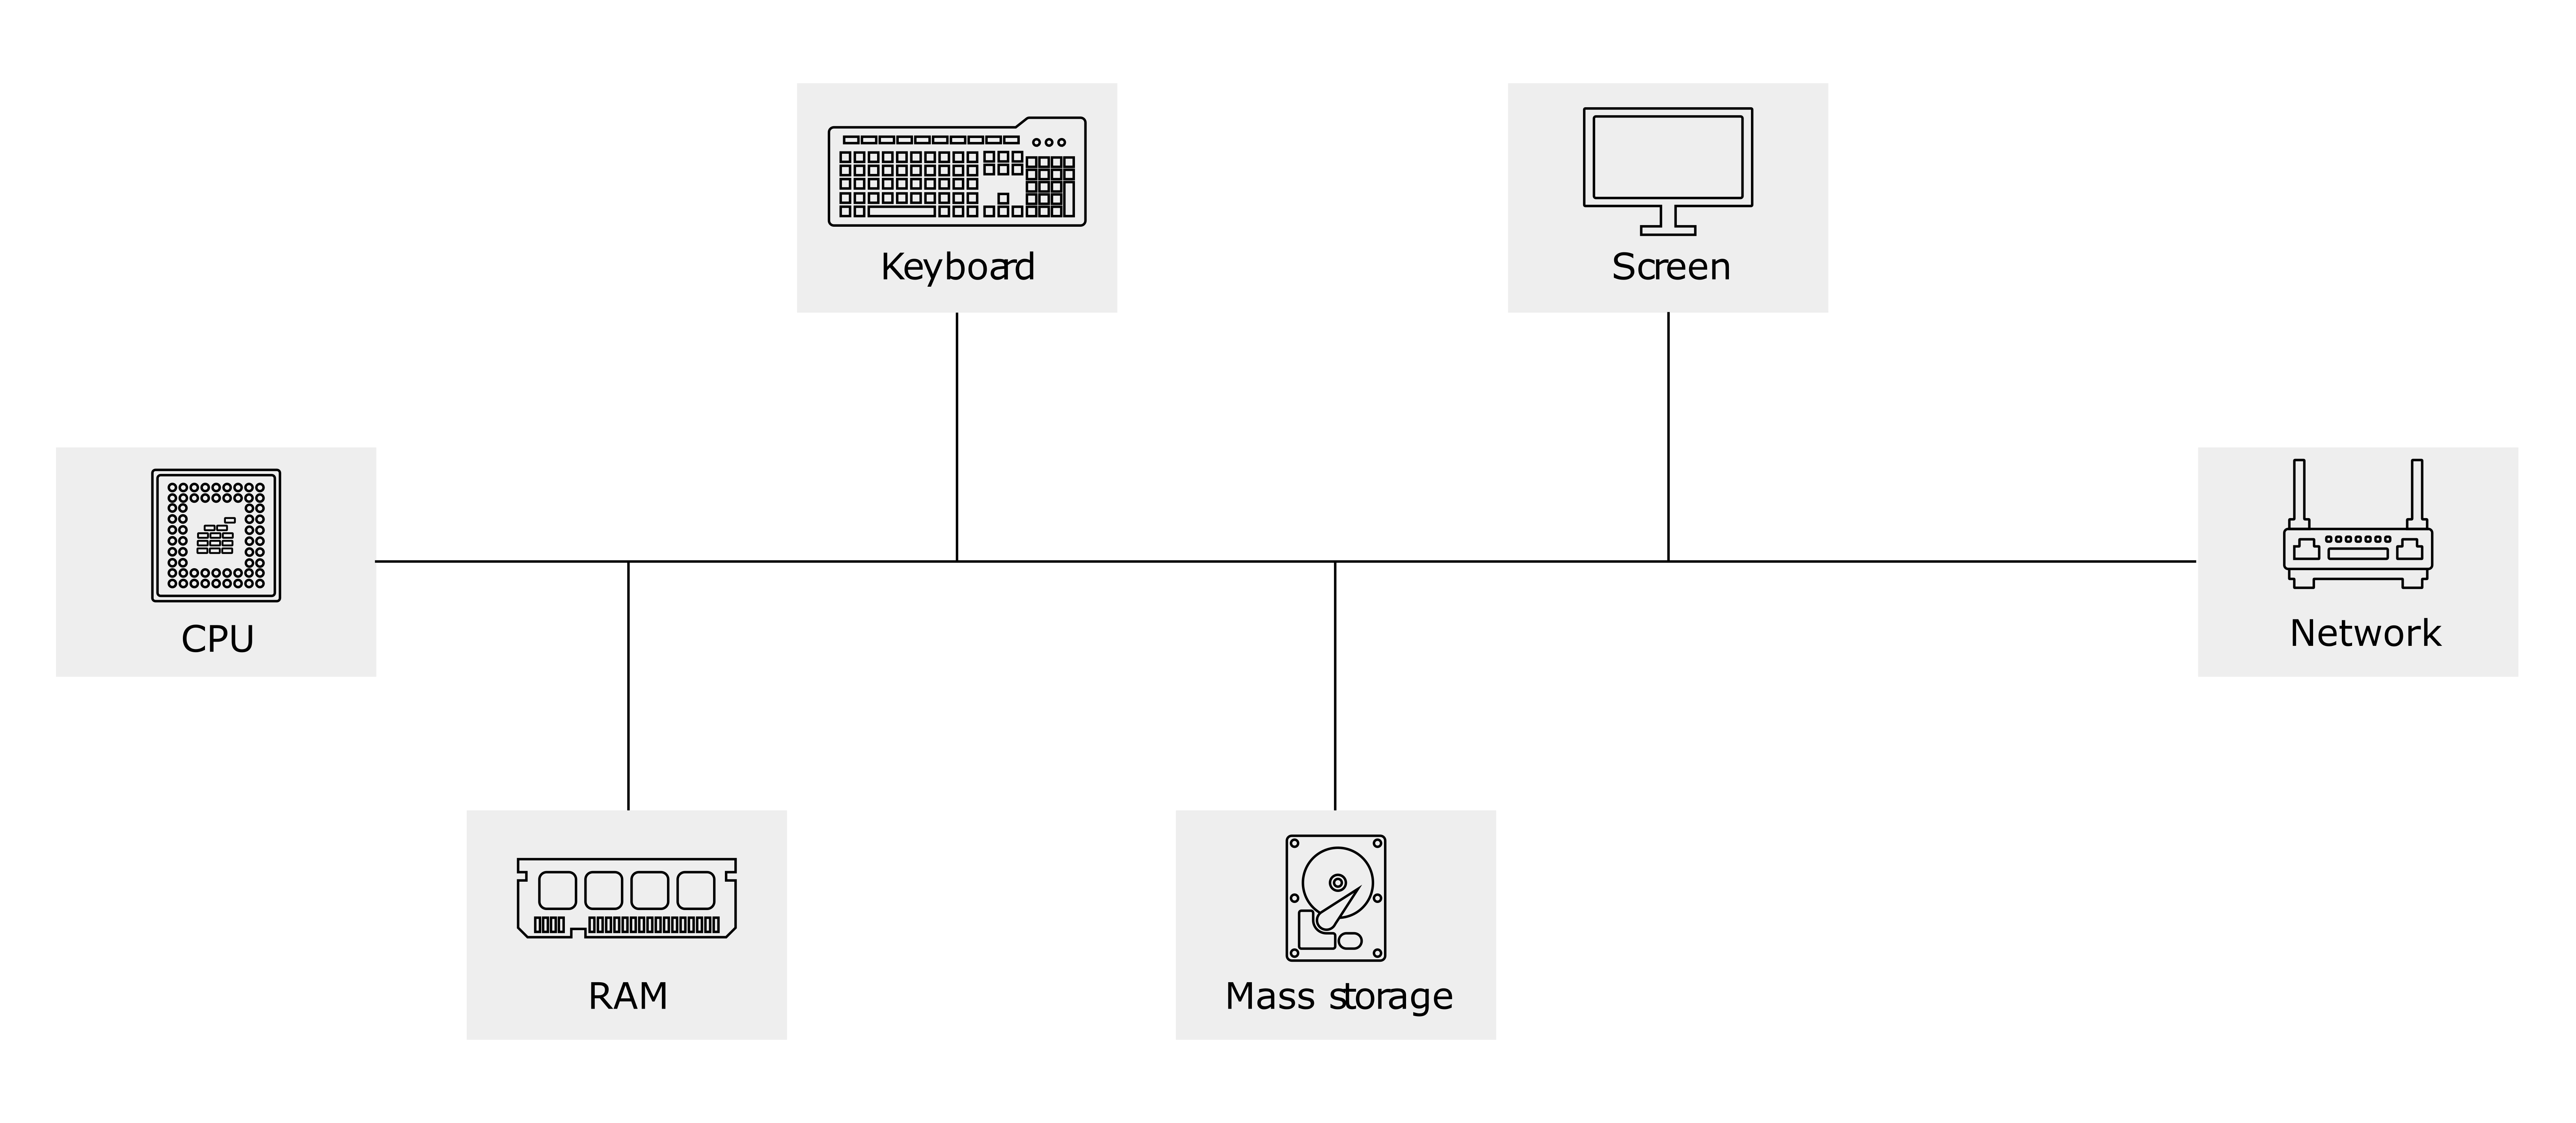
\includegraphics[width=0.99\linewidth]{img/computing_environment} 

}

\caption{Basic components of a standard computing environment.}\label{fig:components}
\end{figure}



\begin{itemize}
\item
  \emph{Mass storage} refers to the type of computer memory we use to store data in the long run. This is what we call the \emph{hard drive} or \emph{hard disk}.
\item
  In order to work with data (e.g., in R), it first has to be loaded into the \emph{memory} of our computer. More specifically, into the random access memory (\emph{RAM}). Typically, data is only loaded in the RAM for as long as we are working with it.
\item
  The component actually \emph{processing} data is the central processing unit (CPU). When using R to process data, R commands are translated into complex combinations of a small sets of basic operations, which the \emph{CPU} then executes.
\end{itemize}

For this and the later chapters, consider the main difference between common `data analytics' and `Big Data analytics' to be the following: in a Big Data analytics context, the standard usage of one or several of the standard hardware components in your local computer fails to work or works very inefficiently because the amount of data overwhelms its normal capacity.

From the hardware perspective, there are two basic strategies to cope with the situation that one of these components is overwhelmed by the amount of data:

\begin{itemize}
\tightlist
\item
  \emph{Scale up (`horizontal scaling')}: Extend the physical capacity of the affected component by building a system with a large amount of RAM shared between applications. This sounds like a trivial solution (`if RAM is too small, buy more RAM\ldots{}'), but in practice it can be very expensive.
\item
  \emph{Scale out (`vertical scaling')}: Distribute the workload over several computers (or separate components of a system).
\end{itemize}

From a software perspective, there are many (context-specific) strategies that can help us to use the resources available more efficiently in order to process large amounts of data. In the following sub-sections, we first get an idea of what we mean by capacity and \emph{big} regarding the most important hardware components. First we focus on mass storage and memory, then on the CPU, and finally on new alternatives to the CPU.

\hypertarget{mass-storage}{%
\section{Mass storage}\label{mass-storage}}

In a simple computing environment, the mass storage device (hard disk) is where the data is stored to be analyzed. So, in what units do we measure the size of datasets and consequently the mass storage capacity of a computer? The smallest unit of information in computing/digital data is called a \emph{bit} (from \emph{bi}nary dig\emph{it}; abbrev. `b') and can take one of two (symbolic) values, either a \texttt{0} or a \texttt{1} (``off'' or ``on''). Consider, for example, the decimal number \texttt{139}. Written in the binary system, \texttt{139} corresponds to the binary number \texttt{10001011}. In order to store this number on a hard disk, we require a capacity of 8 bits, or one \emph{byte} (1 byte = 8 bits; abbrev. `B'). Historically, one byte encoded a single character of text (i.e., in the ASCII character encoding system). When thinking of a given dataset in its raw/binary representation, we can simply think of it as a row of \texttt{0}s and \texttt{1}s.

Bigger units for storage capacity usually build on bytes, for example:

\begin{itemize}
\tightlist
\item
  \(1 \text{ kilobyte (KB)} = 1000^{1} \approx 2^{10} \text{ bytes}\)
\item
  \(1 \text{ megabyte (MB)} = 1000^{2} \approx 2^{20} \text{ bytes}\)
\item
  \(1 \text{ gigabyte (GB)} = 1000^{3} \approx 2^{30} \text{ bytes}\)
\end{itemize}

Currently, a common laptop or desktop computer has several hundred GBs of mass storage capacity. The problems related to a lack of mass storage capacity in Big Data analytics are likely the easiest to understand. Suppose you collect large amounts of data from an online source such as the Twitter API (application programming interface). At some point, R will throw an error and stop the data collection procedure as the operating system will not allow R to use up more disk space. The simplest solution to this problem is to clean up your hard disk: empty the trash, archive files in the cloud or on an external drive and delete them on the main disk, etc. In addition, there are some easy-to-learn tricks to use from within R to save some disk space.

\hypertarget{avoid-redundancies}{%
\subsection{Avoid redundancies}\label{avoid-redundancies}}

Different formats for structuring data stored on disk use up more or less space. A simple example is the comparison of JSON (JavaScript Object Notation) and CSV (Comma Separated Values) -- both data structures that are widely used to store data for analytics purposes. JSON is much more flexible in that it allows the definition of arbitrarily complex hierarchical data structures (and even allows for hints at data types). However, this flexibility comes with some overhead in the usage of special characters to define the structure. Consider the following JSON excerpt of an economic time series fetched from the Federal Reserve's \href{https://fred.stlouisfed.org/docs/api/fred/series_observations.html\#example_json}{FRED API}.

\begin{verbatim}
{
    "realtime_start": "2013-08-14",
    "realtime_end": "2013-08-14",
    "observation_start": "1776-07-04",
    "observation_end": "9999-12-31",
    "units": "lin",
    "output_type": 1,
    "file_type": "json",
    "order_by": "observation_date",
    "sort_order": "asc",
    "count": 84,
    "offset": 0,
    "limit": 100000,
    "observations": [
        {
            "realtime_start": "2013-08-14",
            "realtime_end": "2013-08-14",
            "date": "1929-01-01",
            "value": "1065.9"
        },
        {
            "realtime_start": "2013-08-14",
            "realtime_end": "2013-08-14",
            "date": "1930-01-01",
            "value": "975.5"
        },
        ...,
        {
            "realtime_start": "2013-08-14",
            "realtime_end": "2013-08-14",
            "date": "2012-01-01",
            "value": "15693.1"
        }
    ]
}
\end{verbatim}

The JSON format is very practical here in separating metadata (such as what time frame is covered by this dataset, etc.) in the first few lines on top from the actual data in \texttt{"observations"} further down. However, note that due to this structure, the key names like \texttt{"date"}, and \texttt{"value"} occur for each observation in that time series. In addition, \texttt{"realtime\_start"} and \texttt{"realtime\_end"} occur both in the metadata section and again in each observation. Each of those occurrences costs some bytes of storage space on your hard disk but does not add any information once you have parsed and imported the time series into R. The same information could also be stored in a more efficient way on your hard disk by simply storing the metadata in a separate text file and the actual observations in a CSV file (in a table-like structure):

\begin{verbatim}
"date","value"
"1929-01-01", "1065.9"
"1930-01-01", "975.5"

...,

"2012-01-01", 15693.1"
\end{verbatim}

In fact, in that particular example, storing the data in JSON format would take up more than double the hard-disk space as CSV. Of course, this is not to say that one should generally store data in CSV files. In many situations, you might really have to rely on JSON's flexibility to represent more complex structures. However, in practice it is very much worthwhile to think about whether you can improve storage efficiency by simply storing raw data in a different format.

Another related point to storing data in CSV files is to remove redundancies by splitting the data into several tables/CSV files, whereby each table contains the variables exclusively describing the type of observation in it. For example, when analyzing customer data for marketing purposes, the dataset stored in one CSV file might be at the level of individual purchases. That is, each row contains both information on what has been purchased on which day by which customer as well as additional variables describing the customer (such as customer id, name, address, etc.). Instead of keeping all of this data in one file, we could split it into two files, where one only contains the order ids and corresponding customer ids as well as attributes of individual orders (but not additional attributes of the customers themselves) and the other contains the customer ids and all customer attributes. Thereby, we avoid redundancies in the form of repeatedly storing the same values of customer attributes (like name and address) for each order.\footnote{This concept of organizing data into several tables is the basis of relational database management systems, which we will look at in more detail in Chapter 5. However, the basic idea is also very useful for storing raw data efficiently even if there is no intention to later build a database and run SQL queries on it.}

\hypertarget{data-compression}{%
\subsection{Data compression}\label{data-compression}}

Data compression essentially follows from the same basic idea of avoiding redundancies in data storage as the simple approaches discussed above. However, it happens on a much more fundamental level. Data compression algorithms encode the information contained in the original representation of the data with fewer bits. In the case of lossless compression, this results in a new data file containing the exact same information but taking up less space on disk. In simple terms, compression replaces repeatedly occurring sequences with shorter expressions and keeps track of replacements in a table. Based on the table, the file can then be de-compressed to recreate the original representation of the data. For example, consider the following character string.

\begin{verbatim}
"xxxxxyyyyyzzzz"
\end{verbatim}

The same data could be represented with fewer bits as:

\begin{verbatim}
"5x6y4z"
\end{verbatim}

which needs fewer than half the number of bits to be stored (but contains the same information).

There are several easy ways to use your mass storage capacity more efficiently with data compression in R. Most conveniently, some functions to import/export data in R directly allow for reading and writing of compressed formats. For example, the \texttt{fread()}/\texttt{fwrite()} functions provided in the \texttt{data.table} package will automatically use the GZIP (de-)compression utility when writing to (reading from) a CSV file with a \texttt{.gz} file extension in the file name.

\begin{Shaded}
\begin{Highlighting}[]
\CommentTok{\# load packages}
\FunctionTok{library}\NormalTok{(data.table)}

\CommentTok{\# load example data from basic R installation}
\FunctionTok{data}\NormalTok{(}\StringTok{"LifeCycleSavings"}\NormalTok{)}

\CommentTok{\# write data to normal csv file and check size}
\FunctionTok{fwrite}\NormalTok{(LifeCycleSavings, }\AttributeTok{file=}\StringTok{"lcs.csv"}\NormalTok{)}
\FunctionTok{file.size}\NormalTok{(}\StringTok{"lcs.csv"}\NormalTok{)}
\end{Highlighting}
\end{Shaded}

\begin{verbatim}
## [1] 1441
\end{verbatim}

\begin{Shaded}
\begin{Highlighting}[]
\CommentTok{\# write data to a GZIPped (compressed) csv file and check size}
\FunctionTok{fwrite}\NormalTok{(LifeCycleSavings, }\AttributeTok{file=}\StringTok{"lcs.csv.gz"}\NormalTok{)}
\FunctionTok{file.size}\NormalTok{(}\StringTok{"lcs.csv.gz"}\NormalTok{)}
\end{Highlighting}
\end{Shaded}

\begin{verbatim}
## [1] 744
\end{verbatim}

\begin{Shaded}
\begin{Highlighting}[]
\CommentTok{\# read/import the compressed data}
\NormalTok{lcs }\OtherTok{\textless{}{-}}\NormalTok{ data.table}\SpecialCharTok{::}\FunctionTok{fread}\NormalTok{(}\StringTok{"lcs.csv.gz"}\NormalTok{)}
\end{Highlighting}
\end{Shaded}

Alternatively, you can also use other types of data compression as follows.

\begin{Shaded}
\begin{Highlighting}[]
\CommentTok{\# common ZIP compression (independent of data.table package)}
\FunctionTok{write.csv}\NormalTok{(LifeCycleSavings, }\AttributeTok{file=}\StringTok{"lcs.csv"}\NormalTok{)}
\FunctionTok{file.size}\NormalTok{(}\StringTok{"lcs.csv"}\NormalTok{)}
\end{Highlighting}
\end{Shaded}

\begin{verbatim}
## [1] 1984
\end{verbatim}

\begin{Shaded}
\begin{Highlighting}[]
\FunctionTok{zip}\NormalTok{(}\AttributeTok{zipfile =} \StringTok{"lcs.csv.zip"}\NormalTok{, }\AttributeTok{files =}  \StringTok{"lcs.csv"}\NormalTok{)}
\FunctionTok{file.size}\NormalTok{(}\StringTok{"lcs.csv.zip"}\NormalTok{)}
\end{Highlighting}
\end{Shaded}

\begin{verbatim}
## [1] 1205
\end{verbatim}

\begin{Shaded}
\begin{Highlighting}[]
\CommentTok{\# unzip/decompress and read/import data}
\NormalTok{lcs\_path }\OtherTok{\textless{}{-}} \FunctionTok{unzip}\NormalTok{(}\StringTok{"lcs.csv.zip"}\NormalTok{)}
\NormalTok{lcs }\OtherTok{\textless{}{-}} \FunctionTok{read.csv}\NormalTok{(lcs\_path)}
\end{Highlighting}
\end{Shaded}

Note that data compression is subject to a time--memory trade-off. Compression and de-compression is computationally intense and needs time. When using compression in order to make more efficient use of the available mass storage capacity, think about how frequently you expect the data to be loaded into R as part of the data analysis tasks ahead and for how long your will need to keep the data stored on your hard disk. Importing GBs of compressed data can be uncomfortably slower than importing from a decompressed file.

So far, we have only focused on data size in the context of mass storage capacity. But what happens once you load a large dataset into R (e.g., by means of \texttt{read.csv()})? A program called a ``parser'' is executed that reads the raw data from the hard disk and creates a representation of that data in the R environment, that is, in random access memory (RAM). All common computers have more GBs of mass storage available than GBs of RAM. Hence, new issues of hardware capacity loom at the stage of data import, which brings us to the next subsection.

\hypertarget{random-access-memory-ram}{%
\section{Random access memory (RAM)}\label{random-access-memory-ram}}

Currently, a common laptop or desktop computer has 8--32 GB of RAM capacity. These are more-or-less the numbers you should keep in the back of your mind for the examples/discussions that follow. That is, we will consider a dataset as ``big'' if it takes up several GBs in RAM (and therefore might overwhelm a machine with 8GB RAM capacity).

There are several types of problems that you might run into in practice when attempting to import and analyze a dataset of the size close to or larger than your computer's RAM capacity. First, importing the data might take much longer than expected, your computer might freeze during import (or later during the analysis), R/Rstudio might crash, or you might get an error message hinting at a lack of RAM. How can you anticipate such problems, and what can you do about them?

Many of the techniques and packages discussed in the following chapters are in one way or another solutions to these kinds of problems. However, there are a few relatively simple things to keep in mind before we go into the details.

\begin{enumerate}
\def\labelenumi{\arabic{enumi}.}
\item
  The same data stored on the mass storage device (e.g., in a CSV file) might take up more or less space in RAM. This is due to the fact that the data is (technically speaking) structured differently in a CSV or JSON file than in, for example, a data table or a matrix in R. For example, it is reasonable to anticipate that the example JSON file with the economic time series data will take up less space as a time series object in R (in RAM) than it does on the hard disk (for one thing just simply due to the fact that we will not keep the redundancies mentioned before).
\item
  The import might work well, but some parts of the data analysis script might require much more memory to run through even without loading additional data from disk. A classic example of this is regression analysis performed with, for example, \texttt{lm()} in R. As part of the OLS estimation procedure, \texttt{lm} will need to create the model matrix (usually denoted \(X\)). Depending on the model you want to estimate, the model matrix might actually be larger than the data frame containing the dataset. In fact, this can happen quite easily if you specify a fixed effects model in which you want to account for the fixed effects via dummy variables (for example, for each country except for one).\footnote{For example, if you specify something like \texttt{lm(y\textasciitilde{}x1\ +\ x2\ +\ country,\ data=mydata)} and \texttt{country} is a categorical variable (factor).} Again, the result can be one of several: an error message hinting at a lack of memory, a crash, or the computer slowing down significantly. Anticipating these types of problems is very tricky since memory problems are often caused at a lower level of a function from the package that provides you with the data analytics routine you intend to use. Accordingly, error messages can be rather cryptic.
\item
  Keep in mind that you have some leeway to guide how much space imported data takes up in R by considering data structures and data types. For example, you can use factors instead of character vectors when importing categorical variables into R (the default in \texttt{read.csv}), and for some operations it makes sense to work with matrices instead of data frames.
\end{enumerate}

Finally, recall the lessons regarding memory usage from the section ``Writing efficient R code'' in Chapter 1.

\hypertarget{combining-ram-and-hard-disk-virtual-memory}{%
\section{Combining RAM and hard disk: virtual memory}\label{combining-ram-and-hard-disk-virtual-memory}}

What if all the RAM in our computer is not enough to store all the data we want to analyze?

Modern operating systems (OSs) have a way of dealing with such a situation. Once all RAM is used up by the currently running programs, the OS allocates parts of the memory back to the hard disk, which then works as \emph{virtual memory}. Figure 4.2 illustrates this point.

\begin{figure}

{\centering 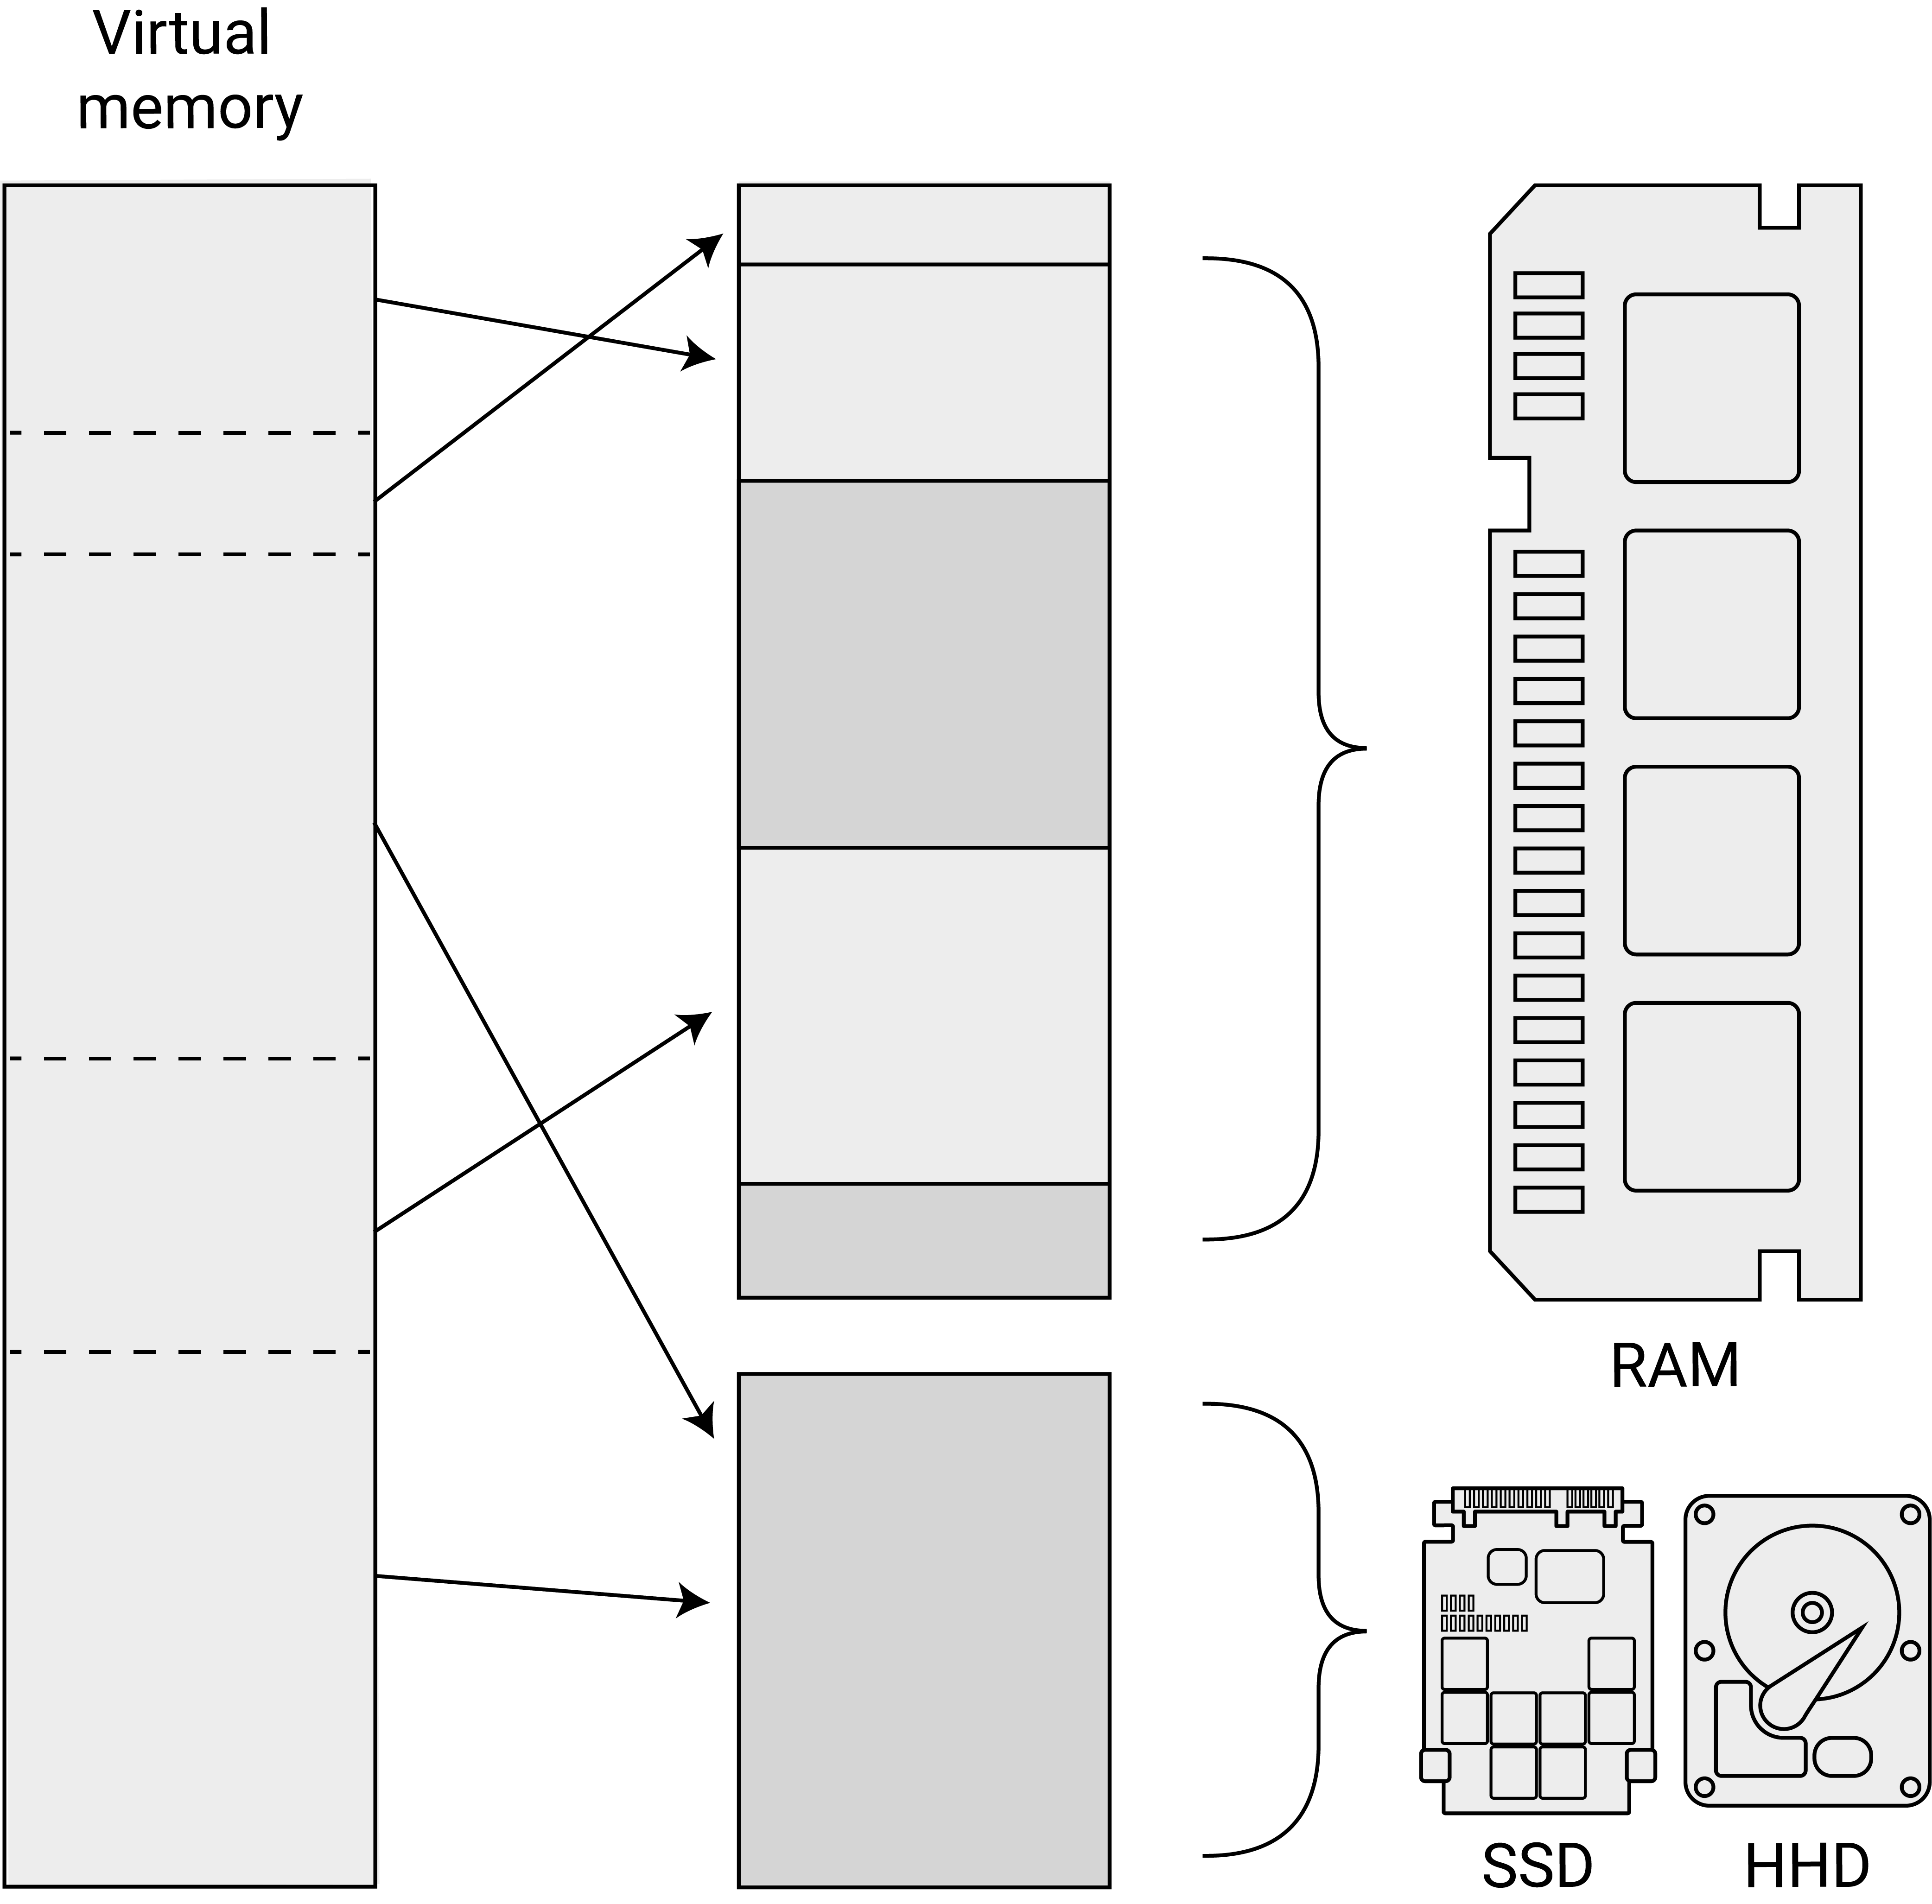
\includegraphics[width=0.75\linewidth]{img/virtual_memory} 

}

\caption{Virtual memory. Overall memory is mapped to RAM and parts of the hard disk.}\label{fig:vm}
\end{figure}



For example, when we implement an R-script that imports one file after the other into the R environment, ignoring the RAM capacity of our computer, the OS will start \emph{paging} data to the virtual memory. This happens `under the hood' without explicit instructions by the user. We will quite likely notice that the computer slows down a lot when this happens.

While this default usage of virtual memory by the OS is helpful for running several applications at the same time, each taking up a moderate amount of memory, it is not a really useful tool for processing large amounts of data in one application (R). However, the underlying idea of using both RAM and mass storage simultaneously in order to cope with a lack of memory is very useful in the context of Big Data analytics.

Several R packages have been developed that exploit the idea behind virtual memory explicitly for analyzing large amounts of data. The basic idea behind these packages is to map a dataset to the hard disk when loading it into R. The actual data values are stored in chunks on the hard disk, while the structure/metadata of the dataset is loaded into R.

\hypertarget{cpu-and-parallelization}{%
\section{CPU and parallelization}\label{cpu-and-parallelization}}

The actual processing of the data is done in the computer's central processing unit (CPU). Consequently, the performance of the CPU has a substantial effect on how fast a data analytics task runs. A CPU's performance is usually denoted by its \emph{clock rate} measured in gigaherz (GHz). In simple terms, a CPU with a clock rate of 4.8 GHz can execute 4.8 billion basic operations per second. Holding all other aspects constant, you can thus expect an analytics task to run faster if it runs on a computer with higher CPU clock rate. Alternatively to scaling up the CPU, we can exploit the fact that modern CPUs have several \emph{cores}. In the normal usage of a PC, the operating system makes use of these cores to run several applications smoothly \emph{in parallel} (e.g., you listen to music on Spotify while browsing the web and running some analytics script in RStudio in the background).

Modern computing environments such as R allow us to explicitly run parts of the same analytics task in parallel, that is, on several CPU cores at the same time. Following the same logic, we can also connect several computers (each with several CPU cores) in a cluster computer and run the program in parallel on all of these computing nodes. Both of these approaches are generally referred to as \emph{parallelization} and both are supported in several R packages.

An R program run in parallel typically involves the following steps

\begin{itemize}
\tightlist
\item
  First, several instances of R are running at the same time (across one machine with multiple CPU cores or across a cluster computer). One of the instances (i.e., the \emph{master} instance) breaks the computation into batches and sends those to the other instances.
\item
  Second, each of the instances processes its batch and sends the results back to the master instance.
\item
  Finally, the master instance combines the partial results into the final result and returns it to the user.
\end{itemize}

To illustrate this point, consider the following econometric problem: you have a customer \href{https://www.kaggle.com/jackdaoud/marketing-data?select=marketing_data.csv}{dataset} with detailed data on customer characteristics, past customer behavior, and information on online marketing campaigns. Your task is to figure out which customers are more likely to react positively to the most recent online marketing campaign. The aim is to optimize personalized marketing campaigns in the future based on insights gained from this exercise. In a first step you take a computationally intense ``brute force'' approach: you run all possible regressions with the dependent variable \texttt{Response} (equal to 1 if the customer took the offer in the campaign and 0 otherwise). In total you have 21 independent variables, thus you need to run \(2^20=1,048,576\) logit regressions (this is without considering linear combinations of covariates etc.). Finally, you want to select the model with the best fit according to deviance.

A simple sequential implementation to solve this problem could look like this (for the sake of time, we cap the number of regression models to N=10).

\begin{Shaded}
\begin{Highlighting}[]
\CommentTok{\# you can download the dataset from }
\CommentTok{\# https://www.kaggle.com/jackdaoud/marketing{-}data?}
\CommentTok{\# select=marketing\_data.csv}

\CommentTok{\# PREPARATION {-}{-}{-}{-}{-}{-}{-}{-}{-}{-}{-}{-}{-}{-}{-}{-}{-}{-}{-}{-}{-}{-}{-}{-}{-}{-}{-}{-}{-}}

\CommentTok{\# packages}
\FunctionTok{library}\NormalTok{(stringr)}

\CommentTok{\# import data}
\NormalTok{marketing }\OtherTok{\textless{}{-}} \FunctionTok{read.csv}\NormalTok{(}\StringTok{"data/marketing\_data.csv"}\NormalTok{)}
\CommentTok{\# clean/prepare data}
\NormalTok{marketing}\SpecialCharTok{$}\NormalTok{Income }\OtherTok{\textless{}{-}} \FunctionTok{as.numeric}\NormalTok{(}\FunctionTok{gsub}\NormalTok{(}\StringTok{"[[:punct:]]"}\NormalTok{,}
                                    \StringTok{""}\NormalTok{,}
\NormalTok{                                    marketing}\SpecialCharTok{$}\NormalTok{Income)) }
\NormalTok{marketing}\SpecialCharTok{$}\NormalTok{days\_customer }\OtherTok{\textless{}{-}} 
     \FunctionTok{as.Date}\NormalTok{(}\FunctionTok{Sys.Date}\NormalTok{())}\SpecialCharTok{{-}} 
     \FunctionTok{as.Date}\NormalTok{(marketing}\SpecialCharTok{$}\NormalTok{Dt\_Customer, }\StringTok{"\%m/\%d/\%y"}\NormalTok{)}
\NormalTok{marketing}\SpecialCharTok{$}\NormalTok{Dt\_Customer }\OtherTok{\textless{}{-}} \ConstantTok{NULL}

\CommentTok{\# all sets of independent vars}
\NormalTok{indep }\OtherTok{\textless{}{-}} \FunctionTok{names}\NormalTok{(marketing)[ }\FunctionTok{c}\NormalTok{(}\DecValTok{2}\SpecialCharTok{:}\DecValTok{19}\NormalTok{, }\DecValTok{27}\NormalTok{,}\DecValTok{28}\NormalTok{)]}
\NormalTok{combinations\_list }\OtherTok{\textless{}{-}} \FunctionTok{lapply}\NormalTok{(}\DecValTok{1}\SpecialCharTok{:}\FunctionTok{length}\NormalTok{(indep),}
                            \ControlFlowTok{function}\NormalTok{(x) }\FunctionTok{combn}\NormalTok{(indep, x,}
                                              \AttributeTok{simplify =} \ConstantTok{FALSE}\NormalTok{))}
\NormalTok{combinations\_list }\OtherTok{\textless{}{-}} \FunctionTok{unlist}\NormalTok{(combinations\_list, }
                            \AttributeTok{recursive =} \ConstantTok{FALSE}\NormalTok{)}
\NormalTok{models }\OtherTok{\textless{}{-}} \FunctionTok{lapply}\NormalTok{(combinations\_list,}
                 \ControlFlowTok{function}\NormalTok{(x) }\FunctionTok{paste}\NormalTok{(}\StringTok{"Response \textasciitilde{}"}\NormalTok{, }
                                   \FunctionTok{paste}\NormalTok{(x, }\AttributeTok{collapse=}\StringTok{"+"}\NormalTok{)))}

\CommentTok{\# COMPUTE REGRESSIONS {-}{-}{-}{-}{-}{-}{-}{-}{-}{-}{-}{-}{-}{-}{-}{-}{-}{-}{-}{-}{-}{-}{-}{-}{-}{-}}

\NormalTok{N }\OtherTok{\textless{}{-}} \DecValTok{10} \CommentTok{\#  N \textless{}{-} length(models) for all}
\NormalTok{pseudo\_Rsq }\OtherTok{\textless{}{-}} \FunctionTok{list}\NormalTok{()}
\FunctionTok{length}\NormalTok{(pseudo\_Rsq) }\OtherTok{\textless{}{-}}\NormalTok{ N}
\ControlFlowTok{for}\NormalTok{ (i }\ControlFlowTok{in} \DecValTok{1}\SpecialCharTok{:}\NormalTok{N) \{}
  \CommentTok{\# fit the logit model via maximum likelihood}
\NormalTok{  fit }\OtherTok{\textless{}{-}} \FunctionTok{glm}\NormalTok{(models[[i]], }\AttributeTok{data=}\NormalTok{marketing, }\AttributeTok{family =} \FunctionTok{binomial}\NormalTok{())}
  \CommentTok{\# compute the proportion of deviance explained by }
  \CommentTok{\# the independent vars (\textasciitilde{}R\^{}2)}
\NormalTok{  pseudo\_Rsq[[i]] }\OtherTok{\textless{}{-}} \DecValTok{1}\SpecialCharTok{{-}}\NormalTok{(fit}\SpecialCharTok{$}\NormalTok{deviance}\SpecialCharTok{/}\NormalTok{fit}\SpecialCharTok{$}\NormalTok{null.deviance)}
\NormalTok{\}}

\CommentTok{\# SELECT THE WINNER {-}{-}{-}{-}{-}{-}{-}{-}{-}{-}{-}{-}{-}{-}{-}}
\NormalTok{models[[}\FunctionTok{which.max}\NormalTok{(pseudo\_Rsq)]]}
\end{Highlighting}
\end{Shaded}

\begin{verbatim}
## [1] "Response ~ MntWines"
\end{verbatim}

\hypertarget{naive-multi-session-approach}{%
\subsection{Naive multi-session approach}\label{naive-multi-session-approach}}

There is actually a simple way of doing this ``manually'' on a multi-core PC, which intuitively illustrates the point of parallelization (although it would not be a very practical approach): you write an R script that loads the dataset, runs the fist \(n\) of the total of \(N\) regressions and stores the result in a local text file. Next, you run the script in your current RStudio session, open an additional RStudio session and run the script with the next \(n\) regressions, and so on until all cores are occupied with one RStudio session. At the end you collect all of the results from the separate text files and combine them to get the final result. Depending on the problem at hand, this could indeed speed up the overall task, and it is technically speaking a form of ``multi-session'' approach. However, as you have surely noticed, this is unlikely to be a very practical approach.

\hypertarget{multi-core-and-multi-node-approach}{%
\subsection{Multi-core and multi-node approach}\label{multi-core-and-multi-node-approach}}

A more practical approach is to write one R script (with the help of some specialized packages) that instructs R to automatically distribute the batches to different cores (or different computing nodes in a cluster computer), control and monitor the progress in all cores, and then automatically collect and combine the results from all cores. There are several approaches to achieve this in R.

\hypertarget{parallel-for-loops-using-socket}{%
\subsubsection{Parallel for-loops using socket}\label{parallel-for-loops-using-socket}}

Likely the most intuitive approach to parallelizing a task in R is the \texttt{foreach} package. It allows you to write a \texttt{foreach} statement that is very similar to the for-loop syntax in R. Hence, you can straightforwardly ``translate'' an already implemented sequential approach with a common for-loop to a parallel implementation.

\begin{Shaded}
\begin{Highlighting}[]
\CommentTok{\# COMPUTE REGRESSIONS IN PARALLEL (MULTI{-}CORE) {-}{-}{-}{-}{-}{-}{-}{-}{-}{-}{-}{-}{-}{-}{-}{-}{-}{-}{-}{-}{-}{-}{-}{-}{-}{-}}

\CommentTok{\# packages for parallel processing}
\FunctionTok{library}\NormalTok{(parallel)}
\FunctionTok{library}\NormalTok{(doSNOW)}

\CommentTok{\# get the number of cores available}
\NormalTok{ncores }\OtherTok{\textless{}{-}}\NormalTok{ parallel}\SpecialCharTok{::}\FunctionTok{detectCores}\NormalTok{()}
\CommentTok{\# set cores for parallel processing}
\NormalTok{ctemp }\OtherTok{\textless{}{-}} \FunctionTok{makeCluster}\NormalTok{(ncores)}
\FunctionTok{registerDoSNOW}\NormalTok{(ctemp)}

\CommentTok{\# prepare loop}
\NormalTok{N }\OtherTok{\textless{}{-}} \DecValTok{10000} \CommentTok{\#  N \textless{}{-} length(models) for all}
\CommentTok{\# run loop in parallel}
\NormalTok{pseudo\_Rsq }\OtherTok{\textless{}{-}}
  \FunctionTok{foreach}\NormalTok{ ( }\AttributeTok{i =} \DecValTok{1}\SpecialCharTok{:}\NormalTok{N, }\AttributeTok{.combine =}\NormalTok{ c) }\SpecialCharTok{\%dopar\%}\NormalTok{ \{}
    \CommentTok{\# fit the logit model via maximum likelihood}
\NormalTok{    fit }\OtherTok{\textless{}{-}} \FunctionTok{glm}\NormalTok{(models[[i]], }
               \AttributeTok{data=}\NormalTok{marketing,}
               \AttributeTok{family =} \FunctionTok{binomial}\NormalTok{())}
    \CommentTok{\# compute the proportion of deviance explained by }
    \CommentTok{\# the independent vars (\textasciitilde{}R\^{}2)}
    \FunctionTok{return}\NormalTok{(}\DecValTok{1}\SpecialCharTok{{-}}\NormalTok{(fit}\SpecialCharTok{$}\NormalTok{deviance}\SpecialCharTok{/}\NormalTok{fit}\SpecialCharTok{$}\NormalTok{null.deviance))}
\NormalTok{\}}

\CommentTok{\# SELECT THE WINNER {-}{-}{-}{-}{-}{-}{-}{-}{-}{-}{-}{-}{-}{-}{-}}
\NormalTok{models[[}\FunctionTok{which.max}\NormalTok{(pseudo\_Rsq)]]}
\end{Highlighting}
\end{Shaded}

\begin{verbatim}
## [1] "Response ~ Year_Birth+Teenhome+Recency+MntWines+days_customer"
\end{verbatim}

With relatively few cases, this approach is not very fast due to the overhead of ``distributing'' variables/objects from the master process to all cores/workers. In simple terms, the socket approach means that the cores do not share the same variables/the same environment, which creates overhead. However, this approach is usually very stable and runs on all platforms.

\hypertarget{parallel-lapply-using-forking}{%
\subsubsection{Parallel lapply using forking}\label{parallel-lapply-using-forking}}

Finally, let us look at the implementation based on forking. In the fork approach, each core works with the same objects/variables in a shared environment, which makes this approach very fast. However, depending on what exactly is being computed, sharing an environment can cause problems.\footnote{Also, this approach does not work on Windows machines (see \texttt{?mclapply} for details).} If you are not sure whether your set up might run into issues with forking, it would be better to rely on a non-fork approach.

\begin{Shaded}
\begin{Highlighting}[]
\CommentTok{\# COMPUTE REGRESSIONS IN PARALLEL (MULTI{-}CORE) {-}{-}{-}{-}{-}{-}{-}{-}{-}{-}{-}{-}{-}{-}{-}}


\CommentTok{\# prepare parallel lapply (based on forking, }
\CommentTok{\# here clearly faster than foreach)}
\NormalTok{N }\OtherTok{\textless{}{-}} \DecValTok{10000} \CommentTok{\#  N \textless{}{-} length(models) for all}
\CommentTok{\# run parallel lapply}
\NormalTok{pseudo\_Rsq }\OtherTok{\textless{}{-}} \FunctionTok{mclapply}\NormalTok{(}\DecValTok{1}\SpecialCharTok{:}\NormalTok{N,}
                       \AttributeTok{mc.cores =}\NormalTok{ ncores,}
                       \AttributeTok{FUN =} \ControlFlowTok{function}\NormalTok{(i)\{}
                         \CommentTok{\# fit the logit model }
\NormalTok{                         fit }\OtherTok{\textless{}{-}} \FunctionTok{glm}\NormalTok{(models[[i]],}
                                    \AttributeTok{data=}\NormalTok{marketing,}
                                    \AttributeTok{family =} \FunctionTok{binomial}\NormalTok{())}
                         \CommentTok{\# compute the proportion of deviance }
                         \CommentTok{\# explained  by the independent vars (\textasciitilde{}R\^{}2)}
                         \FunctionTok{return}\NormalTok{(}\DecValTok{1}\SpecialCharTok{{-}}\NormalTok{(fit}\SpecialCharTok{$}\NormalTok{deviance}\SpecialCharTok{/}\NormalTok{fit}\SpecialCharTok{$}\NormalTok{null.deviance))}
\NormalTok{                         \})}

\CommentTok{\# SELECT THE WINNER, SHOW FINAL OUTPUT {-}{-}{-}{-}{-}{-}{-}{-}{-}{-}{-}{-}{-}{-}{-}}

\NormalTok{best\_model }\OtherTok{\textless{}{-}}\NormalTok{ models[[}\FunctionTok{which.max}\NormalTok{(pseudo\_Rsq)]]}
\NormalTok{best\_model}
\end{Highlighting}
\end{Shaded}

\begin{verbatim}
## [1] "Response ~ Year_Birth+Teenhome+Recency+MntWines+days_customer"
\end{verbatim}

\hypertarget{gpus-for-scientific-computing}{%
\section{GPUs for scientific computing}\label{gpus-for-scientific-computing}}

The success of the computer games industry in the late 1990s/early 2000s led to an interesting positive externality for scientific computing. The ever more demanding graphics of modern computer games and the huge economic success of the computer games industry set incentives for hardware producers to invest in research and development of more powerful `graphic cards', extending a normal PC/computing environment with additional computing power solely dedicated to graphics. At the heart of these graphic cards are so-called GPUs (graphic processing units), microprocessors specifically optimized for graphics processing. Figure 4.3 depicts a modern graphics card similar to those commonly built into today's `gaming' PCs.

\begin{figure}

{\centering 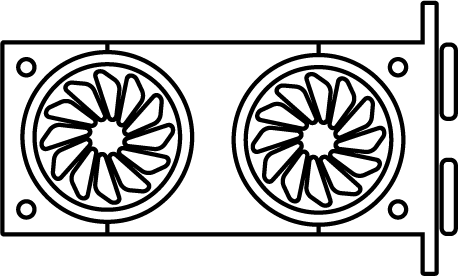
\includegraphics[width=0.4\linewidth]{img/GPU} 

}

\caption{Illustration of a graphic processing unit (GPU).}\label{fig:gpu}
\end{figure}



Why did the hardware industry not simply invest in the development of more powerful CPUs to deal with the more demanding PC games? The main reason is that the architecture of CPUs is designed not only for efficiency but also flexibility. That is, a CPU needs to perform well in all kinds of computations, some parallel, some sequential, etc. Computing graphics is a comparatively narrow domain of computation, and designing a processing unit architecture that is custom-made to excel just at this one task is thus much more cost efficient. Interestingly, this graphics-specific architecture (specialized in highly parallel numerical {[}floating point{]} workloads) turns out to also be very useful in some core scientific computing tasks -- in particular, matrix multiplications (see \citet{fatahalian_etal2004} for a detailed discussion of why that is the case). A key aspect of GPUs is that they are composed of several multiprocessor units, of which each in turn has several cores. GPUs can thus perform computations with hundreds or even thousands of threads in parallel. The figure below illustrates this point by showing the typical architecture of a NVIDIA GPU.

\begin{figure}

{\centering \includegraphics[width=0.95\linewidth]{img/gpu_details} 

}

\caption{Illustration of a graphic processing unit (GPU).}\label{fig:gpuarchitecture}
\end{figure}



While, initially, programming GPUs for scientific computing required a very good understanding of the hardware, graphics card producers have realized that there is an additional market for their products (in particular with the recent rise of deep learning) and now provide several high-level APIs to use GPUs for tasks other than graphics processing. Over the last few years, more high-level software has been developed that makes it much easier to use GPUs in parallel computing tasks. The following subsections show some examples of such software in the R environment.\footnote{Note that while these examples are easy to implement and run, setting up a GPU for scientific computing still can involve many steps and some knowledge of your computer's system. The examples presuppose that all installation and configuration steps (GPU drivers, CUDA, etc.) have already been completed successfully.}

\hypertarget{gpus-in-r}{%
\subsection{GPUs in R}\label{gpus-in-r}}

\hypertarget{gpu-computing-example-matrix-multiplication-comparison-gpur}{%
\subsubsection{\texorpdfstring{GPU computing example: Matrix multiplication comparison (\texttt{gpuR})}{GPU computing example: Matrix multiplication comparison (gpuR)}}\label{gpu-computing-example-matrix-multiplication-comparison-gpur}}

The \texttt{gpuR} package provides basic R functions to compute with GPUs from within the R environment. In the following example we compare the performance of a CPU with a GPU based on a matrix multiplication exercise. For a large \(N\times P\) matrix \(X\), we want to compute \(X^tX\).

In a first step, we load the \texttt{gpuR}-package.\footnote{As with setting up GPUs on your machine in general, installing all prerequisites to make \texttt{gpuR} work on your local machine can be a bit of work and can depend a lot on your system.} Note the output to the console. It shows the type of GPU identified by \texttt{gpuR}. This is the platform on which \texttt{gpuR} will compute the GPU examples. In order to compare the performances, we also load the \texttt{bench} package.

\begin{Shaded}
\begin{Highlighting}[]
\CommentTok{\# load package}
\FunctionTok{library}\NormalTok{(bench)}
\FunctionTok{library}\NormalTok{(gpuR)}
\end{Highlighting}
\end{Shaded}

\begin{verbatim}
## Number of platforms: 1
## - platform: NVIDIA Corporation: OpenCL 3.0 CUDA 11.6.134
##   - context device index: 0
##     - NVIDIA GeForce GTX 1650
## checked all devices
## completed initialization
\end{verbatim}

Next, we initialize a large matrix filled with pseudo-random numbers, representing a dataset with \(N\) observations and \(P\) variables.

\begin{Shaded}
\begin{Highlighting}[]
\CommentTok{\# initialize dataset with pseudo{-}random numbers}
\NormalTok{N }\OtherTok{\textless{}{-}} \DecValTok{10000}  \CommentTok{\# number of observations}
\NormalTok{P }\OtherTok{\textless{}{-}} \DecValTok{100} \CommentTok{\# number of variables}
\NormalTok{X }\OtherTok{\textless{}{-}} \FunctionTok{matrix}\NormalTok{(}\FunctionTok{rnorm}\NormalTok{(N }\SpecialCharTok{*}\NormalTok{ P, }\DecValTok{0}\NormalTok{, }\DecValTok{1}\NormalTok{), }\AttributeTok{nrow =}\NormalTok{ N, }\AttributeTok{ncol =}\NormalTok{P)}
\end{Highlighting}
\end{Shaded}

For the GPU examples to work, we need one more preparatory step. GPUs have their own memory, which they can access faster than they can access RAM. However, this GPU memory is typically not very large compared to the memory CPUs have access to. Hence, there is a potential trade-off between losing some efficiency but working with more data or vice versa.\footnote{If we instruct the GPU to use its own memory but the data does not fit in it, the program will result in an error.} Here, we show both variants. With \texttt{gpuMatrix()} we create an object representing matrix \texttt{X} for computation on the GPU. However, this only points the GPU to the matrix and does not actually transfer data to the GPU's memory. The latter is done in the other variant, with \texttt{vclMatrix()}.

\begin{Shaded}
\begin{Highlighting}[]
\CommentTok{\# prepare GPU{-}specific objects/settings}

\CommentTok{\# point GPU to matrix (matrix stored in non{-}GPU memory)}
\NormalTok{gpuX }\OtherTok{\textless{}{-}} \FunctionTok{gpuMatrix}\NormalTok{(X, }\AttributeTok{type =} \StringTok{"float"}\NormalTok{)}
\CommentTok{\# transfer matrix to GPU (matrix stored in GPU memory)}
\NormalTok{vclX }\OtherTok{\textless{}{-}} \FunctionTok{vclMatrix}\NormalTok{(X, }\AttributeTok{type =} \StringTok{"float"}\NormalTok{)  }
\end{Highlighting}
\end{Shaded}

Now we run the three examples: first, based on standard R, using the CPU. Then, computing on the GPU but using CPU memory. And finally, computing on the GPU and using GPU memory. In order to make the comparison fair, we force \texttt{bench::mark()} to run at least 20 iterations per benchmarked variant.

\begin{Shaded}
\begin{Highlighting}[]
\CommentTok{\# compare three approaches}
\NormalTok{(gpu\_cpu }\OtherTok{\textless{}{-}}\NormalTok{ bench}\SpecialCharTok{::}\FunctionTok{mark}\NormalTok{(}
  
  \CommentTok{\# compute with CPU }
\NormalTok{  cpu }\OtherTok{\textless{}{-}} \FunctionTok{t}\NormalTok{(X) }\SpecialCharTok{\%*\%}\NormalTok{ X,}
  
  \CommentTok{\# GPU version, GPU pointer to CPU memory }
  \CommentTok{\# (gpuMatrix is simply a pointer)}
\NormalTok{  gpu1\_pointer }\OtherTok{\textless{}{-}} \FunctionTok{t}\NormalTok{(gpuX) }\SpecialCharTok{\%*\%}\NormalTok{ gpuX,}
  
  \CommentTok{\# GPU version, in GPU memory }
  \CommentTok{\# (vclMatrix formation is a memory transfer)}
\NormalTok{  gpu2\_memory }\OtherTok{\textless{}{-}} \FunctionTok{t}\NormalTok{(vclX) }\SpecialCharTok{\%*\%}\NormalTok{ vclX,}
 
\AttributeTok{check =} \ConstantTok{FALSE}\NormalTok{, }\AttributeTok{memory =} \ConstantTok{FALSE}\NormalTok{, }\AttributeTok{min\_iterations =} \DecValTok{20}\NormalTok{))}
\end{Highlighting}
\end{Shaded}

\begin{verbatim}
## # A tibble: 3 x 6
##   expression                            min   median
##   <bch:expr>                       <bch:tm> <bch:tm>
## 1 cpu <- t(X) %*% X                  76.8ms   77.7ms
## 2 gpu1_pointer <- t(gpuX) %*% gpuX  32.21ms     34ms
## 3 gpu2_memory <- t(vclX) %*% vclX    9.36ms   15.1ms
## # ... with 3 more variables: `itr/sec` <dbl>,
## #   mem_alloc <bch:byt>, `gc/sec` <dbl>
## # i Use `colnames()` to see all variable names
\end{verbatim}

The performance comparison is visualized with boxplots.

\begin{Shaded}
\begin{Highlighting}[]
\FunctionTok{plot}\NormalTok{(gpu\_cpu, }\AttributeTok{type =} \StringTok{"boxplot"}\NormalTok{)}
\end{Highlighting}
\end{Shaded}

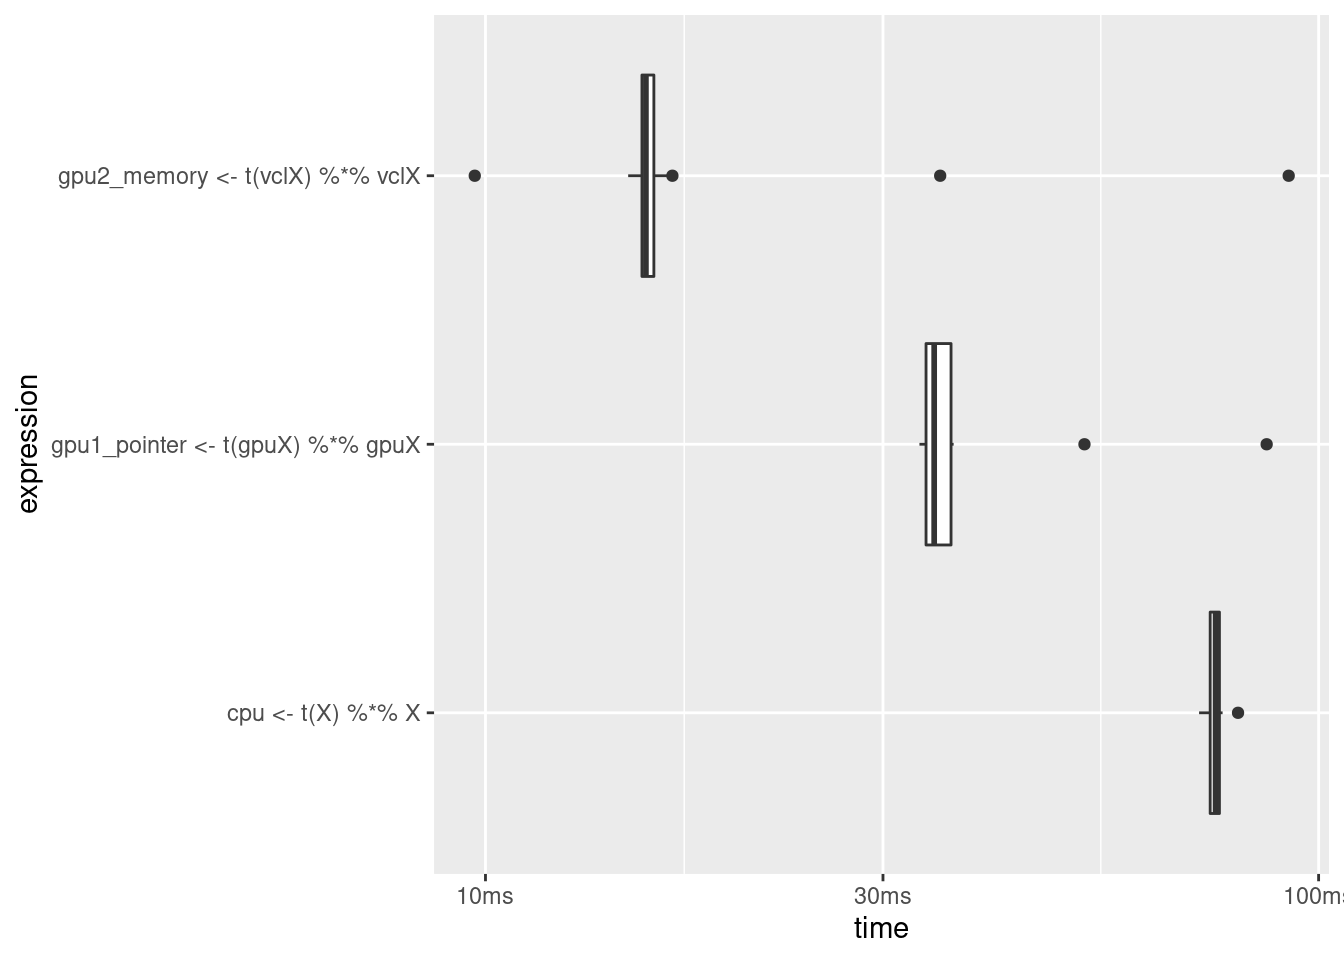
\includegraphics{bigdata_files/figure-latex/unnamed-chunk-78-1.pdf}

The theoretically expected pattern becomes clearly visible. When using the GPU + GPU memory, the matrix operation takes on average less than 20 ms, with GPU + RAM over 30 ms, and with the common CPU operation close to 100 ms to finish. In the chapters on applied data analysis, we will look at some applications of GPUs in the domain of deep learning (which relies heavily on matrix multiplications).

\hypertarget{the-road-ahead-hardware-made-for-machine-learning}{%
\section{The road ahead: Hardware made for machine learning}\label{the-road-ahead-hardware-made-for-machine-learning}}

Due to the high demand for more computational power in the domain of training complex neural network models (for example, in computer vision), Google has recently developed a new hardware platform specifically designed to work with complex neural networks using TensorFlow: Tensor Processing Units (TPUs). TPUs were designed from the ground up to improve performance in dense vector and matrix computations with the aim of substantially increasing the speed of training deep learning models implemented with TensorFlow.

\begin{figure}

{\centering 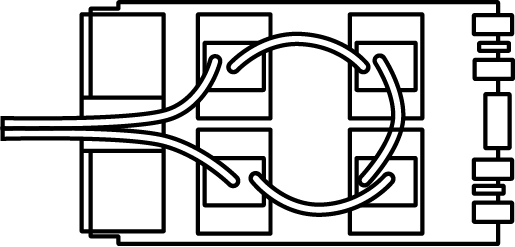
\includegraphics[width=0.4\linewidth]{img/TPU} 

}

\caption{Illustration of a tensor processing unit (GPU).}\label{fig:tpu}
\end{figure}



While initially only used internally by Google, the Google Cloud platform now offers cloud TPUs to the general public.

\hypertarget{insufficient-computing-resources}{%
\section{Insufficient computing resources?}\label{insufficient-computing-resources}}

When working with very large datasets (i.e., terabytes of data), processing the data on one common computer might not work due to a lack of memory or would be way too slow due to a lack of computing power (CPU cores). The architecture or basic hardware set up of a common computer is subject to a limited amount of RAM and a limited number of CPUs/CPU cores. Hence simply scaling up might not be sufficient. Instead we need to scale out. In simple terms, this means connecting several computers (each with their own RAM, CPU, and mass storage) in a network, distributing the dataset across all computers (``nodes'') in this network, and working on the data simultaneously across all nodes. In the next chapter, we look into how such ``distributed systems'\,' basically work, what software frameworks are commonly used to work on distributed systems, and how we can interact with this software (and the distributed system) via R and SQL.

\hypertarget{distributed-systems}{%
\chapter{Distributed Systems}\label{distributed-systems}}

When we connect several computers in a network to jointly process large amounts of data, such a computing system is commonly referred to as a ``distributed system''. From a technical standpoint the key difference between a distributed system and the more familiar parallel system (e.g.~our desktop computer with its multicore CPU) is that in distributed systems the different components do not share the same memory (and storage). Figure \ref{fig:distributedsystems} illustrates this point.

\begin{figure}

{\centering 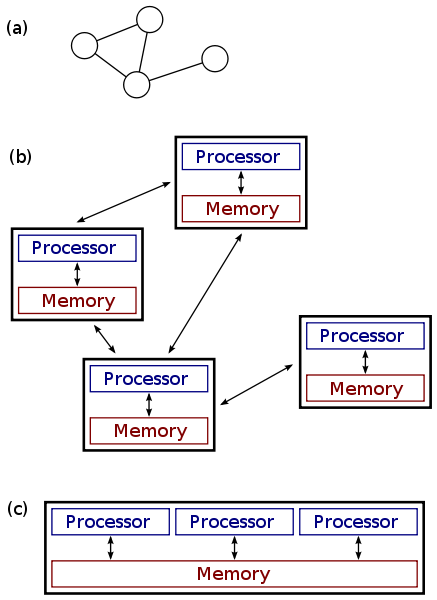
\includegraphics[width=0.3\linewidth]{img/distributed_systems} 

}

\caption{(a), (b): a distributed system. (c): a parallel system.I llustration by Miym (CC BY-SA 3.0).}\label{fig:distributedsystems}
\end{figure}



In a distributed system, the data set is literally split up into pieces that then reside separately on different nodes. This requires an additional ``layer'' of software (that coordinates the distribution/loading of data as well as the simultaneous processing) and a different approach (a different ``programming model'') to defining computing/data analytics tasks. Below, we will look at both of these aspects in turn.

\hypertarget{mapreduce}{%
\section{MapReduce}\label{mapreduce}}

The most broadly used programming model and its implementation for processing big data on distributed systems is called MapReduce. It essentially consists of two procedures and is conceptually very close to the ``split-apply-combine'' strategy in data analysis. First, the Map function sorts/filters the data (on each node). Then, a Reduce function aggregates the sorted/filtered data. In the background, the MapReduce ``framework'' orchestrates these processes across all nodes, collects the results, and returns them to the user.

Let us illustrate the basic idea behind MapReduce with a simple example. Suppose you are working on a text mining task in which all the raw text in thousands of digitized books (stored as text files) need to be processed. In a first step, you want to compute word frequencies (countthe number of occurrences of specific words in all books combined).

For simplicity, let us only focus on the following excerpts from two exemplary (and rather cryptic) books on botany:

Text in book 1:

\emph{Apple Orange Mango}
~

\emph{Orange Grapes Plum}
~

Text in book 2:

\emph{Apple Plum Mango}
~

\emph{Apple Apple Plum}
~

The figure below illustrates the MapReduce process. First, the data is loaded from the original text files. Each line of text is then passed to individual mapper instances which separately split the lines of text into key-value pairs. Then the system sorts and shuffles all key-value pairs across all instances and finally. The reducer aggregates the sorted/shuffled key-value pairs (here: counts the number of word occurrences) and, finally, the master instance collects all the results and returns the final output. From this simple example, a key aspect of MapReduce should become clear: for the key tasks of mapping and reducing the data processing on one node/instance can happen completely independent from the processing on the other instances. Note that not for every data anlytics task this is so easily conceivable as for computing word frequencies.

\begin{figure}

{\centering 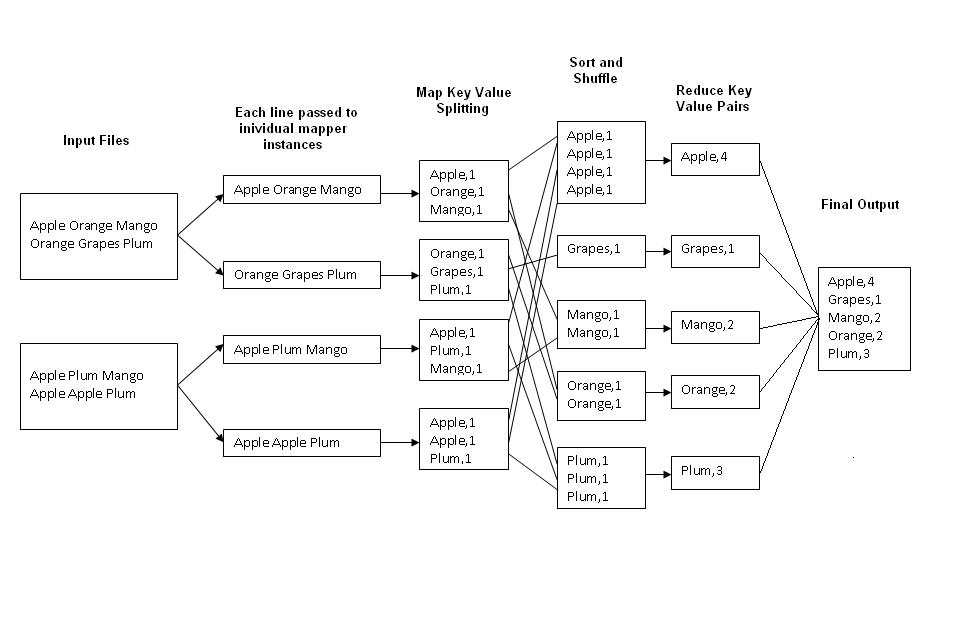
\includegraphics[width=0.9\linewidth]{img/mapreduce_wordcount} 

}

\caption{Illustration of the MapReduce programming model.}\label{fig:mapreduce}
\end{figure}



\hypertarget{mapreduce-concept-illustrated-in-r}{%
\subsection{Map/Reduce Concept Illustrated in R}\label{mapreduce-concept-illustrated-in-r}}

In order to better understand the basic concept behind the MapReduce-Framework on a distributed system, let's look at how we can combine the functions \texttt{map()} and \texttt{reduce()} in R to implement the basic MapReduce example shown above (this is just to illustrate the underlying idea, \emph{not} to suggest that MapReduce actually is simply an application of the classical \texttt{map} and \texttt{reduce\ (fold)} functions in functional programming).\footnote{For a more detailed discussion of what \texttt{map} and \texttt{reduce} have \emph{actually} to do with MapReduce see \href{https://medium.com/@jkff/mapreduce-is-not-functional-programming-39109a4ba7b2}{this post}.} The overall aim of the program is to count the number of times each word is repeated in a given text. The input to the program is thus a text, the output is a list of key-value pairs with the unique words occurring in the text as keys and their respective number of occurrences as values.

In the code example, we will use the following text as input.

\begin{Shaded}
\begin{Highlighting}[]
\CommentTok{\# initiate the input text (for simplicity as one text string)}

\NormalTok{input\_text }\OtherTok{\textless{}{-}}

\StringTok{"Apple Orange Mango}
\StringTok{Orange Grapes Plum}
\StringTok{Apple Plum Mango}
\StringTok{Apple Apple Plum"}
\end{Highlighting}
\end{Shaded}

\hypertarget{mapper}{%
\subsection{Mapper}\label{mapper}}

The Mapper first splits the text into lines, and then splits the lines into key-value pairs, assigning to each key the value \texttt{1}. For the first step we use \texttt{strsplit()} that takes a character string as input and splits it into a list of substrings according to the matches of a substring (here \texttt{"\textbackslash{}n"}, indicating the end of a line).

\begin{Shaded}
\begin{Highlighting}[]
\CommentTok{\# Mapper splits input into lines}
\NormalTok{lines }\OtherTok{\textless{}{-}} \FunctionTok{as.list}\NormalTok{(}\FunctionTok{strsplit}\NormalTok{(input\_text, }\StringTok{"}\SpecialCharTok{\textbackslash{}n}\StringTok{"}\NormalTok{)[[}\DecValTok{1}\NormalTok{]])}
\NormalTok{lines}
\end{Highlighting}
\end{Shaded}

\begin{verbatim}
## [[1]]
## [1] "Apple Orange Mango"
## 
## [[2]]
## [1] "Orange Grapes Plum"
## 
## [[3]]
## [1] "Apple Plum Mango"
## 
## [[4]]
## [1] "Apple Apple Plum"
\end{verbatim}

In a second step, we apply our own function (\texttt{map\_fun()}) to each line of text via \texttt{Map()}. \texttt{map\_fun()} splits each line into words (keys) and assigns a value of \texttt{1} to each key.

\begin{Shaded}
\begin{Highlighting}[]
\CommentTok{\# Mapper splits lines into Key{-}Value pairs}
\NormalTok{map\_fun }\OtherTok{\textless{}{-}}
     \ControlFlowTok{function}\NormalTok{(x)\{}
          
          \CommentTok{\# remove special characters}
\NormalTok{          x\_clean }\OtherTok{\textless{}{-}} \FunctionTok{gsub}\NormalTok{(}\StringTok{"[[:punct:]]"}\NormalTok{, }\StringTok{""}\NormalTok{, x)}
          \CommentTok{\# split line into words}
\NormalTok{          keys }\OtherTok{\textless{}{-}} \FunctionTok{unlist}\NormalTok{(}\FunctionTok{strsplit}\NormalTok{(x\_clean, }\StringTok{" "}\NormalTok{))}
          \CommentTok{\# initiate key{-}value pairs}
\NormalTok{          key\_values }\OtherTok{\textless{}{-}} \FunctionTok{rep}\NormalTok{(}\DecValTok{1}\NormalTok{, }\FunctionTok{length}\NormalTok{(keys))}
          \FunctionTok{names}\NormalTok{(key\_values) }\OtherTok{\textless{}{-}}\NormalTok{ keys}
          
          \FunctionTok{return}\NormalTok{(key\_values)}
\NormalTok{     \}}

\NormalTok{kv\_pairs }\OtherTok{\textless{}{-}} \FunctionTok{Map}\NormalTok{(map\_fun, lines)}

\CommentTok{\# look at the result}
\NormalTok{kv\_pairs}
\end{Highlighting}
\end{Shaded}

\begin{verbatim}
## [[1]]
##  Apple Orange  Mango 
##      1      1      1 
## 
## [[2]]
## Orange Grapes   Plum 
##      1      1      1 
## 
## [[3]]
## Apple  Plum Mango 
##     1     1     1 
## 
## [[4]]
## Apple Apple  Plum 
##     1     1     1
\end{verbatim}

\hypertarget{reducer}{%
\subsection{Reducer}\label{reducer}}

The Reducer first sorts and shuffles the input from the Mapper and then reduces the key-value pairs by summing up the values for each key.

\begin{Shaded}
\begin{Highlighting}[]
\CommentTok{\# order and shuffle}
\NormalTok{kv\_pairs }\OtherTok{\textless{}{-}} \FunctionTok{unlist}\NormalTok{(kv\_pairs)}
\NormalTok{keys }\OtherTok{\textless{}{-}} \FunctionTok{unique}\NormalTok{(}\FunctionTok{names}\NormalTok{(kv\_pairs))}
\NormalTok{keys }\OtherTok{\textless{}{-}}\NormalTok{ keys[}\FunctionTok{order}\NormalTok{(keys)]}
\NormalTok{shuffled }\OtherTok{\textless{}{-}} \FunctionTok{lapply}\NormalTok{(keys,}
                    \ControlFlowTok{function}\NormalTok{(x) kv\_pairs[x }\SpecialCharTok{==} \FunctionTok{names}\NormalTok{(kv\_pairs)])}
\NormalTok{shuffled}
\end{Highlighting}
\end{Shaded}

\begin{verbatim}
## [[1]]
## Apple Apple Apple Apple 
##     1     1     1     1 
## 
## [[2]]
## Grapes 
##      1 
## 
## [[3]]
## Mango Mango 
##     1     1 
## 
## [[4]]
## Orange Orange 
##      1      1 
## 
## [[5]]
## Plum Plum Plum 
##    1    1    1
\end{verbatim}

Now we can sum up the keys in order to get the word count for the entire input.

\begin{Shaded}
\begin{Highlighting}[]
\NormalTok{sums }\OtherTok{\textless{}{-}} \FunctionTok{lapply}\NormalTok{(shuffled, Reduce, }\AttributeTok{f=}\NormalTok{sum)}
\FunctionTok{names}\NormalTok{(sums) }\OtherTok{\textless{}{-}}\NormalTok{ keys}
\NormalTok{sums}
\end{Highlighting}
\end{Shaded}

\begin{verbatim}
## $Apple
## [1] 4
## 
## $Grapes
## [1] 1
## 
## $Mango
## [1] 2
## 
## $Orange
## [1] 2
## 
## $Plum
## [1] 3
\end{verbatim}

\hypertarget{hadoop}{%
\section{Hadoop}\label{hadoop}}

Hadoop is probably the most broadly known and used system to implement the MapReduce framework. A decade ago big data analytics with really large data sets often involved directly interacting with/ working in Hadoop to run MapReduce jobs. However, over the last few years various higher-level interfaces have been developed that make the usage of MapReduce/Hadoop for data analysts much more easily accessible. The purpose of this section is thus to give a lightweight introduction to the underlying basics that power some of the code examples and tutorials discussed in the data analytics chapters towards the end of this book.

\begin{center}
\includegraphics[width=0.9\linewidth]{img/hadoop} \end{center}

\hypertarget{hadoop-word-count-example}{%
\subsection{Hadoop word count example}\label{hadoop-word-count-example}}

To get an idea of how running a Hadoop job looks like, we run the same simple word count example introduced above on a local Hadoop installation. The example presupposes a local installation of Hadoop version 2.10.1 (see Appendix C for details) and can easily be run on a completely normal desktop/laptop computer running Ubuntu Linux. As a side remark, this actually illustrates an important aspect of developing MapReduce scripts in Hadoop (and many of the software packages building on it): the code can be easily developed tested locally on a small machine and only later transferred to the actual Hadoop cluster to be run on the full data set.

The basic Hadoop installation comes with a few templates for very typical map/reduce programs.\footnote{More sophisticated programs need to be custom made, written in Java.} Below we replicate the same word-count example as shown in simple R code above.

In a first step, we create an input directory where we store the input file(s) to feed to Hadoop.

\begin{Shaded}
\begin{Highlighting}[]
\CommentTok{\# create directory for input files (typically text files)}
\FunctionTok{mkdir}\NormalTok{ \textasciitilde{}/input}
\end{Highlighting}
\end{Shaded}

Then we add a text file containing the same text as in the example above.

\begin{Shaded}
\begin{Highlighting}[]
\BuiltInTok{echo} \StringTok{"Apple Orange Mango}
\StringTok{Orange Grapes Plum}
\StringTok{Apple Plum Mango}
\StringTok{Apple Apple Plum"} \OperatorTok{\textgreater{}\textgreater{}}\NormalTok{  \textasciitilde{}/input/text.txt}
\end{Highlighting}
\end{Shaded}

Now we can run the MapReduce/Hadoop word count as follows, storing the results in a new directory called \texttt{wordcount\_example}. This is where we use the already implemented Hadoop script to run a word count job Map/Reduce style. This is where we rely on the already implemented wordcount example provided with the Hadoop installation (located in \texttt{/usr/local/hadoop/share/hadoop/mapreduce/hadoop-mapreduce-examples-2.10.1.jar})

\begin{Shaded}
\begin{Highlighting}[]
\CommentTok{\# run mapreduce word count}
\ExtensionTok{/usr/local/hadoop/bin/hadoop}\NormalTok{ jar /usr/local/hadoop/share/hadoop/mapreduce/hadoop{-}mapreduce{-}examples{-}2.10.1.jar wordcount \textasciitilde{}/input \textasciitilde{}/wc\_example}
\end{Highlighting}
\end{Shaded}

What this line says is: run the Hadoop program called \texttt{wordcount} implemented in the jar-file \texttt{hadoop-mapreduce-examples-2.10.1.jar}, use the files in directory \texttt{\textasciitilde{}/input} containing the raw text as input and store the final output in directory \texttt{\textasciitilde{}/wc\_example}.

\begin{Shaded}
\begin{Highlighting}[]
\FunctionTok{cat}\NormalTok{ \textasciitilde{}/wc\_example/}\PreprocessorTok{*}
\end{Highlighting}
\end{Shaded}

\begin{verbatim}
## Apple    4
## Grapes   1
## Mango    2
## Orange   2
## Plum 3
\end{verbatim}

What looks rather simple in this example can get very complex once you want to write an entire data analysis script with all kind of analysis for Hadoop. Also, Hadoop was designed for batch processing and does not offer a simple interface for interactive sessions. All of this makes it rather impractical for a usual analytics workflow as we know it from working with R. This is where \href{https://spark.apache.org/}{Apache Spark} comes to the rescue.

\hypertarget{spark}{%
\section{Spark}\label{spark}}

Also building on the MapReduce model, Spark is a cluster computing platform particularly made for data analytics. It partially relies on Hadoop for handling storage and resource management, but offers way more easy-to-use high-level interfaces for typical analytics tasks. From the technical perspective (in very simple terms), Spark also addresses some shortcomings of the Hadoop platform, further improving efficiency/speed for many data analysis tasks. More importantly for our purposes, in contrast to Hadoop, Spark is specifically made for interactively developing and runnin data analytics scripts and therefore more easily accessible for people with an applied econometrics background but no substantial knowledge in MapReduce cluster computing. In particular, it comes with several high-level operators that make it rather easy to implement analytics tasks. Moreover, as we will see in later chapters, it is very easy to use interactively from within R (and other languages like Python, SQL, and Scala). This makes the platform much more accessible and worth the while for empirical economic research, even for relatively simple econometric analyses.

The following figure illustrates the basic components of Spark. The main functionality, including memory management, task scheduling, and the implementation of Spark's capabilities to handle and manipulate data distributed across many nodes in parallel. Several built-in libraries extend the core implementation, covering specific domains of practical data analytics tasks (querying structured data via SQL, processing streams of data, machine learning, and network/graph analysis). The latter two provide various common functions/algorithms frequently used in data analytics/applied econometrics, such as generalized linear regression, summary statistics, and principal component analysis.

\begin{figure}

{\centering 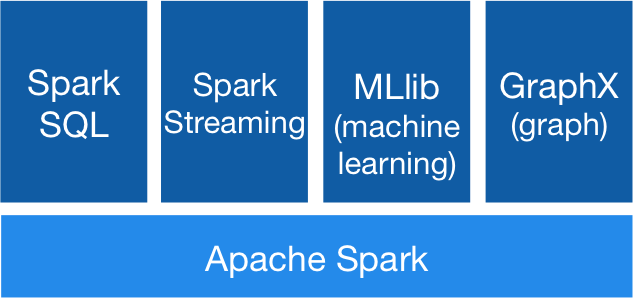
\includegraphics[width=0.6\linewidth]{img/spark-stack} 

}

\caption{Basic Spark stack (source: \url{https://spark.apache.org/images/spark-stack.png})}\label{fig:sparkstack}
\end{figure}



At the heart of big data analytics with Spark is the fundamental data structure called `resilient distributed data set' (RDD). When loading/importing data into Spark, the data is automatically distributed across the cluster in RDDs (\textasciitilde{} as distributed collections of elements) and manipulations are then executed in parallel in these RDDs. However, the entire Spark framework also works locally on a simple laptop or desktop computer. This is of great advantage when learning Spark and testing/debugging an analytics script on a small sample of the real data set.

\hypertarget{spark-with-r}{%
\section{Spark with R}\label{spark-with-r}}

There are two prominent packages to use Spark in connection to R: \texttt{SparkR} and RStudio's \texttt{sparklyr}, the former is in some ways closer to Spark's Python API, the latter is closer to the \texttt{dplyr}-type of data handling (and is `compatible' with the `\texttt{tidyverse}').\footnote{See \href{https://cosminsanda.com/posts/a-compelling-case-for-sparkr/}{this blog post} for a more detailed comparison and discussion of advantages of either package.} For the very simple introductory examples below, either package could have been used equally well. For the general introduction we focus on \texttt{SparkR} and later have a look at a simple regression example based on \texttt{sparklyr}.

To install and use Spark from the R shell, only a few preparatory steps are needed. The following examples are based on installing/running Spark on a Linux machine with the \texttt{SparkR} package. \texttt{SparkR} depends on Java (version 8). Thus, we first should make sure the right Java version is installed. If several Java versions are installed, we might have to select version 8 manually via the following terminal command (Linux).

With the right version of Java running, we can install \texttt{SparkR} from GitHub (needs the \texttt{devtools}-package) \texttt{devtools::install\_github("cran/SparkR")}. After installing \texttt{SparkR}, the call \texttt{SparkR::install.spark()} will download and install Apache Spark to a local directory.\footnote{Note that after the installation, the location of Spark is printed to the R console. Alternatively, you can also first install the \texttt{sparklyr}-package and then run \texttt{sparklyr::spark\_install()} to install Spark. In the data analysis examples later in the book we will work both with \texttt{SparkR} and \texttt{sparklyr}.} Now we can start an interactive SparkR session from the terminal with

\begin{Shaded}
\begin{Highlighting}[]
\ExtensionTok{$}\NormalTok{ SPARK{-}HOME/bin/sparkR}
\end{Highlighting}
\end{Shaded}

where \texttt{SPARK-HOME} is a placeholder for the path to your local Spark installation (printed to the console after running \texttt{SparkR::install.spark()}). Or simply run SparkR from within RStudio by loading \texttt{SparkR} and initiating Spark with \texttt{sparkR.session()}.

\begin{Shaded}
\begin{Highlighting}[]
\CommentTok{\# to install use}
\CommentTok{\# devtools::install\_github("cran/SparkR")}

\CommentTok{\# load packages}
\FunctionTok{library}\NormalTok{(SparkR)}

\CommentTok{\# start session}
\FunctionTok{sparkR.session}\NormalTok{()}
\end{Highlighting}
\end{Shaded}

By default this starts a local standalone session (no connection to a cluster computer needed). While the examples below are all intended to run on a local machine, it is straightforward to connect to a remote Spark cluster and run the same examples there.\footnote{Simply set the \texttt{master} argument of \texttt{sparkR.session()} to the URL of the Spark master node of the remote cluster. Importantly, the local Spark and Hadoop versions should match the corresponding versions on the remote cluster.}

\hypertarget{data-import-and-summary-statistics}{%
\subsection{Data import and summary statistics}\label{data-import-and-summary-statistics}}

First, we want to have a brief look at how to perform the first few steps of a typical econometric analysis: import data and compute summary statistics. We analyze the already familiar \texttt{flights.csv} data set. The basic Spark installation provides direct support to import common data formats such as CSV and JSON via the \texttt{read.df()} function (for many additional formats, specific Spark libraries are available). To import\texttt{flights.csv}, we set the \texttt{source}-argument to \texttt{"csv"}.

\begin{Shaded}
\begin{Highlighting}[]
\CommentTok{\# Import data and create a SparkDataFrame (a distributed collection of data, RDD)}
\NormalTok{flights }\OtherTok{\textless{}{-}} \FunctionTok{read.df}\NormalTok{(}\StringTok{"data/flights.csv"}\NormalTok{, }\AttributeTok{source =} \StringTok{"csv"}\NormalTok{, }\AttributeTok{header=}\StringTok{"true"}\NormalTok{)}


\CommentTok{\# inspect the object}
\FunctionTok{class}\NormalTok{(flights)}
\end{Highlighting}
\end{Shaded}

\begin{verbatim}
## [1] "SparkDataFrame"
## attr(,"package")
## [1] "SparkR"
\end{verbatim}

\begin{Shaded}
\begin{Highlighting}[]
\FunctionTok{head}\NormalTok{(flights)}
\end{Highlighting}
\end{Shaded}

\begin{verbatim}
##   year month day dep_time sched_dep_time dep_delay
## 1 2013     1   1      517            515         2
## 2 2013     1   1      533            529         4
## 3 2013     1   1      542            540         2
## 4 2013     1   1      544            545        -1
## 5 2013     1   1      554            600        -6
## 6 2013     1   1      554            558        -4
##   arr_time sched_arr_time arr_delay carrier flight
## 1      830            819        11      UA   1545
## 2      850            830        20      UA   1714
## 3      923            850        33      AA   1141
## 4     1004           1022       -18      B6    725
## 5      812            837       -25      DL    461
## 6      740            728        12      UA   1696
##   tailnum origin dest air_time distance hour minute
## 1  N14228    EWR  IAH      227     1400    5     15
## 2  N24211    LGA  IAH      227     1416    5     29
## 3  N619AA    JFK  MIA      160     1089    5     40
## 4  N804JB    JFK  BQN      183     1576    5     45
## 5  N668DN    LGA  ATL      116      762    6      0
## 6  N39463    EWR  ORD      150      719    5     58
##              time_hour
## 1 2013-01-01T10:00:00Z
## 2 2013-01-01T10:00:00Z
## 3 2013-01-01T10:00:00Z
## 4 2013-01-01T10:00:00Z
## 5 2013-01-01T11:00:00Z
## 6 2013-01-01T10:00:00Z
\end{verbatim}

By default, all variables have been imported as type \texttt{character}. For several variables this is, of course, not the optimal data type to compute summary statistics. We thus first have to convert some columns to other data types with the \texttt{cast} function.

\begin{Shaded}
\begin{Highlighting}[]
\NormalTok{flights}\SpecialCharTok{$}\NormalTok{dep\_delay }\OtherTok{\textless{}{-}} \FunctionTok{cast}\NormalTok{(flights}\SpecialCharTok{$}\NormalTok{dep\_delay, }\StringTok{"double"}\NormalTok{)}
\NormalTok{flights}\SpecialCharTok{$}\NormalTok{dep\_time }\OtherTok{\textless{}{-}} \FunctionTok{cast}\NormalTok{(flights}\SpecialCharTok{$}\NormalTok{dep\_time, }\StringTok{"double"}\NormalTok{)}
\NormalTok{flights}\SpecialCharTok{$}\NormalTok{arr\_time }\OtherTok{\textless{}{-}} \FunctionTok{cast}\NormalTok{(flights}\SpecialCharTok{$}\NormalTok{arr\_time, }\StringTok{"double"}\NormalTok{)}
\NormalTok{flights}\SpecialCharTok{$}\NormalTok{arr\_delay }\OtherTok{\textless{}{-}} \FunctionTok{cast}\NormalTok{(flights}\SpecialCharTok{$}\NormalTok{arr\_delay, }\StringTok{"double"}\NormalTok{)}
\NormalTok{flights}\SpecialCharTok{$}\NormalTok{air\_time }\OtherTok{\textless{}{-}} \FunctionTok{cast}\NormalTok{(flights}\SpecialCharTok{$}\NormalTok{air\_time, }\StringTok{"double"}\NormalTok{)}
\NormalTok{flights}\SpecialCharTok{$}\NormalTok{distance }\OtherTok{\textless{}{-}} \FunctionTok{cast}\NormalTok{(flights}\SpecialCharTok{$}\NormalTok{distance, }\StringTok{"double"}\NormalTok{)}
\end{Highlighting}
\end{Shaded}

Suppose we only want to compute average arrival delays per carrier for flights with a distance over 1000 miles. Variable selection and filtering of observations is implemented in \texttt{select()} and \texttt{filter()} (as in the \texttt{dplyr} package).

\begin{Shaded}
\begin{Highlighting}[]
\CommentTok{\# filter}
\NormalTok{long\_flights }\OtherTok{\textless{}{-}} \FunctionTok{select}\NormalTok{(flights, }\StringTok{"carrier"}\NormalTok{, }\StringTok{"year"}\NormalTok{, }\StringTok{"arr\_delay"}\NormalTok{, }\StringTok{"distance"}\NormalTok{)}
\NormalTok{long\_flights }\OtherTok{\textless{}{-}} \FunctionTok{filter}\NormalTok{(long\_flights, long\_flights}\SpecialCharTok{$}\NormalTok{distance }\SpecialCharTok{\textgreater{}=} \DecValTok{1000}\NormalTok{)}
\FunctionTok{head}\NormalTok{(long\_flights)}
\end{Highlighting}
\end{Shaded}

\begin{verbatim}
##   carrier year arr_delay distance
## 1      UA 2013        11     1400
## 2      UA 2013        20     1416
## 3      AA 2013        33     1089
## 4      B6 2013       -18     1576
## 5      B6 2013        19     1065
## 6      B6 2013        -2     1028
\end{verbatim}

Now we summarize the arrival delays for the subset of long flights by carrier. This is the `split-apply-combine' approach applied in \texttt{SparkR}.

\begin{Shaded}
\begin{Highlighting}[]
\CommentTok{\# aggregation: mean delay per carrier}
\NormalTok{long\_flights\_delays}\OtherTok{\textless{}{-}} \FunctionTok{summarize}\NormalTok{(}\FunctionTok{groupBy}\NormalTok{(long\_flights, long\_flights}\SpecialCharTok{$}\NormalTok{carrier),}
                      \AttributeTok{avg\_delay =} \FunctionTok{mean}\NormalTok{(long\_flights}\SpecialCharTok{$}\NormalTok{arr\_delay))}
\FunctionTok{head}\NormalTok{(long\_flights\_delays)}
\end{Highlighting}
\end{Shaded}

\begin{verbatim}
##   carrier avg_delay
## 1      UA    3.2622
## 2      AA    0.4958
## 3      EV   15.6876
## 4      B6    9.0364
## 5      DL   -0.2394
## 6      OO   -2.0000
\end{verbatim}

Finally, we want to convert the result back into a usual \texttt{data.frame} (loaded in our current R session) in order to further process the summary statistics (output to LaTex table, plot, etc.). Note that as in the previous aggregation exercises with the \texttt{ff} package, the computed summary statistics (in the form of a table/df) are obviously much smaller than the raw data. However, note that converting a \texttt{SparkDataFrame} back into a native R object generally means all the data stored in the RDDs constituting the \texttt{SparkDataFrame} object are loaded into local RAM. Hence, when working with actual big data on a Spark cluster, this type of operation can quickly overflow local RAM.

\begin{Shaded}
\begin{Highlighting}[]
\CommentTok{\# Convert result back into native R object}
\NormalTok{delays }\OtherTok{\textless{}{-}} \FunctionTok{collect}\NormalTok{(long\_flights\_delays)}
\FunctionTok{class}\NormalTok{(delays)}
\end{Highlighting}
\end{Shaded}

\begin{verbatim}
## [1] "data.frame"
\end{verbatim}

\begin{Shaded}
\begin{Highlighting}[]
\NormalTok{delays}
\end{Highlighting}
\end{Shaded}

\begin{verbatim}
##    carrier avg_delay
## 1       UA    3.2622
## 2       AA    0.4958
## 3       EV   15.6876
## 4       B6    9.0364
## 5       DL   -0.2394
## 6       OO   -2.0000
## 7       F9   21.9207
## 8       US    0.5567
## 9       MQ    8.2331
## 10      HA   -6.9152
## 11      AS   -9.9309
## 12      VX    1.7645
## 13      WN    9.0842
## 14      9E    6.6730
\end{verbatim}

\hypertarget{spark-with-sql}{%
\section{Spark with SQL}\label{spark-with-sql}}

Instead of interacting with Spark via R, you can do the same via SQL. This can be very convenient at the stage of data exploration and data preparation. Also note that this is a very good example of how knowing some SQL can be very useful when working with Big Data even if you are not interacting with an actual relational database.\footnote{Importantly, this also means that we cannot use SQL commands related to configuring such databases such as \texttt{.tables} etc. Instead we use SQL commands to directly query data from JSON or CSV files.}

To directly interact with Spark via SQL, open a terminal window, switch to the \texttt{SPARK-HOME} directory,

\begin{Shaded}
\begin{Highlighting}[]
\BuiltInTok{cd}\NormalTok{ SPARK{-}HOME}
\end{Highlighting}
\end{Shaded}

and enter the following command,

\begin{Shaded}
\begin{Highlighting}[]

\ExtensionTok{$}\NormalTok{ bin/spark{-}sql}
\end{Highlighting}
\end{Shaded}

where \texttt{SPARK-HOME} is again the placeholder for the path to your local Spark installation (printed to the console after running \texttt{SparkR::install.spark()}). This will start up Spark and connect to it via Spark's sql interface. You will notice that the prompt in the terminal changes (similar to when you start \texttt{sqlite}).

Let's run some example queries. The Spark installation comes with several data and script examples. The example data sets are located at \texttt{SPARK-HOME/examples/src/main/resources}. For example, the file \texttt{employees.json} contains the following records in JSON format:

\begin{Shaded}
\begin{Highlighting}[]
\FunctionTok{\{}\DataTypeTok{"name"}\FunctionTok{:}\StringTok{"Michael"}\FunctionTok{,} \DataTypeTok{"salary"}\FunctionTok{:}\DecValTok{3000}\FunctionTok{\}}
\FunctionTok{\{}\DataTypeTok{"name"}\FunctionTok{:}\StringTok{"Andy"}\FunctionTok{,} \DataTypeTok{"salary"}\FunctionTok{:}\DecValTok{4500}\FunctionTok{\}}
\FunctionTok{\{}\DataTypeTok{"name"}\FunctionTok{:}\StringTok{"Justin"}\FunctionTok{,} \DataTypeTok{"salary"}\FunctionTok{:}\DecValTok{3500}\FunctionTok{\}}
\FunctionTok{\{}\DataTypeTok{"name"}\FunctionTok{:}\StringTok{"Berta"}\FunctionTok{,} \DataTypeTok{"salary"}\FunctionTok{:}\DecValTok{4000}\FunctionTok{\}}
\end{Highlighting}
\end{Shaded}

We can query this data directly via SQL commands by referring to the location of the original JSON file.

\emph{Select all observations}

\begin{Shaded}
\begin{Highlighting}[]

\KeywordTok{SELECT} \OperatorTok{*} 
\KeywordTok{FROM}\NormalTok{ json.\textasciigrave{}examples}\OperatorTok{/}\NormalTok{src}\OperatorTok{/}\NormalTok{main}\OperatorTok{/}\NormalTok{resources}\OperatorTok{/}\NormalTok{employees.json\textasciigrave{}}
\NormalTok{;}
\end{Highlighting}
\end{Shaded}

\begin{verbatim}
Michael 3000
Andy    4500
Justin  3500
Berta   4000
Time taken: 0.099 seconds, Fetched 4 row(s)
\end{verbatim}

\emph{Filter observations}

\begin{Shaded}
\begin{Highlighting}[]

\KeywordTok{SELECT} \OperatorTok{*} 
\KeywordTok{FROM}\NormalTok{ json.\textasciigrave{}examples}\OperatorTok{/}\NormalTok{src}\OperatorTok{/}\NormalTok{main}\OperatorTok{/}\NormalTok{resources}\OperatorTok{/}\NormalTok{employees.json\textasciigrave{}}
\KeywordTok{WHERE}\NormalTok{ salary }\OperatorTok{\textless{}}\DecValTok{4000}
\NormalTok{;}
\end{Highlighting}
\end{Shaded}

\begin{verbatim}
Michael 3000
Justin  3500
Time taken: 0.125 seconds, Fetched 2 row(s)
\end{verbatim}

\emph{Compute the average salary}

\begin{Shaded}
\begin{Highlighting}[]

\KeywordTok{SELECT} \FunctionTok{AVG}\NormalTok{(salary) }\KeywordTok{AS}\NormalTok{ mean\_salary }
\KeywordTok{FROM}\NormalTok{ json.\textasciigrave{}examples}\OperatorTok{/}\NormalTok{src}\OperatorTok{/}\NormalTok{main}\OperatorTok{/}\NormalTok{resources}\OperatorTok{/}\NormalTok{employees.json\textasciigrave{}}

\NormalTok{;}
\end{Highlighting}
\end{Shaded}

\begin{verbatim}
3750.0
Time taken: 0.142 seconds, Fetched 1 row(s)
\end{verbatim}

\hypertarget{spark-with-r-sql}{%
\section{Spark with R + SQL}\label{spark-with-r-sql}}

Most conveniently, you can combine the SQL query features of Spark and SQL with running R on Spark. First, initiate the Spark session in RStudio and import the data as Spark data frame.

\begin{Shaded}
\begin{Highlighting}[]
\CommentTok{\# to install use}
\CommentTok{\# devtools::install\_github("cran/SparkR")}

\CommentTok{\# load packages}
\FunctionTok{library}\NormalTok{(SparkR)}

\CommentTok{\# start session}
\FunctionTok{sparkR.session}\NormalTok{()}
\end{Highlighting}
\end{Shaded}

\begin{verbatim}
## Java ref type org.apache.spark.sql.SparkSession id 1
\end{verbatim}

\begin{Shaded}
\begin{Highlighting}[]
\CommentTok{\# read data }
\NormalTok{flights }\OtherTok{\textless{}{-}} \FunctionTok{read.df}\NormalTok{(}\StringTok{"data/flights.csv"}\NormalTok{, }\AttributeTok{source =} \StringTok{"csv"}\NormalTok{, }\AttributeTok{header=}\StringTok{"true"}\NormalTok{)}
\end{Highlighting}
\end{Shaded}

Now we can make the Spark data frame accessible for SQL queries by registering it as a temporary table/view with \texttt{createOrReplaceTempView()} and then run SQL queries on it from within the R session via the \texttt{sql()}-function. \texttt{sql()} will return the results as Spark data frame (this means the result is also located on the cluster and does hardly affect the master node's memory).

\begin{Shaded}
\begin{Highlighting}[]
\CommentTok{\# register the data frame as a table}
\FunctionTok{createOrReplaceTempView}\NormalTok{(flights, }\StringTok{"flights"}\NormalTok{ )}

\CommentTok{\# now run SQL queries on it}
\NormalTok{query }\OtherTok{\textless{}{-}} 
\StringTok{"SELECT DISTINCT carrier,}
\StringTok{year,}
\StringTok{arr\_delay,}
\StringTok{distance}
\StringTok{FROM flights}
\StringTok{WHERE 1000 \textless{}= distance"}

\NormalTok{long\_flights2 }\OtherTok{\textless{}{-}} \FunctionTok{sql}\NormalTok{(query)}
\FunctionTok{head}\NormalTok{(long\_flights2)}
\end{Highlighting}
\end{Shaded}

\begin{verbatim}
##   carrier year arr_delay distance
## 1      DL 2013       -30     1089
## 2      UA 2013       -11     1605
## 3      DL 2013       -42     1598
## 4      UA 2013        -5     1585
## 5      AA 2013         6     1389
## 6      UA 2013       -23     1620
\end{verbatim}

\hypertarget{cloud-computing}{%
\chapter{Cloud Computing}\label{cloud-computing}}

In this chapter, we first look at what cloud computing basically is and what platforms provide cloud computing services. We then focus on \emph{scaling up} in the cloud. For the sake of simplicity, we will primarily focus on how to use cloud instances provided by one of the providers, Amazon Web Services (AWS). However, once you are familiar with setting things up on AWS, also using Google Cloud, Azure, etc. will be easy. Most of the core services are provided by all providers and once you understand the basics the different dashboards will look quite familiar. In a second step, we look at a prominent approach to \emph{scaling out} by setting up a Spark cluster in the cloud.

\hypertarget{cloud-computing-basics-and-platforms}{%
\section{Cloud computing basics and platforms}\label{cloud-computing-basics-and-platforms}}

So far we have focused on the available computing resources on our local machines (desktop/laptop) and how to use them optimally when dealing with large amounts of data and/or computationally demanding tasks. A key aspect of this has been to understand why our local machine is struggling with a computing task when there is a large amount of data to be processed and then identify potential avenues to use the available resources more efficiently. For example, by using one of the following approaches:

\begin{itemize}
\tightlist
\item
  Computationally intense tasks (but not pushing RAM to the limit): parallelization, using several CPU cores (nodes) in parallel.
\item
  Memory-intense tasks (data still fits into RAM): efficient memory allocation.
\item
  Memory-intense tasks (data does not fit into RAM): efficient use of virtual memory (use parts of mass storage device as virtual memory).
\item
  Storage: efficient storage (avoid redundancies).
\end{itemize}

In practice, data sets might be too large for our local machine even if we take all of the techniques listed above into account. That is, a parallelized task might still take ages to complete because our local machine has too few cores available, a task involving virtual memory would use up way too much space on our hard-disk, etc.

In such situations, we have to think about horizontal and vertical scaling beyond our local machine. That is, we outsource tasks to a bigger machine (or a cluster of machines) to which our local computer is connected (typically, over the Internet). While only one or two decades ago most organizations had their own large centrally hosted machines (database servers, cluster computers) for such tasks, today they often rely on third-party solutions \emph{`in the cloud'}. That is, specialized companies provide computing resources
(usually, virtual servers) that can be easily accessed via a broadband Internet-connection and rented on an hourly (or even minutes or seconds) basis. Given the obvious economies of scale in this line of business, a few large players have emerged who practically dominate most of the global market:

\begin{itemize}
\tightlist
\item
  \href{https://aws.amazon.com/}{Amazon Web Services (AWS)}.
\item
  \href{https://azure.microsoft.com/en-us/}{Microsoft Azure}
\item
  \href{https://cloud.google.com/}{Google Cloud Platform}
\item
  \href{https://www.ibm.com/cloud/}{IBM Cloud}
\item
  \href{https://www.alibabacloud.com/}{Alibaba Cloud}
\item
  \href{https://intl.cloud.tencent.com/}{Tencent Cloud}
\item
  and others.
\end{itemize}

When we use such cloud services to \emph{scale up} (vertical scaling) the computing resources, the transition from our local implementation of a data analytics task to the cloud implementation is often rather simple. Once we have set up a cloud instance and figured out how to communicate with it, we typically can run the exact same R-script locally and in the cloud. This is usually the case for parallelized tasks (simply run the same script on a machine with more cores), in-memory tasks (rent a machine with more RAM but still use \texttt{data.table()} etc.)

In order to get started with the examples in the following subsections, go to \texttt{https://aws.amazon.com/} and create an account. You will only be charged for the time you use an AWS service. However, even when using some cloud instances, several of AWS' cloud products offer a free tier to test and try out products. The following examples rely whenever possible on free-tier instances, otherwise I explicitly that running the example in the cloud will generate some costs.

\hypertarget{scaling-up-in-the-cloud}{%
\section{Scaling up in the cloud}\label{scaling-up-in-the-cloud}}

\hypertarget{scaling-up-with-aws-ec2-and-rrstudio}{%
\subsection{Scaling up with AWS EC2 and R/RStudio}\label{scaling-up-with-aws-ec2-and-rrstudio}}

One of the easiest ways to set up an AWS EC2 instance for R/RStudio is to use \href{https://www.louisaslett.com/RStudio_AMI/}{Louis Aslett's Amazon Machine Image (AMI)}. This way you do not need to install R/Rstudio yourself. Simply follow these five steps:

\begin{itemize}
\item
  Depending on the region in which you want to initiate your EC2 instance, click on the corresponding AMI link in \url{https://www.louisaslett.com/RStudio_AMI/}. For example, if you want to initiate the instance in Frankfurt click on \href{https://console.aws.amazon.com/ec2/home?region=eu-central-1\#launchAmi=ami-076abd591c4335092}{ami-076abd591c4335092}. You will be automatically directed to the AWS page where you can select the type of EC2 instance you want to initiate. Per default the free tier T2.micro instance is selected (I recommend using this type of instance, if you simply want to try out the examples below).
\item
  After selecting the instance type, click on ``Review and Launch''. On the opened page, select ``Edit security groups''. There should be one entry with \texttt{SSH} selected in the drop-down menu. Click on this drop-down menu and select \texttt{HTTP} (instead of \texttt{SSH}). Click again on ``Review and Launch'' to confirm the change.
\item
  Then, click ``Launch'' to initiate the instance. From the pop-up concerning the key pair, select ``Proceed without a key pair'' from the drop-down menu and check the box below (``I acknowledge \ldots{}''). Click ``Launch'' to confirm. A page opens. Click on ``View'' instances to see all of your instances and their status. Wait until ``Status check'' is ``2/2 checks passed'' (you might want to refresh the instance overview or browser window).
\item
  Click on the instance ID of your newly launched instance and copy the public IPv4 address, open a new browser window/tab, type in \texttt{http://}, paste the IP address, and hit enter (the address in your browser bar will be something like \texttt{http://3.66.120.150}; \texttt{http}, not \texttt{https}!) .
\item
  You should see the login-interface to RStudio on your cloud instance. The username is \texttt{rstudio} and the password is the instance ID of your newly launched instance (it might take a while to load R/Rstudio). Once RStudio is loaded, you are ready to go.
\end{itemize}

\emph{NOTE}: the instructions above help you set up your own EC2 instance with R/RStudio to run some example scripts and tryout R on EC2. For more serious/professional (long-term) usage of an EC2 instance, I strongly recommend to set it up manually and improve the security settings accordingly! The above set up will theoretically result in your instance being accessible for anyone in the Web (something you might want to avoid).

\hypertarget{parallelization-with-an-ec2-instance}{%
\subsubsection{Parallelization with an EC2 instance}\label{parallelization-with-an-ec2-instance}}

This short tutorial illustrates how to scale the computation up by running it on an AWS EC2 instance. Thereby, we build on the techniques discussed in the previous chapter. Note that our EC2 instance is a Linux machine. When running R on a Linux machine, there is sometimes an additional step to install R packages (at least for most of the packages): R packages need to be compiled before they can be installed. The command to install packages is exactly the same (\texttt{install.packages()}) and normally you only notice a slight difference in the output shown in the R console during installation (and the installation process takes a little longer than what you are used to). In some cases you might also have to install additional dependencies directly in Linux. Apart from that, using R via RStudio Server in the cloud looks/feels very similar if not identical as when using R/RStudio locally.

\hypertarget{preparatory-steps}{%
\paragraph{Preparatory steps}\label{preparatory-steps}}

If your EC2 instance with RStudio-Server is not running yet, do the following. In the AWS console, navigate to EC2, select your EC2 instance (with RStudio Server installed) , and click on ``Instance state/Start instance''. You will have to wait until you see ``2/2 checks passed''. Then, open a new browser window, enter the address of your EC2/RStudio-Server instance (see above, e.g.~\texttt{http://3.66.120.150}), and log in to RStudio. First, we need to install the \texttt{parallel} and \texttt{doSNOW} packages. In addition we will rely on the \texttt{stringr} package.

\begin{Shaded}
\begin{Highlighting}[]
\CommentTok{\# install packages for parallelization}
\FunctionTok{install.packages}\NormalTok{(}\StringTok{"parallel"}\NormalTok{, }\StringTok{"doSNOW"}\NormalTok{, }\StringTok{"stringr"}\NormalTok{)}
\end{Highlighting}
\end{Shaded}

Once the installations have finished, you can load the packages and verify the number of cores available on your EC2 instance as follows. In case you have chosen the free tier T2.micro instance type when setting up your EC2 instance, you will see that you only have one core available. Do not worry. It is reasonable practice to test your parallelization script with a few iterations on a small machine before bringing out the big guns. The specialized packages we use for parallelization here do not mind if you have one or 32 cores, the same code runs on either machine (obviously not very fast with only one core).

\begin{Shaded}
\begin{Highlighting}[]
\CommentTok{\# load packages }
\FunctionTok{library}\NormalTok{(parallel)}
\FunctionTok{library}\NormalTok{(doSNOW)}

\CommentTok{\# verify no. of cores available}
\NormalTok{n\_cores }\OtherTok{\textless{}{-}} \FunctionTok{detectCores}\NormalTok{()}
\NormalTok{n\_cores}
\end{Highlighting}
\end{Shaded}

Finally, we have to upload the data that we want to process as part of the parallelization task. To this end, in RStudio-Server, navigate to the file explorer in the lower-right corner. The graphical user interface of a local RStudio installation and RStudio-Server is almost identical. However, you will find in the file explorer pane a ``Upload''-button to transfer files from your local machine to the EC2 instance. In this demonstration, we will work with the previously introduced \texttt{marketing\_data.csv} dataset. You can thus click on ``Upload'' and upload it to the current target directory (the home directory of RStudio-Server). As soon as the file is uploaded you can work with it as usual (as on the local RStudio installation). To keep things like in the local examples, use the file explorer to create a new \texttt{data} folder and move \texttt{marketing\_data.csv} in this new folder.

\begin{figure}

{\centering 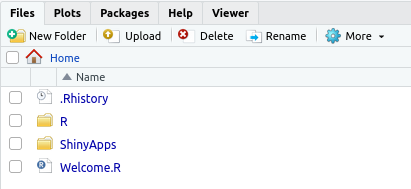
\includegraphics[width=0.5\linewidth]{img/screenshot_rstudio_server_upload} 

}

\caption{File explorer and Upload-button on Rstudio-Server.}\label{fig:ec2rstudioserver}
\end{figure}



To test if all is set up properly to run a in parallel on our EC2 instance, open a new R-script in RStudio-Server and copy/paste the preparatory steps and the simple parallelization example from Section 4.5 into the R-Script.

\begin{Shaded}
\begin{Highlighting}[]
\CommentTok{\# PREPARATION {-}{-}{-}{-}{-}{-}{-}{-}{-}{-}{-}{-}{-}{-}{-}{-}{-}{-}{-}{-}{-}{-}{-}{-}{-}{-}{-}{-}{-}}

\CommentTok{\# packages}
\FunctionTok{library}\NormalTok{(stringr)}

\CommentTok{\# import data}
\NormalTok{marketing }\OtherTok{\textless{}{-}} \FunctionTok{read.csv}\NormalTok{(}\StringTok{"data/marketing\_data.csv"}\NormalTok{)}
\CommentTok{\# clean/prepare data}
\NormalTok{marketing}\SpecialCharTok{$}\NormalTok{Income }\OtherTok{\textless{}{-}} \FunctionTok{as.numeric}\NormalTok{(}\FunctionTok{gsub}\NormalTok{(}\StringTok{"[[:punct:]]"}\NormalTok{, }\StringTok{""}\NormalTok{, marketing}\SpecialCharTok{$}\NormalTok{Income)) }
\NormalTok{marketing}\SpecialCharTok{$}\NormalTok{days\_customer }\OtherTok{\textless{}{-}} \FunctionTok{as.Date}\NormalTok{(}\FunctionTok{Sys.Date}\NormalTok{())}\SpecialCharTok{{-}} \FunctionTok{as.Date}\NormalTok{(marketing}\SpecialCharTok{$}\NormalTok{Dt\_Customer, }\StringTok{"\%m/\%d/\%y"}\NormalTok{)}
\NormalTok{marketing}\SpecialCharTok{$}\NormalTok{Dt\_Customer }\OtherTok{\textless{}{-}} \ConstantTok{NULL}

\CommentTok{\# all sets of independent vars}
\NormalTok{indep }\OtherTok{\textless{}{-}} \FunctionTok{names}\NormalTok{(marketing)[ }\FunctionTok{c}\NormalTok{(}\DecValTok{2}\SpecialCharTok{:}\DecValTok{19}\NormalTok{, }\DecValTok{27}\NormalTok{,}\DecValTok{28}\NormalTok{)]}
\NormalTok{combinations\_list }\OtherTok{\textless{}{-}} \FunctionTok{lapply}\NormalTok{(}\DecValTok{1}\SpecialCharTok{:}\FunctionTok{length}\NormalTok{(indep),}
                            \ControlFlowTok{function}\NormalTok{(x) }\FunctionTok{combn}\NormalTok{(indep, x, }\AttributeTok{simplify =} \ConstantTok{FALSE}\NormalTok{))}
\NormalTok{combinations\_list }\OtherTok{\textless{}{-}} \FunctionTok{unlist}\NormalTok{(combinations\_list, }\AttributeTok{recursive =} \ConstantTok{FALSE}\NormalTok{)}
\NormalTok{models }\OtherTok{\textless{}{-}} \FunctionTok{lapply}\NormalTok{(combinations\_list,}
                 \ControlFlowTok{function}\NormalTok{(x) }\FunctionTok{paste}\NormalTok{(}\StringTok{"Response \textasciitilde{}"}\NormalTok{, }\FunctionTok{paste}\NormalTok{(x, }\AttributeTok{collapse=}\StringTok{"+"}\NormalTok{)))}
\end{Highlighting}
\end{Shaded}

\hypertarget{test-parallelized-code}{%
\paragraph{Test parallelized code}\label{test-parallelized-code}}

Now, we can start testing the code on EC2 without registering the one core for cluster processing. This way \texttt{\%dopart\%} will automatically resort to running the code sequentially. Make sure to set \texttt{N} to 10 (or another small number) for this test.

\begin{Shaded}
\begin{Highlighting}[]
\CommentTok{\# set cores for parallel processing}
\CommentTok{\# ctemp \textless{}{-} makeCluster(ncores)}
\CommentTok{\# registerDoSNOW(ctemp)}

\CommentTok{\# prepare loop}
\NormalTok{N }\OtherTok{\textless{}{-}} \DecValTok{10} \CommentTok{\# just for illustration, the actual code is N \textless{}{-} length(models)}
\CommentTok{\# run loop in parallel}
\NormalTok{pseudo\_Rsq }\OtherTok{\textless{}{-}}
  \FunctionTok{foreach}\NormalTok{ ( }\AttributeTok{i =} \DecValTok{1}\SpecialCharTok{:}\NormalTok{N, }\AttributeTok{.combine =}\NormalTok{ c) }\SpecialCharTok{\%dopar\%}\NormalTok{ \{}
    \CommentTok{\# fit the logit model via maximum likelihood}
\NormalTok{    fit }\OtherTok{\textless{}{-}} \FunctionTok{glm}\NormalTok{(models[[i]], }\AttributeTok{data=}\NormalTok{marketing, }\AttributeTok{family =} \FunctionTok{binomial}\NormalTok{())}
    \CommentTok{\# compute the proportion of deviance explained by the independent vars (\textasciitilde{}R\^{}2)}
    \FunctionTok{return}\NormalTok{(}\DecValTok{1}\SpecialCharTok{{-}}\NormalTok{(fit}\SpecialCharTok{$}\NormalTok{deviance}\SpecialCharTok{/}\NormalTok{fit}\SpecialCharTok{$}\NormalTok{null.deviance))}
\NormalTok{\}}
\end{Highlighting}
\end{Shaded}

Once the test has run through successfully, we are ready to scale up and run the actual workload in parallel in the cloud.

\hypertarget{scale-up-and-run-in-parallel}{%
\subsubsection{Scale up and run in parallel}\label{scale-up-and-run-in-parallel}}

First, switch back to the AWS EC2 console and stop the instance by selecting the tick-mark in the corresponding row, and click on ``Instance state/stop instance''. Once the Instance state is ``Stopped'', click on ``Actions/Instance settings/change instance type''. You will be presented with a drop-down menu from which you can select the new instance type and confirm. The example bellow is based on selecting the \texttt{t2.2xlarge} (with 8 vCPUs and 32MB of RAM). Now you can start the instance again, log in to RStudio-Server (as above) and run the script again but this time with the following lines not commented out (in order to make use of all eight cores).

\begin{Shaded}
\begin{Highlighting}[]
\CommentTok{\# set cores for parallel processing}
\NormalTok{ctemp }\OtherTok{\textless{}{-}} \FunctionTok{makeCluster}\NormalTok{(ncores)}
\FunctionTok{registerDoSNOW}\NormalTok{(ctemp)}
\end{Highlighting}
\end{Shaded}

In order to monitor the usage of computing resources on your instance, switch to the Terminal tab, enter \texttt{htop}, and hit enter. This will open the interactive process viewer called htop. With the default free tier T2.micro instance, you will again notice that only one core is available.

\begin{figure}

{\centering 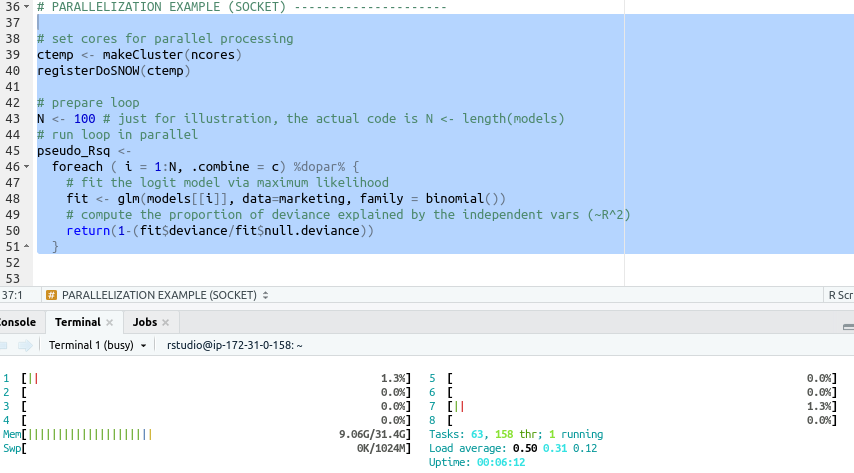
\includegraphics[width=0.8\linewidth]{img/ec2_rstudioserver_htop} 

}

\caption{Monitor resources and proceses with htop.}\label{fig:ec2rstudioserverhtop}
\end{figure}



\hypertarget{scaling-up-with-gpus}{%
\subsection{Scaling up with GPUs}\label{scaling-up-with-gpus}}

To start a ready-made EC2 instance with GPUs and RStudio installed, go to this service provided by RStudio on the AWS Marketplace: \url{https://aws.amazon.com/marketplace/pp/B0785SXYB2}. Click on Subscribe.

\begin{figure}

{\centering 
\includegraphics[width=0.8\linewidth]{img/ec2_gpu1} 

}

\caption{AWS Marketplace product provided by RStudio to run RStudio Server with Tensorflow-GPU on AWS EC2.}\label{fig:ec2gpusetup1}
\end{figure}



Then, click on Continue to Configuration and Continue to Launch. If you want to use the smallest/cheapest EC2 instance, select under ``EC2 Instance Type'' \texttt{g3s.xlarge}. If necessary, create a new key pair under `Key Pair Settings', otherwise keep all the default settings as they are. Then, at the bottom, click on \emph{Launch}. This will launch a new EC2 instance with a GPU and with RStudio server installed.\footnote{Note that you might not have the required vCPU limit to additionally launch such an instance. In that case you will get an error message \texttt{You\ have\ requested\ more\ vCPU\ capacity\ than\ your\ current\ vCPU\ limit\ of\ 0\ allows\ for\ the\ instance\ bucket\ that\ the\ specified\ instance\ type\ belongs\ to.\ Please\ visit\ http://aws.amazon.com/contact-us/ec2-request\ to\ request\ an\ adjustment\ to\ this\ limit.}. Simply follow the indicated URL and send your request to increase the capacity. After your limit is adjusted, click again on Launch as per the procedure outlined above.}

\begin{figure}

{\centering 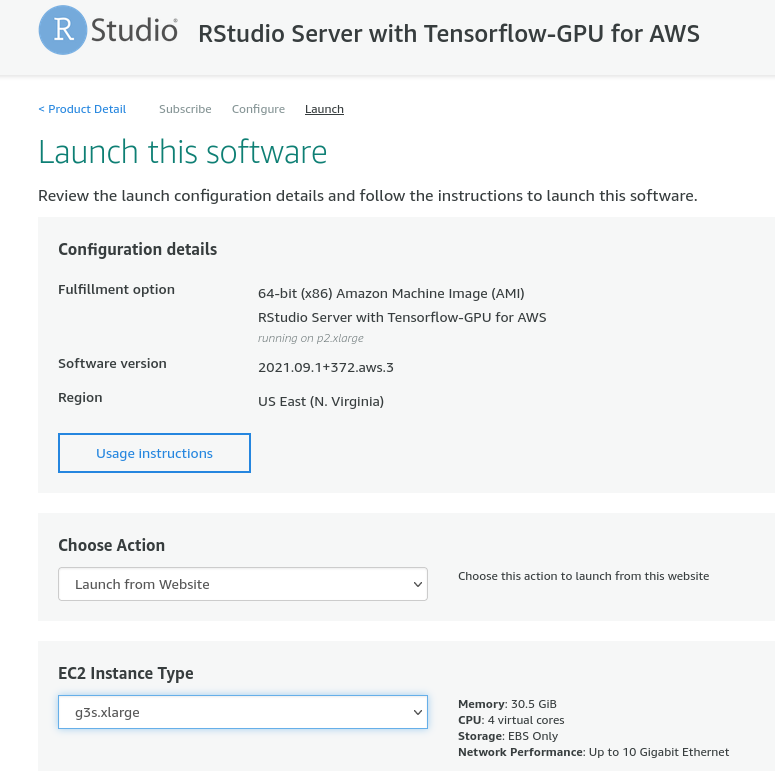
\includegraphics[width=0.6\linewidth]{img/ec2_gpu2} 

}

\caption{Launch RStudio Server with Tensorflow-GPU on AWS EC2.}\label{fig:ec2gpusetup2}
\end{figure}



Once the instance is launched go to the EC2 dashboard, click on the new instance, copy its public dns, open a new browser window and go to \texttt{http://\textless{}ec2\_instance\_public\_dns\textgreater{}:8787}. You should see the RStudio server login. You can log in with username \texttt{rstudio-user} and the instance\_id of your newly created instance as the password.\footnote{It is strongly recommended to change the password afterwards. In o\#rder to do that, click on ``Tools'' and select ``shell''. Then type ``password'' into the shell/terminal and enter the current password (the instance id) and then enter the new password, hit enter, and enter again the new password to confirm.}

\hypertarget{gpus-on-google-colab}{%
\section{GPUs on Google Colab}\label{gpus-on-google-colab}}

Google Colab provides a very easy way to run R code on GPUs from Google Cloud. All you need is a Google account. Open a new browser window, go to \url{https://colab.to/r} and log in with your Google account if prompted to do so. Colab will open a \href{https://en.wikipedia.org/wiki/Project_Jupyter}{Jupyter notebook} with an R runtime. Click on ``Runtime/Change runtime type'' and select in the drop-down menu under `Hardware accelerator' the option `GPU'.

\begin{figure}

{\centering 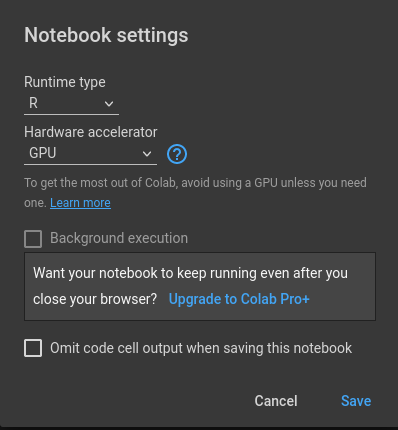
\includegraphics[width=0.5\linewidth]{img/colab_r_gpu} 

}

\caption{Colab notebook with R runtime and GPUs.}\label{fig:colabr}
\end{figure}



Then, you can install the packages you need to work with GPU acceleration (e.g., \texttt{gpuR}, \texttt{keras} and \texttt{tensorflow}) and the code relying on GPU processing will be run on GPUs (or even \href{https://en.wikipedia.org/wiki/Tensor_Processing_Unit}{TPUs}). Under the following link you find a Colab-notebook set up for running a \href{https://tensorflow.rstudio.com/tutorials/beginners/basic-ml/tutorial_basic_classification/}{simply image classification tutorial} with keras on TPUs: \href{https://bit.ly/bda_colab}{bit.ly/bda\_colab}.

\hypertarget{aws-emr-mapreduce-in-the-cloud}{%
\section{AWS EMR: MapReduce in the cloud}\label{aws-emr-mapreduce-in-the-cloud}}

Many cloud computing providers offer specialized services for MapReduce tasks in the cloud. Here we look at a comparatively easy-to-use solution provided by AWS, called Elastic MapReduce (AWS EMR). It allows to set up a Hadoop cluster in the cloud within minutes and requires essentially no additional configuration if the cluster is being used for the kind of data analytics tasks discussed in this book.

Setting up a default AWS EMR cluster via the AWS console is straightforward. Simply go to \texttt{https://console.aws.amazon.com/elasticmapreduce/}, click on ``Create cluster'' and adjust the default selection of settings if necessary. Alternatively, we can set up an EMR cluster via the AWS command-line interface (CLI). In the following tutorials, we will work with AWS EMR via R/Rstudio (specifically, via the package \texttt{sparklyr}). Per default, RStudio is not part of the EMR cluster set up. However, AWS EMR offers a very flexible way to install/configure additional software on virtual EMR clusters via so-called ``bootstrap'' scripts. These scripts can be shared on AWS S3 and used by others, which is what we do in the following cluster set up via the CLI.\footnote{Specifically, we will use the bootstrap script provided by the AWS Big Data Blog, which is stored here: s3://aws-bigdata-blog/artifacts/aws-blog-emr-rstudio-sparklyr/rstudio\_sparklyr\_emr6.sh}

In order to run the cluster set up via AWS CLI shown below, you need an SSH key to later connect to the EMR cluster. If you do not have such an SSH key for AWS yet, follow these instructions to generate one: \url{https://docs.aws.amazon.com/cloudhsm/classic/userguide/generate_ssh_key.html}. In the example below, the key generated in this way is stored in a file called \texttt{sparklyr.pem}.\footnote{If you simply copy-paste the CLI command below to set up an EMR cluster, make sure to name your key file also \texttt{sparklyr.pem}. Otherwise, make sure to change the part in the command referring to the key file accordingly.}

The following command (\texttt{aws\ emr\ create-cluster}) initiates our EMR cluster with a specific set of options (all of these options can also be modified via the AWS console in the browser). \texttt{-\/-applications\ Name=Hadoop\ Name=Spark\ Name=Hive\ Name=Pig\ Name=Tez\ Name=Ganglia} specifies which type of basic applications (that are essential to running different types of MapReduce tasks) should be installed on the cluster. Unless you really know what you are doing, do not change that setting. \texttt{-\/-name\ "EMR\ 6.1\ RStudio\ +\ sparklyr} simply specifies how the newly initiated cluster should be called (this name will then appear on your list of clusters in the AWS console). More relevant for what follows is the line specifying what type of virtual servers (EC2 instances) should be used as part of the cluster: \texttt{-\/-instance-groups\ InstanceGroupType=MASTER,InstanceCount=1,InstanceType=m3.2xlarge} specifies that the one master node (the machine distributing tasks and coordinating the MapReduce procedure) is an instance of type \texttt{m3.2xlarge}; \texttt{InstanceGroupType=CORE,InstanceCount=2,InstanceType=m3.2xlarge} specifies that there are two slave nodes in this cluster, also of type \texttt{m1.medium}.\footnote{Working with one master node of type \texttt{m3.2xlarge} and two slave nodes of the same type only makes sense for test purposes. For an actual} \texttt{-\/-bootstrap-action\ Path=s3://aws-bigdata-blog/artifacts/aws-blog-emr-rstudio-sparklyr/rstudio\_sparklyr\_emr6.sh,Name="Install\ RStudio"} tells the set-up application to run the corresponding bootstrap script on the cluster in order to install the additional software (here RStudio).

Finally, there are two important aspects to note: First, in order to initiate the cluster in this way, you need to have an SSH key pair (for your EC2 instances) set up, which you then instruct the cluster to use with \texttt{KeyName=}. That is, \texttt{KeyName="sparklyr"} means that the user already has create an SSH key pair called \texttt{sparklyr} and that this is the key pair that will be used with the cluster nodes for SSH connections. Second, the \texttt{-\/-region} argument defines in which AWS region the cluster should be created. Importantly, in this particular case, the bootstrap script used to install RStudio on the cluster is stored in the \texttt{us-east-1} region, hence we need to set up the cluster also in this region \texttt{-\/-region\ us-east-1} (otherwise the set up will fail as the set-up application will not find the bootstrap script and terminate with an error!).

\begin{Shaded}
\begin{Highlighting}[]
\ExtensionTok{aws}\NormalTok{ emr create{-}cluster }\DataTypeTok{\textbackslash{}}
\NormalTok{{-}{-}release{-}label emr{-}6.1.0 }\DataTypeTok{\textbackslash{}}
\NormalTok{{-}{-}applications Name=Hadoop Name=Spark Name=Hive Name=Pig Name=Tez Name=Ganglia   }\DataTypeTok{\textbackslash{}}
\NormalTok{{-}{-}name }\StringTok{"EMR 6.1 RStudio + sparklyr"}  \DataTypeTok{\textbackslash{}}
\NormalTok{{-}{-}service{-}role EMR\_DefaultRole }\DataTypeTok{\textbackslash{}}
\NormalTok{{-}{-}instance{-}groups InstanceGroupType=MASTER,InstanceCount=1,InstanceType=m3.2xlarge }\DataTypeTok{\textbackslash{}}
\NormalTok{InstanceGroupType=CORE,InstanceCount=2,InstanceType=m3.2xlarge }\DataTypeTok{\textbackslash{}}
\NormalTok{{-}{-}bootstrap{-}action Path=}\StringTok{\textquotesingle{}s3://aws{-}bigdata{-}blog/artifacts/aws{-}blog{-}emr{-}rstudio{-}sparklyr/rstudio\_sparklyr\_emr6.sh\textquotesingle{}}\NormalTok{,Name=}\StringTok{"Install RStudio"} \AttributeTok{{-}{-}ec2{-}attributes}\NormalTok{ InstanceProfile=EMR\_EC2\_DefaultRole,KeyName=}\StringTok{"sparklyr"} \DataTypeTok{\textbackslash{}}
\NormalTok{{-}{-}configurations }\StringTok{\textquotesingle{}[\{"Classification":"spark","Properties":\{"maximizeResourceAllocation":"true"\}\}]\textquotesingle{}} \DataTypeTok{\textbackslash{}}
\NormalTok{{-}{-}region us{-}east{-}1}
\end{Highlighting}
\end{Shaded}

Setting up this cluster with all the additional software and configurations from the bootstrap script will take around 40 minutes. You can always follow the progress in the AWS console on . Once the cluster is ready, you will see something like this:

\begin{figure}

{\centering 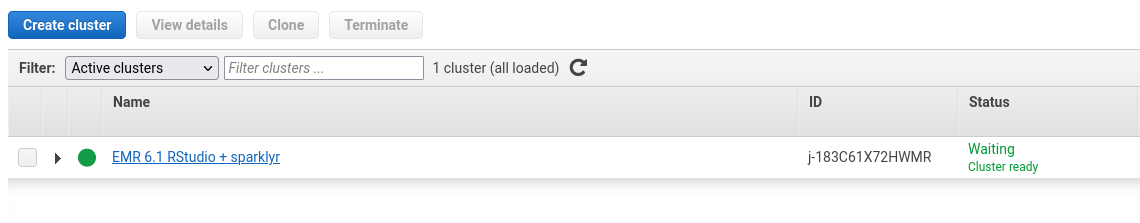
\includegraphics[width=0.8\linewidth]{img/aws_emr_ready} 

}

\caption{AWS EMR console indicating the successful set up of the EMR cluster}\label{fig:emrsetup}
\end{figure}



In order to access RStudio on the EMR cluster's master node via a secure SSH connection, follow these steps:

\begin{itemize}
\item
  First, follow the prerequisites to connect to EMR via SSH: \url{https://docs.aws.amazon.com/emr/latest/ManagementGuide/emr-connect-ssh-prereqs.html}.
\item
  Then initiate the SSH tunnel to the EMR cluster as instructed here: \url{https://docs.aws.amazon.com/emr/latest/ManagementGuide/emr-ssh-tunnel.html}.
\item
  Protect your key-file (\texttt{sparklyr.pem}) by navigating to the location of the key-file on your computer in the terminal and run \texttt{chmod\ 600\ sparklyr.pem} before connecting. Also make sure your IP address is still the one you have entered in the previous step (you can check your current IP address by visiting \url{https://whatismyipaddress.com/}).
\item
  In a browser tab, navigate to the AWS EMR console, click on the newly created cluster and copy the ``Master public DNS''. In the terminal, connect to the EMR cluster via SSH by running \texttt{ssh\ -i\ sparklyr.pem\ -ND\ 8157\ hadoop@master-node-dns} (if you have protected the key-file as super user, i.e.~\texttt{sudo\ chmod}, you will need to use \texttt{sudo\ ssh} here; make sure to replace \texttt{master-node-dns} with the actual dns copied from the AWS EMR console). The terminal will be busy but you won't see any output (if all goes well).
\item
  In your Firefox browser, install the \href{https://addons.mozilla.org/en-US/firefox/addon/foxyproxy-standard/}{FoxyProxy add on}. Follow these instructions to set up the proxy via FoxyProxy: \url{https://docs.aws.amazon.com/emr/latest/ManagementGuide/emr-connect-master-node-proxy.html}.
\item
  Select the newly created Socks5 proxy in FoxyProxy.
\item
  Go to \url{http://localhost:8787/} and enter with username \texttt{hadoop} and password \texttt{hadoop}.
\end{itemize}

Now you can run \texttt{sparklyr} on the AWS EMR cluster. After finishing working with the cluster, make sure to terminate it via the EMR console. This will shot down all the EC2 instances that are part of the cluster (and hence AWS will stop charging you for this).

Once you have connected and logged in to RStudio on the EMR cluster's master node, you can connect the the Rstudio session to the Spark cluster as follows.

\begin{verbatim}
## 
## Attaching package: 'sparklyr'
\end{verbatim}

\begin{verbatim}
## The following object is masked from 'package:stats':
## 
##     filter
\end{verbatim}

\begin{Shaded}
\begin{Highlighting}[]
\CommentTok{\# load packages}
\FunctionTok{library}\NormalTok{(sparklyr)}
\CommentTok{\# connect rstudio session to cluster}
\NormalTok{sc }\OtherTok{\textless{}{-}} \FunctionTok{spark\_connect}\NormalTok{(}\AttributeTok{master =} \StringTok{"yarn"}\NormalTok{)}
\end{Highlighting}
\end{Shaded}

After using the EMR Spark cluster, make sure to terminate the cluster in the AWS EMR console to avoid additional charges. This automatically terminates all the EC2 machines linked to the cluster.

\hypertarget{part-applied-big-data-analytics}{%
\part{Applied Big Data Analytics}\label{part-applied-big-data-analytics}}

Platform: Software and Computing Resources

\hypertarget{forms-of-big-data-and-the-data-pipeline}{%
\chapter{Forms of Big Data and the Data Pipeline}\label{forms-of-big-data-and-the-data-pipeline}}

\hypertarget{unstructured-semi-structured-structured-data}{%
\section{Unstructured, semi-structured, structured data}\label{unstructured-semi-structured-structured-data}}

\hypertarget{data-pipelines-a-systematic-approach-to-processing-big-data}{%
\section{Data pipelines: a systematic approach to processing big data}\label{data-pipelines-a-systematic-approach-to-processing-big-data}}

\begin{center}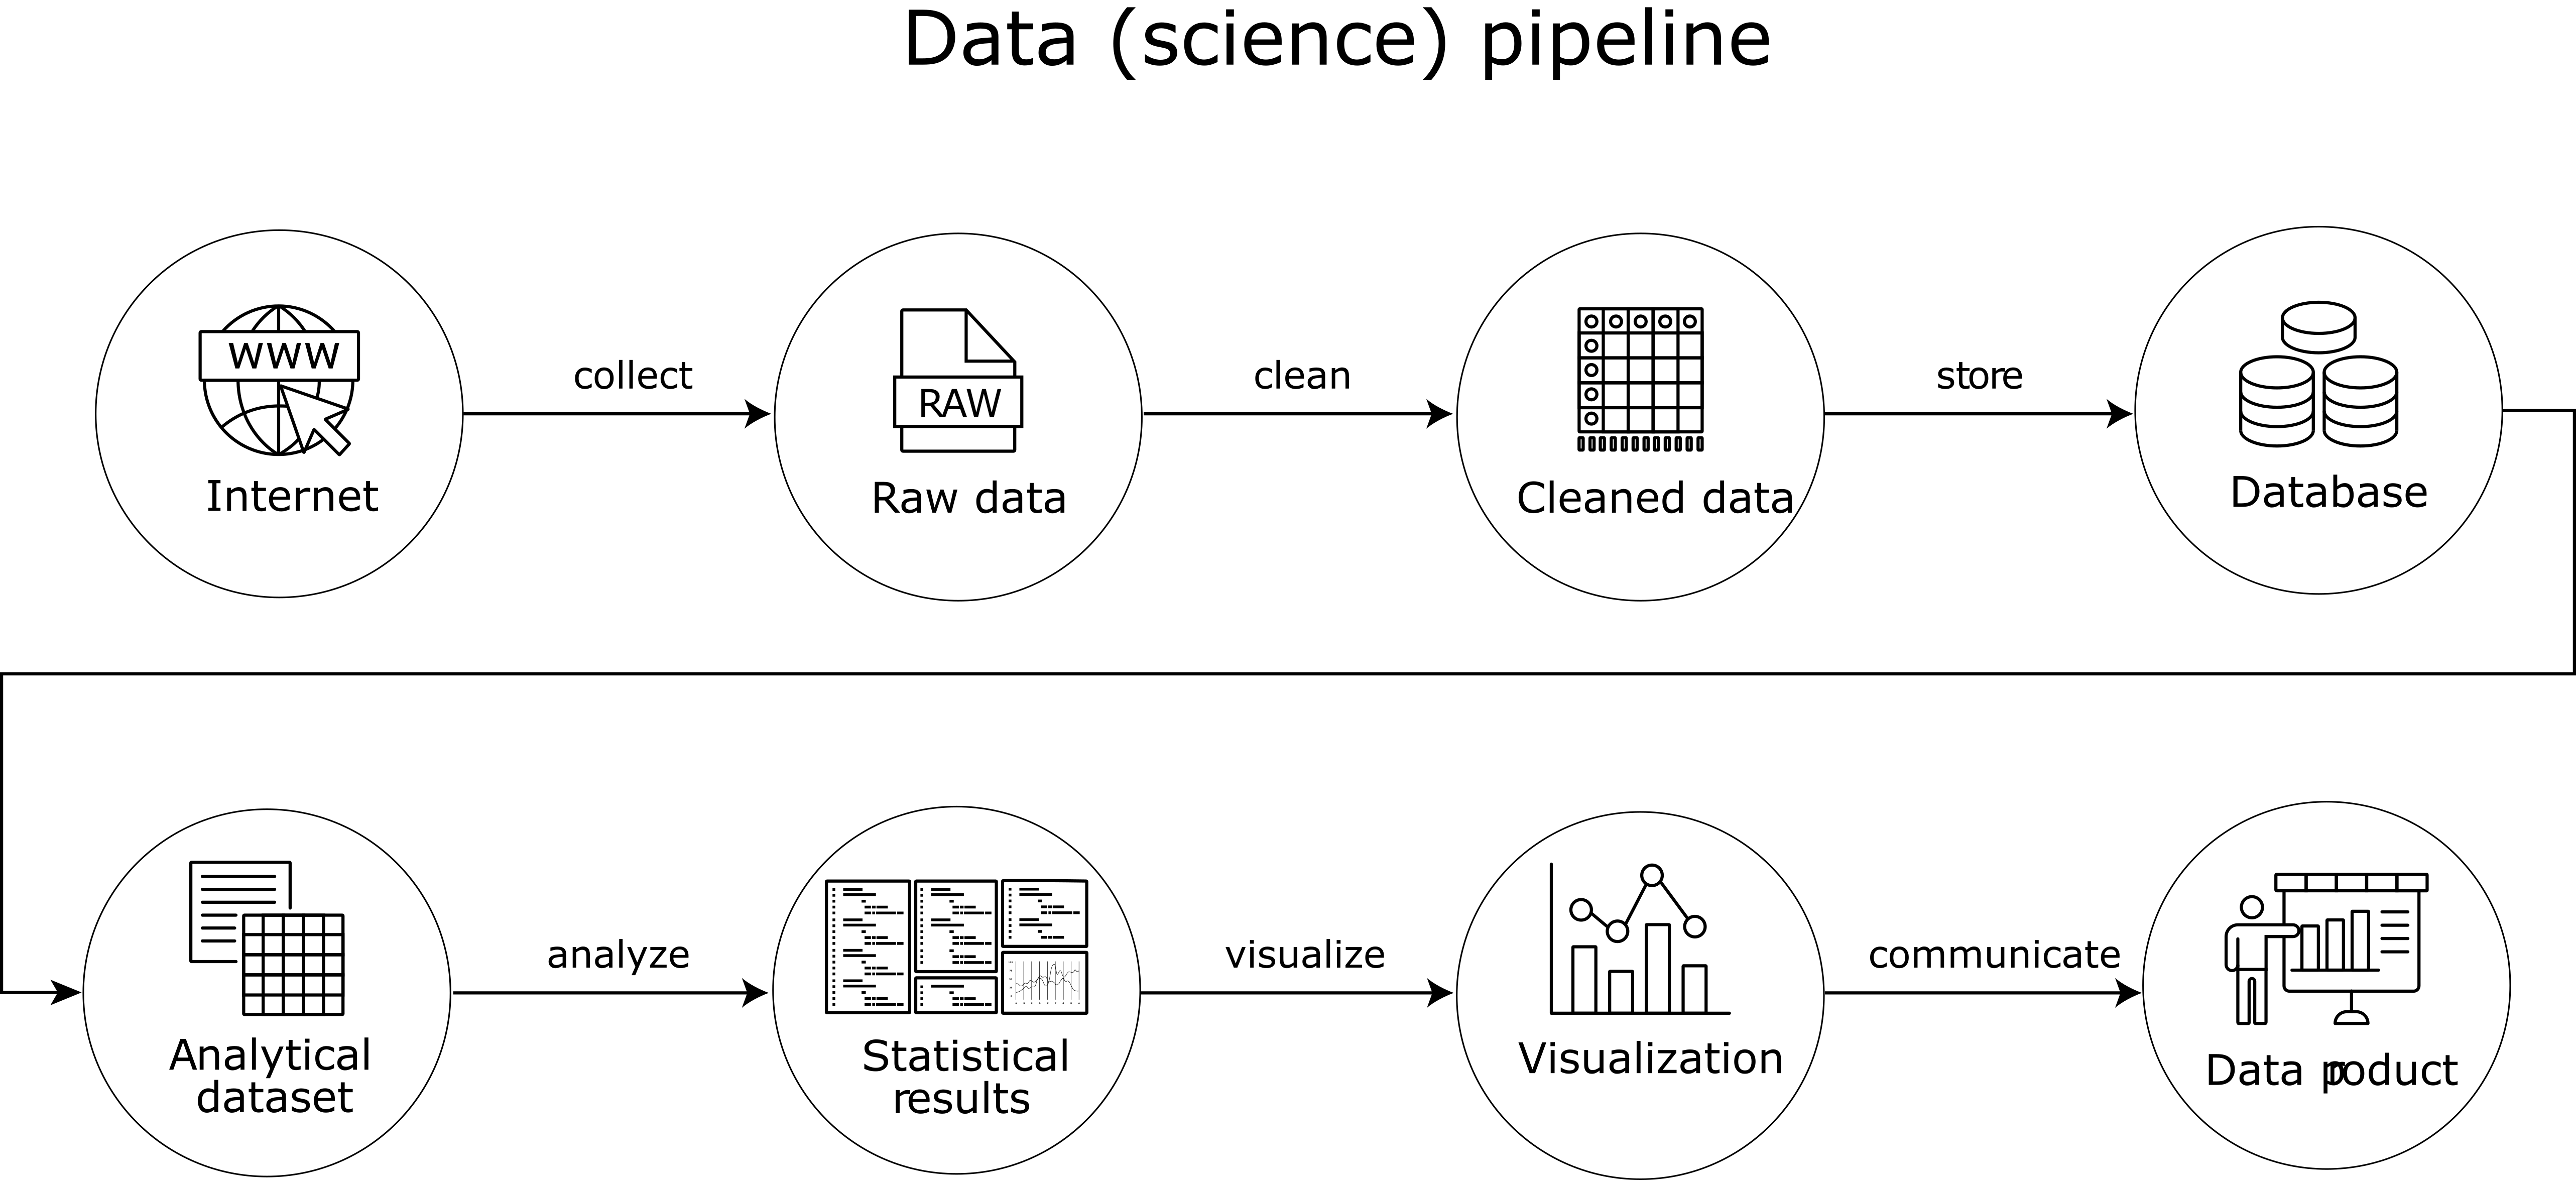
\includegraphics[width=0.8\linewidth]{img/data_pipeline} \end{center}

\hypertarget{data-collection-and-data-storage}{%
\chapter{Data Collection and Data Storage}\label{data-collection-and-data-storage}}

\hypertarget{gathering-and-compilation-of-raw-data}{%
\section{Gathering and compilation of raw data}\label{gathering-and-compilation-of-raw-data}}

\hypertarget{nyc-taxi-data}{%
\subsection{NYC taxi data}\label{nyc-taxi-data}}

The NYC Taxi \& Limousine Commission (TLC) provides detailed data on all trip records including pick-up and drop-off times/locations. When combining all available trip records (2009-2018), we get a rather large data set of over 200GB. The code examples below illustrate how to collect and compile the entire data set. In order to avoid long computing times, the code examples shown below are based on a small sub-set of the actual raw data (however, all examples involving virtual memory, are in theory scalable to the extent of the entire raw data set).

The raw data consists of several monthly CSV-files and can be downloaded via the \href{https://www1.nyc.gov/site/tlc/about/tlc-trip-record-data.page}{TLC's website}. The following short R-script automates the downloading of all available trip-record files. \emph{NOTE}: Downloading all files can take several hours and will occupy over 200GB!

\begin{Shaded}
\begin{Highlighting}[]
\DocumentationTok{\#\#\#\#\#\#\#\#\#\#\#\#\#\#\#\#\#\#\#\#\#\#\#\#\#\#\#\#\#\#\#\#\#}
\CommentTok{\# Fetch all TLC trip recrods}
\CommentTok{\# Data source: }
\CommentTok{\# https://www1.nyc.gov/site/tlc/about/tlc{-}trip{-}record{-}data.page}
\CommentTok{\# Input: Monthly csv files from urls}
\CommentTok{\# Output: one large csv file}
\CommentTok{\# UM, St. Gallen, January 2019}
\DocumentationTok{\#\#\#\#\#\#\#\#\#\#\#\#\#\#\#\#\#\#\#\#\#\#\#\#\#\#\#\#\#\#\#\#\#}

\CommentTok{\# SET UP {-}{-}{-}{-}{-}{-}{-}{-}{-}{-}{-}{-}{-}{-}{-}{-}{-}}

\CommentTok{\# load packages}
\FunctionTok{library}\NormalTok{(data.table)}
\FunctionTok{library}\NormalTok{(rvest)}
\FunctionTok{library}\NormalTok{(httr)}

\CommentTok{\# fix vars}
\NormalTok{BASE\_URL }\OtherTok{\textless{}{-}} \StringTok{"https://s3.amazonaws.com/nyc{-}tlc/trip+data/yellow\_tripdata\_2018{-}01.csv"}
\NormalTok{OUTPUT\_PATH }\OtherTok{\textless{}{-}} \StringTok{"data/tlc\_trips.csv"}
\NormalTok{START\_DATE }\OtherTok{\textless{}{-}} \FunctionTok{as.Date}\NormalTok{(}\StringTok{"2009{-}01{-}01"}\NormalTok{)}
\NormalTok{END\_DATE }\OtherTok{\textless{}{-}} \FunctionTok{as.Date}\NormalTok{(}\StringTok{"2018{-}06{-}01"}\NormalTok{)}


\CommentTok{\# BUILD URLS {-}{-}{-}{-}{-}{-}{-}{-}{-}{-}{-}}

\CommentTok{\# parse base url}
\NormalTok{base\_url }\OtherTok{\textless{}{-}} \FunctionTok{gsub}\NormalTok{(}\StringTok{"2018{-}01.csv"}\NormalTok{, }\StringTok{""}\NormalTok{, BASE\_URL)}
\CommentTok{\# build urls}
\NormalTok{dates }\OtherTok{\textless{}{-}} \FunctionTok{seq}\NormalTok{(}\AttributeTok{from=}\NormalTok{ START\_DATE,}
                   \AttributeTok{to =}\NormalTok{ END\_DATE,}
                   \AttributeTok{by =} \StringTok{"month"}\NormalTok{)}
\NormalTok{year\_months }\OtherTok{\textless{}{-}} \FunctionTok{gsub}\NormalTok{(}\StringTok{"{-}01$"}\NormalTok{, }\StringTok{""}\NormalTok{, }\FunctionTok{as.character}\NormalTok{(dates))}
\NormalTok{data\_urls }\OtherTok{\textless{}{-}} \FunctionTok{paste0}\NormalTok{(base\_url, year\_months, }\StringTok{".csv"}\NormalTok{)}

\CommentTok{\# FETCH AND STACK CSVS {-}{-}{-}{-}{-}{-}{-}{-}{-}{-}{-}{-}{-}{-}{-}{-}}

\CommentTok{\# download, parse all files, write them to one csv}
\ControlFlowTok{for}\NormalTok{ (url }\ControlFlowTok{in}\NormalTok{ data\_urls) \{}
     
     \CommentTok{\# download to temporary file}
\NormalTok{     tmpfile }\OtherTok{\textless{}{-}} \FunctionTok{tempfile}\NormalTok{()}
     \FunctionTok{download.file}\NormalTok{(url, }\AttributeTok{destfile =}\NormalTok{ tmpfile)}
     
     \CommentTok{\# parse downloaded file, write to output csv, remove tempfile}
\NormalTok{     csv\_parsed }\OtherTok{\textless{}{-}} \FunctionTok{fread}\NormalTok{(tmpfile)}
     \FunctionTok{fwrite}\NormalTok{(csv\_parsed,}
            \AttributeTok{file =}\NormalTok{  OUTPUT\_PATH,}
            \AttributeTok{append =} \ConstantTok{TRUE}\NormalTok{)}
     \FunctionTok{unlink}\NormalTok{(tmpfile)}
     
\NormalTok{\}}
\end{Highlighting}
\end{Shaded}

\hypertarget{data-import-and-memory-allocation}{%
\section{Data import and memory allocation}\label{data-import-and-memory-allocation}}

Consider the first steps of a data pipeline in R. The first part of our script to import and clean the data looks as follows.

\begin{Shaded}
\begin{Highlighting}[]
\DocumentationTok{\#\#\#\#\#\#\#\#\#\#\#\#\#\#\#\#\#\#\#\#\#\#\#\#\#\#\#\#\#\#\#\#\#\#\#\#\#\#\#\#\#\#\#\#\#\#\#\#\#\#\#\#\#\#\#\#\#\#\#}
\CommentTok{\# Big Data Statistics: Flights data import and preparation}
\CommentTok{\#}
\CommentTok{\# U. Matter, January 2019}
\DocumentationTok{\#\#\#\#\#\#\#\#\#\#\#\#\#\#\#\#\#\#\#\#\#\#\#\#\#\#\#\#\#\#\#\#\#\#\#\#\#\#\#\#\#\#\#\#\#\#\#\#\#\#\#\#\#\#\#\#\#\#\#}

\CommentTok{\# SET UP {-}{-}{-}{-}{-}{-}{-}{-}{-}{-}{-}{-}{-}{-}{-}{-}{-}}

\CommentTok{\# fix variables}
\NormalTok{DATA\_PATH }\OtherTok{\textless{}{-}} \StringTok{"data/flights.csv"}

\CommentTok{\# DATA IMPORT {-}{-}{-}{-}{-}{-}{-}{-}{-}{-}{-}{-}{-}{-}{-}{-}}
\NormalTok{flights }\OtherTok{\textless{}{-}} \FunctionTok{read.csv}\NormalTok{(DATA\_PATH)}

\CommentTok{\# DATA PREPARATION {-}{-}{-}{-}{-}{-}{-}{-}}
\NormalTok{flights }\OtherTok{\textless{}{-}}\NormalTok{ flights[,}\SpecialCharTok{{-}}\DecValTok{1}\SpecialCharTok{:{-}}\DecValTok{3}\NormalTok{]}
\end{Highlighting}
\end{Shaded}

When running this script, we notice that some of the steps need a noticeable amount of time to process. Moreover, while none of these steps obviously involves a lot of computation (such as a matrix inversion or numerical optimization), it quite likely involves memory allocation. We first read data into RAM (allocated to R by our operating system). It turns out that there are different ways to allocate RAM when reading data from a CSV file. Depending on the amount of data to be read in, one or the other approach might be faster. We first investigate the RAM allocation in R with \texttt{mem\_change()} and \texttt{mem\_used()}.

\begin{Shaded}
\begin{Highlighting}[]
\CommentTok{\# SET UP {-}{-}{-}{-}{-}{-}{-}{-}{-}{-}{-}{-}{-}{-}{-}{-}{-}}

\CommentTok{\# fix variables}
\NormalTok{DATA\_PATH }\OtherTok{\textless{}{-}} \StringTok{"data/flights.csv"}
\CommentTok{\# load packages}
\FunctionTok{library}\NormalTok{(pryr) }


\CommentTok{\# check how much memory is used by R (overall)}
\FunctionTok{mem\_used}\NormalTok{()}
\end{Highlighting}
\end{Shaded}

\begin{verbatim}
## 1.72 GB
\end{verbatim}

\begin{Shaded}
\begin{Highlighting}[]
\CommentTok{\# check the change in memory due to each step}

\CommentTok{\# DATA IMPORT {-}{-}{-}{-}{-}{-}{-}{-}{-}{-}{-}{-}{-}{-}{-}{-}}
\FunctionTok{mem\_change}\NormalTok{(flights }\OtherTok{\textless{}{-}} \FunctionTok{read.csv}\NormalTok{(DATA\_PATH))}
\end{Highlighting}
\end{Shaded}

\begin{verbatim}
## 4.04 MB
\end{verbatim}

\begin{Shaded}
\begin{Highlighting}[]
\CommentTok{\# DATA PREPARATION {-}{-}{-}{-}{-}{-}{-}{-}}
\NormalTok{flights }\OtherTok{\textless{}{-}}\NormalTok{ flights[,}\SpecialCharTok{{-}}\DecValTok{1}\SpecialCharTok{:{-}}\DecValTok{3}\NormalTok{]}

\CommentTok{\# check how much memory is used by R now}
\FunctionTok{mem\_used}\NormalTok{()}
\end{Highlighting}
\end{Shaded}

\begin{verbatim}
## 1.72 GB
\end{verbatim}

The last result is kind of interesting. The object \texttt{flights} must have been larger right after importing it than at the end of the script. We have thrown out several variables, after all. Why does R still use that much memory? R does by default not `clean up' memory unless it is really necessary (meaning no more memory is available). In this case, R has still way more memory available from the operating system, thus there is no need to `collect the garbage' yet. However, we can force R to collect the garbage on the spot with \texttt{gc()}. This can be helpful to better keep track of the memory needed by an analytics script.

\begin{Shaded}
\begin{Highlighting}[]
\FunctionTok{gc}\NormalTok{()}
\end{Highlighting}
\end{Shaded}

\begin{verbatim}
##             used   (Mb) gc trigger   (Mb)  max used
## Ncells   6535541  349.1   10692948  571.1  10692948
## Vcells 169834397 1295.8  409858047 3127.0 284501290
##          (Mb)
## Ncells  571.1
## Vcells 2170.6
\end{verbatim}

Now, let's see how we can improve the performance of this script with regard to memory allocation. Most memory is allocated when importing the file. Obviously, any improvement of the script must still result in importing all the data. However, there are different ways to read data into RAM. \texttt{read.csv()} reads all lines of a csv file consecutively. In contrast, \texttt{data.table::fread()} first `maps' the data file into memory and only then actually reads it in line by line. This involves an additional initial step, but the larger the file, the less relevant is this first step with regard to the total time needed to read all the data into memory. By switching on the \texttt{verbose} option, we can actually see what \texttt{fread} is doing.

\begin{Shaded}
\begin{Highlighting}[]
\CommentTok{\# load packages}
\FunctionTok{library}\NormalTok{(data.table)}
\end{Highlighting}
\end{Shaded}

\begin{verbatim}
## 
## Attaching package: 'data.table'
\end{verbatim}

\begin{verbatim}
## The following object is masked from 'package:pryr':
## 
##     address
\end{verbatim}

\begin{Shaded}
\begin{Highlighting}[]
\CommentTok{\# DATA IMPORT {-}{-}{-}{-}{-}{-}{-}{-}{-}{-}{-}{-}{-}{-}{-}{-}}
\NormalTok{flights }\OtherTok{\textless{}{-}} \FunctionTok{fread}\NormalTok{(DATA\_PATH, }\AttributeTok{verbose =} \ConstantTok{TRUE}\NormalTok{)}
\end{Highlighting}
\end{Shaded}

\begin{verbatim}
##   OpenMP version (_OPENMP)       201511
##   omp_get_num_procs()            12
##   R_DATATABLE_NUM_PROCS_PERCENT  unset (default 50)
##   R_DATATABLE_NUM_THREADS        unset
##   R_DATATABLE_THROTTLE           unset (default 1024)
##   omp_get_thread_limit()         2147483647
##   omp_get_max_threads()          12
##   OMP_THREAD_LIMIT               unset
##   OMP_NUM_THREADS                unset
##   RestoreAfterFork               true
##   data.table is using 6 threads with throttle==1024. See ?setDTthreads.
## Input contains no \n. Taking this to be a filename to open
## [01] Check arguments
##   Using 6 threads (omp_get_max_threads()=12, nth=6)
##   NAstrings = [<<NA>>]
##   None of the NAstrings look like numbers.
##   show progress = 0
##   0/1 column will be read as integer
## [02] Opening the file
##   Opening file data/flights.csv
##   File opened, size = 29.53MB (30960660 bytes).
##   Memory mapped ok
## [03] Detect and skip BOM
## [04] Arrange mmap to be \0 terminated
##   \n has been found in the input and different lines can end with different line endings (e.g. mixed \n and \r\n in one file). This is common and ideal.
## [05] Skipping initial rows if needed
##   Positioned on line 1 starting: <<year,month,day,dep_time,sched_>>
## [06] Detect separator, quoting rule, and ncolumns
##   Detecting sep automatically ...
##   sep=','  with 100 lines of 19 fields using quote rule 0
##   Detected 19 columns on line 1. This line is either column names or first data row. Line starts as: <<year,month,day,dep_time,sched_>>
##   Quote rule picked = 0
##   fill=false and the most number of columns found is 19
## [07] Detect column types, good nrow estimate and whether first row is column names
##   Number of sampling jump points = 100 because (30960659 bytes from row 1 to eof) / (2 * 8882 jump0size) == 1742
##   Type codes (jump 000)    : 555555555C5CCC5555B  Quote rule 0
##   Type codes (jump 100)    : 555555555C5CCC5555B  Quote rule 0
##   'header' determined to be true due to column 1 containing a string on row 1 and a lower type (int32) in the rest of the 10048 sample rows
##   =====
##   Sampled 10048 rows (handled \n inside quoted fields) at 101 jump points
##   Bytes from first data row on line 2 to the end of last row: 30960501
##   Line length: mean=92.03 sd=3.56 min=68 max=98
##   Estimated number of rows: 30960501 / 92.03 = 336403
##   Initial alloc = 370043 rows (336403 + 9%) using bytes/max(mean-2*sd,min) clamped between [1.1*estn, 2.0*estn]
##   =====
## [08] Assign column names
## [09] Apply user overrides on column types
##   After 0 type and 0 drop user overrides : 555555555C5CCC5555B
## [10] Allocate memory for the datatable
##   Allocating 19 column slots (19 - 0 dropped) with 370043 rows
## [11] Read the data
##   jumps=[0..30), chunk_size=1032016, total_size=30960501
## Read 336776 rows x 19 columns from 29.53MB (30960660 bytes) file in 00:00.066 wall clock time
## [12] Finalizing the datatable
##   Type counts:
##         14 : int32     '5'
##          1 : float64   'B'
##          4 : string    'C'
## =============================
##    0.000s (  0%) Memory map 0.029GB file
##    0.003s (  5%) sep=',' ncol=19 and header detection
##    0.000s (  0%) Column type detection using 10048 sample rows
##    0.001s (  1%) Allocation of 370043 rows x 19 cols (0.033GB) of which 336776 ( 91%) rows used
##    0.062s ( 94%) Reading 30 chunks (0 swept) of 0.984MB (each chunk 11225 rows) using 6 threads
##    +    0.018s ( 27%) Parse to row-major thread buffers (grown 0 times)
##    +    0.028s ( 43%) Transpose
##    +    0.016s ( 24%) Waiting
##    0.000s (  0%) Rereading 0 columns due to out-of-sample type exceptions
##    0.066s        Total
\end{verbatim}

Let's put it all together and look at the memory changes and usage. For a fair comparison, we first have to delete \texttt{flights} and collect the garbage with \texttt{gc()}.

\begin{Shaded}
\begin{Highlighting}[]
\CommentTok{\# SET UP {-}{-}{-}{-}{-}{-}{-}{-}{-}{-}{-}{-}{-}{-}{-}{-}{-}}

\CommentTok{\# fix variables}
\NormalTok{DATA\_PATH }\OtherTok{\textless{}{-}} \StringTok{"data/flights.csv"}
\CommentTok{\# load packages}
\FunctionTok{library}\NormalTok{(pryr) }
\FunctionTok{library}\NormalTok{(data.table)}

\CommentTok{\# housekeeping}
\NormalTok{flights }\OtherTok{\textless{}{-}} \ConstantTok{NULL}
\FunctionTok{gc}\NormalTok{()}
\end{Highlighting}
\end{Shaded}

\begin{verbatim}
##             used   (Mb) gc trigger   (Mb)  max used
## Ncells   6593725  352.2   10692948  571.1  10692948
## Vcells 166820133 1272.8  409858047 3127.0 284501290
##          (Mb)
## Ncells  571.1
## Vcells 2170.6
\end{verbatim}

\begin{Shaded}
\begin{Highlighting}[]
\CommentTok{\# check the change in memory due to each step}

\CommentTok{\# DATA IMPORT {-}{-}{-}{-}{-}{-}{-}{-}{-}{-}{-}{-}{-}{-}{-}{-}}
\FunctionTok{mem\_change}\NormalTok{(flights }\OtherTok{\textless{}{-}} \FunctionTok{fread}\NormalTok{(DATA\_PATH))}
\end{Highlighting}
\end{Shaded}

\begin{verbatim}
## 35.8 MB
\end{verbatim}

\hypertarget{efficient-local-data-storage}{%
\section{Efficient local data storage}\label{efficient-local-data-storage}}

In this section, we are concerned with \((I)\) how we can store large data sets permanently on a mass storage device in an efficient way (here, efficient can be understood as `not taking up too much space') and \((II)\) how we can load (parts of) this data set in an efficient way (here, efficient\textasciitilde fast) for analysis.

We look at this problem in two situations:

\begin{itemize}
\tightlist
\item
  The data needs to be stored locally (e.g., on the hard disk of our laptop).
\item
  The data can be stored on a server `in the cloud'.
\end{itemize}

Various tools have been developed over the last few years to improve the efficiency of storing and accessing large amounts of data (see \citet{walkowiak_2016}, chapters 5 and 6 for an overview). Here, we focus on the basic concept of Relational Database Systems (RDBMS) and a well-known tool based on this concept, the Structured Query Language (SQL; more specifically, SQLite)

\hypertarget{rdbms-basics}{%
\subsection{RDBMS basics}\label{rdbms-basics}}

RDBMSs have two key features that tackle the two efficiency concerns mentioned above:

\begin{itemize}
\item
  The \emph{relational data model}: The overall data set is split by columns (covariates) into tables in order to reduce the storage of redundant variable-value repetitions. The resulting database tables are then linked via key-variables (unique identifiers). Thus (simply put), each type of entity on which observations exist resides in its own database table. Within this table, each observation has it's unique id. Keeping the data in such a structure is very efficient in terms of storage space used.
\item
  \emph{Indexing}: The key-columns of the database tables are indexed, meaning (in simple terms) ordered on disk. Indexing a table takes time but it has to be performed only once (unless the content of the table changes). The resulting index is then stored on disk as part of the database. These indices substantially reduce the number of disk accesses required to query/find specific observations. Thus, they make the loading of specific parts of the data for analysis much more efficient.
\end{itemize}

The loading/querying of data from an RDBMS typically involves the selection of specific observations (rows) and covariates (columns) from different tables. Due to the indexing, observations are selected efficiently, and the defined relations between tables (via keys) facilitate the joining of columns to a new table (the queried data).

\hypertarget{efficient-data-access-indices-and-joins-in-sqlite}{%
\subsection{Efficient data access: indices and joins in SQLite}\label{efficient-data-access-indices-and-joins-in-sqlite}}

So far we have only had a look at the very basics of writing SQL code. Let us now further explore SQLite as an easy-to-use and easy-to-set-up relational database solution. In a second step we then look at how to connect to a local SQLite database from within R. First, we switch to the Terminal tab in RStudio, set up a new database called \texttt{air.sqlite}, and import the csv-file \texttt{flights.csv} (used in previous chapters) as a first table.

\begin{Shaded}
\begin{Highlighting}[]
\CommentTok{\# switch to data directory}
\BuiltInTok{cd}\NormalTok{ data}
\CommentTok{\# create database and run sqlite}
\ExtensionTok{sqlite3}\NormalTok{ air.sqlite}
\end{Highlighting}
\end{Shaded}

\begin{Shaded}
\begin{Highlighting}[]
\CommentTok{{-}{-} import csvs}
\NormalTok{.}\KeywordTok{mode}\NormalTok{ csv}
\NormalTok{.import flights.csv flights}
\end{Highlighting}
\end{Shaded}

We check if everything worked out well via the \texttt{.tables} and \texttt{.schema} commands.

\begin{Shaded}
\begin{Highlighting}[]
\NormalTok{.}\KeywordTok{tables}
\NormalTok{.}\KeywordTok{schema}\NormalTok{ flights}
\end{Highlighting}
\end{Shaded}

In \texttt{flights}, each row describes a flight (the day it took place, its origin, its destination etc.). It contains a covariate \texttt{carrier} containing the unique ID of the respective airline/carrier carrying out the flight as well as the covariates \texttt{origin} and \texttt{dest}. The latter two variables contain the unique IATA-codes of the airports from which the flights departed and where they arrived, respectively. In \texttt{flights} we thus have observations at the level of individual flights.

Now we extend our database in a meaningful way, following the relational data model idea. First we download two additional csv files containing data that relate to the flights table:

\begin{itemize}
\tightlist
\item
  \href{http://stat-computing.org/dataexpo/2009/airports.csv}{\texttt{airports.csv}}: Describes the locations of US Airports (relates to \texttt{origin} and \texttt{dest}).
\item
  \href{http://stat-computing.org/dataexpo/2009/carriers.csv}{\texttt{carriers.csv}}: A listing of carrier codes with full names (relates to the \texttt{carrier}-column in \texttt{flights}.
\end{itemize}

In this code example, the two csvs have already been downloaded to the \texttt{materials/data}-folder.

\begin{Shaded}
\begin{Highlighting}[]
\CommentTok{{-}{-} import airport data}
\NormalTok{.}\KeywordTok{mode}\NormalTok{ csv}
\NormalTok{.import airports.csv airports}
\NormalTok{.import carriers.csv carriers}

\CommentTok{{-}{-} inspect the result}
\NormalTok{.}\KeywordTok{tables}
\NormalTok{.}\KeywordTok{schema}\NormalTok{ airports}
\NormalTok{.}\KeywordTok{schema}\NormalTok{ carriers}
\end{Highlighting}
\end{Shaded}

Now we can run our first query involving the relation between tables. The aim of the exercise is to query flights data (information on departure delays per flight number and date; from the \texttt{flights}-table) for all \texttt{United\ Air\ Lines\ Inc.}-flights (information from the \texttt{carriers} table ) departing from \texttt{Newark\ Intl} airport (information from the \texttt{airports}-table). In addition, we want the resulting table ordered by flight number. For the sake of the exercise, we only show the first 10 results of this query (\texttt{LIMIT\ 10}).

\begin{Shaded}
\begin{Highlighting}[]
\KeywordTok{SELECT} 
\DataTypeTok{year}\NormalTok{,}
\DataTypeTok{month}\NormalTok{, }
\DataTypeTok{day}\NormalTok{,}
\NormalTok{dep\_delay,}
\NormalTok{flight}
\KeywordTok{FROM}\NormalTok{ (flights }\KeywordTok{INNER} \KeywordTok{JOIN}\NormalTok{ airports }\KeywordTok{ON}\NormalTok{ flights.origin}\OperatorTok{=}\NormalTok{airports.iata) }
\KeywordTok{INNER} \KeywordTok{JOIN}\NormalTok{ carriers }\KeywordTok{ON}\NormalTok{ flights.carrier }\OperatorTok{=}\NormalTok{ carriers.Code}
\KeywordTok{WHERE}\NormalTok{ carriers.Description }\OperatorTok{=} \StringTok{\textquotesingle{}United Air Lines Inc.\textquotesingle{}}
\KeywordTok{AND}\NormalTok{ airports.airport }\OperatorTok{=} \StringTok{\textquotesingle{}Newark Intl\textquotesingle{}}
\KeywordTok{ORDER} \KeywordTok{BY}\NormalTok{ flight}
\KeywordTok{LIMIT} \DecValTok{10}\NormalTok{;}
\end{Highlighting}
\end{Shaded}

\begin{table}

\caption{\label{tab:unnamed-chunk-126}Displaying records 1 - 10}
\centering
\begin{tabular}[t]{r|r|r|r|r}
\hline
year & month & day & dep\_delay & flight\\
\hline
2013 & 1 & 4 & 0 & 1\\
\hline
2013 & 1 & 5 & -2 & 1\\
\hline
2013 & 3 & 6 & 1 & 1\\
\hline
2013 & 2 & 13 & -2 & 3\\
\hline
2013 & 2 & 16 & -9 & 3\\
\hline
2013 & 2 & 20 & 3 & 3\\
\hline
2013 & 2 & 23 & -5 & 3\\
\hline
2013 & 2 & 26 & 24 & 3\\
\hline
2013 & 2 & 27 & 10 & 3\\
\hline
2013 & 1 & 5 & 3 & 10\\
\hline
\end{tabular}
\end{table}

Note that this query has been executed without indexing any of the tables first. Thus SQLite could not take any `shortcuts' when matching the ID columns in order to join the tables for the query output. That is, SQLite had to scan the entire columns to find the matches. Now we index the respective id columns and re-run the query.

\begin{Shaded}
\begin{Highlighting}[]
\KeywordTok{CREATE} \KeywordTok{INDEX}\NormalTok{ iata\_airports }\KeywordTok{ON}\NormalTok{ airports (iata);}
\KeywordTok{CREATE} \KeywordTok{INDEX}\NormalTok{ origin\_flights }\KeywordTok{ON}\NormalTok{ flights (origin);}
\KeywordTok{CREATE} \KeywordTok{INDEX}\NormalTok{ carrier\_flights }\KeywordTok{ON}\NormalTok{ flights (carrier);}
\KeywordTok{CREATE} \KeywordTok{INDEX}\NormalTok{ code\_carriers }\KeywordTok{ON}\NormalTok{ carriers (code);}
\end{Highlighting}
\end{Shaded}

Note that SQLite optimizes the efficiency of the query without our explicit instructions. If there are indices it can use to speed up the query, it will do so.

\begin{Shaded}
\begin{Highlighting}[]
\KeywordTok{SELECT} 
\DataTypeTok{year}\NormalTok{,}
\DataTypeTok{month}\NormalTok{, }
\DataTypeTok{day}\NormalTok{,}
\NormalTok{dep\_delay,}
\NormalTok{flight}
\KeywordTok{FROM}\NormalTok{ (flights }\KeywordTok{INNER} \KeywordTok{JOIN}\NormalTok{ airports }\KeywordTok{ON}\NormalTok{ flights.origin}\OperatorTok{=}\NormalTok{airports.iata) }
\KeywordTok{INNER} \KeywordTok{JOIN}\NormalTok{ carriers }\KeywordTok{ON}\NormalTok{ flights.carrier }\OperatorTok{=}\NormalTok{ carriers.Code}
\KeywordTok{WHERE}\NormalTok{ carriers.Description }\OperatorTok{=} \StringTok{\textquotesingle{}United Air Lines Inc.\textquotesingle{}}
\KeywordTok{AND}\NormalTok{ airports.airport }\OperatorTok{=} \StringTok{\textquotesingle{}Newark Intl\textquotesingle{}}
\KeywordTok{ORDER} \KeywordTok{BY}\NormalTok{ flight}
\KeywordTok{LIMIT} \DecValTok{10}\NormalTok{;}
\end{Highlighting}
\end{Shaded}

\begin{table}

\caption{\label{tab:unnamed-chunk-128}Displaying records 1 - 10}
\centering
\begin{tabular}[t]{r|r|r|r|r}
\hline
year & month & day & dep\_delay & flight\\
\hline
2013 & 1 & 4 & 0 & 1\\
\hline
2013 & 1 & 5 & -2 & 1\\
\hline
2013 & 3 & 6 & 1 & 1\\
\hline
2013 & 2 & 13 & -2 & 3\\
\hline
2013 & 2 & 16 & -9 & 3\\
\hline
2013 & 2 & 20 & 3 & 3\\
\hline
2013 & 2 & 23 & -5 & 3\\
\hline
2013 & 2 & 26 & 24 & 3\\
\hline
2013 & 2 & 27 & 10 & 3\\
\hline
2013 & 1 & 5 & 3 & 10\\
\hline
\end{tabular}
\end{table}

You find the final \texttt{air.sqlite}, including all the indices and tables as \texttt{materials/data/air\_final.sqlite} in the course's code repository.

\hypertarget{connecting-r-to-rdbms}{%
\section{Connecting R to RDBMS}\label{connecting-r-to-rdbms}}

The R-package \texttt{RSQLite} embeds SQLite in R. That is, it provides functions that allow us to use SQLite directly from within R. You will see that the combinaiton of SQLite with R is a simple but very practical approach to work with very efficiently (and locally) stored data sets. In the following example, we explore how \texttt{RSQLite} can be used to set up and query the \texttt{air.sqlite} shown in the example above.

\hypertarget{creating-a-new-database-with-rsqlite}{%
\subsection{\texorpdfstring{Creating a new database with \texttt{RSQLite}}{Creating a new database with RSQLite}}\label{creating-a-new-database-with-rsqlite}}

Similarly to the raw SQLite-syntax, connecting to a database that does not exist yet, actually creates this (empty database). Note that for all interactions with the database from within R, we need to refer to the connection (here: \texttt{con\_air}).

\begin{Shaded}
\begin{Highlighting}[]
\CommentTok{\# load packages}
\FunctionTok{library}\NormalTok{(RSQLite)}

\CommentTok{\# initiate the database}
\NormalTok{con\_air }\OtherTok{\textless{}{-}} \FunctionTok{dbConnect}\NormalTok{(}\FunctionTok{SQLite}\NormalTok{(), }\StringTok{"data/air.sqlite"}\NormalTok{)}
\end{Highlighting}
\end{Shaded}

\hypertarget{importing-data}{%
\subsection{Importing data}\label{importing-data}}

With \texttt{RSQLite} we can easily add \texttt{data.frame}s as SQLite tables to the database.

\begin{Shaded}
\begin{Highlighting}[]
\CommentTok{\# import data into current R sesssion}
\NormalTok{flights }\OtherTok{\textless{}{-}} \FunctionTok{fread}\NormalTok{(}\StringTok{"data/flights.csv"}\NormalTok{)}
\NormalTok{airports }\OtherTok{\textless{}{-}} \FunctionTok{fread}\NormalTok{(}\StringTok{"data/airports.csv"}\NormalTok{)}
\NormalTok{carriers }\OtherTok{\textless{}{-}} \FunctionTok{fread}\NormalTok{(}\StringTok{"data/carriers.csv"}\NormalTok{)}

\CommentTok{\# add tables to database}
\FunctionTok{dbWriteTable}\NormalTok{(con\_air, }\StringTok{"flights"}\NormalTok{, flights)}
\FunctionTok{dbWriteTable}\NormalTok{(con\_air, }\StringTok{"airports"}\NormalTok{, airports)}
\FunctionTok{dbWriteTable}\NormalTok{(con\_air, }\StringTok{"carriers"}\NormalTok{, carriers)}
\end{Highlighting}
\end{Shaded}

\hypertarget{issue-queries}{%
\subsection{Issue queries}\label{issue-queries}}

Now we can query the database from within R. By default, \texttt{RSQLite} returns the query results as \texttt{data.frame}s. Queries are simply character strings written in SQLite.

\begin{Shaded}
\begin{Highlighting}[]
\CommentTok{\# define query}
\NormalTok{delay\_query }\OtherTok{\textless{}{-}}
\StringTok{"SELECT }
\StringTok{year,}
\StringTok{month, }
\StringTok{day,}
\StringTok{dep\_delay,}
\StringTok{flight}
\StringTok{FROM (flights INNER JOIN airports ON flights.origin=airports.iata) }
\StringTok{INNER JOIN carriers ON flights.carrier = carriers.Code}
\StringTok{WHERE carriers.Description = \textquotesingle{}United Air Lines Inc.\textquotesingle{}}
\StringTok{AND airports.airport = \textquotesingle{}Newark Intl\textquotesingle{}}
\StringTok{ORDER BY flight}
\StringTok{LIMIT 10;}
\StringTok{"}

\CommentTok{\# issue query}
\NormalTok{delays\_df }\OtherTok{\textless{}{-}} \FunctionTok{dbGetQuery}\NormalTok{(con\_air, delay\_query)}
\NormalTok{delays\_df}
\end{Highlighting}
\end{Shaded}

When done working with the database, we close the connection to the database with \texttt{dbDisconnect(con)}.

\hypertarget{cloud-solutions-for-big-data-storage}{%
\section{Cloud solutions for (big) data storage}\label{cloud-solutions-for-big-data-storage}}

As outlined in the previous section, RDBMSs are a very practical tool to store the structured data of an analytics project locally in a database. A local SQLite database can easily be set up and accessed via R, allowing to write the whole data pipeline from data gathering to filtering, aggregating and finally analyzing in R. In contrast to directly working with CSV files, using SQLite has the advantage of organizing the data access much more efficiently in terms of RAM. Only the final result of a query is really loaded fully into R's memory.

If mass storage space is too sparse or if RAM is nevertheless not sufficient, even when organizing data access via SQLite, several cloud solutions come to the rescue. Although you could also rent a traditional web server and host a SQL database there, this is usually not worth the while for a data analytics project. In the next section we thus look at three important cases of how to store data as part of an analytics project: \emph{RDBMS in the cloud}, a serverless \emph{data warehouse} solution for large datasets called \emph{Google BigQuery}, and a simple storage service to use as a \emph{data lake} called \emph{AWS S3}. All of these solutions are discussed from a data analytics perspective, and for all of these solutions we will look at how to make use of them from within R.

\hypertarget{easy-to-use-rdbms-in-the-cloud-aws-rds}{%
\subsection{Easy-to-use RDBMS in the cloud: AWS RDS}\label{easy-to-use-rdbms-in-the-cloud-aws-rds}}

Once we have set up RStudio Server on an EC2 instance, we can run the SQLite examples shown above on it. There are no additional steps needed to install SQLite. However, when using RDBMSs in the cloud, we typically have a more sophisticated implementation than SQLite in mind. Particularly, we want to set up an actual RDBMS-server running in the cloud to which several clients can connect (e.g., via RStudio Server).

AWS' Relational Database Service (RDS) provides an easy way to set up and run a SQL database in the cloud. The great advantage for users new to RDBMS/SQL is that you do not have to manually set up a server (e.g.~a EC2 instance) and install/configure the SQL server. Instead you can directly set up a fully functioning relational database in the cloud.

In a first step, open the AWS console and search for/select ``RDS'' in the search bar. Then, click on ``Create database'' in the lower part of the landing page.

\begin{figure}

{\centering 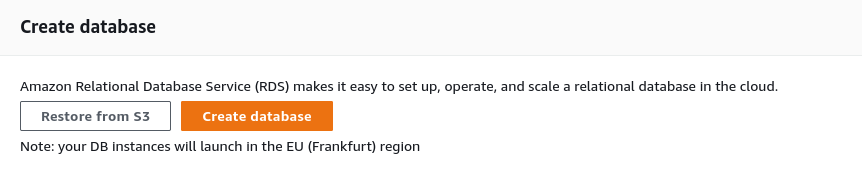
\includegraphics[width=0.8\linewidth]{img/aws_rds_create} 

}

\caption{Create a managed relational database on AWS RDS.}\label{fig:rdscreate}
\end{figure}



On the next page, select ``Easy create'', ``MySQL'', and the ``Free tier'' DB instance size. Further down you will have to set the database instance identifier the user name and a password.

\begin{figure}

{\centering 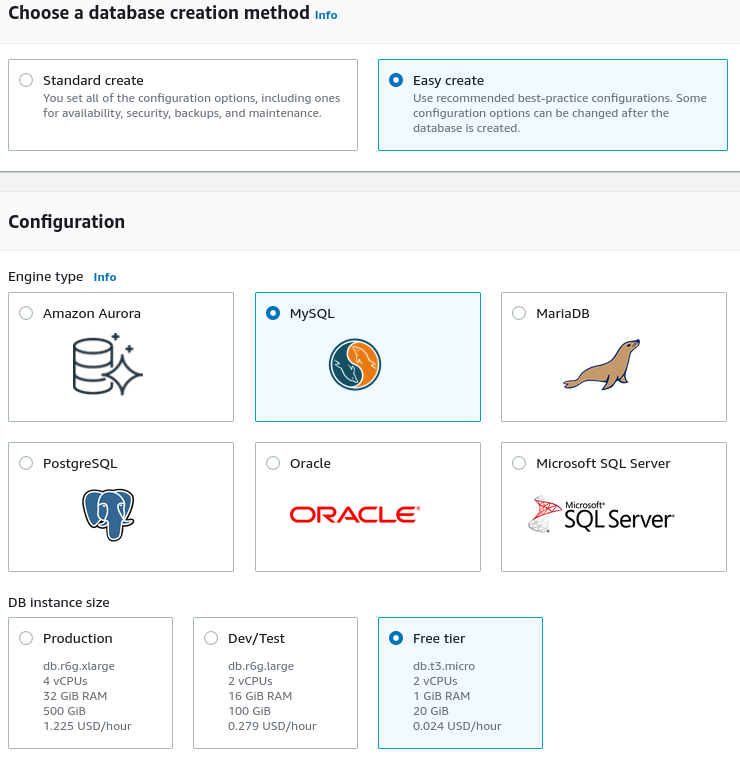
\includegraphics[width=0.8\linewidth]{img/aws_rds_easycreate} 

}

\caption{Easy creation of a RDS MySQL DB.}\label{fig:rdseasy}
\end{figure}



Once the database instance is ready, you will see it in the databases overview. Click on the DB identifier (the name of your database shown in the list of databases) and click on modify (button in the upper-right corner). In the ``Connectivity'' panel under ``Additional configuration'', select \emph{Publicly accessible} (this is necessary to interact with the DB from your local machine), and save the settings. Back on the overview page of your database, under ``Connectivity \& security'', click on the link under the VPC security groups, scroll down and select the ``Inbound rules'' tab. Edit the inbound rule to allow any IP4 inbound traffic.\footnote{Note that this is not generally recommendable. Only do this to get familiar with the service and to test some code.}

\begin{figure}

{\centering 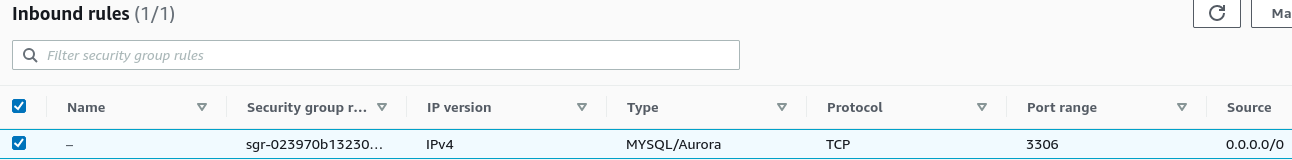
\includegraphics[width=0.8\linewidth]{img/rds_inboundrules} 

}

\caption{Allow all IP4 inbound traffic (set Source to \texttt{0.0.0.0/0}).}\label{fig:rdsinboundrules}
\end{figure}



Now we can connect to the instance via the \texttt{RMySQL} package. Before loading data, we first have to initiate a new database (in contrast, this is done automatically when connecting to a SQLite database).

\begin{Shaded}
\begin{Highlighting}[]
\CommentTok{\# load packages}
\FunctionTok{library}\NormalTok{(RMySQL)}
\FunctionTok{library}\NormalTok{(data.table)}

\CommentTok{\# fix vars}
\NormalTok{RDS\_ENDPOINT }\OtherTok{\textless{}{-}} \StringTok{"MY{-}ENDPOINT"} \CommentTok{\# replace this with the Endpoint shown in the AWS RDS console}
\NormalTok{PW }\OtherTok{\textless{}{-}} \StringTok{"MY{-}PW"} \CommentTok{\# replace this with the password you have set when initiating the RDS DB on AWS}

\CommentTok{\# connect to DB}
\NormalTok{con\_rds }\OtherTok{\textless{}{-}} \FunctionTok{dbConnect}\NormalTok{(RMySQL}\SpecialCharTok{::}\FunctionTok{MySQL}\NormalTok{(),}
                 \AttributeTok{host=}\NormalTok{RDS\_ENDPOINT,}
                 \AttributeTok{port=}\DecValTok{3306}\NormalTok{,}
                 \AttributeTok{username=}\StringTok{"admin"}\NormalTok{,}
                 \AttributeTok{password=}\NormalTok{PW)}

\CommentTok{\# initiate a new database on the MySQL RDS instance}
\FunctionTok{dbSendQuery}\NormalTok{(con\_rds, }\StringTok{"CREATE DATABASE air"}\NormalTok{)}

\CommentTok{\# disconnect and re{-}connect directly to the new DB}
\FunctionTok{dbDisconnect}\NormalTok{(con\_rds)}
\NormalTok{con\_rds }\OtherTok{\textless{}{-}} \FunctionTok{dbConnect}\NormalTok{(RMySQL}\SpecialCharTok{::}\FunctionTok{MySQL}\NormalTok{(),}
                 \AttributeTok{host=}\NormalTok{RDS\_ENDPOINT,}
                 \AttributeTok{port=}\DecValTok{3306}\NormalTok{,}
                 \AttributeTok{username=}\StringTok{"admin"}\NormalTok{,}
                 \AttributeTok{dbname=}\StringTok{"air"}\NormalTok{,}
                 \AttributeTok{password=}\NormalTok{PW)}
\end{Highlighting}
\end{Shaded}

\texttt{RMySQL} and \texttt{RSQLite} are both building on the \texttt{DBI} package, which generalizes how we can interact with SQL-type databases via R. This makes it straightforward to apply what we have learned so far by interacting with our local SQLite database to interactions with other databases. As soon as the connection to the new database is established, we can essentially use the same R functions as above to create new tables and import data.

\begin{Shaded}
\begin{Highlighting}[]
\CommentTok{\# import data into current R sesssion}
\NormalTok{flights }\OtherTok{\textless{}{-}} \FunctionTok{fread}\NormalTok{(}\StringTok{"data/flights.csv"}\NormalTok{)}
\NormalTok{airports }\OtherTok{\textless{}{-}} \FunctionTok{fread}\NormalTok{(}\StringTok{"data/airports.csv"}\NormalTok{)}
\NormalTok{carriers }\OtherTok{\textless{}{-}} \FunctionTok{fread}\NormalTok{(}\StringTok{"data/carriers.csv"}\NormalTok{)}

\CommentTok{\# add tables to database}
\FunctionTok{dbWriteTable}\NormalTok{(con\_rds, }\StringTok{"flights"}\NormalTok{, flights)}
\FunctionTok{dbWriteTable}\NormalTok{(con\_rds, }\StringTok{"airports"}\NormalTok{, airports)}
\FunctionTok{dbWriteTable}\NormalTok{(con\_rds, }\StringTok{"carriers"}\NormalTok{, carriers)}
\end{Highlighting}
\end{Shaded}

Finally, we can query our RDS MySQL database on AWS.

\begin{Shaded}
\begin{Highlighting}[]
\CommentTok{\# define query}
\NormalTok{delay\_query }\OtherTok{\textless{}{-}}
\StringTok{"SELECT }
\StringTok{year,}
\StringTok{month, }
\StringTok{day,}
\StringTok{dep\_delay,}
\StringTok{flight}
\StringTok{FROM (flights INNER JOIN airports ON flights.origin=airports.iata) }
\StringTok{INNER JOIN carriers ON flights.carrier = carriers.Code}
\StringTok{WHERE carriers.Description = \textquotesingle{}United Air Lines Inc.\textquotesingle{}}
\StringTok{AND airports.airport = \textquotesingle{}Newark Intl\textquotesingle{}}
\StringTok{ORDER BY flight}
\StringTok{LIMIT 10;}
\StringTok{"}

\CommentTok{\# issue query}
\NormalTok{delays\_df }\OtherTok{\textless{}{-}} \FunctionTok{dbGetQuery}\NormalTok{(con\_rds, delay\_query)}
\NormalTok{delays\_df}
\end{Highlighting}
\end{Shaded}

\hypertarget{database-server-in-the-cloud-mariadb-on-an-ec2-instance}{%
\subsection{Database server in the cloud: MariaDB on an EC2 instance}\label{database-server-in-the-cloud-mariadb-on-an-ec2-instance}}

Working with an SQL database in the cloud via AWS RDS is probably sufficient for most simple use cases. However, for some projects you might want to have more flexibility regarding settings and configurations. A practical solution to this is to set up ``manually'' a SQL-server on an EC2 instance (and then work with it via RStudio-Server). The following example, based on \citet{walkowiak_2016}, guides you through the first step to set up such a database in the cloud. For most of the installation steps you are referred to the respective pages in \citet{walkowiak_2016} (Chapter 5: 'MariaDB with R on a Amazon EC2 instance, pages 255ff). However, since some of the steps shown in the book are outdated, the example below hints to some alternative/additional steps needed to make the database run on an Ubuntu 18.04 machine.

After launching the EC2 instance on AWS, use the following terminal commands to install R:

\begin{Shaded}
\begin{Highlighting}[]
\CommentTok{\# update ubuntu packages}
 \FunctionTok{sudo}\NormalTok{ apt{-}get update}
 \FunctionTok{sudo}\NormalTok{ apt{-}get upgrade}
\end{Highlighting}
\end{Shaded}

\begin{Shaded}
\begin{Highlighting}[]
\FunctionTok{sudo}\NormalTok{ apt{-}get install r{-}base}
\end{Highlighting}
\end{Shaded}

and to install RStudio Server (on Ubuntu 18.04, as of April 2020):

\begin{Shaded}
\begin{Highlighting}[]
\FunctionTok{sudo}\NormalTok{ apt{-}get install gdebi{-}core}
\FunctionTok{wget}\NormalTok{ https://download2.rstudio.org/server/bionic/amd64/rstudio{-}server{-}1.2.5033{-}amd64.deb}
\FunctionTok{sudo}\NormalTok{ gdebi rstudio{-}server{-}1.2.5033{-}amd64.deb}
\end{Highlighting}
\end{Shaded}

Following \citet{walkowiak_2016} (pages 257f), we first set up a new user and give it permissions to \texttt{ssh} directly to the EC2 instance (this way we can then more easily upload data `for this user').

\begin{Shaded}
\begin{Highlighting}[]
\CommentTok{\# create user}
\FunctionTok{sudo}\NormalTok{ adduser umatter }
\end{Highlighting}
\end{Shaded}

When prompted for additional information just hit enter (for default). Now we can grant the user the permissions

\begin{Shaded}
\begin{Highlighting}[]
\FunctionTok{sudo}\NormalTok{ cp }\AttributeTok{{-}r}\NormalTok{ /home/ubuntu/.ssh /home/umatter/}
\BuiltInTok{cd}\NormalTok{ /home/umatter/}
\FunctionTok{sudo}\NormalTok{ chown }\AttributeTok{{-}R}\NormalTok{ umatter:umatter .ssh}
\end{Highlighting}
\end{Shaded}

Then install MariaDB as follows.

\begin{Shaded}
\begin{Highlighting}[]
\FunctionTok{sudo}\NormalTok{ apt update}
\FunctionTok{sudo}\NormalTok{ apt install mariadb{-}server}
\FunctionTok{sudo}\NormalTok{ apt install libmariadbclient{-}dev}
\FunctionTok{sudo}\NormalTok{ apt install libxml2{-}dev }\CommentTok{\# needed later (dependency for some R packages)}
\end{Highlighting}
\end{Shaded}

If prompted to set a password for the root database user (user with all database priviledges), type in and confirm the chosen password.\footnote{Below it is shown how to do this `manually', if not promted at this step.}

\hypertarget{data-import}{%
\subsubsection{Data import}\label{data-import}}

With the permissions set above, we can send data from the local machine directly to the instance via \texttt{ssh}. We use this to first transfer the raw data to the instance and then import it to the database.

The aim is to import the same simple data set \texttt{economics.csv} used in the local SQLite examples of Lecture 7. Following the instructions of \citet{walkowiak_2016}, pages 252 to 254, we upload the \texttt{economics.csv} file (instead of the example data used in \citet{walkowiak_2016}). Note that in all the code examples below, the username is \texttt{umatter}, and the IP-address will have to be replaced with the public IP-address of your EC2 instance.

Open a new terminal window and send the \texttt{economics.csv} data as follows to the instance.

\begin{Shaded}
\begin{Highlighting}[]
\CommentTok{\# from the directory where the key{-}file is stored...}
\FunctionTok{scp} \AttributeTok{{-}r} \AttributeTok{{-}i} \StringTok{"mariadb\_ec2.pem"}\NormalTok{ \textasciitilde{}/Desktop/economics.csv umatter@ec2{-}184{-}72{-}202{-}166.compute{-}1.amazonaws.com:\textasciitilde{}/}
\end{Highlighting}
\end{Shaded}

Then switch back to the terminal connected to the instance and start the MariaDB server.

\begin{Shaded}
\begin{Highlighting}[]
\CommentTok{\# start the MariaDB server}
\FunctionTok{sudo}\NormalTok{ service mysql start}
\CommentTok{\# log into the MariaDB client as root }
\FunctionTok{sudo}\NormalTok{ mysql }\AttributeTok{{-}uroot} 
\end{Highlighting}
\end{Shaded}

If not prompted to do so when installing MariaDB (see above), add a new root user in order to login to MariaDB without the \texttt{sudo} (here we simply set the password to `Password1').

\begin{Shaded}
\begin{Highlighting}[]
\KeywordTok{GRANT} \KeywordTok{ALL} \KeywordTok{PRIVILEGES} \KeywordTok{on} \OperatorTok{*}\NormalTok{.}\OperatorTok{*} \KeywordTok{to} \StringTok{\textquotesingle{}root\textquotesingle{}}\NormalTok{@}\StringTok{\textquotesingle{}localhost\textquotesingle{}} \KeywordTok{IDENTIFIED} \KeywordTok{BY} \StringTok{\textquotesingle{}Password1\textquotesingle{}}\NormalTok{;}
\KeywordTok{FLUSH} \KeywordTok{PRIVILEGES}\NormalTok{;}
\end{Highlighting}
\end{Shaded}

Restart the mysql server and log in with the database root user.

\begin{Shaded}
\begin{Highlighting}[]
\CommentTok{\# start the MariaDB server}
\FunctionTok{sudo}\NormalTok{ service mysql restart}
\CommentTok{\# log into the MariaDB client as root }
\ExtensionTok{mysql} \AttributeTok{{-}uroot} \AttributeTok{{-}p}
\end{Highlighting}
\end{Shaded}

Now we can initiate a new database called \texttt{data1}.

\begin{Shaded}
\begin{Highlighting}[]
\KeywordTok{CREATE} \KeywordTok{database}\NormalTok{ data1;}
\end{Highlighting}
\end{Shaded}

To work with the newly created database, we have to `select' it.

\begin{Shaded}
\begin{Highlighting}[]
\KeywordTok{USE}\NormalTok{ data1;}
\end{Highlighting}
\end{Shaded}

Then, we create the first table of our database and import data into it. Note that we only have to slightly adjust the former SQLite syntax to make this work (remove double quotes for field names). In addition, note that we can use the same field types as in the SQLite DB.\footnote{However, MariaDB is a much more sophisticated RDBMS than SQLite and comes with many more field types, see the official \href{https://mariadb.com/kb/en/library/data-types/}{list of supported data types}.}

\begin{Shaded}
\begin{Highlighting}[]
\CommentTok{{-}{-} Create the new table}
\KeywordTok{CREATE} \KeywordTok{TABLE}\NormalTok{ econ(}
\DataTypeTok{date} \DataTypeTok{DATE}\NormalTok{,}
\NormalTok{pce }\DataTypeTok{REAL}\NormalTok{,}
\NormalTok{pop }\DataTypeTok{INTEGER}\NormalTok{,}
\NormalTok{psavert }\DataTypeTok{REAL}\NormalTok{,}
\NormalTok{uempmed }\DataTypeTok{REAL}\NormalTok{,}
\NormalTok{unemploy }\DataTypeTok{INTEGER}
\NormalTok{);}
\end{Highlighting}
\end{Shaded}

After following the steps in \citet{walkowiak_2016}, pages 259-262, we can import the \texttt{economics.csv}-file to the \texttt{econ} table in MariaDB (again, assuming the username is \texttt{umatter}). Note that the syntax to import data to a table is quite different from the SQLite example in Lecture 7.

\begin{Shaded}
\begin{Highlighting}[]
\NormalTok{LOAD }\KeywordTok{DATA} \KeywordTok{LOCAL}\NormalTok{ INFILE}
\StringTok{\textquotesingle{}/home/umatter/economics.csv\textquotesingle{}} 
\KeywordTok{INTO} \KeywordTok{TABLE}\NormalTok{ econ}
\NormalTok{FIELDS TERMINATED }\KeywordTok{BY} \StringTok{\textquotesingle{},\textquotesingle{}}
\NormalTok{LINES TERMINATED }\KeywordTok{BY} \StringTok{\textquotesingle{}}\CharTok{\textbackslash{}n}\StringTok{\textquotesingle{}}
\NormalTok{IGNORE }\DecValTok{1} \KeywordTok{ROWS}\NormalTok{;}
\end{Highlighting}
\end{Shaded}

Now we can start using the newly created database from within RStudio Server running on our EC2 instance (following \citet{walkowiak_2016}, pages 263ff).

As in the SQLite examples in Lecture 7, we can now query the database from within the R console (this time using \texttt{RMySQL} instead of \texttt{RSQLite}, and using R from within RStudio Server in the cloud!).

First, we need to connect to the newly created MariaDB database.

\begin{Shaded}
\begin{Highlighting}[]
\CommentTok{\# install package}
\CommentTok{\#install.packages("RMySQL")}
\CommentTok{\# load packages}
\FunctionTok{library}\NormalTok{(RMySQL)}

\CommentTok{\# connect to the db}
\NormalTok{con }\OtherTok{\textless{}{-}} \FunctionTok{dbConnect}\NormalTok{(RMySQL}\SpecialCharTok{::}\FunctionTok{MySQL}\NormalTok{(), }
                 \AttributeTok{user =} \StringTok{"root"}\NormalTok{,}
                 \AttributeTok{password =} \StringTok{"Password1"}\NormalTok{,}
                 \AttributeTok{host =} \StringTok{"localhost"}\NormalTok{,}
                 \AttributeTok{dbname =} \StringTok{"data1"}\NormalTok{)}
\end{Highlighting}
\end{Shaded}

In our first query, we select all (\texttt{*}) variable values of the observation of January 1968.

\begin{Shaded}
\begin{Highlighting}[]
\CommentTok{\# define the query}
\NormalTok{query1 }\OtherTok{\textless{}{-}} 
\StringTok{"}
\StringTok{SELECT * FROM econ}
\StringTok{WHERE date = \textquotesingle{}1968{-}01{-}01\textquotesingle{};}
\StringTok{"}
\CommentTok{\# send the query to the db and get the result}
\NormalTok{jan }\OtherTok{\textless{}{-}} \FunctionTok{dbGetQuery}\NormalTok{(con, query1)}
\NormalTok{jan}
\end{Highlighting}
\end{Shaded}

\begin{verbatim}
#        date   pce    pop psavert uempmed unemploy
# 1 1968-01-01 531.5 199808    11.7     5.1     2878
\end{verbatim}

Now let's select all year/months in which there were more than 15 million unemployed, ordered by date.

\begin{Shaded}
\begin{Highlighting}[]
\NormalTok{query2 }\OtherTok{\textless{}{-}}
\StringTok{"}
\StringTok{SELECT date FROM econ }
\StringTok{WHERE unemploy \textgreater{} 15000}
\StringTok{ORDER BY date;}
\StringTok{"}

\CommentTok{\# send the query to the db and get the result}
\NormalTok{unemp }\OtherTok{\textless{}{-}} \FunctionTok{dbGetQuery}\NormalTok{(con, query2)}
\FunctionTok{head}\NormalTok{(unemp)}
\end{Highlighting}
\end{Shaded}

\begin{verbatim}
#         date
# 1 2009-09-01
# 2 2009-10-01
# 3 2009-11-01
# 4 2009-12-01
# 5 2010-01-01
# 6 2010-02-01
\end{verbatim}

When done working with the database, we close the connection to the MariaDB database with \texttt{dbDisconnect(con)}.

\hypertarget{big-data-cleaning-and-transformation}{%
\chapter{Big Data Cleaning and Transformation}\label{big-data-cleaning-and-transformation}}

Preceding the filtering/selection/aggregation of raw data, data cleaning and transformation typically have to be run on large parts of the overall data set. In practice, the bottleneck is often a lack of RAM. In the following, we explore two strategies that broadly build on the idea of \emph{virtual memory} (using parts of the hard disk as RAM).

\hypertarget{out-of-memory-strategies}{%
\section{`Out-of-memory' strategies}\label{out-of-memory-strategies}}

Virtual memory is in simple words an approach to combining the RAM and mass storage components in order to cope with a lack of RAM. Modern operating systems come with a virtual memory manager that would automatically handle the swapping between RAM and the hard-disk, when running processes that use up too much RAM. However, a virtual memory manager is not specifically developed to perform this task in the context of data analysis. Several strategies have thus been developed to build on the basic idea of virtual memory in the context of data analysis tasks.

\begin{itemize}
\item
  \emph{Chunked data files on disk}: The data analytics software `partitions' the large data set, maps, and stores the chunks of raw data on disk. What is actually `read' into RAM when importing the data file with this approach is the mapping to the partitions of the actual data set (the data structure) and some metadata describing the data set. In R, this approach is implemented in the \texttt{ff} package and several packages building on \texttt{ff}. In this approach, the usage of disk space and the linking between RAM and files on disk is very explicit (and well visible to the user).
\item
  \emph{Memory mapped files and shared memory}: The data analytics software uses segments of virtual memory for the data set and allows different programs/processes to access it in the same memory segment. Thus, virtual memory is explicitly allocated for one or several specific data analytics tasks. In R, this approach is prominently implemented in the \texttt{bigmemory} package and several packages building on \texttt{bigmemory}.
\end{itemize}

\hypertarget{chunking-data-with-the-ff-package}{%
\subsection{\texorpdfstring{Chunking data with the \texttt{ff}-package}{Chunking data with the ff-package}}\label{chunking-data-with-the-ff-package}}

Before looking at the more detailed code examples in \citet{walkowiak_2016}, we investigate how the \texttt{ff} package (and the concept of chunked files) basically works. In order to do so, we first install and load the \texttt{ff} and \texttt{ffbase} packages, as well as the \texttt{pryr} package. We use the already known \texttt{flights.csv}-data set as an example. When importing data via the \texttt{ff} package, we first have to set up a directory where \texttt{ff} can store the partitioned data set (recall that this is explicitly/visibly done on disk). As in the code examples of the book, we call this new directory \texttt{ffdf} (after \texttt{ff}-data.frame).

\begin{Shaded}
\begin{Highlighting}[]
\CommentTok{\# SET UP {-}{-}{-}{-}{-}{-}{-}{-}{-}{-}{-}{-}{-}{-}}

\CommentTok{\# install.packages(c("ff", "ffbase"))}
\CommentTok{\# load packages}
\FunctionTok{library}\NormalTok{(ff)}
\FunctionTok{library}\NormalTok{(ffbase)}
\FunctionTok{library}\NormalTok{(pryr)}

\CommentTok{\# create directory for ff chunks, and assign directory to ff }
\FunctionTok{system}\NormalTok{(}\StringTok{"mkdir ffdf"}\NormalTok{)}
\FunctionTok{options}\NormalTok{(}\AttributeTok{fftempdir =} \StringTok{"ffdf"}\NormalTok{)}
\end{Highlighting}
\end{Shaded}

Now we can read in the data with \texttt{read.table.ffdf}. In order to better understand the underlying concept, we record the change in memory in the R environment with \texttt{mem\_change()}.

\begin{Shaded}
\begin{Highlighting}[]
\FunctionTok{mem\_change}\NormalTok{(}
\NormalTok{flights }\OtherTok{\textless{}{-}} 
     \FunctionTok{read.table.ffdf}\NormalTok{(}\AttributeTok{file=}\StringTok{"data/flights.csv"}\NormalTok{,}
                     \AttributeTok{sep=}\StringTok{","}\NormalTok{,}
                     \AttributeTok{VERBOSE=}\ConstantTok{TRUE}\NormalTok{,}
                     \AttributeTok{header=}\ConstantTok{TRUE}\NormalTok{,}
                     \AttributeTok{next.rows=}\DecValTok{100000}\NormalTok{,}
                     \AttributeTok{colClasses=}\ConstantTok{NA}\NormalTok{)}
\NormalTok{)}
\end{Highlighting}
\end{Shaded}

\begin{verbatim}
## read.table.ffdf 1..100000 (100000)  csv-read=0.404sec ffdf-write=0.055sec
## read.table.ffdf 100001..200000 (100000)  csv-read=0.372sec ffdf-write=0.034sec
## read.table.ffdf 200001..300000 (100000)  csv-read=0.374sec ffdf-write=0.033sec
## read.table.ffdf 300001..336776 (36776)  csv-read=0.149sec ffdf-write=0.02sec
##  csv-read=1.299sec  ffdf-write=0.142sec  TOTAL=1.441sec
\end{verbatim}

\begin{verbatim}
## -30.1 MB
\end{verbatim}

Note that there are two substantial differences to what we have previously seen when using \texttt{fread()}. It takes much longer to import a csv into the ffdf structure. However, the RAM allocated to it is much smaller. This is exactly what we would expect, keeping in mind what \texttt{read.table.ffdf()} does in comparison to what \texttt{fread()} does. Now we can actually have a look at the data chunks created by \texttt{ff}.

\begin{Shaded}
\begin{Highlighting}[]
\CommentTok{\# show the files in the directory keeping the chunks}
\FunctionTok{head}\NormalTok{(}\FunctionTok{list.files}\NormalTok{(}\StringTok{"ffdf"}\NormalTok{))}
\end{Highlighting}
\end{Shaded}

\begin{verbatim}
## [1] "clone10c9b3c430ec8.ff" "clone10c9b4977164.ff" 
## [3] "clone10c9b56908fe0.ff" "clone10c9b77bbf204.ff"
## [5] "clone18ff55474d98.ff"  "clone18ff56cbf21c.ff"
\end{verbatim}

\hypertarget{memory-mapping-with-bigmemory}{%
\subsection{\texorpdfstring{Memory mapping with \texttt{bigmemory}}{Memory mapping with bigmemory}}\label{memory-mapping-with-bigmemory}}

The \texttt{bigmemory}-package handles data in matrices, and therefore only accepts variables in the same data type. Before importing data via the \texttt{bigmemory}-package, we thus have to ensure that all variables in the raw data can be imported in a common type. This example follows the example of the package authors given \href{https://cran.r-project.org/web/packages/bigmemory/vignettes/Overview.pdf}{here}.\footnote{We only use a fraction of the data used in the package vignette example, the full raw data used there can be downloaded \href{http://stat-computing.org/dataexpo/2009/the-data.html}{here}.}

\begin{Shaded}
\begin{Highlighting}[]
\CommentTok{\# SET UP {-}{-}{-}{-}{-}{-}{-}{-}{-}{-}{-}{-}{-}{-}{-}{-}}

\CommentTok{\# load packages}
\FunctionTok{library}\NormalTok{(bigmemory)}
\FunctionTok{library}\NormalTok{(biganalytics)}

\CommentTok{\# import the data}
\NormalTok{flights }\OtherTok{\textless{}{-}} \FunctionTok{read.big.matrix}\NormalTok{(}\StringTok{"data/flights.csv"}\NormalTok{,}
                     \AttributeTok{type=}\StringTok{"integer"}\NormalTok{,}
                     \AttributeTok{header=}\ConstantTok{TRUE}\NormalTok{,}
                     \AttributeTok{backingfile=}\StringTok{"flights.bin"}\NormalTok{,}
                     \AttributeTok{descriptorfile=}\StringTok{"flights.desc"}\NormalTok{)}
\end{Highlighting}
\end{Shaded}

Note that, similar to the \texttt{ff}-example, \texttt{read.big.matrix()} initiates a local file-backing \texttt{flights.bin} on disk which is linked to the \texttt{flights}-object in RAM. From looking at the imported file, we see that various variable values have been discarded. This is due to the fact that we have forced all variables to be of type \texttt{"integer"} when importing the data set.

\begin{Shaded}
\begin{Highlighting}[]
\FunctionTok{summary}\NormalTok{(flights)}
\end{Highlighting}
\end{Shaded}

\begin{verbatim}
##                       min        max       mean
## year             2013.000   2013.000   2013.000
## month               1.000     12.000      6.549
## day                 1.000     31.000     15.711
## dep_time            1.000   2400.000   1349.110
## sched_dep_time    106.000   2359.000   1344.255
## dep_delay         -43.000   1301.000     12.639
## arr_time            1.000   2400.000   1502.055
## sched_arr_time      1.000   2359.000   1536.380
## arr_delay         -86.000   1272.000      6.895
## carrier             9.000      9.000      9.000
## flight              1.000   8500.000   1971.924
## tailnum                                        
## origin                                         
## dest                                           
## air_time           20.000    695.000    150.686
## distance           17.000   4983.000   1039.913
## hour                1.000     23.000     13.180
## minute              0.000     59.000     26.230
## time_hour        2013.000   2014.000   2013.000
##                       NAs
## year                0.000
## month               0.000
## day                 0.000
## dep_time         8255.000
## sched_dep_time      0.000
## dep_delay        8255.000
## arr_time         8713.000
## sched_arr_time      0.000
## arr_delay        9430.000
## carrier        318316.000
## flight              0.000
## tailnum        336776.000
## origin         336776.000
## dest           336776.000
## air_time         9430.000
## distance            0.000
## hour                0.000
## minute              0.000
## time_hour           0.000
\end{verbatim}

\hypertarget{typical-cleaning-tasks}{%
\section{Typical cleaning tasks}\label{typical-cleaning-tasks}}

\begin{itemize}
\tightlist
\item
  Normalize/standardize.
\item
  Code additional variables (indicators, strings to categorical, etc.).
\item
  Remove, add covariates.
\item
  Merge data sets.
\item
  Set data types.
\end{itemize}

\begin{enumerate}
\def\labelenumi{\arabic{enumi}.}
\tightlist
\item
  Import raw data.
\item
  Clean/transform.
\item
  Store for analysis.

  \begin{itemize}
  \tightlist
  \item
    Write to file.
  \item
    Write to database.
  \end{itemize}
\end{enumerate}

\begin{itemize}
\tightlist
\item
  RAM:

  \begin{itemize}
  \tightlist
  \item
    Raw data does not fit into memory.
  \item
    Transformations enlarge RAM allocation (copying).
  \end{itemize}
\item
  Mass Storage: Reading/Writing
\item
  CPU: Parsing (data types)
\end{itemize}

\hypertarget{data-preparation-with-ff}{%
\subsection{\texorpdfstring{Data Preparation with \texttt{ff}}{Data Preparation with ff}}\label{data-preparation-with-ff}}

\hypertarget{set-up}{%
\subsubsection{Set up}\label{set-up}}

The following examples are based on \citet{walkowiak_2016}, Chapter 3. You can download the original data sets used in these examples from \href{https://github.com/PacktPublishing/Big-Data-Analytics-with-R/tree/master/Chapter\%203}{the book's GitHub repository}. The set up for our analysis script involves the loading of the \texttt{ff} and \texttt{ffbase} packages, the intitiation of fix variables to hold the paths to the data sets, as well as the creation and assignment of a new local directory \texttt{ffdf} in which the binary flat files-partitioned chunks of the original data sets will be stored.

\begin{Shaded}
\begin{Highlighting}[]
\DocumentationTok{\#\# SET UP {-}{-}{-}{-}{-}{-}{-}{-}{-}{-}{-}{-}{-}{-}{-}{-}{-}{-}{-}{-}{-}{-}{-}{-}}

\CommentTok{\# create and set directory for ff files}
\FunctionTok{system}\NormalTok{(}\StringTok{"mkdir ffdf"}\NormalTok{)}
\FunctionTok{options}\NormalTok{(}\AttributeTok{fftempdir =} \StringTok{"ffdf"}\NormalTok{)}

\CommentTok{\# load packages}
\FunctionTok{library}\NormalTok{(ff)}
\FunctionTok{library}\NormalTok{(ffbase)}
\FunctionTok{library}\NormalTok{(pryr)}

\CommentTok{\# fix vars}
\NormalTok{FLIGHTS\_DATA }\OtherTok{\textless{}{-}} \StringTok{"data/flights\_sep\_oct15.txt"}
\NormalTok{AIRLINES\_DATA }\OtherTok{\textless{}{-}} \StringTok{"data/airline\_id.csv"}
\end{Highlighting}
\end{Shaded}

\hypertarget{data-import-1}{%
\subsubsection{Data import}\label{data-import-1}}

In a first step we read (or `upload') the data into R. This step involves the creation of the binary chunked files as well as the mapping of these files and the metadata. In comparison to the traditional \texttt{read.csv} approach, you will notice two things. On the one hand the data import takes longer, on the other hand it uses up much less RAM than than with \texttt{read.csv}.

\begin{Shaded}
\begin{Highlighting}[]
\CommentTok{\# DATA IMPORT {-}{-}{-}{-}{-}{-}{-}{-}{-}{-}{-}{-}{-}{-}{-}{-}{-}{-}}

\CommentTok{\# check memory used}
\FunctionTok{mem\_used}\NormalTok{()}
\end{Highlighting}
\end{Shaded}

\begin{verbatim}
## 1.72 GB
\end{verbatim}

\begin{Shaded}
\begin{Highlighting}[]
\CommentTok{\# 1. Upload flights\_sep\_oct15.txt and airline\_id.csv files from flat files. }

\FunctionTok{system.time}\NormalTok{(flights.ff }\OtherTok{\textless{}{-}} \FunctionTok{read.table.ffdf}\NormalTok{(}\AttributeTok{file=}\NormalTok{FLIGHTS\_DATA,}
                                          \AttributeTok{sep=}\StringTok{","}\NormalTok{,}
                                          \AttributeTok{VERBOSE=}\ConstantTok{TRUE}\NormalTok{,}
                                          \AttributeTok{header=}\ConstantTok{TRUE}\NormalTok{,}
                                          \AttributeTok{next.rows=}\DecValTok{100000}\NormalTok{,}
                                          \AttributeTok{colClasses=}\ConstantTok{NA}\NormalTok{))}
\end{Highlighting}
\end{Shaded}

\begin{verbatim}
## read.table.ffdf 1..100000 (100000)  csv-read=0.525sec ffdf-write=0.087sec
## read.table.ffdf 100001..200000 (100000)  csv-read=0.582sec ffdf-write=0.074sec
## read.table.ffdf 200001..300000 (100000)  csv-read=0.555sec ffdf-write=0.064sec
## read.table.ffdf 300001..400000 (100000)  csv-read=0.567sec ffdf-write=0.075sec
## read.table.ffdf 400001..500000 (100000)  csv-read=0.568sec ffdf-write=0.073sec
## read.table.ffdf 500001..600000 (100000)  csv-read=0.586sec ffdf-write=0.064sec
## read.table.ffdf 600001..700000 (100000)  csv-read=0.575sec ffdf-write=0.063sec
## read.table.ffdf 700001..800000 (100000)  csv-read=0.567sec ffdf-write=0.071sec
## read.table.ffdf 800001..900000 (100000)  csv-read=0.544sec ffdf-write=0.066sec
## read.table.ffdf 900001..951111 (51111)  csv-read=0.288sec ffdf-write=0.04sec
##  csv-read=5.357sec  ffdf-write=0.677sec  TOTAL=6.034sec
\end{verbatim}

\begin{verbatim}
##    user  system elapsed 
##   5.574   0.540   6.036
\end{verbatim}

\begin{Shaded}
\begin{Highlighting}[]
\FunctionTok{system.time}\NormalTok{(airlines.ff }\OtherTok{\textless{}{-}} \FunctionTok{read.csv.ffdf}\NormalTok{(}\AttributeTok{file=}\NormalTok{ AIRLINES\_DATA,}
                             \AttributeTok{VERBOSE=}\ConstantTok{TRUE}\NormalTok{,}
                             \AttributeTok{header=}\ConstantTok{TRUE}\NormalTok{,}
                             \AttributeTok{next.rows=}\DecValTok{100000}\NormalTok{,}
                             \AttributeTok{colClasses=}\ConstantTok{NA}\NormalTok{))}
\end{Highlighting}
\end{Shaded}

\begin{verbatim}
## read.table.ffdf 1..1607 (1607)  csv-read=0.005sec ffdf-write=0.004sec
##  csv-read=0.005sec  ffdf-write=0.004sec  TOTAL=0.009sec
\end{verbatim}

\begin{verbatim}
##    user  system elapsed 
##   0.006   0.005   0.010
\end{verbatim}

\begin{Shaded}
\begin{Highlighting}[]
\CommentTok{\# check memory used}
\FunctionTok{mem\_used}\NormalTok{()}
\end{Highlighting}
\end{Shaded}

\begin{verbatim}
## 1.72 GB
\end{verbatim}

Comparison with \texttt{read.table}

\begin{Shaded}
\begin{Highlighting}[]
\DocumentationTok{\#\#Using read.table()}
\FunctionTok{system.time}\NormalTok{(flights.table }\OtherTok{\textless{}{-}} \FunctionTok{read.table}\NormalTok{(FLIGHTS\_DATA, }
                                        \AttributeTok{sep=}\StringTok{","}\NormalTok{,}
                                        \AttributeTok{header=}\ConstantTok{TRUE}\NormalTok{))}
\end{Highlighting}
\end{Shaded}

\begin{verbatim}
##    user  system elapsed 
##   4.991   0.324   5.238
\end{verbatim}

\begin{Shaded}
\begin{Highlighting}[]
\FunctionTok{gc}\NormalTok{()}
\end{Highlighting}
\end{Shaded}

\begin{verbatim}
##             used (Mb) gc trigger   (Mb)  max used
## Ncells   6758389  361   10692948  571.1  10692948
## Vcells 185578317 1416  409858047 3127.0 291430251
##          (Mb)
## Ncells  571.1
## Vcells 2223.5
\end{verbatim}

\begin{Shaded}
\begin{Highlighting}[]
\FunctionTok{system.time}\NormalTok{(airlines.table }\OtherTok{\textless{}{-}} \FunctionTok{read.csv}\NormalTok{(AIRLINES\_DATA,}
                                       \AttributeTok{header =} \ConstantTok{TRUE}\NormalTok{))}
\end{Highlighting}
\end{Shaded}

\begin{verbatim}
##    user  system elapsed 
##   0.002   0.000   0.002
\end{verbatim}

\begin{Shaded}
\begin{Highlighting}[]
\CommentTok{\# check memory used}
\FunctionTok{mem\_used}\NormalTok{()}
\end{Highlighting}
\end{Shaded}

\begin{verbatim}
## 1.86 GB
\end{verbatim}

\hypertarget{inspect-imported-files}{%
\subsubsection{Inspect imported files}\label{inspect-imported-files}}

A particularly useful aspect of working with the ff-package and the packages building on them is that many of the simple R functions that work on usual data.frames in RAM also work on ffdfs. Hence, without actually having loaded the entire raw data of a large data set into RAM, we can quickly get an overview of the key characteristics such as the number of observations and the number of variables.

\begin{Shaded}
\begin{Highlighting}[]
\CommentTok{\# 2. Inspect the ffdf objects.}
\DocumentationTok{\#\# For flights.ff object:}
\FunctionTok{class}\NormalTok{(flights.ff)}
\end{Highlighting}
\end{Shaded}

\begin{verbatim}
## [1] "ffdf"
\end{verbatim}

\begin{Shaded}
\begin{Highlighting}[]
\FunctionTok{dim}\NormalTok{(flights.ff)}
\end{Highlighting}
\end{Shaded}

\begin{verbatim}
## [1] 951111     28
\end{verbatim}

\begin{Shaded}
\begin{Highlighting}[]
\DocumentationTok{\#\# For airlines.ff object:}
\FunctionTok{class}\NormalTok{(airlines.ff)}
\end{Highlighting}
\end{Shaded}

\begin{verbatim}
## [1] "ffdf"
\end{verbatim}

\begin{Shaded}
\begin{Highlighting}[]
\FunctionTok{dim}\NormalTok{(airlines.ff)}
\end{Highlighting}
\end{Shaded}

\begin{verbatim}
## [1] 1607    2
\end{verbatim}

\hypertarget{data-cleaning-and-transformation}{%
\subsubsection{Data cleaning and transformation}\label{data-cleaning-and-transformation}}

After inspecting the data, we go through several steps of cleaning and transformation, with the goal of then merging the two data sets. That is, we want to create a new data set that contains detailed flights information but with additional information on the carriers/airlines. First, we want to rename some of the variables.

\begin{Shaded}
\begin{Highlighting}[]
\CommentTok{\# step 1: }
\DocumentationTok{\#\# Rename "Code" variable from airlines.ff to "AIRLINE\_ID" and "Description" into "AIRLINE\_NM".}
\FunctionTok{names}\NormalTok{(airlines.ff) }\OtherTok{\textless{}{-}} \FunctionTok{c}\NormalTok{(}\StringTok{"AIRLINE\_ID"}\NormalTok{, }\StringTok{"AIRLINE\_NM"}\NormalTok{)}
\FunctionTok{names}\NormalTok{(airlines.ff)}
\end{Highlighting}
\end{Shaded}

\begin{verbatim}
## [1] "AIRLINE_ID" "AIRLINE_NM"
\end{verbatim}

\begin{Shaded}
\begin{Highlighting}[]
\FunctionTok{str}\NormalTok{(airlines.ff[}\DecValTok{1}\SpecialCharTok{:}\DecValTok{20}\NormalTok{,])}
\end{Highlighting}
\end{Shaded}

\begin{verbatim}
## 'data.frame':    20 obs. of  2 variables:
##  $ AIRLINE_ID: int  19031 19032 19033 19034 19035 19036 19037 19038 19039 19040 ...
##  $ AIRLINE_NM: Factor w/ 1607 levels "40-Mile Air: Q5",..: 945 1025 503 721 64 725 1194 99 1395 276 ...
\end{verbatim}

Now we can join the two data sets via the unique airline identifier \texttt{"AIRLINE\_ID"}. Note that these kind of operations would usually take up substantially more RAM on the spot, if both original data sets would also be fully loaded into RAM. As illustrated by the \texttt{mem\_change()}-function, this is not the case here. All that is needed is a small chunk of RAM to keep the metadata and mapping-information of the new \texttt{ffdf} object, all the actual data is cached on the hard disk.

\begin{Shaded}
\begin{Highlighting}[]
\CommentTok{\# merge of ffdf objects}
\FunctionTok{mem\_change}\NormalTok{(flights.data.ff }\OtherTok{\textless{}{-}} \FunctionTok{merge.ffdf}\NormalTok{(flights.ff, airlines.ff, }\AttributeTok{by=}\StringTok{"AIRLINE\_ID"}\NormalTok{))}
\end{Highlighting}
\end{Shaded}

\begin{verbatim}
## 777 kB
\end{verbatim}

\begin{Shaded}
\begin{Highlighting}[]
\CommentTok{\#The new object is only 551.2 Kb in size}
\FunctionTok{class}\NormalTok{(flights.data.ff)}
\end{Highlighting}
\end{Shaded}

\begin{verbatim}
## [1] "ffdf"
\end{verbatim}

\begin{Shaded}
\begin{Highlighting}[]
\FunctionTok{dim}\NormalTok{(flights.data.ff)}
\end{Highlighting}
\end{Shaded}

\begin{verbatim}
## [1] 951111     29
\end{verbatim}

\begin{Shaded}
\begin{Highlighting}[]
\FunctionTok{names}\NormalTok{(flights.data.ff)}
\end{Highlighting}
\end{Shaded}

\begin{verbatim}
##  [1] "YEAR"              "MONTH"            
##  [3] "DAY_OF_MONTH"      "DAY_OF_WEEK"      
##  [5] "FL_DATE"           "UNIQUE_CARRIER"   
##  [7] "AIRLINE_ID"        "TAIL_NUM"         
##  [9] "FL_NUM"            "ORIGIN_AIRPORT_ID"
## [11] "ORIGIN"            "ORIGIN_CITY_NAME" 
## [13] "ORIGIN_STATE_NM"   "ORIGIN_WAC"       
## [15] "DEST_AIRPORT_ID"   "DEST"             
## [17] "DEST_CITY_NAME"    "DEST_STATE_NM"    
## [19] "DEST_WAC"          "DEP_TIME"         
## [21] "DEP_DELAY"         "ARR_TIME"         
## [23] "ARR_DELAY"         "CANCELLED"        
## [25] "CANCELLATION_CODE" "DIVERTED"         
## [27] "AIR_TIME"          "DISTANCE"         
## [29] "AIRLINE_NM"
\end{verbatim}

Inspect difference to in-memory operation

\begin{Shaded}
\begin{Highlighting}[]
\DocumentationTok{\#\#For flights.table:}
\FunctionTok{names}\NormalTok{(airlines.table) }\OtherTok{\textless{}{-}} \FunctionTok{c}\NormalTok{(}\StringTok{"AIRLINE\_ID"}\NormalTok{, }\StringTok{"AIRLINE\_NM"}\NormalTok{)}
\FunctionTok{names}\NormalTok{(airlines.table)}
\end{Highlighting}
\end{Shaded}

\begin{verbatim}
## [1] "AIRLINE_ID" "AIRLINE_NM"
\end{verbatim}

\begin{Shaded}
\begin{Highlighting}[]
\FunctionTok{str}\NormalTok{(airlines.table[}\DecValTok{1}\SpecialCharTok{:}\DecValTok{20}\NormalTok{,])}
\end{Highlighting}
\end{Shaded}

\begin{verbatim}
## 'data.frame':    20 obs. of  2 variables:
##  $ AIRLINE_ID: int  19031 19032 19033 19034 19035 19036 19037 19038 19039 19040 ...
##  $ AIRLINE_NM: chr  "Mackey International Inc.: MAC" "Munz Northern Airlines Inc.: XY" "Cochise Airlines Inc.: COC" "Golden Gate Airlines Inc.: GSA" ...
\end{verbatim}

\begin{Shaded}
\begin{Highlighting}[]
\CommentTok{\# check memory usage of merge in RAM }
\FunctionTok{mem\_change}\NormalTok{(flights.data.table }\OtherTok{\textless{}{-}} \FunctionTok{merge}\NormalTok{(flights.table,}
\NormalTok{                                       airlines.table,}
                                       \AttributeTok{by=}\StringTok{"AIRLINE\_ID"}\NormalTok{))}
\end{Highlighting}
\end{Shaded}

\begin{verbatim}
## 161 MB
\end{verbatim}

\begin{Shaded}
\begin{Highlighting}[]
\CommentTok{\#The new object is already 105.7 Mb in size}
\CommentTok{\#A rapid spike in RAM use when processing}
\end{Highlighting}
\end{Shaded}

\hypertarget{subsetting}{%
\subsubsection{Subsetting}\label{subsetting}}

Now, we want to filter out some observations as well as select only specific variables for a subset of the overall data set.

\begin{Shaded}
\begin{Highlighting}[]
\FunctionTok{mem\_used}\NormalTok{()}
\end{Highlighting}
\end{Shaded}

\begin{verbatim}
## 2.02 GB
\end{verbatim}

\begin{Shaded}
\begin{Highlighting}[]
\CommentTok{\# Subset the ffdf object flights.data.ff:}
\NormalTok{subs1.ff }\OtherTok{\textless{}{-}} \FunctionTok{subset.ffdf}\NormalTok{(flights.data.ff, CANCELLED }\SpecialCharTok{==} \DecValTok{1}\NormalTok{, }
                        \AttributeTok{select =} \FunctionTok{c}\NormalTok{(FL\_DATE, AIRLINE\_ID, }
\NormalTok{                                   ORIGIN\_CITY\_NAME,}
\NormalTok{                                   ORIGIN\_STATE\_NM,}
\NormalTok{                                   DEST\_CITY\_NAME,}
\NormalTok{                                   DEST\_STATE\_NM,}
\NormalTok{                                   CANCELLATION\_CODE))}

\FunctionTok{dim}\NormalTok{(subs1.ff)}
\end{Highlighting}
\end{Shaded}

\begin{verbatim}
## [1] 4529    7
\end{verbatim}

\begin{Shaded}
\begin{Highlighting}[]
\FunctionTok{mem\_used}\NormalTok{()}
\end{Highlighting}
\end{Shaded}

\begin{verbatim}
## 2.02 GB
\end{verbatim}

\hypertarget{saveloadexport-ffdf-files}{%
\subsubsection{Save/load/export ffdf-files}\label{saveloadexport-ffdf-files}}

In order to better organize and easily reload newly created \texttt{ffdf}s, we can explicitly save them to disk.

\begin{Shaded}
\begin{Highlighting}[]
\CommentTok{\# Save a newly created ffdf object to a data file:}

\FunctionTok{save.ffdf}\NormalTok{(subs1.ff, }\AttributeTok{overwrite =} \ConstantTok{TRUE}\NormalTok{) }\CommentTok{\#7 files (one for each column) created in the ffdb directory}
\end{Highlighting}
\end{Shaded}

If we want to reload a previously saved \texttt{ffdf}, we do not have to go through the chunking of a raw data file again, but can very quickly load the data mapping and metadata into RAM in order to further work with the data (stored on disk).

\begin{Shaded}
\begin{Highlighting}[]
\CommentTok{\# Loading previously saved ffdf files:}
\FunctionTok{rm}\NormalTok{(subs1.ff)}
\FunctionTok{gc}\NormalTok{()}
\end{Highlighting}
\end{Shaded}

\begin{verbatim}
##             used (Mb) gc trigger   (Mb)  max used
## Ncells   6776693  362   10692948  571.1  10692948
## Vcells 205694964 1569  409858047 3127.0 291430251
##          (Mb)
## Ncells  571.1
## Vcells 2223.5
\end{verbatim}

\begin{Shaded}
\begin{Highlighting}[]
\FunctionTok{load.ffdf}\NormalTok{(}\StringTok{"ffdb"}\NormalTok{)}
\CommentTok{\# check the class and structure of the loaded data}
\FunctionTok{class}\NormalTok{(subs1.ff) }
\end{Highlighting}
\end{Shaded}

\begin{verbatim}
## [1] "ffdf"
\end{verbatim}

\begin{Shaded}
\begin{Highlighting}[]
\FunctionTok{str}\NormalTok{(subs1.ff)}
\end{Highlighting}
\end{Shaded}

\begin{verbatim}
## List of 3
##  $ virtual: 'data.frame':    7 obs. of  7 variables:
##  .. $ VirtualVmode     : chr  "integer" "integer" "integer" "integer" ...
##  .. $ AsIs             : logi  FALSE FALSE FALSE FALSE FALSE FALSE ...
##  .. $ VirtualIsMatrix  : logi  FALSE FALSE FALSE FALSE FALSE FALSE ...
##  .. $ PhysicalIsMatrix : logi  FALSE FALSE FALSE FALSE FALSE FALSE ...
##  .. $ PhysicalElementNo: int  1 2 3 4 5 6 7
##  .. $ PhysicalFirstCol : int  1 1 1 1 1 1 1
##  .. $ PhysicalLastCol  : int  1 1 1 1 1 1 1
##  .. - attr(*, "Dim")= int [1:2] 4529 7
##  .. - attr(*, "Dimorder")= int [1:2] 1 2
##  $ physical: List of 7
##  .. $ FL_DATE          : list()
##  ..  ..- attr(*, "physical")=Class 'ff_pointer' <externalptr> 
##  ..  .. ..- attr(*, "vmode")= chr "integer"
##  ..  .. ..- attr(*, "maxlength")= int 4529
##  ..  .. ..- attr(*, "pattern")= chr "ffdf"
##  ..  .. ..- attr(*, "filename")= chr "/home/umatter/Dropbox/Teaching/HSG/BigData/BigData/ffdb/subs1.ff$FL_DATE.ff"
##  ..  .. ..- attr(*, "pagesize")= int 65536
##  ..  .. ..- attr(*, "finalizer")= chr "close"
##  ..  .. ..- attr(*, "finonexit")= logi TRUE
##  ..  .. ..- attr(*, "readonly")= logi FALSE
##  ..  .. ..- attr(*, "caching")= chr "mmnoflush"
##  ..  ..- attr(*, "virtual")= list()
##  ..  .. ..- attr(*, "Length")= int 4529
##  ..  .. ..- attr(*, "Symmetric")= logi FALSE
##  ..  .. ..- attr(*, "Levels")= chr [1:61] "2015-09-01" "2015-09-02" "2015-09-03" "2015-09-04" ...
##  ..  .. ..- attr(*, "ramclass")= chr "factor"
##  .. .. - attr(*, "class") =  chr [1:2] "ff_vector" "ff"
##  .. $ AIRLINE_ID       : list()
##  ..  ..- attr(*, "physical")=Class 'ff_pointer' <externalptr> 
##  ..  .. ..- attr(*, "vmode")= chr "integer"
##  ..  .. ..- attr(*, "maxlength")= int 4529
##  ..  .. ..- attr(*, "pattern")= chr "ffdf"
##  ..  .. ..- attr(*, "filename")= chr "/home/umatter/Dropbox/Teaching/HSG/BigData/BigData/ffdb/subs1.ff$AIRLINE_ID.ff"
##  ..  .. ..- attr(*, "pagesize")= int 65536
##  ..  .. ..- attr(*, "finalizer")= chr "close"
##  ..  .. ..- attr(*, "finonexit")= logi TRUE
##  ..  .. ..- attr(*, "readonly")= logi FALSE
##  ..  .. ..- attr(*, "caching")= chr "mmnoflush"
##  ..  ..- attr(*, "virtual")= list()
##  ..  .. ..- attr(*, "Length")= int 4529
##  ..  .. ..- attr(*, "Symmetric")= logi FALSE
##  .. .. - attr(*, "class") =  chr [1:2] "ff_vector" "ff"
##  .. $ ORIGIN_CITY_NAME : list()
##  ..  ..- attr(*, "physical")=Class 'ff_pointer' <externalptr> 
##  ..  .. ..- attr(*, "vmode")= chr "integer"
##  ..  .. ..- attr(*, "maxlength")= int 4529
##  ..  .. ..- attr(*, "pattern")= chr "ffdf"
##  ..  .. ..- attr(*, "filename")= chr "/home/umatter/Dropbox/Teaching/HSG/BigData/BigData/ffdb/subs1.ff$ORIGIN_CITY_NAME.ff"
##  ..  .. ..- attr(*, "pagesize")= int 65536
##  ..  .. ..- attr(*, "finalizer")= chr "close"
##  ..  .. ..- attr(*, "finonexit")= logi TRUE
##  ..  .. ..- attr(*, "readonly")= logi FALSE
##  ..  .. ..- attr(*, "caching")= chr "mmnoflush"
##  ..  ..- attr(*, "virtual")= list()
##  ..  .. ..- attr(*, "Length")= int 4529
##  ..  .. ..- attr(*, "Symmetric")= logi FALSE
##  ..  .. ..- attr(*, "Levels")= chr [1:305] "Abilene, TX" "Akron, OH" "Albany, GA" "Albany, NY" ...
##  ..  .. ..- attr(*, "ramclass")= chr "factor"
##  .. .. - attr(*, "class") =  chr [1:2] "ff_vector" "ff"
##  .. $ ORIGIN_STATE_NM  : list()
##  ..  ..- attr(*, "physical")=Class 'ff_pointer' <externalptr> 
##  ..  .. ..- attr(*, "vmode")= chr "integer"
##  ..  .. ..- attr(*, "maxlength")= int 4529
##  ..  .. ..- attr(*, "pattern")= chr "ffdf"
##  ..  .. ..- attr(*, "filename")= chr "/home/umatter/Dropbox/Teaching/HSG/BigData/BigData/ffdb/subs1.ff$ORIGIN_STATE_NM.ff"
##  ..  .. ..- attr(*, "pagesize")= int 65536
##  ..  .. ..- attr(*, "finalizer")= chr "close"
##  ..  .. ..- attr(*, "finonexit")= logi TRUE
##  ..  .. ..- attr(*, "readonly")= logi FALSE
##  ..  .. ..- attr(*, "caching")= chr "mmnoflush"
##  ..  ..- attr(*, "virtual")= list()
##  ..  .. ..- attr(*, "Length")= int 4529
##  ..  .. ..- attr(*, "Symmetric")= logi FALSE
##  ..  .. ..- attr(*, "Levels")= chr [1:52] "Alabama" "Alaska" "Arizona" "Arkansas" ...
##  ..  .. ..- attr(*, "ramclass")= chr "factor"
##  .. .. - attr(*, "class") =  chr [1:2] "ff_vector" "ff"
##  .. $ DEST_CITY_NAME   : list()
##  ..  ..- attr(*, "physical")=Class 'ff_pointer' <externalptr> 
##  ..  .. ..- attr(*, "vmode")= chr "integer"
##  ..  .. ..- attr(*, "maxlength")= int 4529
##  ..  .. ..- attr(*, "pattern")= chr "ffdf"
##  ..  .. ..- attr(*, "filename")= chr "/home/umatter/Dropbox/Teaching/HSG/BigData/BigData/ffdb/subs1.ff$DEST_CITY_NAME.ff"
##  ..  .. ..- attr(*, "pagesize")= int 65536
##  ..  .. ..- attr(*, "finalizer")= chr "close"
##  ..  .. ..- attr(*, "finonexit")= logi TRUE
##  ..  .. ..- attr(*, "readonly")= logi FALSE
##  ..  .. ..- attr(*, "caching")= chr "mmnoflush"
##  ..  ..- attr(*, "virtual")= list()
##  ..  .. ..- attr(*, "Length")= int 4529
##  ..  .. ..- attr(*, "Symmetric")= logi FALSE
##  ..  .. ..- attr(*, "Levels")= chr [1:306] "Abilene, TX" "Akron, OH" "Albany, GA" "Albany, NY" ...
##  ..  .. ..- attr(*, "ramclass")= chr "factor"
##  .. .. - attr(*, "class") =  chr [1:2] "ff_vector" "ff"
##  .. $ DEST_STATE_NM    : list()
##  ..  ..- attr(*, "physical")=Class 'ff_pointer' <externalptr> 
##  ..  .. ..- attr(*, "vmode")= chr "integer"
##  ..  .. ..- attr(*, "maxlength")= int 4529
##  ..  .. ..- attr(*, "pattern")= chr "ffdf"
##  ..  .. ..- attr(*, "filename")= chr "/home/umatter/Dropbox/Teaching/HSG/BigData/BigData/ffdb/subs1.ff$DEST_STATE_NM.ff"
##  ..  .. ..- attr(*, "pagesize")= int 65536
##  ..  .. ..- attr(*, "finalizer")= chr "close"
##  ..  .. ..- attr(*, "finonexit")= logi TRUE
##  ..  .. ..- attr(*, "readonly")= logi FALSE
##  ..  .. ..- attr(*, "caching")= chr "mmnoflush"
##  ..  ..- attr(*, "virtual")= list()
##  ..  .. ..- attr(*, "Length")= int 4529
##  ..  .. ..- attr(*, "Symmetric")= logi FALSE
##  ..  .. ..- attr(*, "Levels")= chr [1:52] "Alabama" "Alaska" "Arizona" "Arkansas" ...
##  ..  .. ..- attr(*, "ramclass")= chr "factor"
##  .. .. - attr(*, "class") =  chr [1:2] "ff_vector" "ff"
##  .. $ CANCELLATION_CODE: list()
##  ..  ..- attr(*, "physical")=Class 'ff_pointer' <externalptr> 
##  ..  .. ..- attr(*, "vmode")= chr "integer"
##  ..  .. ..- attr(*, "maxlength")= int 4529
##  ..  .. ..- attr(*, "pattern")= chr "ffdf"
##  ..  .. ..- attr(*, "filename")= chr "/home/umatter/Dropbox/Teaching/HSG/BigData/BigData/ffdb/subs1.ff$CANCELLATION_CODE.ff"
##  ..  .. ..- attr(*, "pagesize")= int 65536
##  ..  .. ..- attr(*, "finalizer")= chr "close"
##  ..  .. ..- attr(*, "finonexit")= logi TRUE
##  ..  .. ..- attr(*, "readonly")= logi FALSE
##  ..  .. ..- attr(*, "caching")= chr "mmnoflush"
##  ..  ..- attr(*, "virtual")= list()
##  ..  .. ..- attr(*, "Length")= int 4529
##  ..  .. ..- attr(*, "Symmetric")= logi FALSE
##  ..  .. ..- attr(*, "Levels")= chr [1:4] "" "A" "B" "C"
##  ..  .. ..- attr(*, "ramclass")= chr "factor"
##  .. .. - attr(*, "class") =  chr [1:2] "ff_vector" "ff"
##  $ row.names:  NULL
## - attributes: List of 2
##  .. $ names: chr [1:2] "virtual" "physical"
##  .. $ class: chr "ffdf"
\end{verbatim}

\begin{Shaded}
\begin{Highlighting}[]
\FunctionTok{dim}\NormalTok{(subs1.ff)}
\end{Highlighting}
\end{Shaded}

\begin{verbatim}
## [1] 4529    7
\end{verbatim}

\begin{Shaded}
\begin{Highlighting}[]
\FunctionTok{dimnames}\NormalTok{(subs1.ff)}
\end{Highlighting}
\end{Shaded}

\begin{verbatim}
## [[1]]
## NULL
## 
## [[2]]
## [1] "FL_DATE"           "AIRLINE_ID"       
## [3] "ORIGIN_CITY_NAME"  "ORIGIN_STATE_NM"  
## [5] "DEST_CITY_NAME"    "DEST_STATE_NM"    
## [7] "CANCELLATION_CODE"
\end{verbatim}

In case we want to store an \texttt{ffdf} data set in a format more accessible for other users (such as csv), we can do so as follows. This last step is also quite common in practice. The initial raw data set is very large, thus we perform all the theoretically very memory-intense tasks of preparing the analytic data set via \texttt{ff} and then store the (often much smaller) analytic data set in a more accessible csv file in order to later read it into RAM and run more computationally intense analyses directly in RAM.

\begin{Shaded}
\begin{Highlighting}[]
\CommentTok{\#  Export subs1.ff into CSV and TXT files:}
\FunctionTok{write.csv.ffdf}\NormalTok{(subs1.ff, }\StringTok{"subset1.csv"}\NormalTok{)}
\end{Highlighting}
\end{Shaded}

\hypertarget{descriptive-statistics-and-aggregation}{%
\chapter{Descriptive Statistics and Aggregation}\label{descriptive-statistics-and-aggregation}}

\hypertarget{data-aggregation-the-split-apply-combine-strategy}{%
\section{Data aggregation: The `split-apply-combine' strategy}\label{data-aggregation-the-split-apply-combine-strategy}}

The `split-apply-combine' strategy plays an important role in many data analysis tasks, ranging from data preparation to summary statistics and model-fitting.\footnote{Moreover, `split-apply-combine' is closely related to a core strategy of Big Data analytics with distributed systems: Map/Reduce - more on this in the lecture on distributed systems.} The strategy can be defined as ``break up a problem into manageable pieces, operate on each piece independently and then put all the pieces back together.'' \citep[p.~1]{wickham_2011}

Many R users are familiar with the basic concept of split-apply-combine implemented in the \texttt{plyr}-package intended for the usual in-memory operations (data set fits into RAM). Here, we explore the options for split-apply-combine approaches to large data sets that do not fit into RAM.

\hypertarget{data-aggregation-with-chunked-data-files}{%
\subsection{Data aggregation with chunked data files}\label{data-aggregation-with-chunked-data-files}}

In this tutorial we explore the world of New York's famous Yellow Caps. In in a first step, we will focus on the \texttt{ff}-based approach to employ parts of the hard disk as `virtual memory'. This means, all of the examples are easily scalable without risking too much memory pressure. Given the size of the entire TLC database (over 200GB), we will only use one million taxi trips records of January 2009.\footnote{Note that the code examples below could also be run based on the entire TLC database (provided that there is enough hard-disk space available). But, creating the \texttt{ff} chunked file structure for a 200GB CSV would take hours or even days.}

\hypertarget{data-import-2}{%
\subsubsection{Data import}\label{data-import-2}}

First, we read the raw taxi trips records into R with the \texttt{ff}-package.

\begin{Shaded}
\begin{Highlighting}[]
\CommentTok{\# load packages}
\FunctionTok{library}\NormalTok{(ff)}
\FunctionTok{library}\NormalTok{(ffbase)}

\CommentTok{\# set up the ff directory (for data file chunks)}
\ControlFlowTok{if}\NormalTok{ (}\SpecialCharTok{!}\FunctionTok{dir.exists}\NormalTok{(}\StringTok{"fftaxi"}\NormalTok{))\{}
     \FunctionTok{system}\NormalTok{(}\StringTok{"mkdir fftaxi"}\NormalTok{)}
\NormalTok{\}}
\FunctionTok{options}\NormalTok{(}\AttributeTok{fftempdir =} \StringTok{"fftaxi"}\NormalTok{)}

\CommentTok{\# import a few lines of the data, setting the column classes explicitly}
\NormalTok{col\_classes }\OtherTok{\textless{}{-}} \FunctionTok{c}\NormalTok{(}\AttributeTok{V1 =} \StringTok{"factor"}\NormalTok{,}
                 \AttributeTok{V2 =} \StringTok{"POSIXct"}\NormalTok{,}
                 \AttributeTok{V3 =} \StringTok{"POSIXct"}\NormalTok{,}
                 \AttributeTok{V4 =} \StringTok{"integer"}\NormalTok{,}
                 \AttributeTok{V5 =} \StringTok{"numeric"}\NormalTok{,}
                 \AttributeTok{V6 =} \StringTok{"numeric"}\NormalTok{,}
                 \AttributeTok{V7 =} \StringTok{"numeric"}\NormalTok{,}
                 \AttributeTok{V8 =} \StringTok{"numeric"}\NormalTok{,}
                 \AttributeTok{V9 =} \StringTok{"numeric"}\NormalTok{,}
                 \AttributeTok{V10 =} \StringTok{"numeric"}\NormalTok{,}
                 \AttributeTok{V11 =} \StringTok{"numeric"}\NormalTok{,}
                 \AttributeTok{V12 =} \StringTok{"factor"}\NormalTok{,}
                 \AttributeTok{V13 =} \StringTok{"numeric"}\NormalTok{,}
                 \AttributeTok{V14 =} \StringTok{"numeric"}\NormalTok{,}
                 \AttributeTok{V15 =} \StringTok{"factor"}\NormalTok{,}
                 \AttributeTok{V16 =} \StringTok{"numeric"}\NormalTok{,}
                 \AttributeTok{V17 =} \StringTok{"numeric"}\NormalTok{,}
                 \AttributeTok{V18 =} \StringTok{"numeric"}\NormalTok{)}

\CommentTok{\# import the first one million observations}
\NormalTok{taxi }\OtherTok{\textless{}{-}} \FunctionTok{read.table.ffdf}\NormalTok{(}\AttributeTok{file =} \StringTok{"data/tlc\_trips.csv"}\NormalTok{,}
                        \AttributeTok{sep =} \StringTok{","}\NormalTok{,}
                        \AttributeTok{header =} \ConstantTok{TRUE}\NormalTok{,}
                        \AttributeTok{next.rows =} \DecValTok{100000}\NormalTok{,}
                        \AttributeTok{colClasses=}\NormalTok{ col\_classes,}
                        \AttributeTok{nrows =} \DecValTok{1000000}
\NormalTok{                        )}
\end{Highlighting}
\end{Shaded}

Following the data documentation provided by TLC, we give the columns of our data set more meaningful names and remove the empty columns (some covariates are only collected in later years).

\begin{Shaded}
\begin{Highlighting}[]
\CommentTok{\# first, we remove the empty vars V8 and V9}
\NormalTok{taxi}\SpecialCharTok{$}\NormalTok{V8 }\OtherTok{\textless{}{-}} \ConstantTok{NULL}
\NormalTok{taxi}\SpecialCharTok{$}\NormalTok{V9 }\OtherTok{\textless{}{-}} \ConstantTok{NULL}


\CommentTok{\# set covariate names according to the data dictionary}
\CommentTok{\# see https://www1.nyc.gov/assets/tlc/downloads/pdf/data\_dictionary\_trip\_records\_yellow.pdf}
\CommentTok{\# note instead of taxizonne ids, long/lat are provided}

\NormalTok{varnames }\OtherTok{\textless{}{-}} \FunctionTok{c}\NormalTok{(}\StringTok{"vendor\_id"}\NormalTok{,}
              \StringTok{"pickup\_time"}\NormalTok{,}
              \StringTok{"dropoff\_time"}\NormalTok{,}
              \StringTok{"passenger\_count"}\NormalTok{,}
              \StringTok{"trip\_distance"}\NormalTok{,}
              \StringTok{"start\_lat"}\NormalTok{,}
              \StringTok{"start\_long"}\NormalTok{,}
              \StringTok{"dest\_lat"}\NormalTok{,}
              \StringTok{"dest\_long"}\NormalTok{,}
              \StringTok{"payment\_type"}\NormalTok{,}
              \StringTok{"fare\_amount"}\NormalTok{,}
              \StringTok{"extra"}\NormalTok{,}
              \StringTok{"mta\_tax"}\NormalTok{,}
              \StringTok{"tip\_amount"}\NormalTok{,}
              \StringTok{"tolls\_amount"}\NormalTok{,}
              \StringTok{"total\_amount"}\NormalTok{)}
\FunctionTok{names}\NormalTok{(taxi) }\OtherTok{\textless{}{-}}\NormalTok{ varnames}
\end{Highlighting}
\end{Shaded}

When inspecting the factor variables of the data set, we notice that some of the values are not standardized/normalized and the resulting factor levels are, therefore, somewhat ambiguous. We better clean this before getting into data aggregation tasks. Note the \texttt{ff}-specific syntax needed to recode the factor.

\begin{Shaded}
\begin{Highlighting}[]
\CommentTok{\# inspect the factor levels}
\FunctionTok{levels}\NormalTok{(taxi}\SpecialCharTok{$}\NormalTok{payment\_type)}
\end{Highlighting}
\end{Shaded}

\begin{verbatim}
## [1] "Cash"      "CASH"      "Credit"    "CREDIT"   
## [5] "Dispute"   "No Charge"
\end{verbatim}

\begin{Shaded}
\begin{Highlighting}[]
\CommentTok{\# recode them}
\FunctionTok{levels}\NormalTok{(taxi}\SpecialCharTok{$}\NormalTok{payment\_type) }\OtherTok{\textless{}{-}} \FunctionTok{tolower}\NormalTok{(}\FunctionTok{levels}\NormalTok{(taxi}\SpecialCharTok{$}\NormalTok{payment\_type))}
\NormalTok{taxi}\SpecialCharTok{$}\NormalTok{payment\_type }\OtherTok{\textless{}{-}} \FunctionTok{ff}\NormalTok{(taxi}\SpecialCharTok{$}\NormalTok{payment\_type,}
                        \AttributeTok{levels =} \FunctionTok{unique}\NormalTok{(}\FunctionTok{levels}\NormalTok{(taxi}\SpecialCharTok{$}\NormalTok{payment\_type)),}
                        \AttributeTok{ramclass =} \StringTok{"factor"}\NormalTok{)}
\CommentTok{\# check result}
\FunctionTok{levels}\NormalTok{(taxi}\SpecialCharTok{$}\NormalTok{payment\_type)}
\end{Highlighting}
\end{Shaded}

\begin{verbatim}
## [1] "cash"      "credit"    "dispute"   "no charge"
\end{verbatim}

\hypertarget{aggregation-with-split-apply-combine}{%
\subsubsection{Aggregation with split-apply-combine}\label{aggregation-with-split-apply-combine}}

First, we have a look at whether trips paid with credit card tend to involve lower tip amounts than trips paid by cash. In order to do so, we create a table that shows the average amount of tip paid for each payment-type category.

In simple words, this means we first split the data set into subsets, each of which containing all observations belonging to a distinct payment type. Then, we compute the arithmetic mean of the tip-column of each of these subsets. Finally, we combine all of these results in one table (i.e., the split-apply-combine strategy). When working with \texttt{ff}, the \texttt{ffdfply()}-function provides a user-friendly implementation of split-apply-combine type of tasks.

\begin{Shaded}
\begin{Highlighting}[]
\CommentTok{\# load packages}
\FunctionTok{library}\NormalTok{(doBy)}

\CommentTok{\# split{-}apply{-}combine procedure on data file chunks}
\NormalTok{tip\_pcategory }\OtherTok{\textless{}{-}} \FunctionTok{ffdfdply}\NormalTok{(taxi,}
                          \AttributeTok{split =}\NormalTok{ taxi}\SpecialCharTok{$}\NormalTok{payment\_type,}
                          \AttributeTok{BATCHBYTES =} \DecValTok{100000000}\NormalTok{,}
                          \AttributeTok{FUN =} \ControlFlowTok{function}\NormalTok{(x) \{}
                               \FunctionTok{summaryBy}\NormalTok{(tip\_amount}\SpecialCharTok{\textasciitilde{}}\NormalTok{payment\_type,}
                                         \AttributeTok{data =}\NormalTok{ x,}
                                         \AttributeTok{FUN =}\NormalTok{ mean,}
                                         \AttributeTok{na.rm =} \ConstantTok{TRUE}\NormalTok{)\})}
\end{Highlighting}
\end{Shaded}

\begin{verbatim}
## 2022-07-29 22:11:51, calculating split sizes
\end{verbatim}

\begin{verbatim}
## 2022-07-29 22:11:51, building up split locations
\end{verbatim}

\begin{verbatim}
## 2022-07-29 22:11:51, working on split 1/2, extracting data in RAM of 1 split elements, totalling, 0.0815 GB, while max specified data specified using BATCHBYTES is 0.09313 GB
\end{verbatim}

\begin{verbatim}
## 2022-07-29 22:11:52, ... applying FUN to selected data
\end{verbatim}

\begin{verbatim}
## 2022-07-29 22:11:52, ... appending result to the output ffdf
\end{verbatim}

\begin{verbatim}
## 2022-07-29 22:11:52, working on split 2/2, extracting data in RAM of 3 split elements, totalling, 0.02281 GB, while max specified data specified using BATCHBYTES is 0.09313 GB
\end{verbatim}

\begin{verbatim}
## 2022-07-29 22:11:52, ... applying FUN to selected data
\end{verbatim}

\begin{verbatim}
## 2022-07-29 22:11:52, ... appending result to the output ffdf
\end{verbatim}

Note how the output describes the procedure step by step. Now we can have a look at the resulting summary statistic in the form of a \texttt{data.frame()}.

\begin{Shaded}
\begin{Highlighting}[]
\FunctionTok{as.data.frame}\NormalTok{(tip\_pcategory)}
\end{Highlighting}
\end{Shaded}

\begin{verbatim}
##   payment_type tip_amount.mean
## 1         cash       0.0008162
## 2       credit       2.1619737
## 3      dispute       0.0035075
## 4    no charge       0.0041056
\end{verbatim}

The result would go against our initial hypothesis. However, the comparison is a little flawed. If trips paid by credit card also tend to be longer, the result is not too surprising. We should thus look at the share of tip (or percentage), given the overall amount paid for the trip.

We add an additional variable \texttt{percent\_tip} and then repeat the aggregation exercise for this variable.

\begin{Shaded}
\begin{Highlighting}[]
\CommentTok{\# add additional column with the share of tip}
\NormalTok{taxi}\SpecialCharTok{$}\NormalTok{percent\_tip }\OtherTok{\textless{}{-}}\NormalTok{ (taxi}\SpecialCharTok{$}\NormalTok{tip\_amount}\SpecialCharTok{/}\NormalTok{taxi}\SpecialCharTok{$}\NormalTok{total\_amount)}\SpecialCharTok{*}\DecValTok{100}

\CommentTok{\# recompute the aggregate stats}
\NormalTok{tip\_pcategory }\OtherTok{\textless{}{-}} \FunctionTok{ffdfdply}\NormalTok{(taxi,}
                          \AttributeTok{split =}\NormalTok{ taxi}\SpecialCharTok{$}\NormalTok{payment\_type,}
                          \AttributeTok{BATCHBYTES =} \DecValTok{100000000}\NormalTok{,}
                          \AttributeTok{FUN =} \ControlFlowTok{function}\NormalTok{(x) \{}
                               \FunctionTok{summaryBy}\NormalTok{(percent\_tip}\SpecialCharTok{\textasciitilde{}}\NormalTok{payment\_type, }\CommentTok{\# note the difference here}
                                         \AttributeTok{data =}\NormalTok{ x,}
                                         \AttributeTok{FUN =}\NormalTok{ mean,}
                                         \AttributeTok{na.rm =} \ConstantTok{TRUE}\NormalTok{)\})}
\end{Highlighting}
\end{Shaded}

\begin{verbatim}
## 2022-07-29 22:11:52, calculating split sizes
\end{verbatim}

\begin{verbatim}
## 2022-07-29 22:11:52, building up split locations
\end{verbatim}

\begin{verbatim}
## 2022-07-29 22:11:52, working on split 1/2, extracting data in RAM of 1 split elements, totalling, 0.08732 GB, while max specified data specified using BATCHBYTES is 0.09313 GB
\end{verbatim}

\begin{verbatim}
## 2022-07-29 22:11:53, ... applying FUN to selected data
\end{verbatim}

\begin{verbatim}
## 2022-07-29 22:11:53, ... appending result to the output ffdf
\end{verbatim}

\begin{verbatim}
## 2022-07-29 22:11:53, working on split 2/2, extracting data in RAM of 3 split elements, totalling, 0.02444 GB, while max specified data specified using BATCHBYTES is 0.09313 GB
\end{verbatim}

\begin{verbatim}
## 2022-07-29 22:11:53, ... applying FUN to selected data
\end{verbatim}

\begin{verbatim}
## 2022-07-29 22:11:54, ... appending result to the output ffdf
\end{verbatim}

\begin{Shaded}
\begin{Highlighting}[]
\CommentTok{\# show result as data frame}
\FunctionTok{as.data.frame}\NormalTok{(tip\_pcategory)}
\end{Highlighting}
\end{Shaded}

\begin{verbatim}
##   payment_type percent_tip.mean
## 1         cash         0.005978
## 2       credit        16.004173
## 3      dispute         0.045660
## 4    no charge         0.040433
\end{verbatim}

\hypertarget{cross-tabulation-of-ff-vectors}{%
\subsection{\texorpdfstring{Cross-tabulation of \texttt{ff} vectors}{Cross-tabulation of ff vectors}}\label{cross-tabulation-of-ff-vectors}}

Also in relative terms, trips paid by credit card tend to be tipped more. However, are there actually many trips paid by credit card? In order to figure this out, we count the number of trips per payment type by applying the \texttt{table.ff}-function provided in \texttt{ffbase}.

\begin{Shaded}
\begin{Highlighting}[]
\FunctionTok{table.ff}\NormalTok{(taxi}\SpecialCharTok{$}\NormalTok{payment\_type)}
\end{Highlighting}
\end{Shaded}

\begin{verbatim}
## 
##      cash    credit   dispute no charge 
##    781295    215424       536      2745
\end{verbatim}

Incidentally, trips paid in cash are way more frequent than trips paid by credit card. Again using the \texttt{table.ff}-function, we investigate what factors might be correlated with payment types. First, we have a look at whether payment type is associated with the number of passengers in a trip.

\begin{Shaded}
\begin{Highlighting}[]
\CommentTok{\# select the subset of observations only containing trips paid by credit card or cash}
\NormalTok{taxi\_sub }\OtherTok{\textless{}{-}} \FunctionTok{subset.ffdf}\NormalTok{(taxi, payment\_type}\SpecialCharTok{==}\StringTok{"credit"} \SpecialCharTok{|}\NormalTok{ payment\_type }\SpecialCharTok{==} \StringTok{"cash"}\NormalTok{)}
\NormalTok{taxi\_sub}\SpecialCharTok{$}\NormalTok{payment\_type }\OtherTok{\textless{}{-}} \FunctionTok{ff}\NormalTok{(taxi\_sub}\SpecialCharTok{$}\NormalTok{payment\_type,}
                        \AttributeTok{levels =} \FunctionTok{c}\NormalTok{(}\StringTok{"credit"}\NormalTok{, }\StringTok{"cash"}\NormalTok{),}
                        \AttributeTok{ramclass =} \StringTok{"factor"}\NormalTok{)}

\CommentTok{\# compute the cross tabulation}
\NormalTok{crosstab }\OtherTok{\textless{}{-}} \FunctionTok{table.ff}\NormalTok{(taxi\_sub}\SpecialCharTok{$}\NormalTok{passenger\_count,}
\NormalTok{                     taxi\_sub}\SpecialCharTok{$}\NormalTok{payment\_type}
\NormalTok{                     )}
\CommentTok{\# add names to the margins}
\FunctionTok{names}\NormalTok{(}\FunctionTok{dimnames}\NormalTok{(crosstab)) }\OtherTok{\textless{}{-}} \FunctionTok{c}\NormalTok{(}\StringTok{"Passenger count"}\NormalTok{, }\StringTok{"Payment type"}\NormalTok{)}
\CommentTok{\# show result}
\NormalTok{crosstab}
\end{Highlighting}
\end{Shaded}

\begin{verbatim}
##                Payment type
## Passenger count credit   cash
##               0      2     44
##               1 149990 516828
##               2  32891 133468
##               3   7847  36439
##               4   2909  17901
##               5  20688  73027
##               6   1097   3588
\end{verbatim}

From the raw numbers it is hard to see whether there are significant differences between the categories cash and credit. We therefore use a visualization technique called `mosaic plot' to visualize the cross-tabulation.

\begin{Shaded}
\begin{Highlighting}[]
\CommentTok{\# install.packages(vcd)}
\CommentTok{\# load package for mosaic plot}
\FunctionTok{library}\NormalTok{(vcd)}
\end{Highlighting}
\end{Shaded}

\begin{verbatim}
## Loading required package: grid
\end{verbatim}

\begin{verbatim}
## 
## Attaching package: 'grid'
\end{verbatim}

\begin{verbatim}
## The following object is masked from 'package:ff':
## 
##     pattern
\end{verbatim}

\begin{Shaded}
\begin{Highlighting}[]
\CommentTok{\# generate a mosaic plot}
\FunctionTok{mosaic}\NormalTok{(crosstab, }\AttributeTok{shade =} \ConstantTok{TRUE}\NormalTok{)}
\end{Highlighting}
\end{Shaded}

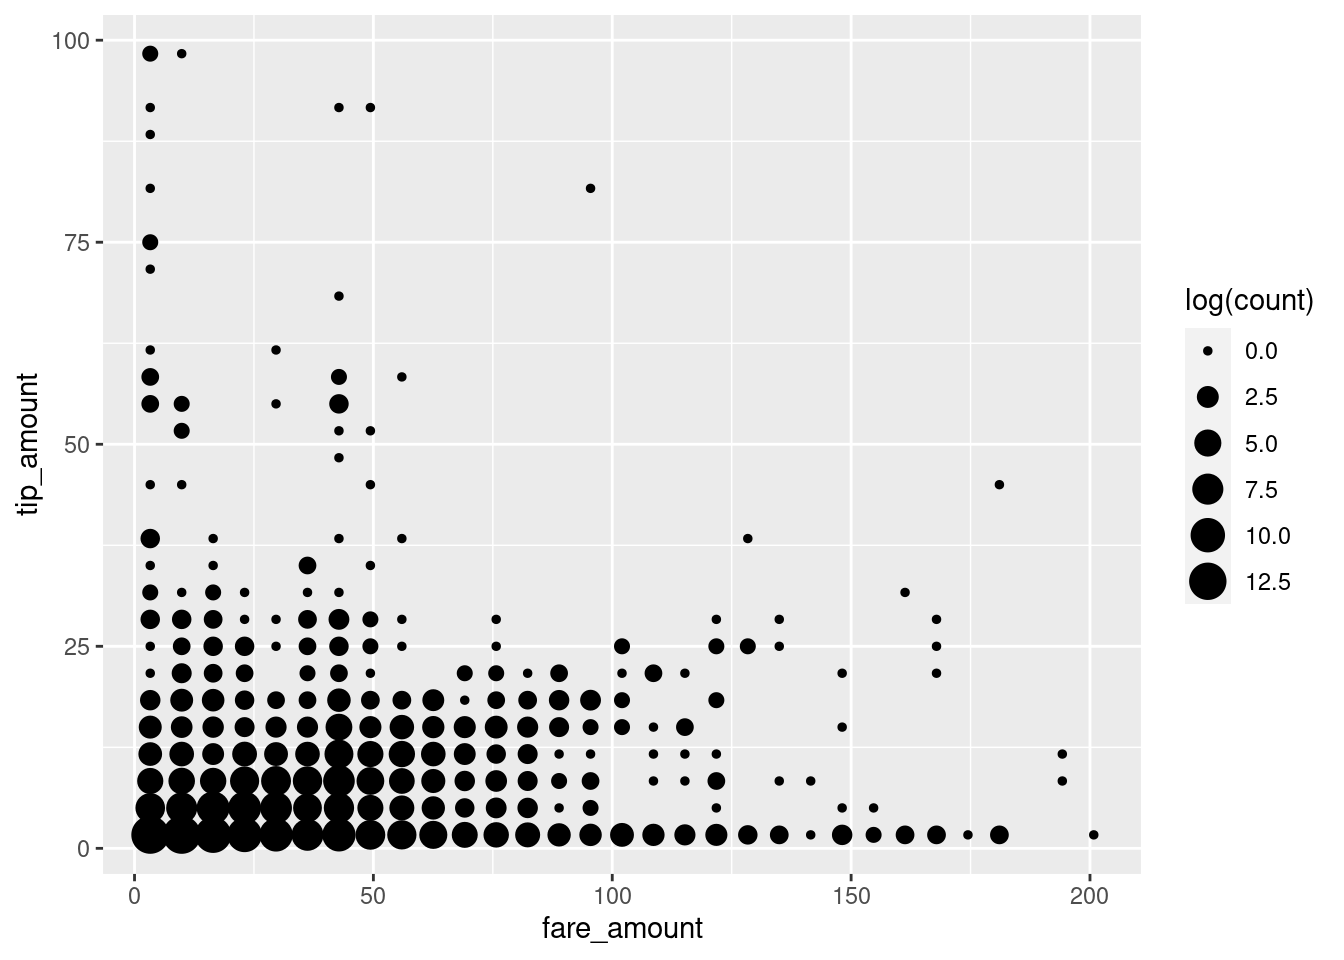
\includegraphics{bigdata_files/figure-latex/unnamed-chunk-178-1.pdf}

The plot suggests that trips involving more than one passenger tend to be paid rather by cash than by credit card.

\hypertarget{high-speed-in-memory-data-aggregation-with-data.table}{%
\section{\texorpdfstring{High-speed in-memory data aggregation with \texttt{data.table}}{High-speed in-memory data aggregation with data.table}}\label{high-speed-in-memory-data-aggregation-with-data.table}}

For large data sets that still fit into RAM, the \texttt{data.table}-package provides very fast and elegant functions to compute aggregate statistics.

\hypertarget{data-import-3}{%
\subsubsection{Data import}\label{data-import-3}}

We use the already familiar \texttt{fread()} to import the same first million observations from the January 2009 taxi trips records.

\begin{Shaded}
\begin{Highlighting}[]
\CommentTok{\# load packages}
\FunctionTok{library}\NormalTok{(data.table)}

\CommentTok{\# import data into RAM (needs around 200MB)}
\NormalTok{taxi }\OtherTok{\textless{}{-}} \FunctionTok{fread}\NormalTok{(}\StringTok{"data/tlc\_trips.csv"}\NormalTok{,}
              \AttributeTok{nrows =} \DecValTok{1000000}\NormalTok{)}
\end{Highlighting}
\end{Shaded}

\hypertarget{data-preparation}{%
\subsubsection{Data preparation}\label{data-preparation}}

We prepare/clean the data as in the \texttt{ff}-approach above.

\begin{Shaded}
\begin{Highlighting}[]
\CommentTok{\# first, we remove the empty vars V8 and V9}
\NormalTok{taxi}\SpecialCharTok{$}\NormalTok{V8 }\OtherTok{\textless{}{-}} \ConstantTok{NULL}
\NormalTok{taxi}\SpecialCharTok{$}\NormalTok{V9 }\OtherTok{\textless{}{-}} \ConstantTok{NULL}


\CommentTok{\# set covariate names according to the data dictionary}
\CommentTok{\# see https://www1.nyc.gov/assets/tlc/downloads/pdf/data\_dictionary\_trip\_records\_yellow.pdf}
\CommentTok{\# note instead of taxizonne ids, long/lat are provided}

\NormalTok{varnames }\OtherTok{\textless{}{-}} \FunctionTok{c}\NormalTok{(}\StringTok{"vendor\_id"}\NormalTok{,}
              \StringTok{"pickup\_time"}\NormalTok{,}
              \StringTok{"dropoff\_time"}\NormalTok{,}
              \StringTok{"passenger\_count"}\NormalTok{,}
              \StringTok{"trip\_distance"}\NormalTok{,}
              \StringTok{"start\_lat"}\NormalTok{,}
              \StringTok{"start\_long"}\NormalTok{,}
              \StringTok{"dest\_lat"}\NormalTok{,}
              \StringTok{"dest\_long"}\NormalTok{,}
              \StringTok{"payment\_type"}\NormalTok{,}
              \StringTok{"fare\_amount"}\NormalTok{,}
              \StringTok{"extra"}\NormalTok{,}
              \StringTok{"mta\_tax"}\NormalTok{,}
              \StringTok{"tip\_amount"}\NormalTok{,}
              \StringTok{"tolls\_amount"}\NormalTok{,}
              \StringTok{"total\_amount"}\NormalTok{)}
\FunctionTok{names}\NormalTok{(taxi) }\OtherTok{\textless{}{-}}\NormalTok{ varnames}

\CommentTok{\# clean the factor levels}
\NormalTok{taxi}\SpecialCharTok{$}\NormalTok{payment\_type }\OtherTok{\textless{}{-}} \FunctionTok{tolower}\NormalTok{(taxi}\SpecialCharTok{$}\NormalTok{payment\_type)}
\NormalTok{taxi}\SpecialCharTok{$}\NormalTok{payment\_type }\OtherTok{\textless{}{-}} \FunctionTok{factor}\NormalTok{(taxi}\SpecialCharTok{$}\NormalTok{payment\_type, }\AttributeTok{levels =} \FunctionTok{unique}\NormalTok{(taxi}\SpecialCharTok{$}\NormalTok{payment\_type))     }
\end{Highlighting}
\end{Shaded}

Note the simpler syntax of essentially doing the same thing, but all in-memory.

\hypertarget{data.table-syntax-for-split-apply-combine-operations}{%
\subsubsection{\texorpdfstring{\texttt{data.table}-syntax for `split-apply-combine' operations}{data.table-syntax for `split-apply-combine' operations}}\label{data.table-syntax-for-split-apply-combine-operations}}

With the \texttt{{[}{]}}-syntax we index/subset usual \texttt{data.frame} objects in R. When working with \texttt{data.table}s, much more can be done in the step of `sub-setting' the frame.\footnote{See \url{https://cran.r-project.org/web/packages/data.table/vignettes/datatable-intro.html} for a detailed introduction to the syntax.}

For example, we can directly compute on columns.

\begin{Shaded}
\begin{Highlighting}[]
\NormalTok{taxi[, }\FunctionTok{mean}\NormalTok{(tip\_amount}\SpecialCharTok{/}\NormalTok{total\_amount)]}
\end{Highlighting}
\end{Shaded}

\begin{verbatim}
## [1] 0.03452
\end{verbatim}

Moreover, in the same step, we can `split' the rows \emph{by} specific groups and apply the function to each subset.

\begin{Shaded}
\begin{Highlighting}[]
\NormalTok{taxi[, .(}\AttributeTok{percent\_tip =} \FunctionTok{mean}\NormalTok{((tip\_amount}\SpecialCharTok{/}\NormalTok{total\_amount)}\SpecialCharTok{*}\DecValTok{100}\NormalTok{)), by }\OtherTok{=}\NormalTok{ payment\_type]}
\end{Highlighting}
\end{Shaded}

\begin{verbatim}
##    payment_type percent_tip
## 1:         cash    0.005978
## 2:       credit   16.004173
## 3:    no charge    0.040433
## 4:      dispute    0.045660
\end{verbatim}

Similarly, we can use \texttt{data.table}'s \texttt{dcast()} for cross-tabulation-like operations.

\begin{Shaded}
\begin{Highlighting}[]
\FunctionTok{dcast}\NormalTok{(taxi[payment\_type }\SpecialCharTok{\%in\%} \FunctionTok{c}\NormalTok{(}\StringTok{"credit"}\NormalTok{, }\StringTok{"cash"}\NormalTok{)],}
\NormalTok{      passenger\_count}\SpecialCharTok{\textasciitilde{}}\NormalTok{payment\_type, }
      \AttributeTok{fun.aggregate =}\NormalTok{ length,}
      \AttributeTok{value.var =} \StringTok{"vendor\_id"}\NormalTok{)}
\end{Highlighting}
\end{Shaded}

\begin{verbatim}
##    passenger_count   cash credit
## 1:               0     44      2
## 2:               1 516828 149990
## 3:               2 133468  32891
## 4:               3  36439   7847
## 5:               4  17901   2909
## 6:               5  73027  20688
## 7:               6   3588   1097
\end{verbatim}

\hypertarget{big-data-visualization}{%
\chapter{(Big) Data Visualization}\label{big-data-visualization}}

\hypertarget{data-exploration-with-ggplot2}{%
\section{\texorpdfstring{Data exploration with \texttt{ggplot2}}{Data exploration with ggplot2}}\label{data-exploration-with-ggplot2}}

In this tutorial we will work with the TLC data used in the data aggregation session. The raw data consists of several monthly CSV-files and can be downloaded via the \href{https://www1.nyc.gov/site/tlc/about/tlc-trip-record-data.page}{TLC's website}. Again, we work only with the first million observations.

In order to better understand the large data set at hand (particularly regarding the determinants of tips paid) we use \texttt{ggplot2} to visualize some key aspects of the data.

First, let's look at the raw relationship between fare paid and the tip paid. We set up the canvas with \texttt{ggplot}.

\begin{Shaded}
\begin{Highlighting}[]
\CommentTok{\# load packages}
\FunctionTok{library}\NormalTok{(ggplot2)}

\CommentTok{\# set up the canvas}
\NormalTok{taxiplot }\OtherTok{\textless{}{-}} \FunctionTok{ggplot}\NormalTok{(taxi, }\FunctionTok{aes}\NormalTok{(}\AttributeTok{y=}\NormalTok{tip\_amount, }\AttributeTok{x=}\NormalTok{ fare\_amount)) }
\NormalTok{taxiplot}
\end{Highlighting}
\end{Shaded}

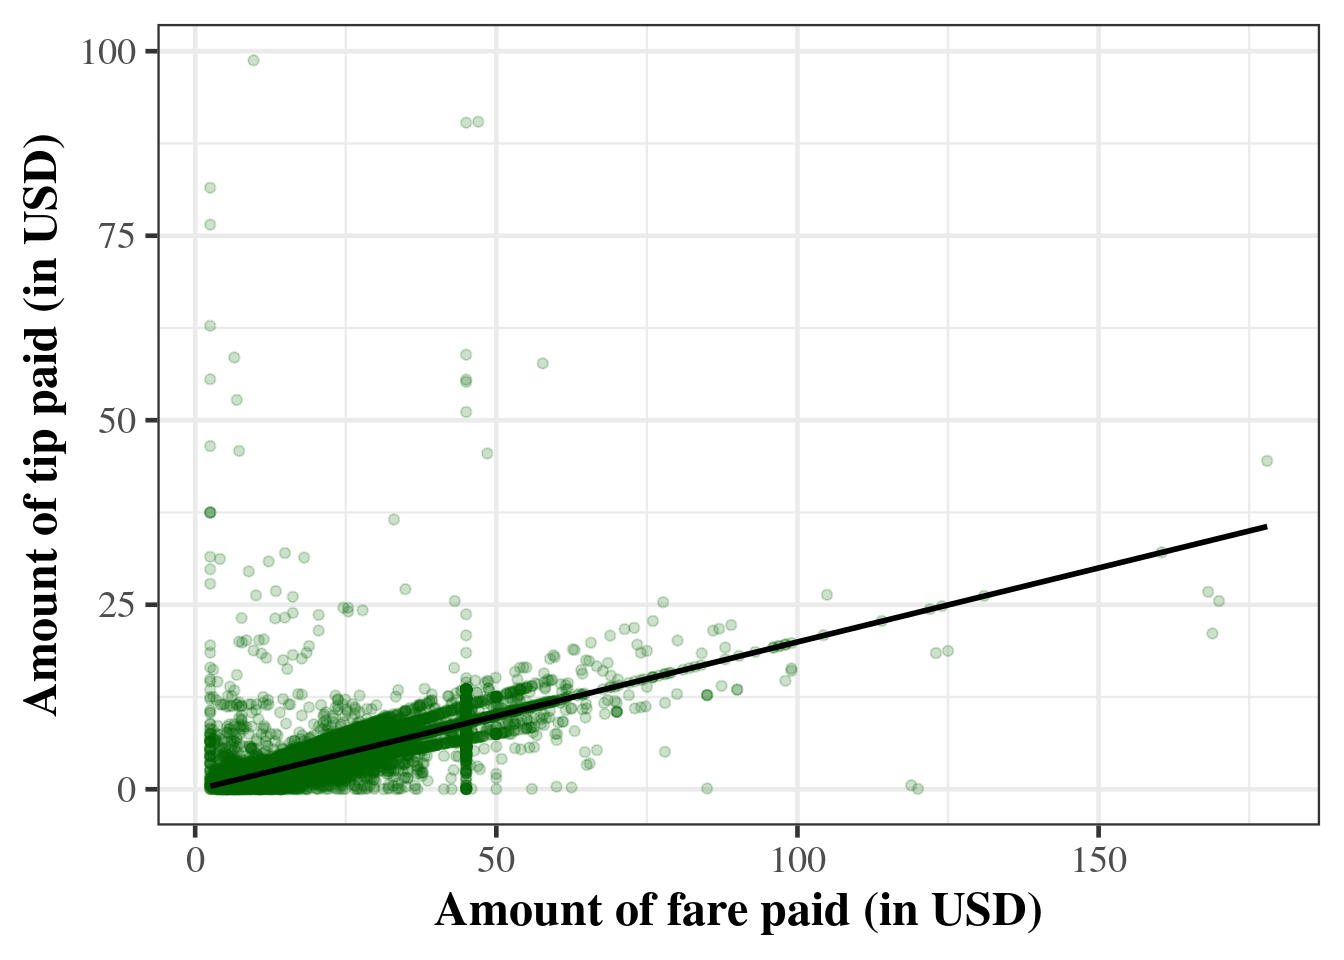
\includegraphics{bigdata_files/figure-latex/unnamed-chunk-186-1.pdf}

Now we visualize the co-distribution of the two variables with a simple scatter-plot.

\begin{Shaded}
\begin{Highlighting}[]
\CommentTok{\# simple x/y plot}
\NormalTok{taxiplot }\SpecialCharTok{+}
     \FunctionTok{geom\_point}\NormalTok{()}
\end{Highlighting}
\end{Shaded}

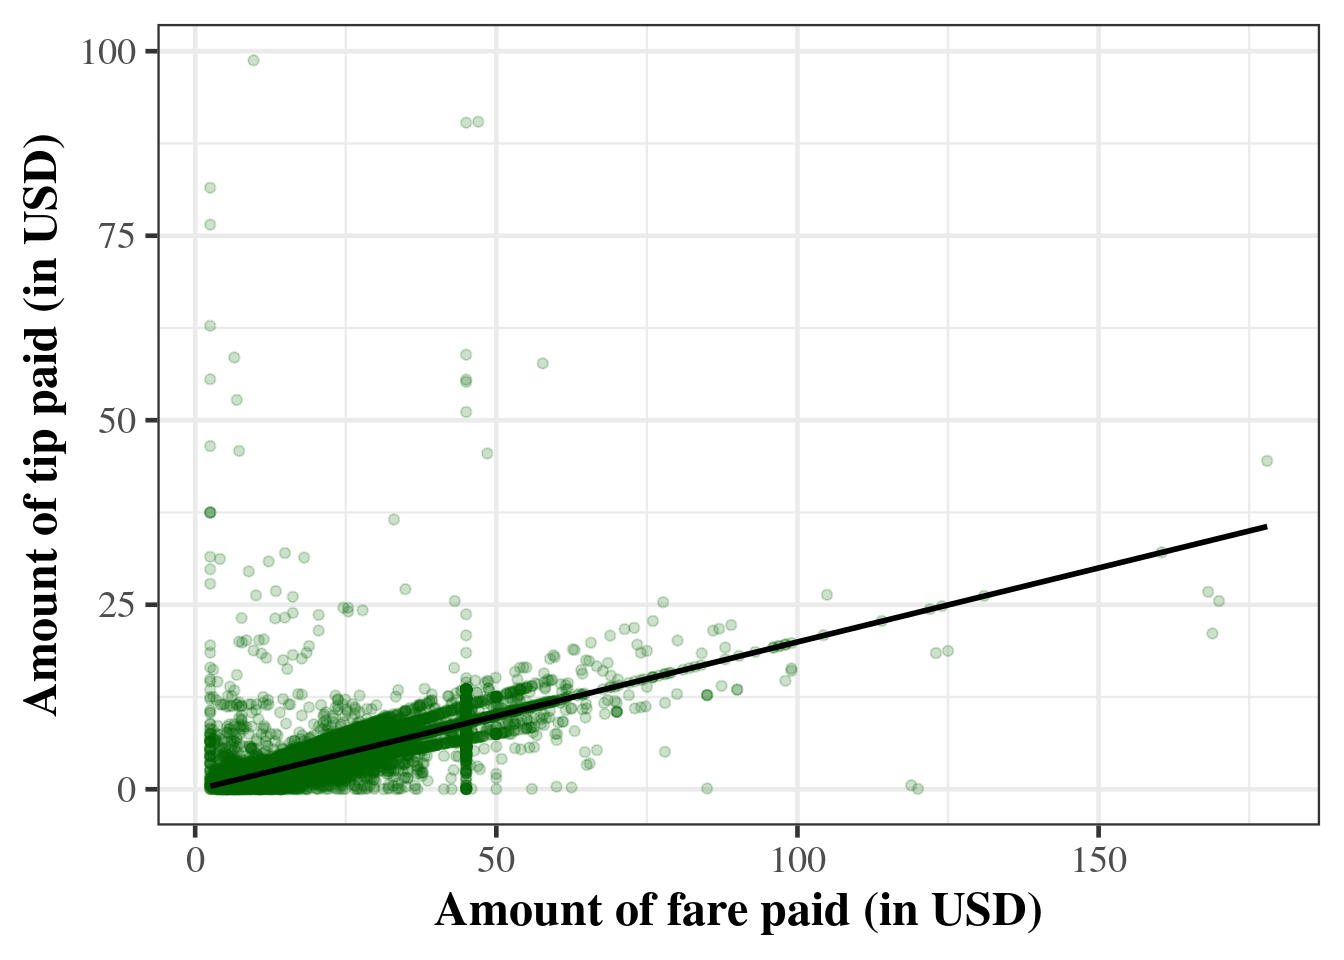
\includegraphics{bigdata_files/figure-latex/unnamed-chunk-187-1.pdf}

Note that this took quite a while, as R had to literally plot one million dots on the canvas. Moreover many dots fall within the same area, making it impossible to recognize how much mass there actually is. This is typical for visualization exercises with large data sets. One way to improve this, is by making the dots more transparent by setting the \texttt{alpha} parameter.

\begin{Shaded}
\begin{Highlighting}[]
\CommentTok{\# simple x/y plot}
\NormalTok{taxiplot }\SpecialCharTok{+}
     \FunctionTok{geom\_point}\NormalTok{(}\AttributeTok{alpha=}\FloatTok{0.2}\NormalTok{)}
\end{Highlighting}
\end{Shaded}

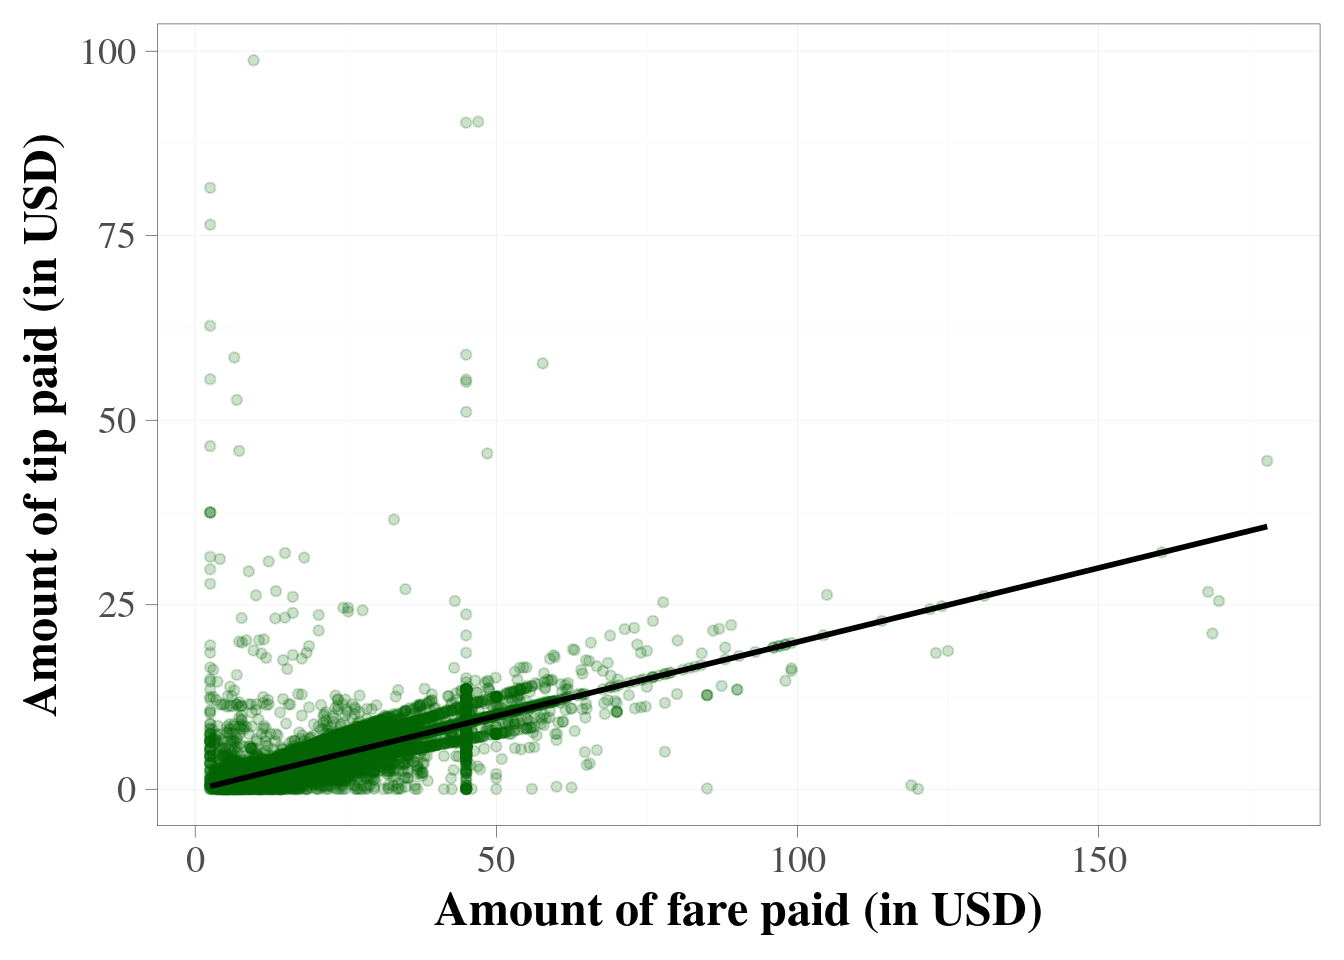
\includegraphics{bigdata_files/figure-latex/unnamed-chunk-188-1.pdf}

Alternatively, we can compute two-dimensional bins. Thereby, the canvas is split into rectangles and the number of observations falling into each respective rectangle is computed. The visualization is based on plotting the rectangles with counts greater than 0 and the shading of the rectangles indicates the count values.

\begin{Shaded}
\begin{Highlighting}[]
\CommentTok{\# 2{-}dimensional bins}
\NormalTok{taxiplot }\SpecialCharTok{+}
     \FunctionTok{geom\_bin2d}\NormalTok{()}
\end{Highlighting}
\end{Shaded}

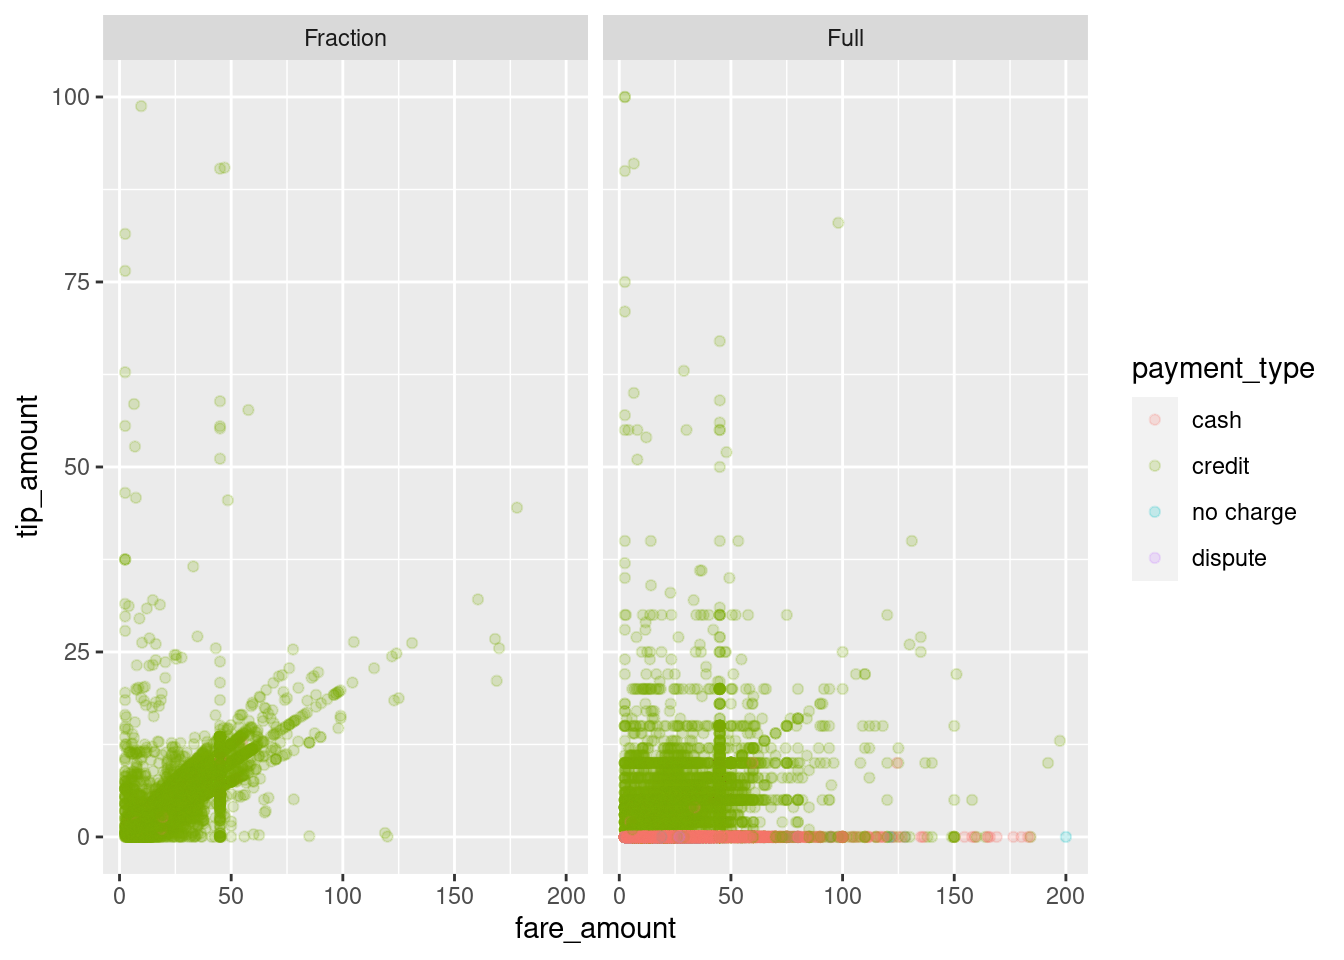
\includegraphics{bigdata_files/figure-latex/unnamed-chunk-189-1.pdf}

A large part of the tip/fare observations seem to be in the very lower-left corner of the pane, while most other trips seem to be evenly distributed. However, we fail to see slighter differences in this visualization. In order to reduce the dominance of the 2d-bins with very high counts, we display the natural logarithm of counts and display the bins as points.

\begin{Shaded}
\begin{Highlighting}[]
\CommentTok{\# 2{-}dimensional bins}
\NormalTok{taxiplot }\SpecialCharTok{+}
     \FunctionTok{stat\_bin\_2d}\NormalTok{(}\AttributeTok{geom=}\StringTok{"point"}\NormalTok{,}
                 \AttributeTok{mapping=} \FunctionTok{aes}\NormalTok{(}\AttributeTok{size =} \FunctionTok{log}\NormalTok{(..count..))) }\SpecialCharTok{+}
     \FunctionTok{guides}\NormalTok{(}\AttributeTok{fill =} \ConstantTok{FALSE}\NormalTok{)}
\end{Highlighting}
\end{Shaded}

\begin{verbatim}
## Warning: `guides(<scale> = FALSE)` is deprecated.
## Please use `guides(<scale> = "none")` instead.
\end{verbatim}

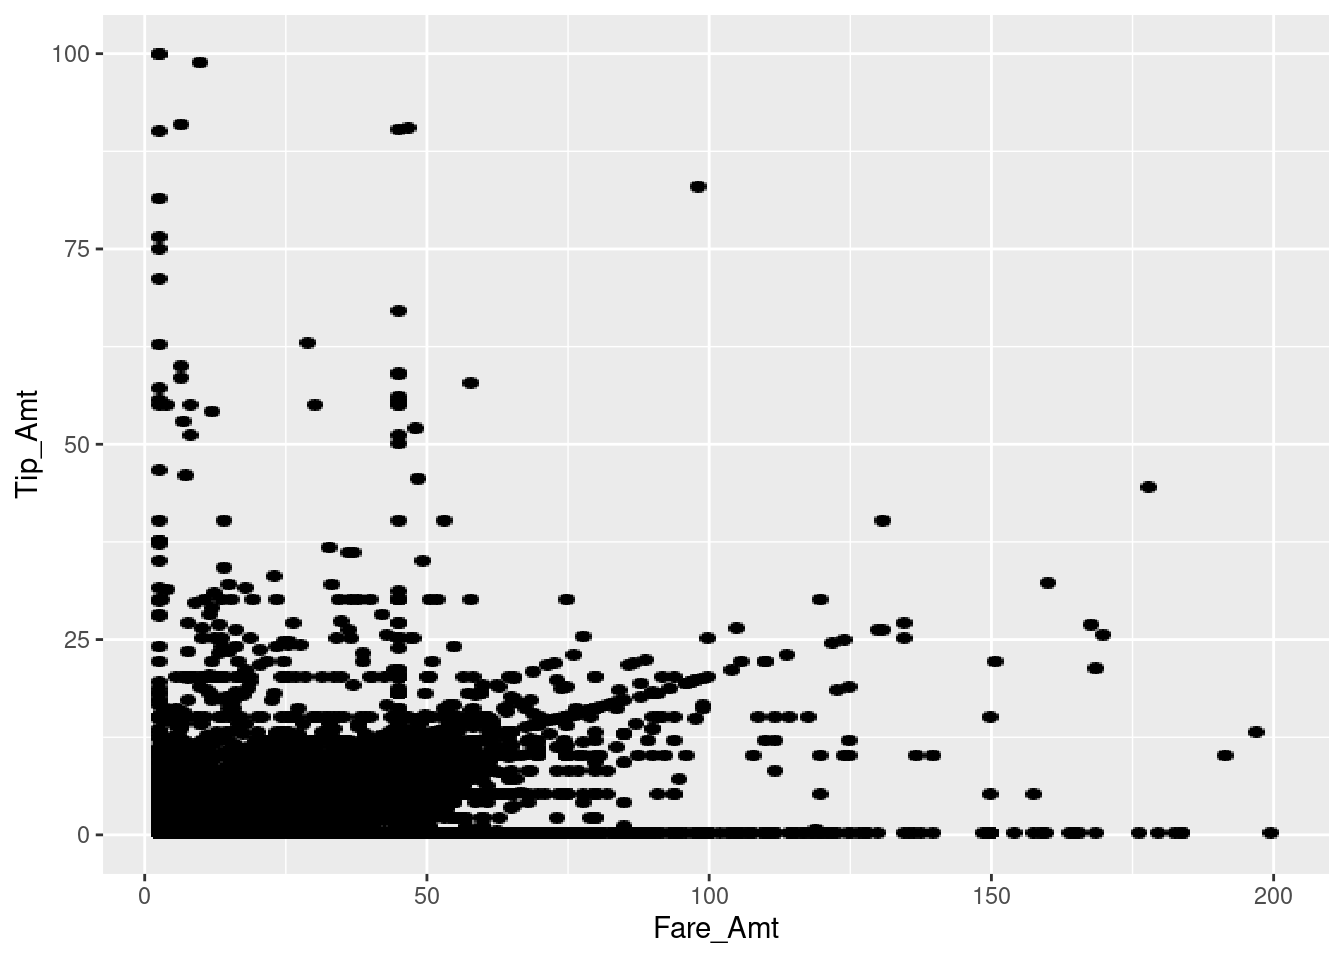
\includegraphics{bigdata_files/figure-latex/unnamed-chunk-190-1.pdf}

We note that there are many cases with very low fare amounts, many cases with no or hardly any tip, and quite a lot of cases with very high tip amounts (in relation to the rather low fare amount). In the following, we dissect this picture by having a closer look at `typical' tip amounts and whether they differ by type of payment.

\begin{Shaded}
\begin{Highlighting}[]
\CommentTok{\# compute frequency of per tip amount and payment method}
\NormalTok{taxi[, n\_same\_tip}\SpecialCharTok{:}\ErrorTok{=}\NormalTok{ .N, by}\OtherTok{=} \FunctionTok{c}\NormalTok{(}\StringTok{"tip\_amount"}\NormalTok{, }\StringTok{"payment\_type"}\NormalTok{)]}
\NormalTok{frequencies }\OtherTok{\textless{}{-}} \FunctionTok{unique}\NormalTok{(taxi[payment\_type }\SpecialCharTok{\%in\%} \FunctionTok{c}\NormalTok{(}\StringTok{"credit"}\NormalTok{, }\StringTok{"cash"}\NormalTok{),}
                           \FunctionTok{c}\NormalTok{(}\StringTok{"n\_same\_tip"}\NormalTok{, }\StringTok{"tip\_amount"}\NormalTok{, }\StringTok{"payment\_type"}\NormalTok{)][}\FunctionTok{order}\NormalTok{(n\_same\_tip, }\AttributeTok{decreasing =} \ConstantTok{TRUE}\NormalTok{)])}


\CommentTok{\# plot top 20 frequent tip amounts}
\NormalTok{fare }\OtherTok{\textless{}{-}} \FunctionTok{ggplot}\NormalTok{(}\AttributeTok{data =}\NormalTok{ frequencies[}\DecValTok{1}\SpecialCharTok{:}\DecValTok{20}\NormalTok{], }\FunctionTok{aes}\NormalTok{(}\AttributeTok{x =} \FunctionTok{factor}\NormalTok{(tip\_amount), }\AttributeTok{y =}\NormalTok{ n\_same\_tip)) }
\NormalTok{fare }\SpecialCharTok{+} \FunctionTok{geom\_bar}\NormalTok{(}\AttributeTok{stat =} \StringTok{"identity"}\NormalTok{) }
\end{Highlighting}
\end{Shaded}

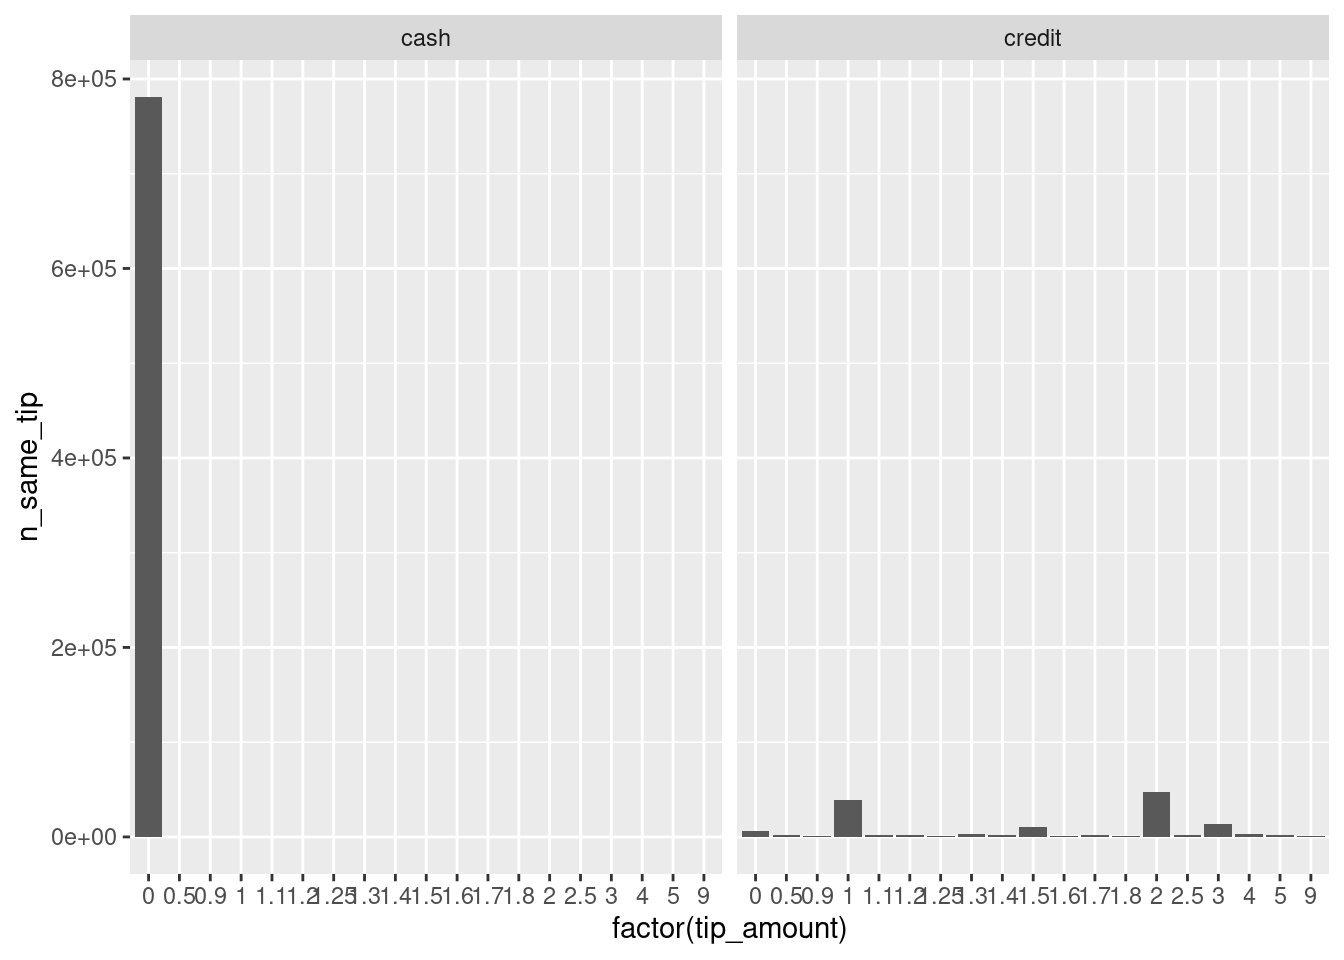
\includegraphics{bigdata_files/figure-latex/unnamed-chunk-191-1.pdf}

Indeed, paying no tip at all is quite frequent, overall.\footnote{Or, could there be another explanation for this pattern in the data?} The bar plot also indicates that there seem to be some `focal points' in the amount of tips paid. Clearly, paying one USD or two USD is more common than paying fractions. However, fractions of dollars might be more likely if tips are paid in cash and customers simply add some loose change to the fare amount paid.

\begin{Shaded}
\begin{Highlighting}[]
\NormalTok{fare }\SpecialCharTok{+} \FunctionTok{geom\_bar}\NormalTok{(}\AttributeTok{stat =} \StringTok{"identity"}\NormalTok{) }\SpecialCharTok{+} 
     \FunctionTok{facet\_wrap}\NormalTok{(}\StringTok{"payment\_type"}\NormalTok{) }
\end{Highlighting}
\end{Shaded}

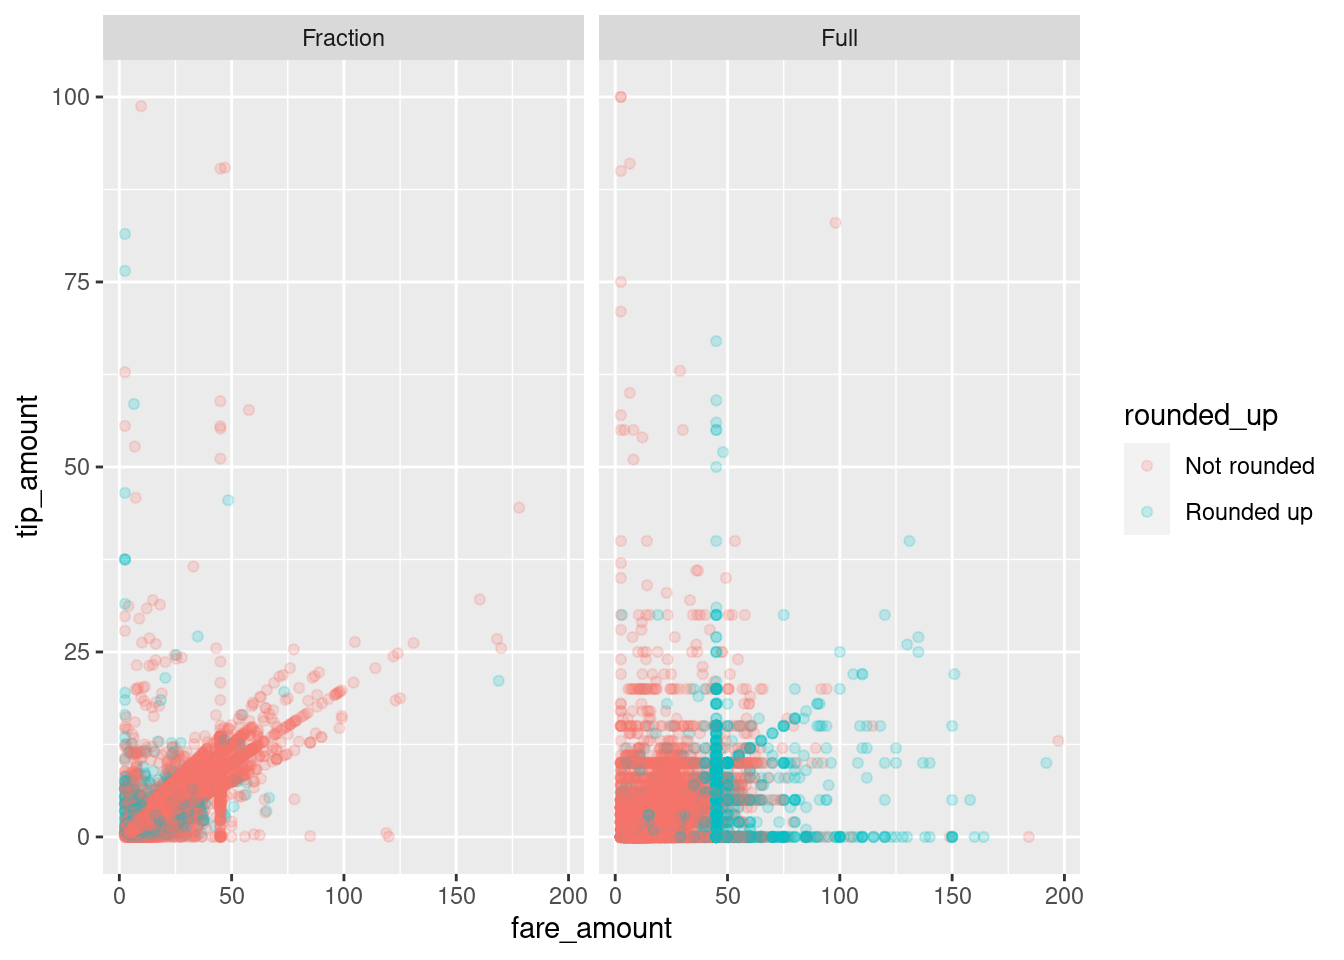
\includegraphics{bigdata_files/figure-latex/unnamed-chunk-192-1.pdf}

Clearly, it looks like trips paid in cash tend not to be tipped (at least in this subsample).

Let's try to tease this information out of the initial points plot. Trips paid in cash are often not tipped, we thus should indicate the payment method. Moreover, tips paid in full dollar amounts might indicate a habit.

\begin{Shaded}
\begin{Highlighting}[]
\CommentTok{\# indicate natural numbers}
\NormalTok{taxi[, dollar\_paid }\SpecialCharTok{:}\ErrorTok{=} \FunctionTok{ifelse}\NormalTok{(tip\_amount }\SpecialCharTok{==} \FunctionTok{round}\NormalTok{(tip\_amount,}\DecValTok{0}\NormalTok{), }\StringTok{"Full"}\NormalTok{, }\StringTok{"Fraction"}\NormalTok{),]}


\CommentTok{\# extended x/y plot}
\NormalTok{taxiplot }\SpecialCharTok{+}
     \FunctionTok{geom\_point}\NormalTok{(}\AttributeTok{alpha=}\FloatTok{0.2}\NormalTok{, }\FunctionTok{aes}\NormalTok{(}\AttributeTok{color=}\NormalTok{payment\_type)) }\SpecialCharTok{+}
     \FunctionTok{facet\_wrap}\NormalTok{(}\StringTok{"dollar\_paid"}\NormalTok{)}
\end{Highlighting}
\end{Shaded}

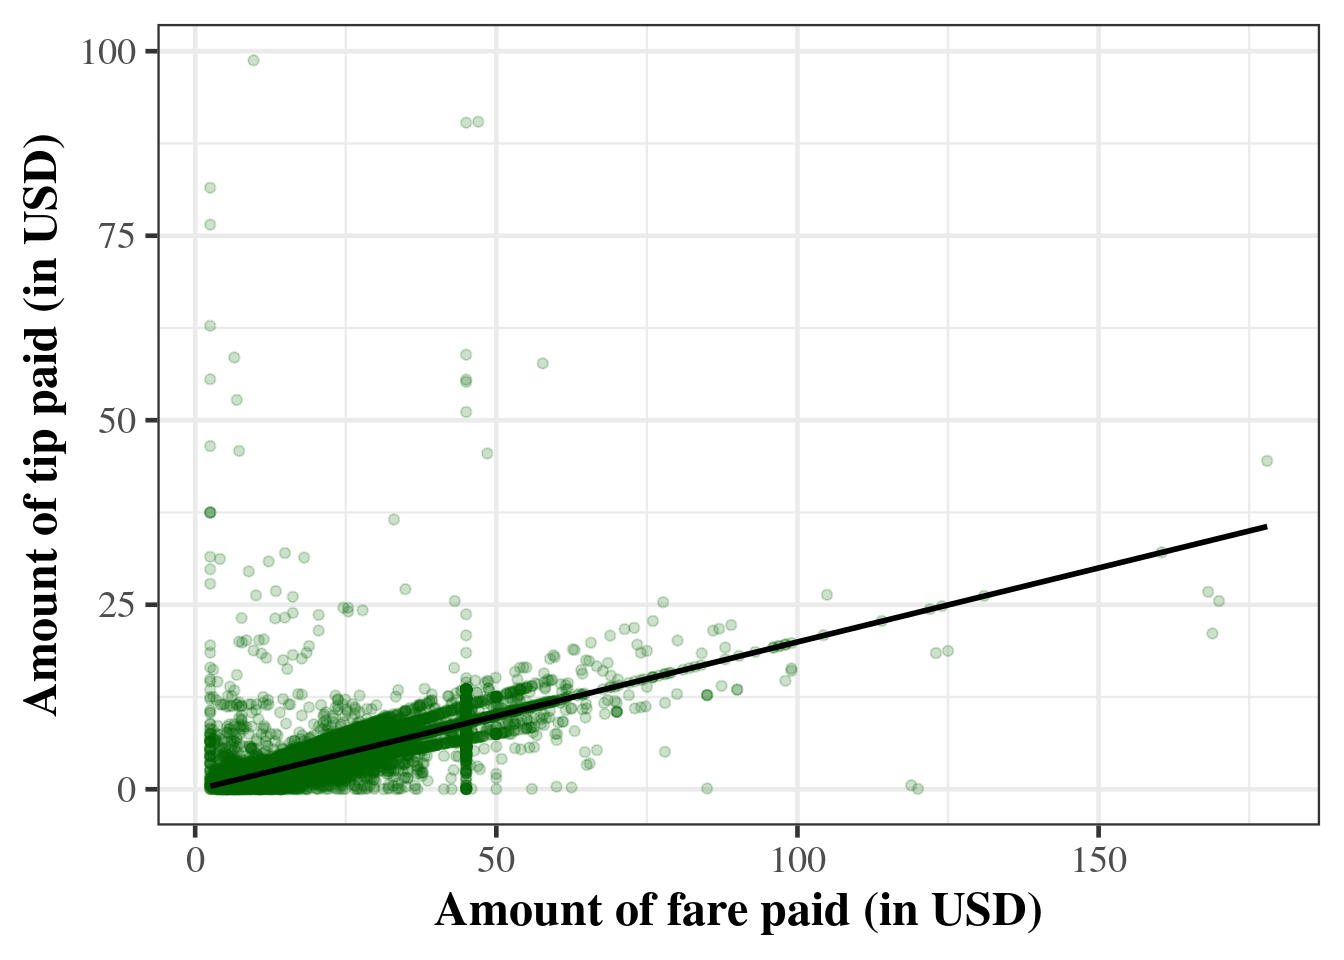
\includegraphics{bigdata_files/figure-latex/unnamed-chunk-193-1.pdf}

Now the picture is getting clearer. Paying tip seems to follow certain rules of thumb. Certain fixed amounts tend to be paid independent of the fare amount (visible in the straight lines of dots on the right-hand panel). At the same time, the pattern in the left panel indicates another habit: computing the amount of tip as a linear function of the total fare amount (`pay 10\% tip'). A third habit might be to determine the amount of tip by `rounding up' the total amount paid. In the following, we try to tease the latter out, only focusing on credit card payments.

\begin{Shaded}
\begin{Highlighting}[]
\NormalTok{taxi[, rounded\_up }\SpecialCharTok{:}\ErrorTok{=} \FunctionTok{ifelse}\NormalTok{(fare\_amount }\SpecialCharTok{+}\NormalTok{ tip\_amount }\SpecialCharTok{==} \FunctionTok{round}\NormalTok{(fare\_amount }\SpecialCharTok{+}\NormalTok{ tip\_amount, }\DecValTok{0}\NormalTok{),}
                            \StringTok{"Rounded up"}\NormalTok{,}
                            \StringTok{"Not rounded"}\NormalTok{)]}
\CommentTok{\# extended x/y plot}
\NormalTok{taxiplot }\SpecialCharTok{+}
     \FunctionTok{geom\_point}\NormalTok{(}\AttributeTok{data=}\NormalTok{ taxi[payment\_type }\SpecialCharTok{==} \StringTok{"credit"}\NormalTok{],}
                \AttributeTok{alpha=}\FloatTok{0.2}\NormalTok{, }\FunctionTok{aes}\NormalTok{(}\AttributeTok{color=}\NormalTok{rounded\_up)) }\SpecialCharTok{+}
     \FunctionTok{facet\_wrap}\NormalTok{(}\StringTok{"dollar\_paid"}\NormalTok{)}
\end{Highlighting}
\end{Shaded}

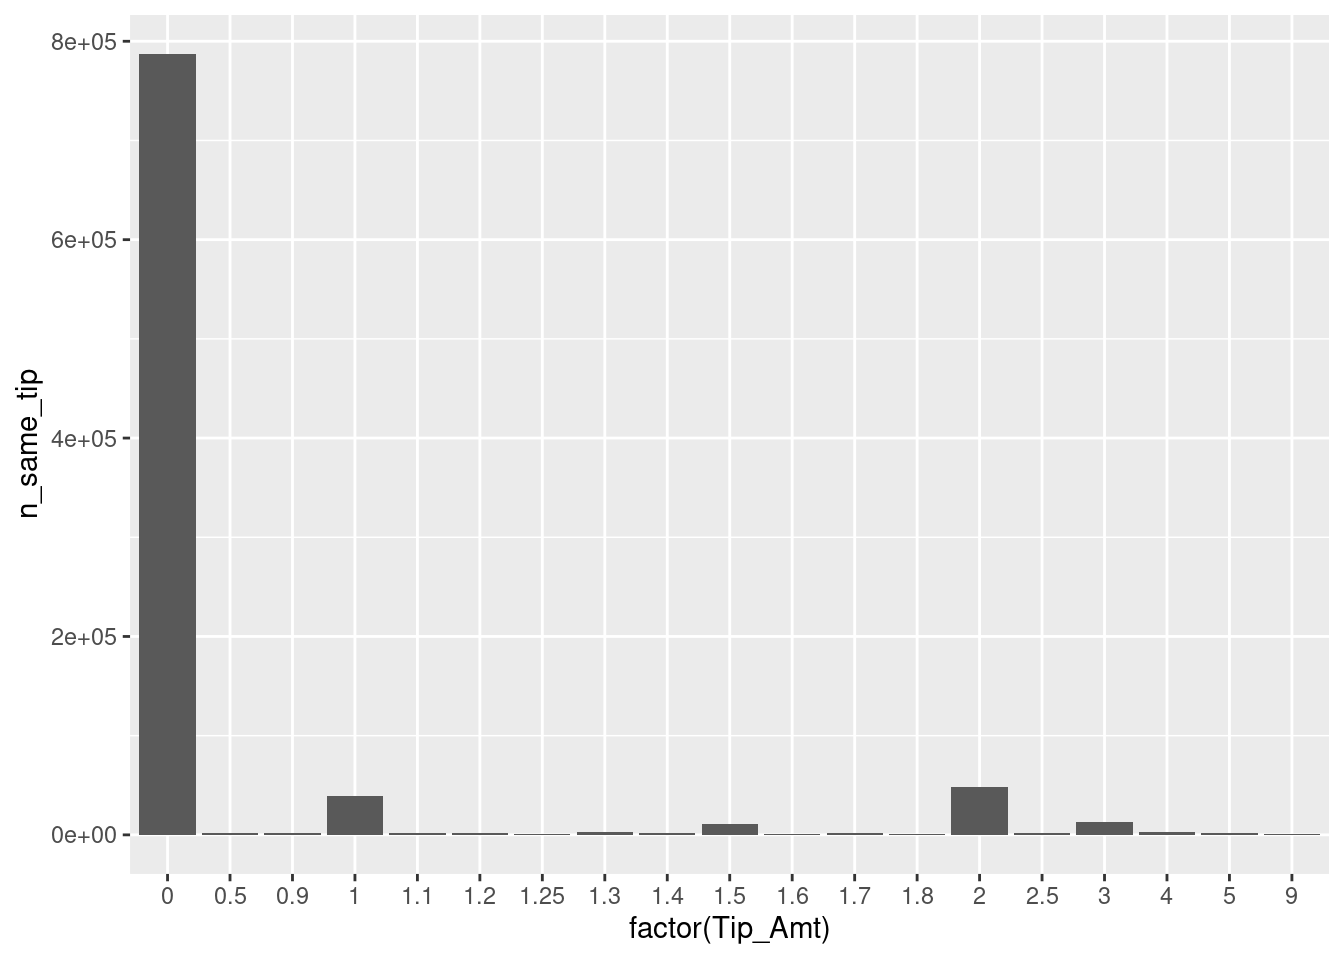
\includegraphics{bigdata_files/figure-latex/unnamed-chunk-194-1.pdf}

Now we can start modelling. A reasonable first shot is to model the tip amount as a linear function of the fare amount, conditional on the no-zero tip amounts paid as fractions of a dollar.

\begin{Shaded}
\begin{Highlighting}[]
\NormalTok{modelplot }\OtherTok{\textless{}{-}} \FunctionTok{ggplot}\NormalTok{(}\AttributeTok{data=}\NormalTok{ taxi[payment\_type }\SpecialCharTok{==} \StringTok{"credit"} \SpecialCharTok{\&}\NormalTok{ dollar\_paid }\SpecialCharTok{==} \StringTok{"Fraction"} \SpecialCharTok{\&} \DecValTok{0} \SpecialCharTok{\textless{}}\NormalTok{ tip\_amount],}
                    \FunctionTok{aes}\NormalTok{(}\AttributeTok{x =}\NormalTok{ fare\_amount, }\AttributeTok{y =}\NormalTok{ tip\_amount))}
\NormalTok{modelplot }\SpecialCharTok{+}
     \FunctionTok{geom\_point}\NormalTok{(}\AttributeTok{alpha=}\FloatTok{0.2}\NormalTok{, }\AttributeTok{colour=}\StringTok{"darkgreen"}\NormalTok{) }\SpecialCharTok{+}
     \FunctionTok{geom\_smooth}\NormalTok{(}\AttributeTok{method =} \StringTok{"lm"}\NormalTok{, }\AttributeTok{colour =} \StringTok{"black"}\NormalTok{)}
\end{Highlighting}
\end{Shaded}

\begin{verbatim}
## `geom_smooth()` using formula 'y ~ x'
\end{verbatim}

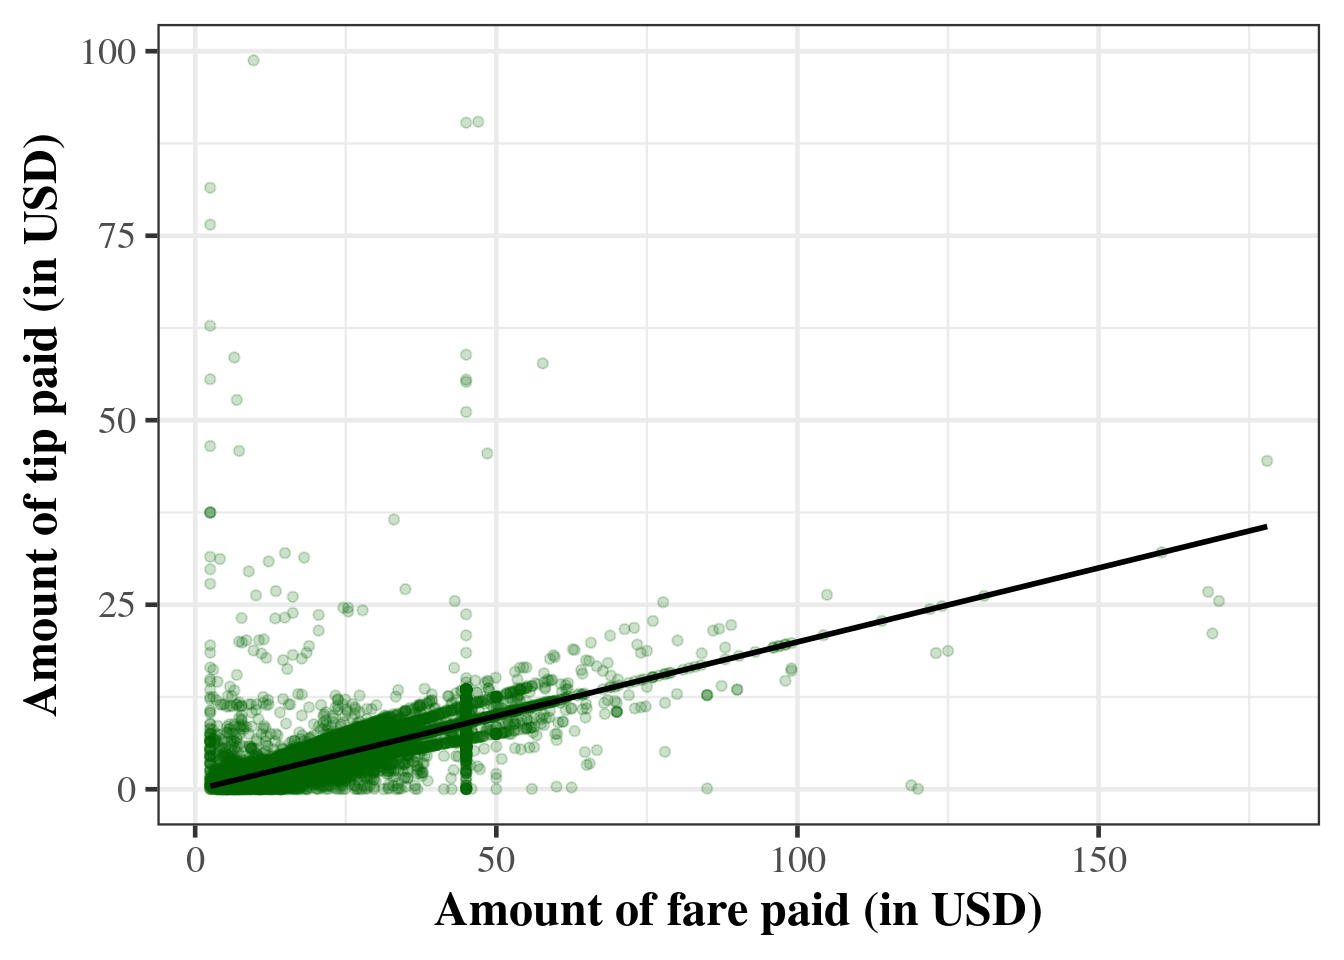
\includegraphics{bigdata_files/figure-latex/unnamed-chunk-195-1.pdf}

Finally, we prepare the plot for reporting. \texttt{ggplot2} provides several predefined `themes' for plots which define all kind of aspects of a plot (background color, line colors, font size etc.). The easiest way to tweak the design of your final plot in a certain direction is to just add such a pre-defined theme at the end of your plot. Some of the pre-defined themes allow you to change a few aspects such as the font type and the base size of all the texts in the plot (labels and tick numbers etc.). Here, we use the \texttt{theme\_bw()}, increase the font size and switch to serif-type font. \texttt{theme\_bw()} is one of the complete themes already shipped with the basic \texttt{ggplot2} installation.\footnote{See \href{https://ggplot2.tidyverse.org/reference/ggtheme.html}{the ggplot2 documentation} for a list of all pre-defined themes shipped with the basic installation.} Many more themes can be found in additional R packages (see, for example, the \href{https://cran.r-project.org/web/packages/ggthemes/index.html}{\texttt{ggthemes} package}).

\begin{Shaded}
\begin{Highlighting}[]
\NormalTok{modelplot }\OtherTok{\textless{}{-}} \FunctionTok{ggplot}\NormalTok{(}\AttributeTok{data=}\NormalTok{ taxi[payment\_type }\SpecialCharTok{==} \StringTok{"credit"} \SpecialCharTok{\&}\NormalTok{ dollar\_paid }\SpecialCharTok{==} \StringTok{"Fraction"} \SpecialCharTok{\&} \DecValTok{0} \SpecialCharTok{\textless{}}\NormalTok{ tip\_amount],}
                    \FunctionTok{aes}\NormalTok{(}\AttributeTok{x =}\NormalTok{ fare\_amount, }\AttributeTok{y =}\NormalTok{ tip\_amount))}
\NormalTok{modelplot }\SpecialCharTok{+}
     \FunctionTok{geom\_point}\NormalTok{(}\AttributeTok{alpha=}\FloatTok{0.2}\NormalTok{, }\AttributeTok{colour=}\StringTok{"darkgreen"}\NormalTok{) }\SpecialCharTok{+}
     \FunctionTok{geom\_smooth}\NormalTok{(}\AttributeTok{method =} \StringTok{"lm"}\NormalTok{, }\AttributeTok{colour =} \StringTok{"black"}\NormalTok{) }\SpecialCharTok{+}
     \FunctionTok{ylab}\NormalTok{(}\StringTok{"Amount of tip paid (in USD)"}\NormalTok{) }\SpecialCharTok{+}
     \FunctionTok{xlab}\NormalTok{(}\StringTok{"Amount of fare paid (in USD)"}\NormalTok{) }\SpecialCharTok{+}
     \FunctionTok{theme\_bw}\NormalTok{(}\AttributeTok{base\_size =} \DecValTok{18}\NormalTok{, }\AttributeTok{base\_family =} \StringTok{"serif"}\NormalTok{)}
\end{Highlighting}
\end{Shaded}

\begin{verbatim}
## `geom_smooth()` using formula 'y ~ x'
\end{verbatim}

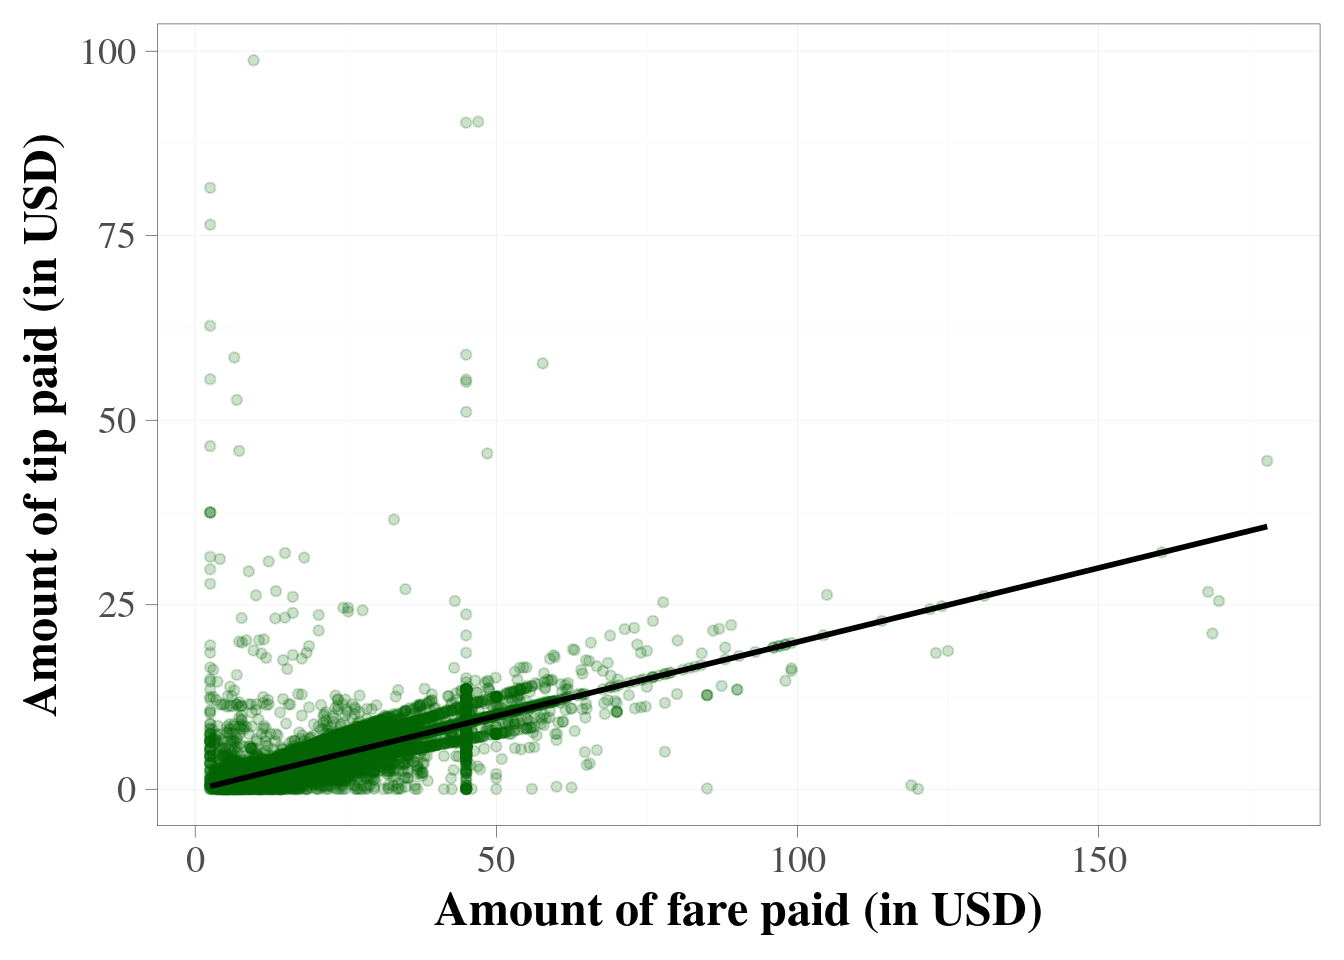
\includegraphics{bigdata_files/figure-latex/unnamed-chunk-196-1.pdf}

\hypertarget{excursus-modify-and-create-themes}{%
\section{Excursus: modify and create themes}\label{excursus-modify-and-create-themes}}

Apart from using pre-defined themes as illustrated above, we can use the \texttt{theme()} function to further modify the design of a plot. For example, we can print the axis labels (`axis titles') in bold.

\begin{Shaded}
\begin{Highlighting}[]
\NormalTok{modelplot }\OtherTok{\textless{}{-}} \FunctionTok{ggplot}\NormalTok{(}\AttributeTok{data=}\NormalTok{ taxi[payment\_type }\SpecialCharTok{==} \StringTok{"credit"} \SpecialCharTok{\&}\NormalTok{ dollar\_paid }\SpecialCharTok{==} \StringTok{"Fraction"} \SpecialCharTok{\&} \DecValTok{0} \SpecialCharTok{\textless{}}\NormalTok{ tip\_amount],}
                    \FunctionTok{aes}\NormalTok{(}\AttributeTok{x =}\NormalTok{ fare\_amount, }\AttributeTok{y =}\NormalTok{ tip\_amount))}
\NormalTok{modelplot }\SpecialCharTok{+}
     \FunctionTok{geom\_point}\NormalTok{(}\AttributeTok{alpha=}\FloatTok{0.2}\NormalTok{, }\AttributeTok{colour=}\StringTok{"darkgreen"}\NormalTok{) }\SpecialCharTok{+}
     \FunctionTok{geom\_smooth}\NormalTok{(}\AttributeTok{method =} \StringTok{"lm"}\NormalTok{, }\AttributeTok{colour =} \StringTok{"black"}\NormalTok{) }\SpecialCharTok{+}
     \FunctionTok{ylab}\NormalTok{(}\StringTok{"Amount of tip paid (in USD)"}\NormalTok{) }\SpecialCharTok{+}
     \FunctionTok{xlab}\NormalTok{(}\StringTok{"Amount of fare paid (in USD)"}\NormalTok{) }\SpecialCharTok{+}
     \FunctionTok{theme\_bw}\NormalTok{(}\AttributeTok{base\_size =} \DecValTok{18}\NormalTok{, }\AttributeTok{base\_family =} \StringTok{"serif"}\NormalTok{) }\SpecialCharTok{+}
     \FunctionTok{theme}\NormalTok{(}\AttributeTok{axis.title =} \FunctionTok{element\_text}\NormalTok{(}\AttributeTok{face=}\StringTok{"bold"}\NormalTok{))}
\end{Highlighting}
\end{Shaded}

\begin{verbatim}
## `geom_smooth()` using formula 'y ~ x'
\end{verbatim}

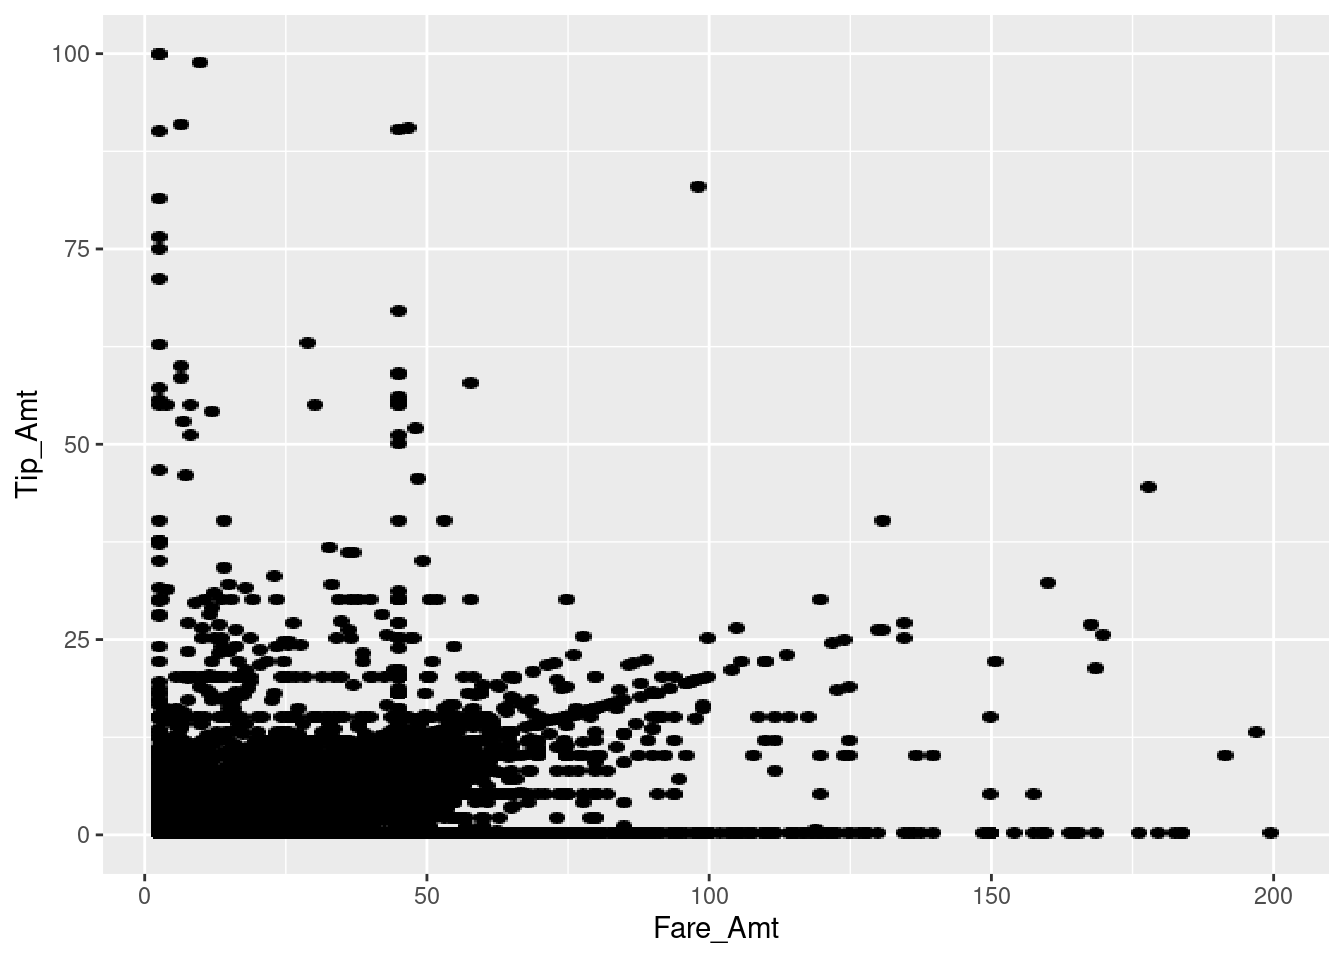
\includegraphics{bigdata_files/figure-latex/unnamed-chunk-197-1.pdf}

There is a large list of plot design aspects that can be modified in this way (see \texttt{?theme()} for details).

\hypertarget{create-your-own-theme-simple-approach}{%
\subsection{Create your own theme: simple approach}\label{create-your-own-theme-simple-approach}}

Extensive design modifications via \texttt{theme()} can involve many lines of code, making your plot code harder to read/understand. In practice, you might want to define your specific theme once and then apply this theme to all of your plots. In order to do so it makes sense to choose one of the existing themes as a basis and then modify its design aspects until you have the design you are looking for. Following the design choices in the examples above, we can create our own \texttt{theme\_my\_serif()} as follows.

\begin{Shaded}
\begin{Highlighting}[]
\CommentTok{\# \textquotesingle{}define\textquotesingle{} a new theme}
\NormalTok{theme\_my\_serif }\OtherTok{\textless{}{-}}      
  \FunctionTok{theme\_bw}\NormalTok{(}\AttributeTok{base\_size =} \DecValTok{18}\NormalTok{, }\AttributeTok{base\_family =} \StringTok{"serif"}\NormalTok{) }\SpecialCharTok{+}
  \FunctionTok{theme}\NormalTok{(}\AttributeTok{axis.title =} \FunctionTok{element\_text}\NormalTok{(}\AttributeTok{face=}\StringTok{"bold"}\NormalTok{))}

\CommentTok{\# apply it }
\NormalTok{modelplot }\SpecialCharTok{+}
     \FunctionTok{geom\_point}\NormalTok{(}\AttributeTok{alpha=}\FloatTok{0.2}\NormalTok{, }\AttributeTok{colour=}\StringTok{"darkgreen"}\NormalTok{) }\SpecialCharTok{+}
     \FunctionTok{geom\_smooth}\NormalTok{(}\AttributeTok{method =} \StringTok{"lm"}\NormalTok{, }\AttributeTok{colour =} \StringTok{"black"}\NormalTok{) }\SpecialCharTok{+}
     \FunctionTok{ylab}\NormalTok{(}\StringTok{"Amount of tip paid (in USD)"}\NormalTok{) }\SpecialCharTok{+}
     \FunctionTok{xlab}\NormalTok{(}\StringTok{"Amount of fare paid (in USD)"}\NormalTok{) }\SpecialCharTok{+}
\NormalTok{  theme\_my\_serif}
\end{Highlighting}
\end{Shaded}

\begin{verbatim}
## `geom_smooth()` using formula 'y ~ x'
\end{verbatim}

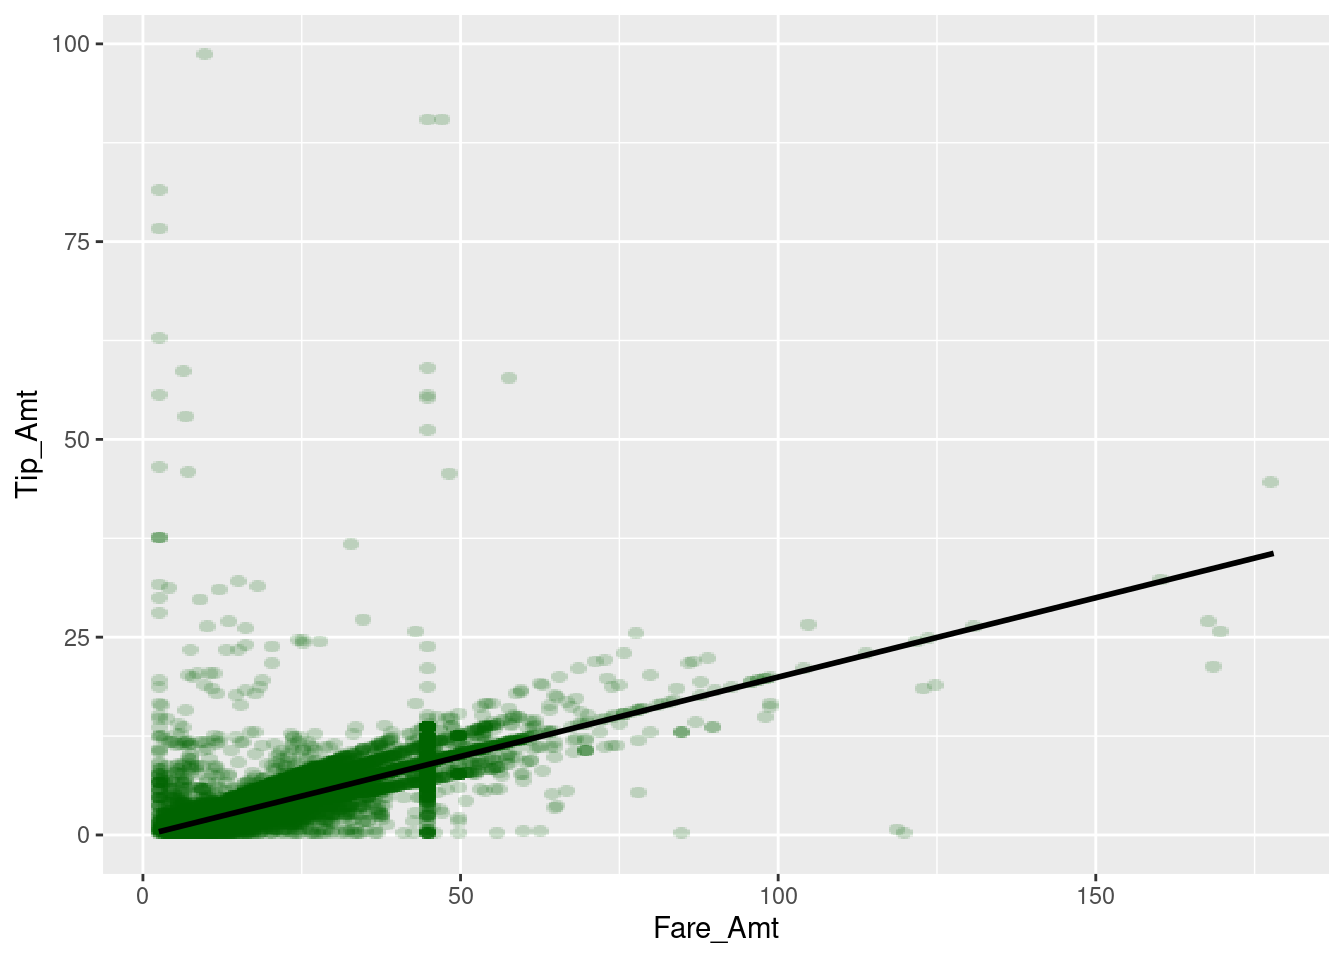
\includegraphics{bigdata_files/figure-latex/unnamed-chunk-198-1.pdf}

This practical approach does not require you to define every aspect of a theme. If you indeed want completely define every aspect of a theme, you can set \texttt{complete=TRUE} when calling the theme function.

\begin{Shaded}
\begin{Highlighting}[]
\CommentTok{\# \textquotesingle{}define\textquotesingle{} a new theme}
\NormalTok{my\_serif\_theme }\OtherTok{\textless{}{-}}      
  \FunctionTok{theme\_bw}\NormalTok{(}\AttributeTok{base\_size =} \DecValTok{18}\NormalTok{, }\AttributeTok{base\_family =} \StringTok{"serif"}\NormalTok{) }\SpecialCharTok{+}
  \FunctionTok{theme}\NormalTok{(}\AttributeTok{axis.title =} \FunctionTok{element\_text}\NormalTok{(}\AttributeTok{face=}\StringTok{"bold"}\NormalTok{), }\AttributeTok{complete =} \ConstantTok{TRUE}\NormalTok{)}

\CommentTok{\# apply it }
\NormalTok{modelplot }\SpecialCharTok{+}
     \FunctionTok{geom\_point}\NormalTok{(}\AttributeTok{alpha=}\FloatTok{0.2}\NormalTok{, }\AttributeTok{colour=}\StringTok{"darkgreen"}\NormalTok{) }\SpecialCharTok{+}
     \FunctionTok{geom\_smooth}\NormalTok{(}\AttributeTok{method =} \StringTok{"lm"}\NormalTok{, }\AttributeTok{colour =} \StringTok{"black"}\NormalTok{) }\SpecialCharTok{+}
     \FunctionTok{ylab}\NormalTok{(}\StringTok{"Amount of tip paid (in USD)"}\NormalTok{) }\SpecialCharTok{+}
     \FunctionTok{xlab}\NormalTok{(}\StringTok{"Amount of fare paid (in USD)"}\NormalTok{) }\SpecialCharTok{+}
\NormalTok{  theme\_my\_serif}
\end{Highlighting}
\end{Shaded}

\begin{verbatim}
## `geom_smooth()` using formula 'y ~ x'
\end{verbatim}

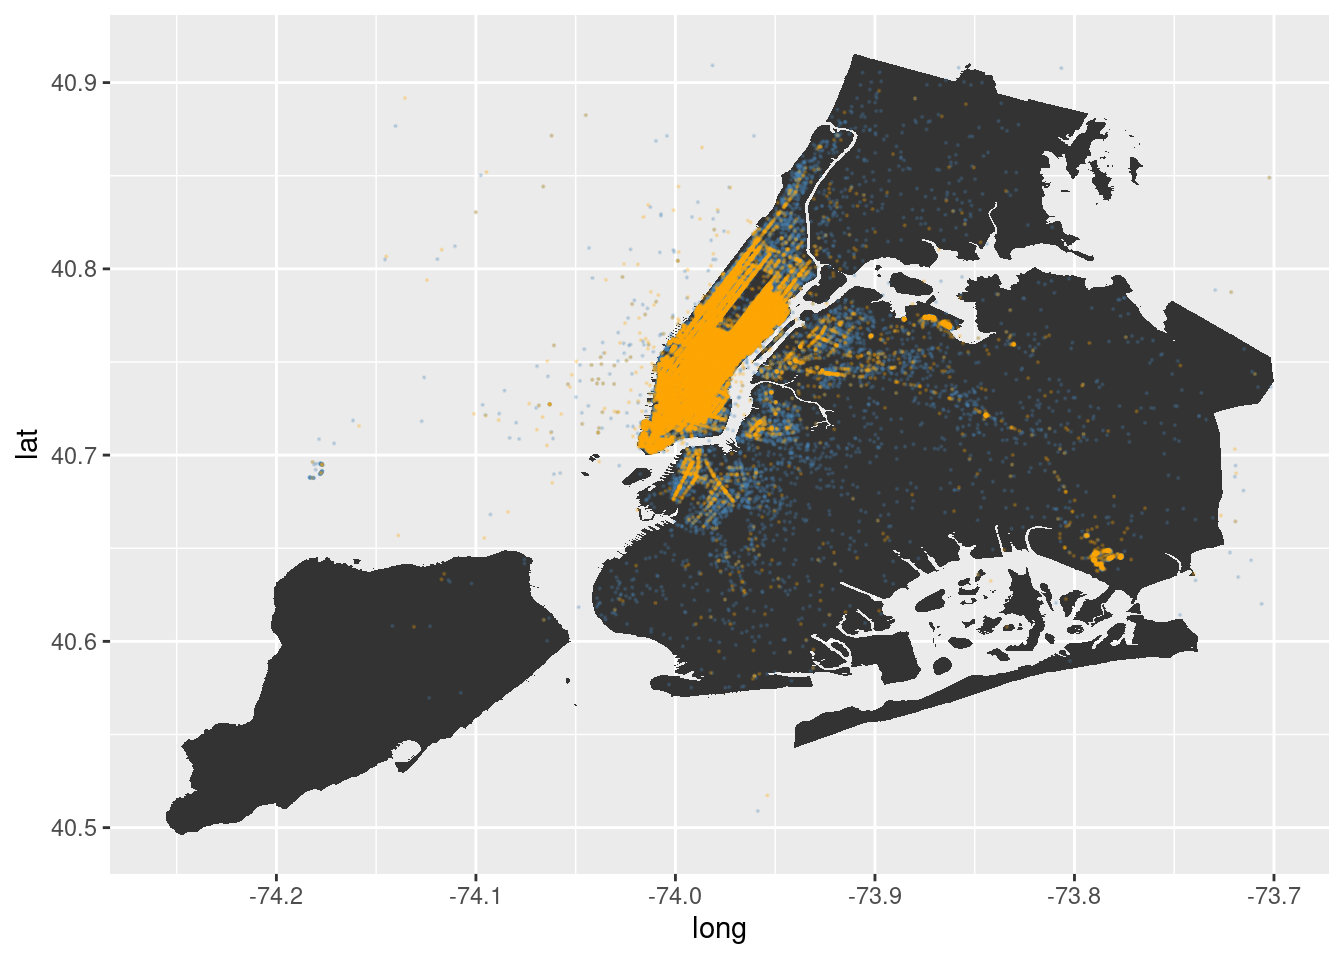
\includegraphics{bigdata_files/figure-latex/unnamed-chunk-199-1.pdf}

Note that since we have only defined one aspect (bold axis titles), the rest of the elements follow the default theme.

Importantly, the approach outlined above does technically not really create a new theme like \texttt{theme\_bw()}, as these pre-defined themes are implemented as functions. Note that we add the new theme simply with \texttt{+\ theme\_my\_serif} to the plot (no parentheses). In practice this is the most simple approach and it provides all the functionality you need in order to apply your own `theme' to each of your plots.

\hypertarget{implementing-actual-themes-as-functions.}{%
\subsection{Implementing actual themes as functions.}\label{implementing-actual-themes-as-functions.}}

If you really want to implement a theme as a function. The following blueprint can get you started.

\begin{Shaded}
\begin{Highlighting}[]
\CommentTok{\# define own theme}
\NormalTok{theme\_my\_serif }\OtherTok{\textless{}{-}} 
  \ControlFlowTok{function}\NormalTok{(}\AttributeTok{base\_size =} \DecValTok{15}\NormalTok{,}
           \AttributeTok{base\_family =} \StringTok{""}\NormalTok{,}
           \AttributeTok{base\_line\_size =}\NormalTok{ base\_size}\SpecialCharTok{/}\DecValTok{170}\NormalTok{,}
           \AttributeTok{base\_rect\_size =}\NormalTok{ base\_size}\SpecialCharTok{/}\DecValTok{170}\NormalTok{)\{ }
    
    \FunctionTok{theme\_bw}\NormalTok{(}\AttributeTok{base\_size =}\NormalTok{ base\_size,}
             \AttributeTok{base\_family =}\NormalTok{ base\_family,}
             \AttributeTok{base\_line\_size =}\NormalTok{ base\_size}\SpecialCharTok{/}\DecValTok{170}\NormalTok{,}
             \AttributeTok{base\_rect\_size =}\NormalTok{ base\_size}\SpecialCharTok{/}\DecValTok{170}\NormalTok{) }\SpecialCharTok{\%+replace\%}    \CommentTok{\# use theme\_bw() as a basis but replace some design elements}
    \FunctionTok{theme}\NormalTok{(}
      \AttributeTok{axis.title =} \FunctionTok{element\_text}\NormalTok{(}\AttributeTok{face=}\StringTok{"bold"}\NormalTok{)}
\NormalTok{    )}
\NormalTok{  \}}

\CommentTok{\# apply the theme}
\CommentTok{\# apply it }
\NormalTok{modelplot }\SpecialCharTok{+}
     \FunctionTok{geom\_point}\NormalTok{(}\AttributeTok{alpha=}\FloatTok{0.2}\NormalTok{, }\AttributeTok{colour=}\StringTok{"darkgreen"}\NormalTok{) }\SpecialCharTok{+}
     \FunctionTok{geom\_smooth}\NormalTok{(}\AttributeTok{method =} \StringTok{"lm"}\NormalTok{, }\AttributeTok{colour =} \StringTok{"black"}\NormalTok{) }\SpecialCharTok{+}
     \FunctionTok{ylab}\NormalTok{(}\StringTok{"Amount of tip paid (in USD)"}\NormalTok{) }\SpecialCharTok{+}
     \FunctionTok{xlab}\NormalTok{(}\StringTok{"Amount of fare paid (in USD)"}\NormalTok{) }\SpecialCharTok{+}
  \FunctionTok{theme\_my\_serif}\NormalTok{(}\AttributeTok{base\_size =} \DecValTok{18}\NormalTok{, }\AttributeTok{base\_family=}\StringTok{"serif"}\NormalTok{)}
\end{Highlighting}
\end{Shaded}

\begin{verbatim}
## `geom_smooth()` using formula 'y ~ x'
\end{verbatim}

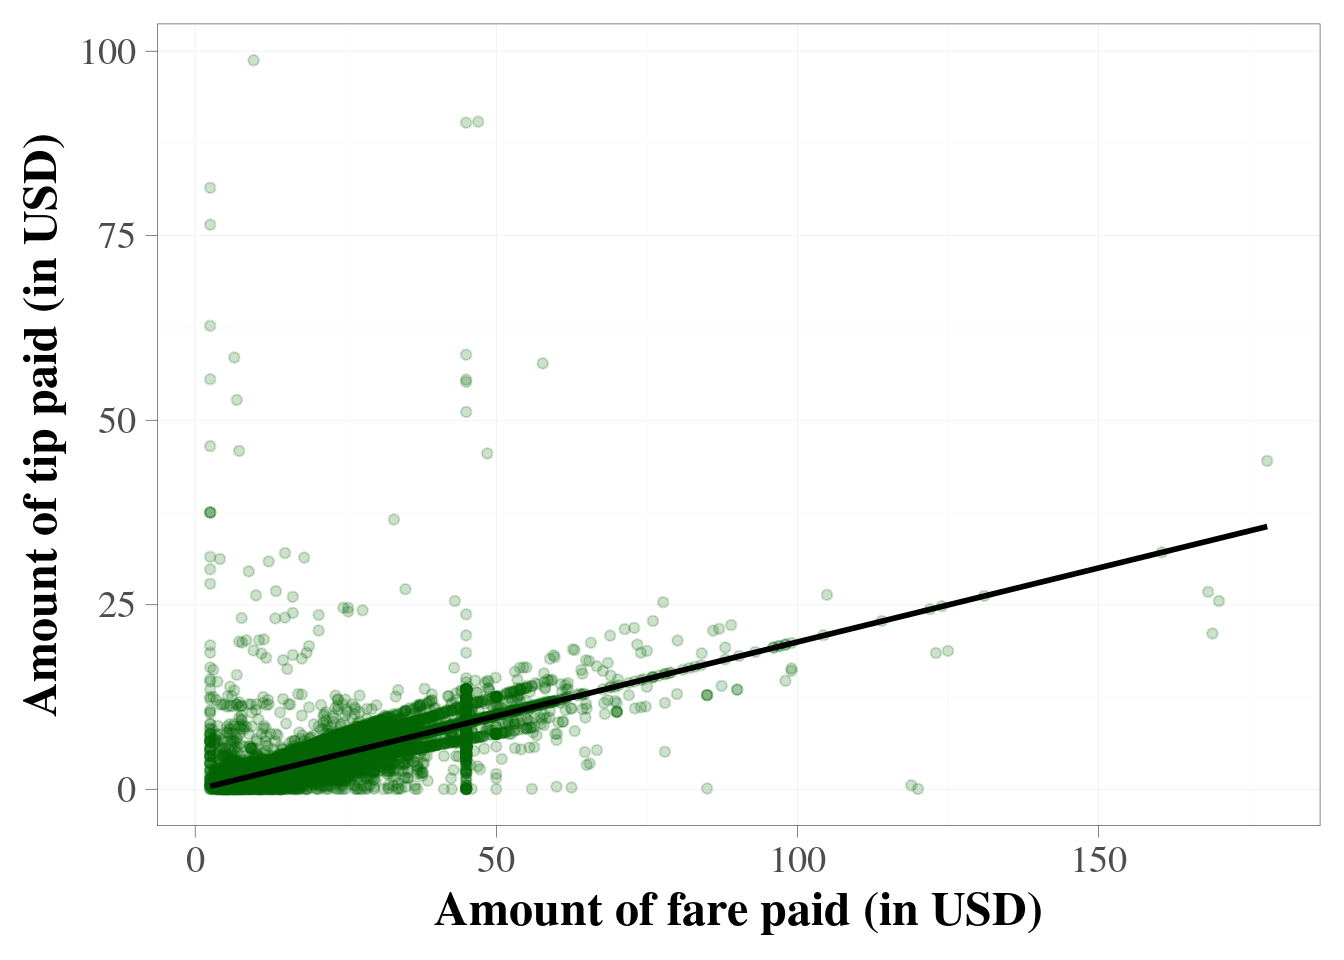
\includegraphics{bigdata_files/figure-latex/unnamed-chunk-200-1.pdf}

\hypertarget{visualize-time-and-space}{%
\section{Visualize Time and Space}\label{visualize-time-and-space}}

The previous visualization exercises were focused on visually exploring patterns in the tipping behavior of people taking a NYC yellow cap ride. Based on the same data set, will explore the time dimension and spatial dimension of the TLC Yellow Cap data. That is, we explore where trips tend to start and end, depending on the time of the day.

\hypertarget{preparations}{%
\subsection{Preparations}\label{preparations}}

For the visualization of spatial data we first load additional packages that give R some \href{https://en.wikipedia.org/wiki/Geographic_information_system}{GIS} features.

\begin{Shaded}
\begin{Highlighting}[]
\CommentTok{\# load GIS packages}
\FunctionTok{library}\NormalTok{(rgdal)}
\FunctionTok{library}\NormalTok{(rgeos)}
\end{Highlighting}
\end{Shaded}

Moreover, we download and import a so-called \href{https://en.wikipedia.org/wiki/Shapefile}{`shape file'} (a geospatial data format) of New York City. This will be the basis for our visualization of the spatial dimension of taxi trips. The file is downloaded from \href{https://www1.nyc.gov/site/planning/index.page}{New York's Department of City Planning} and indicates the city's community district borders.\footnote{Similar files are provided online by most city authorities in developed countries. See, for example, GIS Data for the City and Canton of Zurich: \url{https://maps.zh.ch/}.}

\begin{Shaded}
\begin{Highlighting}[]
\CommentTok{\# download the zipped shapefile to a temporary file, unzip}
\NormalTok{URL }\OtherTok{\textless{}{-}} \StringTok{"https://www1.nyc.gov/assets/planning/download/zip/data{-}maps/open{-}data/nycd\_19a.zip"}
\NormalTok{tmp\_file }\OtherTok{\textless{}{-}} \FunctionTok{tempfile}\NormalTok{()}
\FunctionTok{download.file}\NormalTok{(URL, tmp\_file)}
\NormalTok{file\_path }\OtherTok{\textless{}{-}} \FunctionTok{unzip}\NormalTok{(tmp\_file, }\AttributeTok{exdir=} \StringTok{"data"}\NormalTok{)}
\CommentTok{\# delete the temporary file}
\FunctionTok{unlink}\NormalTok{(tmp\_file)}
\end{Highlighting}
\end{Shaded}

Now we can import the shape file and have a look at how the GIS data is structured.

\begin{Shaded}
\begin{Highlighting}[]
\CommentTok{\# read GIS data}
\NormalTok{nyc\_map }\OtherTok{\textless{}{-}} \FunctionTok{readOGR}\NormalTok{(file\_path[}\DecValTok{1}\NormalTok{], }\AttributeTok{verbose =} \ConstantTok{FALSE}\NormalTok{)}

\CommentTok{\# have a look at the GIS data}
\FunctionTok{summary}\NormalTok{(nyc\_map)}
\end{Highlighting}
\end{Shaded}

\begin{verbatim}
## Object of class SpatialPolygonsDataFrame
## Coordinates:
##      min     max
## x 913175 1067383
## y 120122  272844
## Is projected: TRUE 
## proj4string :
## [+proj=lcc +lat_0=40.1666666666667 +lon_0=-74
## +lat_1=41.0333333333333 +lat_2=40.6666666666667
## +x_0=300000 +y_0=0 +datum=NAD83 +units=us-ft
## +no_defs]
## Data attributes:
##      BoroCD      Shape_Leng       Shape_Area      
##  Min.   :101   Min.   : 23963   Min.   :2.43e+07  
##  1st Qu.:206   1st Qu.: 36611   1st Qu.:4.84e+07  
##  Median :308   Median : 52246   Median :8.27e+07  
##  Mean   :297   Mean   : 74890   Mean   :1.19e+08  
##  3rd Qu.:406   3rd Qu.: 85711   3rd Qu.:1.37e+08  
##  Max.   :595   Max.   :270660   Max.   :5.99e+08
\end{verbatim}

Note that the coordinates are not in the usual longitude and latitude units. The original map uses a different projection than the TLC data of cap trips records. Before plotting, we thus have to change the projection to be in line with the TLC data.

\begin{Shaded}
\begin{Highlighting}[]
\CommentTok{\# transform the projection}
\NormalTok{nyc\_map }\OtherTok{\textless{}{-}} \FunctionTok{spTransform}\NormalTok{(nyc\_map, }\FunctionTok{CRS}\NormalTok{(}\StringTok{"+proj=longlat +datum=WGS84 +no\_defs +ellps=WGS84 +towgs84=0,0,0"}\NormalTok{))}
\CommentTok{\# check result}
\FunctionTok{summary}\NormalTok{(nyc\_map)}
\end{Highlighting}
\end{Shaded}

\begin{verbatim}
## Object of class SpatialPolygonsDataFrame
## Coordinates:
##      min    max
## x -74.26 -73.70
## y  40.50  40.92
## Is projected: FALSE 
## proj4string : [+proj=longlat +datum=WGS84 +no_defs]
## Data attributes:
##      BoroCD      Shape_Leng       Shape_Area      
##  Min.   :101   Min.   : 23963   Min.   :2.43e+07  
##  1st Qu.:206   1st Qu.: 36611   1st Qu.:4.84e+07  
##  Median :308   Median : 52246   Median :8.27e+07  
##  Mean   :297   Mean   : 74890   Mean   :1.19e+08  
##  3rd Qu.:406   3rd Qu.: 85711   3rd Qu.:1.37e+08  
##  Max.   :595   Max.   :270660   Max.   :5.99e+08
\end{verbatim}

One last preparatory step is to convert the map data to a \texttt{data.frame} for plotting with \texttt{ggplot}.

\begin{Shaded}
\begin{Highlighting}[]
\NormalTok{nyc\_map }\OtherTok{\textless{}{-}} \FunctionTok{fortify}\NormalTok{(nyc\_map)}
\end{Highlighting}
\end{Shaded}

\hypertarget{pick-up-and-drop-off-locations}{%
\subsection{Pick-up and drop-off locations}\label{pick-up-and-drop-off-locations}}

Since trips might actually start or end outside of NYC, we first restrict the sample of trips to those within the boundary box of the map. For the sake of the exercise, we only select a random sample of \texttt{50000} trips from the remaining trip records.

\begin{Shaded}
\begin{Highlighting}[]
\CommentTok{\# taxi trips plot data}
\NormalTok{taxi\_trips }\OtherTok{\textless{}{-}}\NormalTok{ taxi[start\_long }\SpecialCharTok{\textless{}=} \FunctionTok{max}\NormalTok{(nyc\_map}\SpecialCharTok{$}\NormalTok{long) }\SpecialCharTok{\&} 
\NormalTok{                        start\_long }\SpecialCharTok{\textgreater{}=} \FunctionTok{min}\NormalTok{(nyc\_map}\SpecialCharTok{$}\NormalTok{long) }\SpecialCharTok{\&}
\NormalTok{                        dest\_long }\SpecialCharTok{\textless{}=} \FunctionTok{max}\NormalTok{(nyc\_map}\SpecialCharTok{$}\NormalTok{long) }\SpecialCharTok{\&}
\NormalTok{                        dest\_long }\SpecialCharTok{\textgreater{}=} \FunctionTok{min}\NormalTok{(nyc\_map}\SpecialCharTok{$}\NormalTok{long) }\SpecialCharTok{\&}
\NormalTok{                        start\_lat }\SpecialCharTok{\textless{}=} \FunctionTok{max}\NormalTok{(nyc\_map}\SpecialCharTok{$}\NormalTok{lat) }\SpecialCharTok{\&} 
\NormalTok{                        start\_lat }\SpecialCharTok{\textgreater{}=} \FunctionTok{min}\NormalTok{(nyc\_map}\SpecialCharTok{$}\NormalTok{lat) }\SpecialCharTok{\&}
\NormalTok{                        dest\_lat }\SpecialCharTok{\textless{}=} \FunctionTok{max}\NormalTok{(nyc\_map}\SpecialCharTok{$}\NormalTok{lat) }\SpecialCharTok{\&}
\NormalTok{                        dest\_lat }\SpecialCharTok{\textgreater{}=} \FunctionTok{min}\NormalTok{(nyc\_map}\SpecialCharTok{$}\NormalTok{lat) }
\NormalTok{                        ]}
\NormalTok{taxi\_trips }\OtherTok{\textless{}{-}}\NormalTok{ taxi\_trips[base}\SpecialCharTok{::}\FunctionTok{sample}\NormalTok{(}\DecValTok{1}\SpecialCharTok{:}\FunctionTok{nrow}\NormalTok{(taxi\_trips), }\DecValTok{50000}\NormalTok{)]}
\end{Highlighting}
\end{Shaded}

In order to visualize how the cap traffic is changing over the course of the day, we add an additional variable called \texttt{start\_time} in which we store the time (hour) of the day a trip started.

\begin{Shaded}
\begin{Highlighting}[]
\NormalTok{taxi\_trips}\SpecialCharTok{$}\NormalTok{start\_time }\OtherTok{\textless{}{-}} \FunctionTok{hour}\NormalTok{(taxi\_trips}\SpecialCharTok{$}\NormalTok{pickup\_time)}
\end{Highlighting}
\end{Shaded}

Particularly, we want to look at differences between, morning, afternoon, and evening/night.

\begin{Shaded}
\begin{Highlighting}[]
\CommentTok{\# define new variable for facets}
\NormalTok{taxi\_trips}\SpecialCharTok{$}\NormalTok{time\_of\_day }\OtherTok{\textless{}{-}} \StringTok{"Morning"}
\NormalTok{taxi\_trips[start\_time }\SpecialCharTok{\textgreater{}} \DecValTok{12} \SpecialCharTok{\&}\NormalTok{ start\_time }\SpecialCharTok{\textless{}} \DecValTok{17}\NormalTok{]}\SpecialCharTok{$}\NormalTok{time\_of\_day }\OtherTok{\textless{}{-}} \StringTok{"Afternoon"}
\NormalTok{taxi\_trips[start\_time }\SpecialCharTok{\%in\%} \FunctionTok{c}\NormalTok{(}\DecValTok{17}\SpecialCharTok{:}\DecValTok{24}\NormalTok{, }\DecValTok{0}\SpecialCharTok{:}\DecValTok{5}\NormalTok{)]}\SpecialCharTok{$}\NormalTok{time\_of\_day }\OtherTok{\textless{}{-}} \StringTok{"Evening/Night"}
\NormalTok{taxi\_trips}\SpecialCharTok{$}\NormalTok{time\_of\_day  }\OtherTok{\textless{}{-}} \FunctionTok{factor}\NormalTok{(taxi\_trips}\SpecialCharTok{$}\NormalTok{time\_of\_day, }\AttributeTok{levels =} \FunctionTok{c}\NormalTok{(}\StringTok{"Morning"}\NormalTok{, }\StringTok{"Afternoon"}\NormalTok{, }\StringTok{"Evening/Night"}\NormalTok{))}
\end{Highlighting}
\end{Shaded}

We initiate the plot by first setting up the canvas with our taxi trips data. Then, we add the map as a first layer.

\begin{Shaded}
\begin{Highlighting}[]
\CommentTok{\# set up the canvas}
\NormalTok{locations }\OtherTok{\textless{}{-}} \FunctionTok{ggplot}\NormalTok{(taxi\_trips, }\FunctionTok{aes}\NormalTok{(}\AttributeTok{x=}\NormalTok{long, }\AttributeTok{y=}\NormalTok{lat))}
\CommentTok{\# add the map geometry}
\NormalTok{locations }\OtherTok{\textless{}{-}}\NormalTok{ locations }\SpecialCharTok{+} \FunctionTok{geom\_map}\NormalTok{(}\AttributeTok{data =}\NormalTok{ nyc\_map,}
                                  \AttributeTok{map =}\NormalTok{ nyc\_map,}
                                  \FunctionTok{aes}\NormalTok{(}\AttributeTok{map\_id =}\NormalTok{ id))}
\NormalTok{locations}
\end{Highlighting}
\end{Shaded}

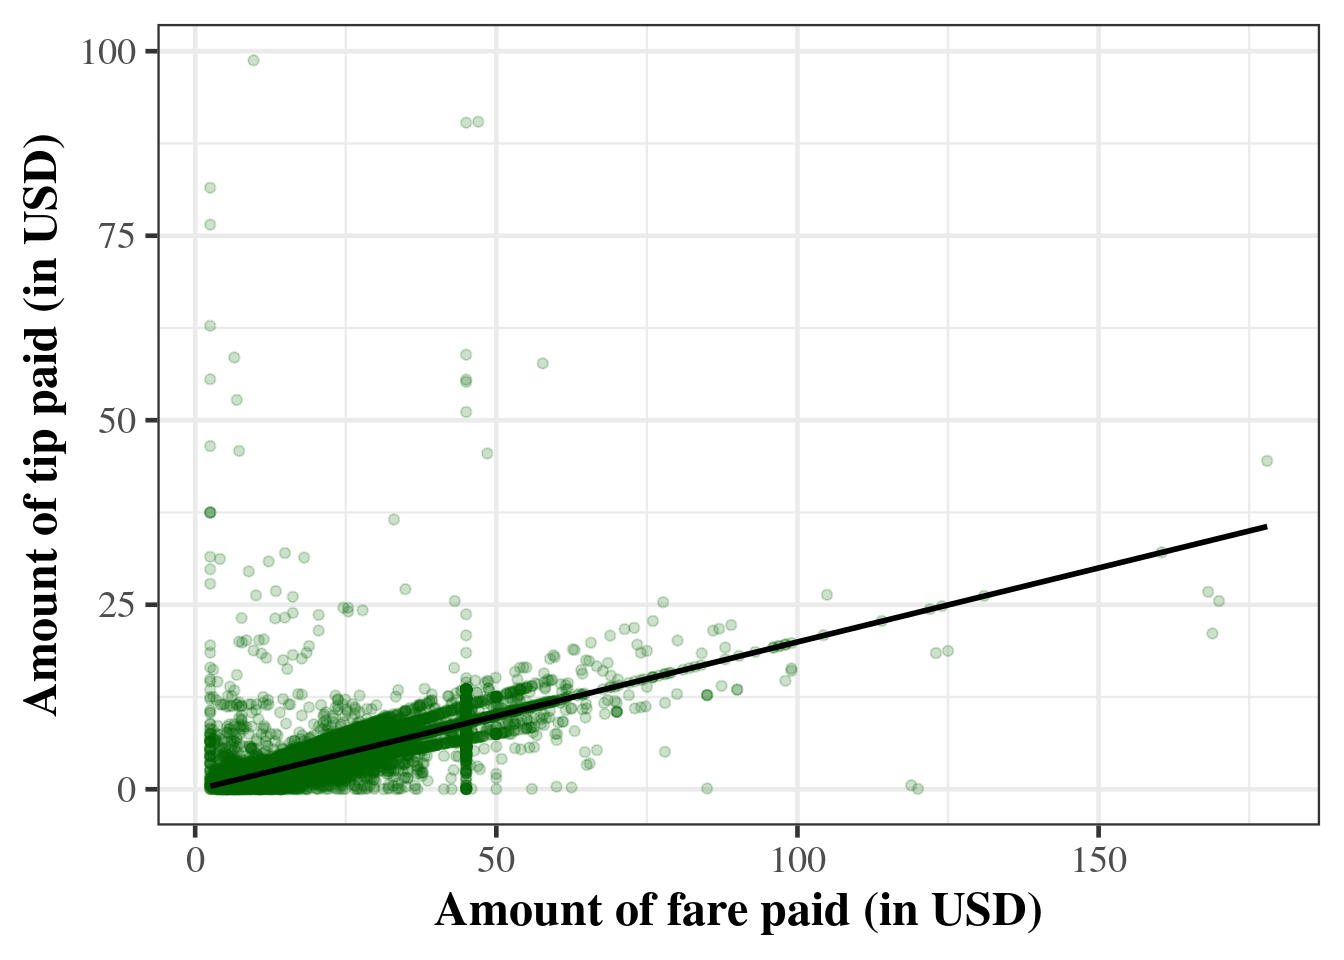
\includegraphics{bigdata_files/figure-latex/unnamed-chunk-209-1.pdf}

Now we can start adding the pick-up and drop-off locations of cap trips.

\begin{Shaded}
\begin{Highlighting}[]
\CommentTok{\# add pick{-}up locations to plot}
\NormalTok{locations }\SpecialCharTok{+} 
     \FunctionTok{geom\_point}\NormalTok{(}\FunctionTok{aes}\NormalTok{(}\AttributeTok{x=}\NormalTok{start\_long, }\AttributeTok{y=}\NormalTok{start\_lat),}
                \AttributeTok{color=}\StringTok{"orange"}\NormalTok{,}
                \AttributeTok{size =} \FloatTok{0.1}\NormalTok{,}
                \AttributeTok{alpha =} \FloatTok{0.2}\NormalTok{)}
\end{Highlighting}
\end{Shaded}

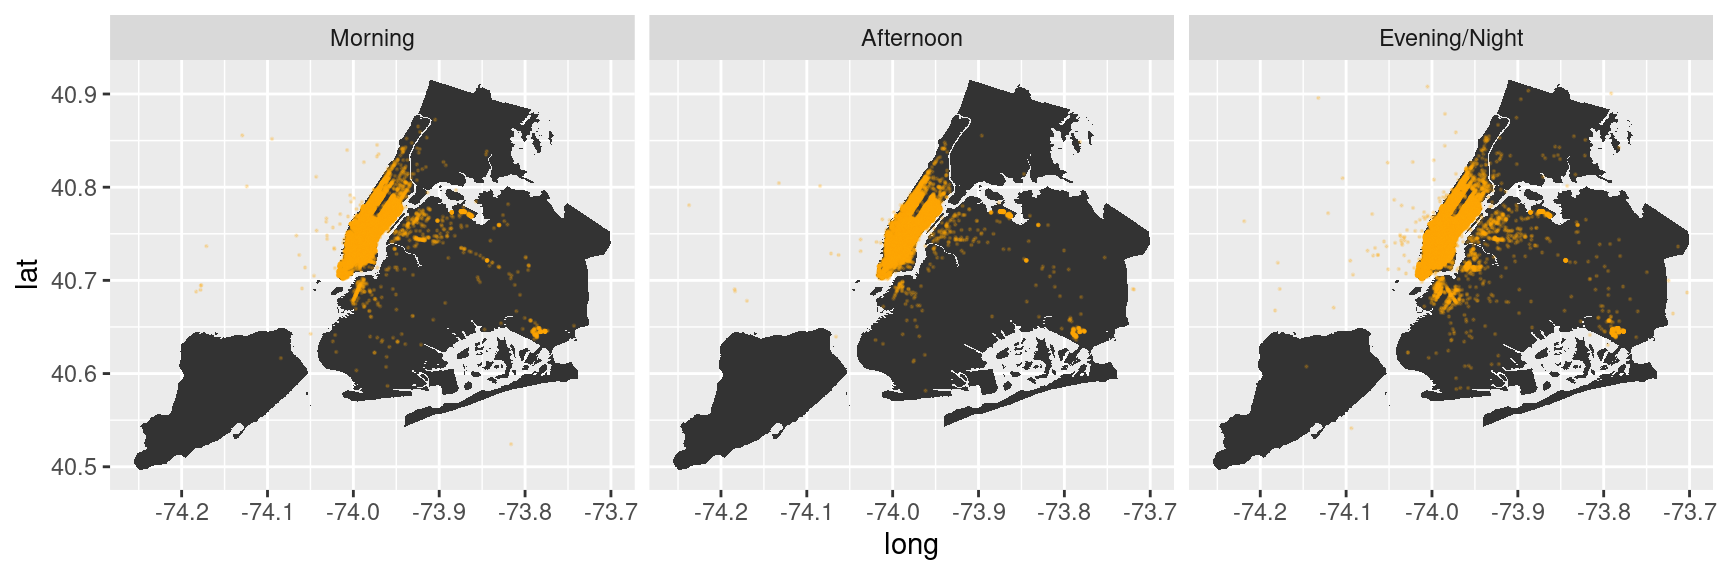
\includegraphics{bigdata_files/figure-latex/unnamed-chunk-210-1.pdf}

As to be expected, most of the trips start in Manhattan. Now let's look at where trips end.

\begin{Shaded}
\begin{Highlighting}[]
\CommentTok{\# add pick{-}up locations to plot}
\NormalTok{locations }\SpecialCharTok{+}
     \FunctionTok{geom\_point}\NormalTok{(}\FunctionTok{aes}\NormalTok{(}\AttributeTok{x=}\NormalTok{dest\_long, }\AttributeTok{y=}\NormalTok{dest\_lat),}
                \AttributeTok{color=}\StringTok{"steelblue"}\NormalTok{,}
                \AttributeTok{size =} \FloatTok{0.1}\NormalTok{,}
                \AttributeTok{alpha =} \FloatTok{0.2}\NormalTok{) }\SpecialCharTok{+}
     \FunctionTok{geom\_point}\NormalTok{(}\FunctionTok{aes}\NormalTok{(}\AttributeTok{x=}\NormalTok{start\_long, }\AttributeTok{y=}\NormalTok{start\_lat),}
                \AttributeTok{color=}\StringTok{"orange"}\NormalTok{,}
                \AttributeTok{size =} \FloatTok{0.1}\NormalTok{,}
                \AttributeTok{alpha =} \FloatTok{0.2}\NormalTok{)}
\end{Highlighting}
\end{Shaded}

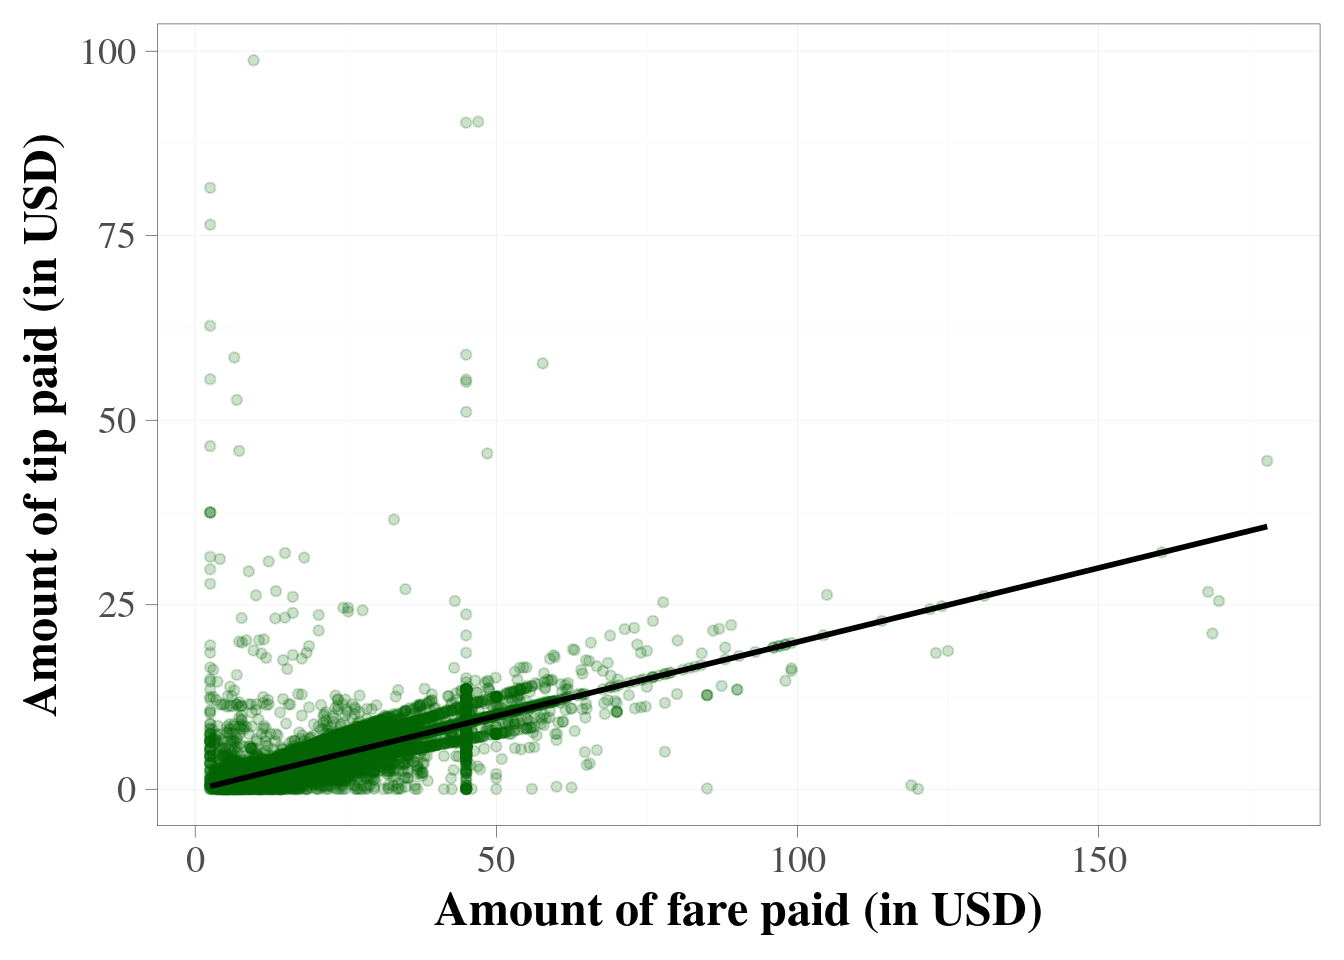
\includegraphics{bigdata_files/figure-latex/unnamed-chunk-211-1.pdf}

Incidentally, more trips tend to end outside of Manhattan. And the destinations seem to be broader spread across the city then the pick-up locations. Most destinations are still in Manhattan, though.

Now let's have a look at how this picture changes depending on the time of the day.

\begin{Shaded}
\begin{Highlighting}[]
\CommentTok{\# pick{-}up locations }
\NormalTok{locations }\SpecialCharTok{+}
     \FunctionTok{geom\_point}\NormalTok{(}\FunctionTok{aes}\NormalTok{(}\AttributeTok{x=}\NormalTok{start\_long, }\AttributeTok{y=}\NormalTok{start\_lat),}
                \AttributeTok{color=}\StringTok{"orange"}\NormalTok{,}
                \AttributeTok{size =} \FloatTok{0.1}\NormalTok{,}
                \AttributeTok{alpha =} \FloatTok{0.2}\NormalTok{) }\SpecialCharTok{+}
     \FunctionTok{facet\_wrap}\NormalTok{(}\FunctionTok{vars}\NormalTok{(time\_of\_day))}
\end{Highlighting}
\end{Shaded}

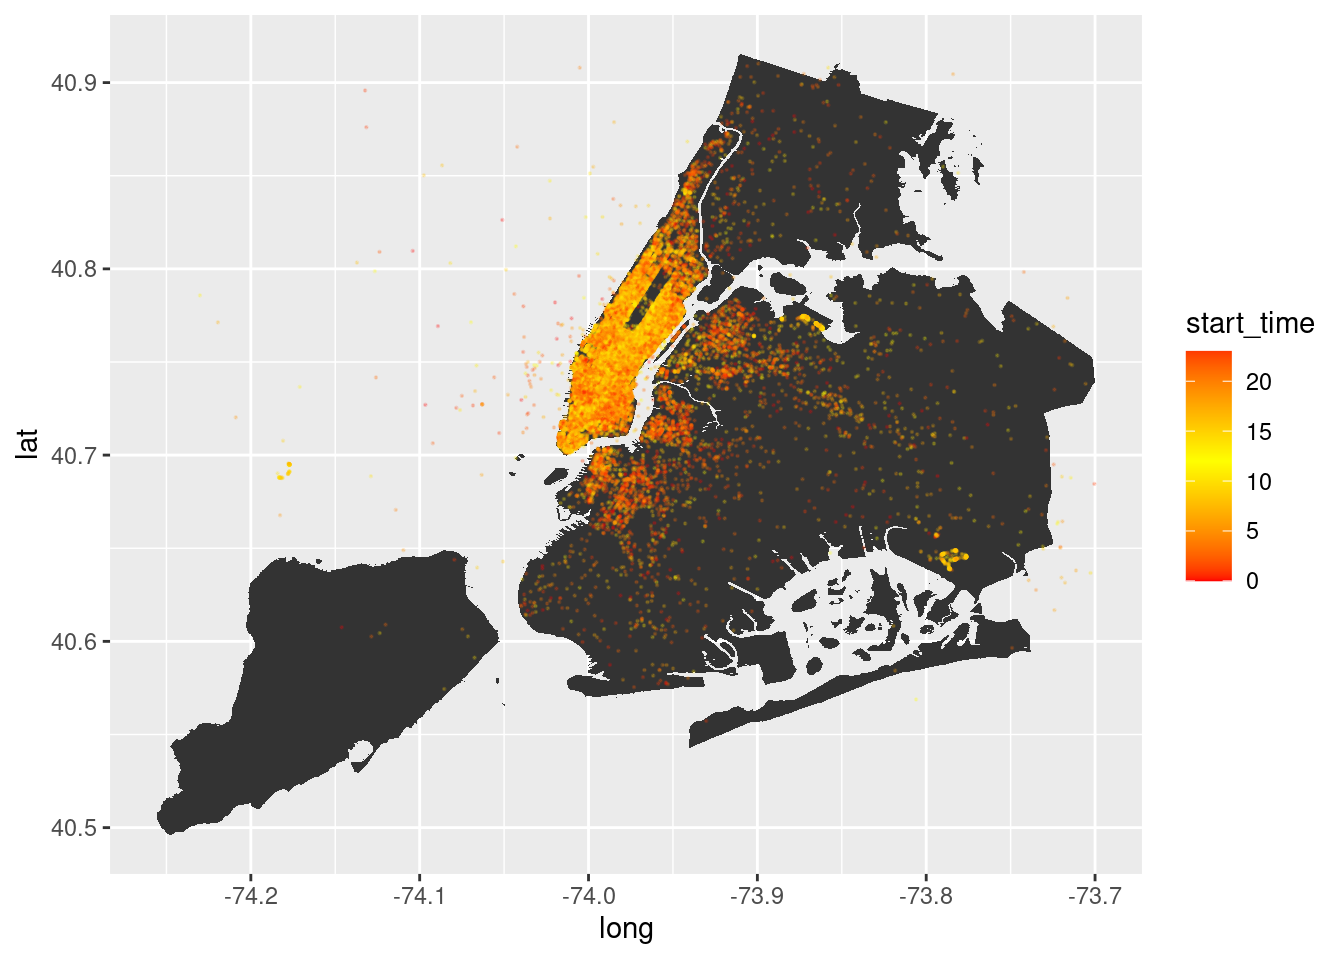
\includegraphics{bigdata_files/figure-latex/unnamed-chunk-212-1.pdf}

\begin{Shaded}
\begin{Highlighting}[]
\CommentTok{\# drop{-}off locations }
\NormalTok{locations }\SpecialCharTok{+}
     \FunctionTok{geom\_point}\NormalTok{(}\FunctionTok{aes}\NormalTok{(}\AttributeTok{x=}\NormalTok{dest\_long, }\AttributeTok{y=}\NormalTok{dest\_lat),}
                \AttributeTok{color=}\StringTok{"steelblue"}\NormalTok{,}
                \AttributeTok{size =} \FloatTok{0.1}\NormalTok{,}
                \AttributeTok{alpha =} \FloatTok{0.2}\NormalTok{) }\SpecialCharTok{+}
     \FunctionTok{facet\_wrap}\NormalTok{(}\FunctionTok{vars}\NormalTok{(time\_of\_day))}
\end{Highlighting}
\end{Shaded}

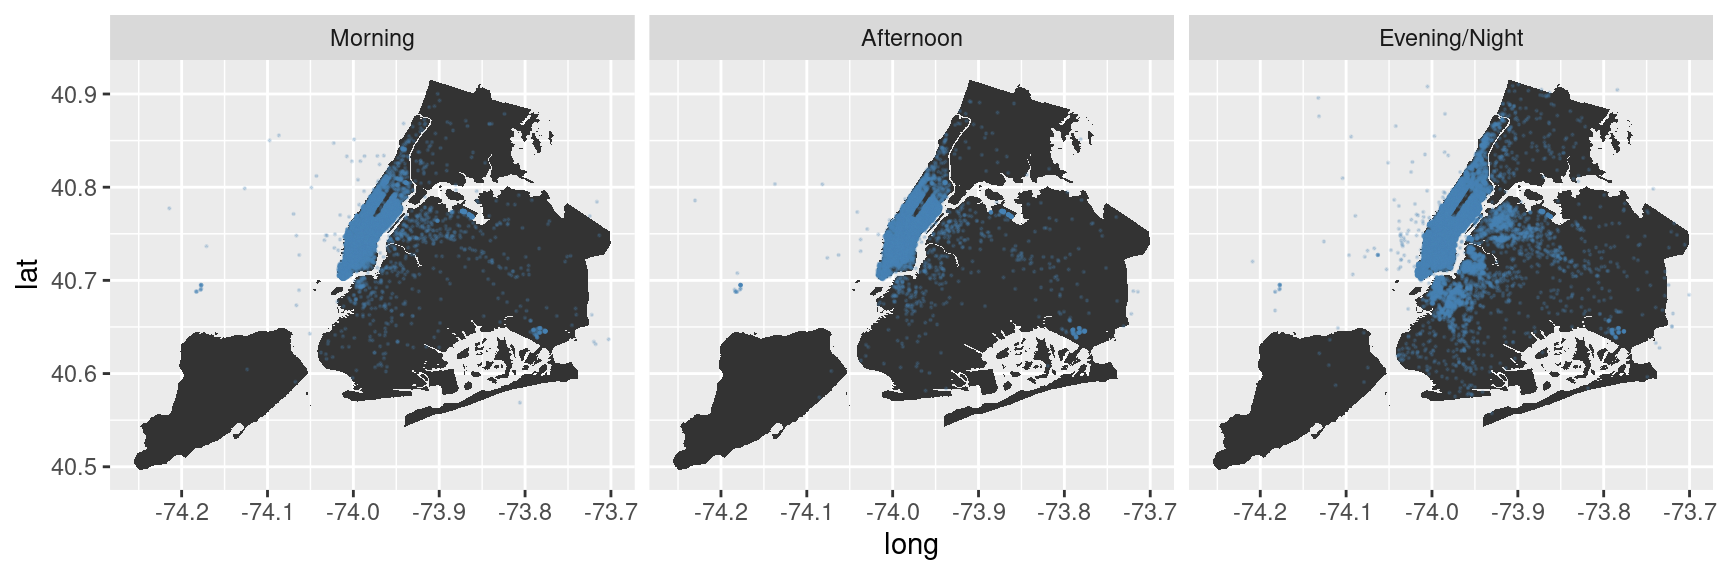
\includegraphics{bigdata_files/figure-latex/unnamed-chunk-213-1.pdf}

Alternatively, we can plot the hours on a continuous scale.

\begin{Shaded}
\begin{Highlighting}[]
\CommentTok{\# drop{-}off locations }
\NormalTok{locations }\SpecialCharTok{+}
     \FunctionTok{geom\_point}\NormalTok{(}\FunctionTok{aes}\NormalTok{(}\AttributeTok{x=}\NormalTok{dest\_long, }\AttributeTok{y=}\NormalTok{dest\_lat, }\AttributeTok{color =}\NormalTok{ start\_time ),}
                \AttributeTok{size =} \FloatTok{0.1}\NormalTok{,}
                \AttributeTok{alpha =} \FloatTok{0.2}\NormalTok{) }\SpecialCharTok{+}
     \FunctionTok{scale\_colour\_gradient2}\NormalTok{( }\AttributeTok{low =} \StringTok{"red"}\NormalTok{, }\AttributeTok{mid =} \StringTok{"yellow"}\NormalTok{, }\AttributeTok{high =} \StringTok{"red"}\NormalTok{,}
                             \AttributeTok{midpoint =} \DecValTok{12}\NormalTok{)}
\end{Highlighting}
\end{Shaded}

\includegraphics{bigdata_files/figure-latex/unnamed-chunk-214-1.pdf}

\hypertarget{excursus-change-color-schemes}{%
\section{Excursus: change color schemes}\label{excursus-change-color-schemes}}

In the example above we use \texttt{scale\_colour\_gradient2()} to modify the color gradient used to visualize the start time of taxi trips. By default, ggplot would plot the following (default gradient color setting):

\begin{Shaded}
\begin{Highlighting}[]
\CommentTok{\# drop{-}off locations }
\NormalTok{locations }\SpecialCharTok{+}
     \FunctionTok{geom\_point}\NormalTok{(}\FunctionTok{aes}\NormalTok{(}\AttributeTok{x=}\NormalTok{dest\_long, }\AttributeTok{y=}\NormalTok{dest\_lat, }\AttributeTok{color =}\NormalTok{ start\_time ),}
                \AttributeTok{size =} \FloatTok{0.1}\NormalTok{,}
                \AttributeTok{alpha =} \FloatTok{0.2}\NormalTok{) }
\end{Highlighting}
\end{Shaded}

\includegraphics{bigdata_files/figure-latex/unnamed-chunk-215-1.pdf}

\texttt{ggplot2} offers various functions to modify the color scales used in a plot. In the case of the example above, we visualize values of a continuous variable. Hence we use a gradient color scale. In case of categorical variables we need to modify the default discrete color scale.

Recall the plot illustrating tipping behavior, where we highlight in which observations the client payd with credit card, cash, etc.

\begin{Shaded}
\begin{Highlighting}[]
\CommentTok{\# indicate natural numbers}
\NormalTok{taxi[, dollar\_paid }\SpecialCharTok{:}\ErrorTok{=} \FunctionTok{ifelse}\NormalTok{(tip\_amount }\SpecialCharTok{==} \FunctionTok{round}\NormalTok{(tip\_amount,}\DecValTok{0}\NormalTok{), }\StringTok{"Full"}\NormalTok{, }\StringTok{"Fraction"}\NormalTok{),]}


\CommentTok{\# extended x/y plot}
\NormalTok{taxiplot }\SpecialCharTok{+}
     \FunctionTok{geom\_point}\NormalTok{(}\AttributeTok{alpha=}\FloatTok{0.2}\NormalTok{, }\FunctionTok{aes}\NormalTok{(}\AttributeTok{color=}\NormalTok{payment\_type)) }\SpecialCharTok{+}
     \FunctionTok{facet\_wrap}\NormalTok{(}\StringTok{"dollar\_paid"}\NormalTok{)}
\end{Highlighting}
\end{Shaded}

\includegraphics{bigdata_files/figure-latex/unnamed-chunk-216-1.pdf}

Since we do not further specify the discrete color scheme to be used, ggplot simply uses its default color scheme for this plot. We can change this as follows.

\begin{Shaded}
\begin{Highlighting}[]
\CommentTok{\# indicate natural numbers}
\NormalTok{taxi[, dollar\_paid }\SpecialCharTok{:}\ErrorTok{=} \FunctionTok{ifelse}\NormalTok{(tip\_amount }\SpecialCharTok{==} \FunctionTok{round}\NormalTok{(tip\_amount,}\DecValTok{0}\NormalTok{), }\StringTok{"Full"}\NormalTok{, }\StringTok{"Fraction"}\NormalTok{),]}


\CommentTok{\# extended x/y plot}
\NormalTok{taxiplot }\SpecialCharTok{+}
     \FunctionTok{geom\_point}\NormalTok{(}\AttributeTok{alpha=}\FloatTok{0.2}\NormalTok{, }\FunctionTok{aes}\NormalTok{(}\AttributeTok{color=}\NormalTok{payment\_type)) }\SpecialCharTok{+}
     \FunctionTok{facet\_wrap}\NormalTok{(}\StringTok{"dollar\_paid"}\NormalTok{) }\SpecialCharTok{+}
     \FunctionTok{scale\_color\_discrete}\NormalTok{(}\AttributeTok{type =} \FunctionTok{c}\NormalTok{(}\StringTok{"red"}\NormalTok{, }\StringTok{"steelblue"}\NormalTok{, }\StringTok{"orange"}\NormalTok{, }\StringTok{"purple"}\NormalTok{))}
\end{Highlighting}
\end{Shaded}

\includegraphics{bigdata_files/figure-latex/unnamed-chunk-217-1.pdf}

\hypertarget{bottle-necks-in-local-big-data-analytics}{%
\chapter{Bottle Necks in Local Big Data Analytics}\label{bottle-necks-in-local-big-data-analytics}}

\hypertarget{case-study-data-import-and-memory-allocation}{%
\section{Case study: Data Import and Memory Allocation}\label{case-study-data-import-and-memory-allocation}}

Consider the first steps of a data pipeline in R. The first part of our script to import and clean the data looks as follows.

\begin{Shaded}
\begin{Highlighting}[]
\DocumentationTok{\#\#\#\#\#\#\#\#\#\#\#\#\#\#\#\#\#\#\#\#\#\#\#\#\#\#\#\#\#\#\#\#\#\#\#\#\#\#\#\#\#\#\#\#\#\#\#\#\#\#\#\#\#\#\#\#\#\#\#}
\CommentTok{\# Big Data Statistics: Flights data import and preparation}
\CommentTok{\#}
\CommentTok{\# U. Matter, January 2019}
\DocumentationTok{\#\#\#\#\#\#\#\#\#\#\#\#\#\#\#\#\#\#\#\#\#\#\#\#\#\#\#\#\#\#\#\#\#\#\#\#\#\#\#\#\#\#\#\#\#\#\#\#\#\#\#\#\#\#\#\#\#\#\#}

\CommentTok{\# SET UP {-}{-}{-}{-}{-}{-}{-}{-}{-}{-}{-}{-}{-}{-}{-}{-}{-}}

\CommentTok{\# fix variables}
\NormalTok{DATA\_PATH }\OtherTok{\textless{}{-}} \StringTok{"data/flights.csv"}

\CommentTok{\# DATA IMPORT {-}{-}{-}{-}{-}{-}{-}{-}{-}{-}{-}{-}{-}{-}{-}{-}}
\NormalTok{flights }\OtherTok{\textless{}{-}} \FunctionTok{read.csv}\NormalTok{(DATA\_PATH)}

\CommentTok{\# DATA PREPARATION {-}{-}{-}{-}{-}{-}{-}{-}}
\NormalTok{flights }\OtherTok{\textless{}{-}}\NormalTok{ flights[,}\SpecialCharTok{{-}}\DecValTok{1}\SpecialCharTok{:{-}}\DecValTok{3}\NormalTok{]}
\end{Highlighting}
\end{Shaded}

When running this script, we notice that some of the steps need a certain amount of time to process. Moreover, while none of these steps obviously involves a lot of computation (such as a matrix inversion or numerical optimization), it quite likely involves memory allocation. We first read data into RAM (allocated to R by our operating system). It turns out that there are different ways to allocate RAM when reading data from a CSV file. Depending on the amount of data to be read in, one or the other approach might be faster. We first investigate the RAM allocation in R with \texttt{mem\_change()} and \texttt{mem\_used()}.

\begin{Shaded}
\begin{Highlighting}[]
\CommentTok{\# SET UP {-}{-}{-}{-}{-}{-}{-}{-}{-}{-}{-}{-}{-}{-}{-}{-}{-}}

\CommentTok{\# fix variables}
\NormalTok{DATA\_PATH }\OtherTok{\textless{}{-}} \StringTok{"data/flights.csv"}
\CommentTok{\# load packages}
\FunctionTok{library}\NormalTok{(pryr) }


\CommentTok{\# check how much memory is used by R (overall)}
\FunctionTok{mem\_used}\NormalTok{()}
\end{Highlighting}
\end{Shaded}

\begin{verbatim}
## 2.31 GB
\end{verbatim}

\begin{Shaded}
\begin{Highlighting}[]
\CommentTok{\# check the change in memory due to each step}

\CommentTok{\# DATA IMPORT {-}{-}{-}{-}{-}{-}{-}{-}{-}{-}{-}{-}{-}{-}{-}{-}}
\FunctionTok{mem\_change}\NormalTok{(flights }\OtherTok{\textless{}{-}} \FunctionTok{read.csv}\NormalTok{(DATA\_PATH))}
\end{Highlighting}
\end{Shaded}

\begin{verbatim}
## 33 MB
\end{verbatim}

\begin{Shaded}
\begin{Highlighting}[]
\CommentTok{\# DATA PREPARATION {-}{-}{-}{-}{-}{-}{-}{-}}
\NormalTok{flights }\OtherTok{\textless{}{-}}\NormalTok{ flights[,}\SpecialCharTok{{-}}\DecValTok{1}\SpecialCharTok{:{-}}\DecValTok{3}\NormalTok{]}

\CommentTok{\# check how much memory is used by R now}
\FunctionTok{mem\_used}\NormalTok{()}
\end{Highlighting}
\end{Shaded}

\begin{verbatim}
## 2.34 GB
\end{verbatim}

The last result is kind of interesting. The object \texttt{flights} must have been larger right after importing it than at the end of the script. We have thrown out several variables, after all. Why does R still use that much memory? R does by default not `clean up' memory unless it is really necessary (meaning no more memory is available). In this case, R has still way more memory available from the operating system, thus there is no need to `collect the garbage' yet. However, we can force R to collect the garbage on the spot with \texttt{gc()}. This can be helpful to better keep track of the memory needed by an analytics script.

\begin{Shaded}
\begin{Highlighting}[]
\FunctionTok{gc}\NormalTok{()}
\end{Highlighting}
\end{Shaded}

\begin{verbatim}
##             used   (Mb) gc trigger (Mb)  max used
## Ncells   8529715  455.6   14810401  791  12986236
## Vcells 232255241 1772.0  409858047 3127 409846454
##          (Mb)
## Ncells  693.6
## Vcells 3126.9
\end{verbatim}

Now, let's see how we can improve the performance of this script with regard to memory allocation. Most memory is allocated when importing the file. Obviously, any improvement of the script must still result in importing all the data. However, there are different ways to read data into RAM. \texttt{read.csv()} reads all lines of a csv file consecutively. In contrast, \texttt{data.table::fread()} first `maps' the data file into memory and only then actually reads it in line by line. This involves an additional initial step, but the larger the file, the less relevant is this first step with regard to the total time needed to read all the data into memory. By switching on the \texttt{verbose} option, we can actually see what \texttt{fread} is doing.

\begin{Shaded}
\begin{Highlighting}[]
\CommentTok{\# load packages}
\FunctionTok{library}\NormalTok{(data.table)}

\CommentTok{\# DATA IMPORT {-}{-}{-}{-}{-}{-}{-}{-}{-}{-}{-}{-}{-}{-}{-}{-}}
\NormalTok{flights }\OtherTok{\textless{}{-}} \FunctionTok{fread}\NormalTok{(DATA\_PATH, }\AttributeTok{verbose =} \ConstantTok{TRUE}\NormalTok{)}
\end{Highlighting}
\end{Shaded}

\begin{verbatim}
##   OpenMP version (_OPENMP)       201511
##   omp_get_num_procs()            12
##   R_DATATABLE_NUM_PROCS_PERCENT  unset (default 50)
##   R_DATATABLE_NUM_THREADS        unset
##   R_DATATABLE_THROTTLE           unset (default 1024)
##   omp_get_thread_limit()         2147483647
##   omp_get_max_threads()          12
##   OMP_THREAD_LIMIT               unset
##   OMP_NUM_THREADS                unset
##   RestoreAfterFork               true
##   data.table is using 6 threads with throttle==1024. See ?setDTthreads.
## Input contains no \n. Taking this to be a filename to open
## [01] Check arguments
##   Using 6 threads (omp_get_max_threads()=12, nth=6)
##   NAstrings = [<<NA>>]
##   None of the NAstrings look like numbers.
##   show progress = 0
##   0/1 column will be read as integer
## [02] Opening the file
##   Opening file data/flights.csv
##   File opened, size = 29.53MB (30960660 bytes).
##   Memory mapped ok
## [03] Detect and skip BOM
## [04] Arrange mmap to be \0 terminated
##   \n has been found in the input and different lines can end with different line endings (e.g. mixed \n and \r\n in one file). This is common and ideal.
## [05] Skipping initial rows if needed
##   Positioned on line 1 starting: <<year,month,day,dep_time,sched_>>
## [06] Detect separator, quoting rule, and ncolumns
##   Detecting sep automatically ...
##   sep=','  with 100 lines of 19 fields using quote rule 0
##   Detected 19 columns on line 1. This line is either column names or first data row. Line starts as: <<year,month,day,dep_time,sched_>>
##   Quote rule picked = 0
##   fill=false and the most number of columns found is 19
## [07] Detect column types, good nrow estimate and whether first row is column names
##   Number of sampling jump points = 100 because (30960659 bytes from row 1 to eof) / (2 * 8882 jump0size) == 1742
##   Type codes (jump 000)    : 555555555C5CCC5555B  Quote rule 0
##   Type codes (jump 100)    : 555555555C5CCC5555B  Quote rule 0
##   'header' determined to be true due to column 1 containing a string on row 1 and a lower type (int32) in the rest of the 10048 sample rows
##   =====
##   Sampled 10048 rows (handled \n inside quoted fields) at 101 jump points
##   Bytes from first data row on line 2 to the end of last row: 30960501
##   Line length: mean=92.03 sd=3.56 min=68 max=98
##   Estimated number of rows: 30960501 / 92.03 = 336403
##   Initial alloc = 370043 rows (336403 + 9%) using bytes/max(mean-2*sd,min) clamped between [1.1*estn, 2.0*estn]
##   =====
## [08] Assign column names
## [09] Apply user overrides on column types
##   After 0 type and 0 drop user overrides : 555555555C5CCC5555B
## [10] Allocate memory for the datatable
##   Allocating 19 column slots (19 - 0 dropped) with 370043 rows
## [11] Read the data
##   jumps=[0..30), chunk_size=1032016, total_size=30960501
## Read 336776 rows x 19 columns from 29.53MB (30960660 bytes) file in 00:00.076 wall clock time
## [12] Finalizing the datatable
##   Type counts:
##         14 : int32     '5'
##          1 : float64   'B'
##          4 : string    'C'
## =============================
##    0.000s (  0%) Memory map 0.029GB file
##    0.003s (  4%) sep=',' ncol=19 and header detection
##    0.000s (  0%) Column type detection using 10048 sample rows
##    0.001s (  1%) Allocation of 370043 rows x 19 cols (0.033GB) of which 336776 ( 91%) rows used
##    0.072s ( 95%) Reading 30 chunks (0 swept) of 0.984MB (each chunk 11225 rows) using 6 threads
##    +    0.015s ( 20%) Parse to row-major thread buffers (grown 0 times)
##    +    0.034s ( 44%) Transpose
##    +    0.023s ( 31%) Waiting
##    0.000s (  0%) Rereading 0 columns due to out-of-sample type exceptions
##    0.076s        Total
\end{verbatim}

Let's put it all together and look at the memory changes and usage. For a fair comparison, we first have to delete \texttt{flights} and collect the garbage with \texttt{gc()}.

\begin{Shaded}
\begin{Highlighting}[]
\CommentTok{\# SET UP {-}{-}{-}{-}{-}{-}{-}{-}{-}{-}{-}{-}{-}{-}{-}{-}{-}}

\CommentTok{\# fix variables}
\NormalTok{DATA\_PATH }\OtherTok{\textless{}{-}} \StringTok{"data/flights.csv"}
\CommentTok{\# load packages}
\FunctionTok{library}\NormalTok{(pryr) }
\FunctionTok{library}\NormalTok{(data.table)}

\CommentTok{\# housekeeping}
\NormalTok{flights }\OtherTok{\textless{}{-}} \ConstantTok{NULL}
\FunctionTok{gc}\NormalTok{()}
\end{Highlighting}
\end{Shaded}

\begin{verbatim}
##             used   (Mb) gc trigger (Mb)  max used
## Ncells   8522088  455.2   14810401  791  12986236
## Vcells 229092840 1747.9  409858047 3127 409846454
##          (Mb)
## Ncells  693.6
## Vcells 3126.9
\end{verbatim}

\begin{Shaded}
\begin{Highlighting}[]
\CommentTok{\# check the change in memory due to each step}

\CommentTok{\# DATA IMPORT {-}{-}{-}{-}{-}{-}{-}{-}{-}{-}{-}{-}{-}{-}{-}{-}}
\FunctionTok{mem\_change}\NormalTok{(flights }\OtherTok{\textless{}{-}} \FunctionTok{fread}\NormalTok{(DATA\_PATH))}
\end{Highlighting}
\end{Shaded}

\begin{verbatim}
## 35.6 MB
\end{verbatim}

\hypertarget{case-study-loops-memory-and-vectorization}{%
\section{Case Study: Loops, Memory, and Vectorization}\label{case-study-loops-memory-and-vectorization}}

\hypertarget{preparation}{%
\subsection{Preparation}\label{preparation}}

We first read the \texttt{economics} data set into R and extend it by duplicating its rows in order to get a slightly larger data set (this step can easily be adapted to create a very large data set).

\begin{Shaded}
\begin{Highlighting}[]
\CommentTok{\# read dataset into R}
\NormalTok{economics }\OtherTok{\textless{}{-}} \FunctionTok{read.csv}\NormalTok{(}\StringTok{"data/economics.csv"}\NormalTok{)}
\CommentTok{\# have a look at the data}
\FunctionTok{head}\NormalTok{(economics, }\DecValTok{2}\NormalTok{)}
\end{Highlighting}
\end{Shaded}

\begin{verbatim}
##         date   pce    pop psavert uempmed unemploy
## 1 1967-07-01 507.4 198712    12.5     4.5     2944
## 2 1967-08-01 510.5 198911    12.5     4.7     2945
\end{verbatim}

\begin{Shaded}
\begin{Highlighting}[]
\CommentTok{\# create a \textquotesingle{}large\textquotesingle{} dataset out of this}
\ControlFlowTok{for}\NormalTok{ (i }\ControlFlowTok{in} \DecValTok{1}\SpecialCharTok{:}\DecValTok{3}\NormalTok{) \{}
\NormalTok{     economics }\OtherTok{\textless{}{-}} \FunctionTok{rbind}\NormalTok{(economics, economics)}
\NormalTok{\}}
\FunctionTok{dim}\NormalTok{(economics)}
\end{Highlighting}
\end{Shaded}

\begin{verbatim}
## [1] 4592    6
\end{verbatim}

\hypertarget{nauxefve-approach-ignorant-of-r}{%
\subsection{Naïve Approach (ignorant of R)}\label{nauxefve-approach-ignorant-of-r}}

The goal of this code example is to compute the real personal consumption expenditures, assuming that \texttt{pce} in the \texttt{economics} data set provides the nominal personal consumption expenditures. Thus, we divide each value in the vector \texttt{pce} by a deflator \texttt{1.05}.

The first approach we take is based on a simple \texttt{for}-loop. In each iteration one element in \texttt{pce} is divided by the \texttt{deflator} and the resulting value is stored as a new element in the vector \texttt{pce\_real}.

\begin{Shaded}
\begin{Highlighting}[]
\CommentTok{\# Naïve approach (ignorant of R)}
\NormalTok{deflator }\OtherTok{\textless{}{-}} \FloatTok{1.05} \CommentTok{\# define deflator}
\CommentTok{\# iterate through each observation}
\NormalTok{pce\_real }\OtherTok{\textless{}{-}} \FunctionTok{c}\NormalTok{()}
\NormalTok{n\_obs }\OtherTok{\textless{}{-}} \FunctionTok{length}\NormalTok{(economics}\SpecialCharTok{$}\NormalTok{pce)}
\ControlFlowTok{for}\NormalTok{ (i }\ControlFlowTok{in} \DecValTok{1}\SpecialCharTok{:}\NormalTok{n\_obs) \{}
\NormalTok{  pce\_real }\OtherTok{\textless{}{-}} \FunctionTok{c}\NormalTok{(pce\_real, economics}\SpecialCharTok{$}\NormalTok{pce[i]}\SpecialCharTok{/}\NormalTok{deflator)}
\NormalTok{\}}

\CommentTok{\# look at the result}
\FunctionTok{head}\NormalTok{(pce\_real, }\DecValTok{2}\NormalTok{)}
\end{Highlighting}
\end{Shaded}

\begin{verbatim}
## [1] 483.2 486.2
\end{verbatim}

How long does it take?

\begin{Shaded}
\begin{Highlighting}[]
\CommentTok{\# Naïve approach (ignorant of R)}
\NormalTok{deflator }\OtherTok{\textless{}{-}} \FloatTok{1.05} \CommentTok{\# define deflator}
\CommentTok{\# iterate through each observation}
\NormalTok{pce\_real }\OtherTok{\textless{}{-}} \FunctionTok{list}\NormalTok{()}
\NormalTok{n\_obs }\OtherTok{\textless{}{-}} \FunctionTok{length}\NormalTok{(economics}\SpecialCharTok{$}\NormalTok{pce)}
\NormalTok{time\_elapsed }\OtherTok{\textless{}{-}}
     \FunctionTok{system.time}\NormalTok{(}
         \ControlFlowTok{for}\NormalTok{ (i }\ControlFlowTok{in} \DecValTok{1}\SpecialCharTok{:}\NormalTok{n\_obs) \{}
\NormalTok{              pce\_real }\OtherTok{\textless{}{-}} \FunctionTok{c}\NormalTok{(pce\_real, economics}\SpecialCharTok{$}\NormalTok{pce[i]}\SpecialCharTok{/}\NormalTok{deflator)}
\NormalTok{\})}

\NormalTok{time\_elapsed}
\end{Highlighting}
\end{Shaded}

\begin{verbatim}
##    user  system elapsed 
##   0.095   0.000   0.095
\end{verbatim}

Assuming a linear time algorithm (\(O(n)\)), we need that much time for one additional row of data:

\begin{Shaded}
\begin{Highlighting}[]
\NormalTok{time\_per\_row }\OtherTok{\textless{}{-}}\NormalTok{ time\_elapsed[}\DecValTok{3}\NormalTok{]}\SpecialCharTok{/}\NormalTok{n\_obs}
\NormalTok{time\_per\_row}
\end{Highlighting}
\end{Shaded}

\begin{verbatim}
##   elapsed 
## 2.069e-05
\end{verbatim}

If we deal with big data, say 100 million rows, that is

\begin{Shaded}
\begin{Highlighting}[]
\CommentTok{\# in seconds}
\NormalTok{(time\_per\_row}\SpecialCharTok{*}\DecValTok{100}\SpecialCharTok{\^{}}\DecValTok{4}\NormalTok{) }
\end{Highlighting}
\end{Shaded}

\begin{verbatim}
## elapsed 
##    2069
\end{verbatim}

\begin{Shaded}
\begin{Highlighting}[]
\CommentTok{\# in minutes}
\NormalTok{(time\_per\_row}\SpecialCharTok{*}\DecValTok{100}\SpecialCharTok{\^{}}\DecValTok{4}\NormalTok{)}\SpecialCharTok{/}\DecValTok{60} 
\end{Highlighting}
\end{Shaded}

\begin{verbatim}
## elapsed 
##   34.48
\end{verbatim}

\begin{Shaded}
\begin{Highlighting}[]
\CommentTok{\# in hours}
\NormalTok{(time\_per\_row}\SpecialCharTok{*}\DecValTok{100}\SpecialCharTok{\^{}}\DecValTok{4}\NormalTok{)}\SpecialCharTok{/}\DecValTok{60}\SpecialCharTok{\^{}}\DecValTok{2} 
\end{Highlighting}
\end{Shaded}

\begin{verbatim}
## elapsed 
##  0.5747
\end{verbatim}

Can we improve this?

\hypertarget{improvement-1-pre-allocation-of-memory}{%
\subsection{Improvement 1: Pre-allocation of memory}\label{improvement-1-pre-allocation-of-memory}}

In the naïve approach taken above, each iteration of the loop causes R to re-allocate memory because the number of elements in vector \texttt{pce\_element} is changing. In simple terms, this means that R needs to execute more steps in each iteration. We can improve this with a simple trick by initiating the vector in the right size to begin with (filled with \texttt{NA} values).

\begin{Shaded}
\begin{Highlighting}[]
\CommentTok{\# Improve memory allocation (still somewhat ignorant of R)}
\NormalTok{deflator }\OtherTok{\textless{}{-}} \FloatTok{1.05} \CommentTok{\# define deflator}
\NormalTok{n\_obs }\OtherTok{\textless{}{-}} \FunctionTok{length}\NormalTok{(economics}\SpecialCharTok{$}\NormalTok{pce)}
\CommentTok{\# allocate memory beforehand}
\CommentTok{\# Initiate the vector in the right size}
\NormalTok{pce\_real }\OtherTok{\textless{}{-}} \FunctionTok{rep}\NormalTok{(}\ConstantTok{NA}\NormalTok{, n\_obs)}
\CommentTok{\# iterate through each observation}
\NormalTok{time\_elapsed }\OtherTok{\textless{}{-}}
     \FunctionTok{system.time}\NormalTok{(}
         \ControlFlowTok{for}\NormalTok{ (i }\ControlFlowTok{in} \DecValTok{1}\SpecialCharTok{:}\NormalTok{n\_obs) \{}
\NormalTok{              pce\_real[i] }\OtherTok{\textless{}{-}}\NormalTok{ economics}\SpecialCharTok{$}\NormalTok{pce[i]}\SpecialCharTok{/}\NormalTok{deflator}
\NormalTok{\})}
\end{Highlighting}
\end{Shaded}

Let's see if this helped to make the code faster.

\begin{Shaded}
\begin{Highlighting}[]
\NormalTok{time\_per\_row }\OtherTok{\textless{}{-}}\NormalTok{ time\_elapsed[}\DecValTok{3}\NormalTok{]}\SpecialCharTok{/}\NormalTok{n\_obs}
\NormalTok{time\_per\_row}
\end{Highlighting}
\end{Shaded}

\begin{verbatim}
##   elapsed 
## 1.742e-06
\end{verbatim}

Again, we can extrapolate (approximately) the computation time, assuming the data set had millions of rows.

\begin{Shaded}
\begin{Highlighting}[]
\CommentTok{\# in seconds}
\NormalTok{(time\_per\_row}\SpecialCharTok{*}\DecValTok{100}\SpecialCharTok{\^{}}\DecValTok{4}\NormalTok{) }
\end{Highlighting}
\end{Shaded}

\begin{verbatim}
## elapsed 
##   174.2
\end{verbatim}

\begin{Shaded}
\begin{Highlighting}[]
\CommentTok{\# in minutes}
\NormalTok{(time\_per\_row}\SpecialCharTok{*}\DecValTok{100}\SpecialCharTok{\^{}}\DecValTok{4}\NormalTok{)}\SpecialCharTok{/}\DecValTok{60} 
\end{Highlighting}
\end{Shaded}

\begin{verbatim}
## elapsed 
##   2.904
\end{verbatim}

\begin{Shaded}
\begin{Highlighting}[]
\CommentTok{\# in hours}
\NormalTok{(time\_per\_row}\SpecialCharTok{*}\DecValTok{100}\SpecialCharTok{\^{}}\DecValTok{4}\NormalTok{)}\SpecialCharTok{/}\DecValTok{60}\SpecialCharTok{\^{}}\DecValTok{2} 
\end{Highlighting}
\end{Shaded}

\begin{verbatim}
## elapsed 
## 0.04839
\end{verbatim}

This looks much better, but we can do even better.

\hypertarget{improvement-2-exploit-vectorization}{%
\subsection{Improvement 2: Exploit vectorization}\label{improvement-2-exploit-vectorization}}

In this approach, we exploit the fact that in R `everything is a vector' and that many of the basic R functions (such as math operators) are \emph{vectorized}. In simple terms, this means that a vectorized operation is implemented in such a way that it can take advantage of the similarity of each of the vector's elements. That is, R only has to figure out once how to apply a given function to a vector element in order to apply it to all elements of the vector. In a simple loop, R has to go through the same `preparatory' steps again and again in each iteration, this is time-intensive.

In this example, we specifically exploit that the division operator \texttt{/} is actually a vectorized function. Thus, the division by our \texttt{deflator} is applied to each element of \texttt{economics\$pce}.

\begin{Shaded}
\begin{Highlighting}[]
\CommentTok{\# Do it \textquotesingle{}the R way\textquotesingle{}}
\NormalTok{deflator }\OtherTok{\textless{}{-}} \FloatTok{1.05} \CommentTok{\# define deflator}
\CommentTok{\# Exploit R\textquotesingle{}s vectorization!}
\NormalTok{time\_elapsed }\OtherTok{\textless{}{-}} 
     \FunctionTok{system.time}\NormalTok{(}
\NormalTok{     pce\_real }\OtherTok{\textless{}{-}}\NormalTok{ economics}\SpecialCharTok{$}\NormalTok{pce}\SpecialCharTok{/}\NormalTok{deflator}
\NormalTok{          )}
\CommentTok{\# same result}
\FunctionTok{head}\NormalTok{(pce\_real, }\DecValTok{2}\NormalTok{)}
\end{Highlighting}
\end{Shaded}

\begin{verbatim}
## [1] 483.2 486.2
\end{verbatim}

Now this is much faster. In fact, \texttt{system.time()} is not precise enough to capture the time elapsed\ldots{}

\begin{Shaded}
\begin{Highlighting}[]
\NormalTok{time\_per\_row }\OtherTok{\textless{}{-}}\NormalTok{ time\_elapsed[}\DecValTok{3}\NormalTok{]}\SpecialCharTok{/}\NormalTok{n\_obs}

\CommentTok{\# in seconds}
\NormalTok{(time\_per\_row}\SpecialCharTok{*}\DecValTok{100}\SpecialCharTok{\^{}}\DecValTok{4}\NormalTok{) }
\end{Highlighting}
\end{Shaded}

\begin{verbatim}
## elapsed 
##       0
\end{verbatim}

\begin{Shaded}
\begin{Highlighting}[]
\CommentTok{\# in minutes}
\NormalTok{(time\_per\_row}\SpecialCharTok{*}\DecValTok{100}\SpecialCharTok{\^{}}\DecValTok{4}\NormalTok{)}\SpecialCharTok{/}\DecValTok{60} 
\end{Highlighting}
\end{Shaded}

\begin{verbatim}
## elapsed 
##       0
\end{verbatim}

\begin{Shaded}
\begin{Highlighting}[]
\CommentTok{\# in hours}
\NormalTok{(time\_per\_row}\SpecialCharTok{*}\DecValTok{100}\SpecialCharTok{\^{}}\DecValTok{4}\NormalTok{)}\SpecialCharTok{/}\DecValTok{60}\SpecialCharTok{\^{}}\DecValTok{2} 
\end{Highlighting}
\end{Shaded}

\begin{verbatim}
## elapsed 
##       0
\end{verbatim}

In order to measure the improvement, we use \texttt{microbenchmark::microbenchmark()} to measure the elapsed time in microseconds (millionth of a second).

\begin{Shaded}
\begin{Highlighting}[]
\FunctionTok{library}\NormalTok{(microbenchmark)}
\CommentTok{\# measure elapsed time in microseconds (avg.)}
\NormalTok{time\_elapsed }\OtherTok{\textless{}{-}} 
  \FunctionTok{summary}\NormalTok{(}\FunctionTok{microbenchmark}\NormalTok{(pce\_real }\OtherTok{\textless{}{-}}\NormalTok{ economics}\SpecialCharTok{$}\NormalTok{pce}\SpecialCharTok{/}\NormalTok{deflator))}\SpecialCharTok{$}\NormalTok{mean}

\CommentTok{\# per row (in sec)}
\NormalTok{time\_per\_row }\OtherTok{\textless{}{-}}\NormalTok{ (time\_elapsed}\SpecialCharTok{/}\NormalTok{n\_obs)}\SpecialCharTok{/}\DecValTok{10}\SpecialCharTok{\^{}}\DecValTok{6}
\end{Highlighting}
\end{Shaded}

Now we get a more precise picture regarding the improvement due to vectorization (again, assuming 100 million rows):

\begin{Shaded}
\begin{Highlighting}[]
\CommentTok{\# in seconds}
\NormalTok{(time\_per\_row}\SpecialCharTok{*}\DecValTok{100}\SpecialCharTok{\^{}}\DecValTok{4}\NormalTok{) }
\end{Highlighting}
\end{Shaded}

\begin{verbatim}
## [1] 0.1603
\end{verbatim}

\begin{Shaded}
\begin{Highlighting}[]
\CommentTok{\# in minutes}
\NormalTok{(time\_per\_row}\SpecialCharTok{*}\DecValTok{100}\SpecialCharTok{\^{}}\DecValTok{4}\NormalTok{)}\SpecialCharTok{/}\DecValTok{60} 
\end{Highlighting}
\end{Shaded}

\begin{verbatim}
## [1] 0.002672
\end{verbatim}

\begin{Shaded}
\begin{Highlighting}[]
\CommentTok{\# in hours}
\NormalTok{(time\_per\_row}\SpecialCharTok{*}\DecValTok{100}\SpecialCharTok{\^{}}\DecValTok{4}\NormalTok{)}\SpecialCharTok{/}\DecValTok{60}\SpecialCharTok{\^{}}\DecValTok{2} 
\end{Highlighting}
\end{Shaded}

\begin{verbatim}
## [1] 4.453e-05
\end{verbatim}

\hypertarget{case-study-bootstrapping-and-parallel-processing}{%
\section{Case study: Bootstrapping and Parallel Processing}\label{case-study-bootstrapping-and-parallel-processing}}

In this example, we estimate a simple regression model that aims to assess racial discrimination in the context of police stops.\footnote{Note that this example aims to illustrate a point about computation in an applied econometrics context. It does not make any argument about identification or the broader research question whatsoever.} The example is based on the `Minneapolis Police Department 2017 Stop Dataset', containing data on nearly all stops made by the Minneapolis Police Department for the year 2017.

We start with importing the data into R.

\begin{Shaded}
\begin{Highlighting}[]
\NormalTok{url }\OtherTok{\textless{}{-}} \StringTok{"https://vincentarelbundock.github.io/Rdatasets/csv/carData/MplsStops.csv"}
\NormalTok{stopdata }\OtherTok{\textless{}{-}}\NormalTok{ data.table}\SpecialCharTok{::}\FunctionTok{fread}\NormalTok{(url) }
\end{Highlighting}
\end{Shaded}

We specify a simple linear probability model that aims to test whether a person identified as `white' is less likely to have her vehicle searched when stopped by the police. In order to take into account level-differences between different police precincts, we add precinct-indicators to the regression specification

First, let's remove observations with missing entries (\texttt{NA}) and code our main explanatory variable and the dependent variable.

\begin{Shaded}
\begin{Highlighting}[]
\CommentTok{\# remove incomplete obs}
\NormalTok{stopdata }\OtherTok{\textless{}{-}} \FunctionTok{na.omit}\NormalTok{(stopdata)}
\CommentTok{\# code dependent var}
\NormalTok{stopdata}\SpecialCharTok{$}\NormalTok{vsearch }\OtherTok{\textless{}{-}} \DecValTok{0}
\NormalTok{stopdata}\SpecialCharTok{$}\NormalTok{vsearch[stopdata}\SpecialCharTok{$}\NormalTok{vehicleSearch}\SpecialCharTok{==}\StringTok{"YES"}\NormalTok{] }\OtherTok{\textless{}{-}} \DecValTok{1}
\CommentTok{\# code explanatory var}
\NormalTok{stopdata}\SpecialCharTok{$}\NormalTok{white }\OtherTok{\textless{}{-}} \DecValTok{0}
\NormalTok{stopdata}\SpecialCharTok{$}\NormalTok{white[stopdata}\SpecialCharTok{$}\NormalTok{race}\SpecialCharTok{==}\StringTok{"White"}\NormalTok{] }\OtherTok{\textless{}{-}} \DecValTok{1}
\end{Highlighting}
\end{Shaded}

We specify our baseline model as follows.

\begin{Shaded}
\begin{Highlighting}[]
\NormalTok{model }\OtherTok{\textless{}{-}}\NormalTok{ vsearch }\SpecialCharTok{\textasciitilde{}}\NormalTok{ white }\SpecialCharTok{+} \FunctionTok{factor}\NormalTok{(policePrecinct)}
\end{Highlighting}
\end{Shaded}

And estimate the linear probability model via OLS (the \texttt{lm} function).

\begin{Shaded}
\begin{Highlighting}[]
\NormalTok{fit }\OtherTok{\textless{}{-}} \FunctionTok{lm}\NormalTok{(model, stopdata)}
\FunctionTok{summary}\NormalTok{(fit)}
\end{Highlighting}
\end{Shaded}

\begin{verbatim}
## 
## Call:
## lm(formula = model, data = stopdata)
## 
## Residuals:
##     Min      1Q  Median      3Q     Max 
## -0.1394 -0.0633 -0.0547 -0.0423  0.9773 
## 
## Coefficients:
##                         Estimate Std. Error t value
## (Intercept)              0.05473    0.00515   10.62
## white                   -0.01955    0.00446   -4.38
## factor(policePrecinct)2  0.00856    0.00676    1.27
## factor(policePrecinct)3  0.00341    0.00648    0.53
## factor(policePrecinct)4  0.08464    0.00623   13.58
## factor(policePrecinct)5 -0.01246    0.00637   -1.96
##                         Pr(>|t|)    
## (Intercept)              < 2e-16 ***
## white                    1.2e-05 ***
## factor(policePrecinct)2     0.21    
## factor(policePrecinct)3     0.60    
## factor(policePrecinct)4  < 2e-16 ***
## factor(policePrecinct)5     0.05 .  
## ---
## Signif. codes:  
## 0 '***' 0.001 '**' 0.01 '*' 0.05 '.' 0.1 ' ' 1
## 
## Residual standard error: 0.254 on 19078 degrees of freedom
## Multiple R-squared:  0.025,  Adjusted R-squared:  0.0248 
## F-statistic: 97.9 on 5 and 19078 DF,  p-value: <2e-16
\end{verbatim}

A potential problem with this approach (and there might be many more in this simple example) is that observations stemming from different police precincts might be correlated over time. If that is the case, we likely underestimate the coefficient's standard errors. There is a standard approach to compute estimates for so-called \emph{cluster-robust} standard errors which would take the problem of correlation over time within clusters into consideration (and deliver a more conservative estimate of the SEs). However, this approach only works well if the number of clusters in the data is roughly 50 or more. Here we only have 5.

The alternative approach is to compute bootstrapped clustered standard errors. That is, we apply the \href{https://en.wikipedia.org/wiki/Bootstrapping_(statistics)}{bootstrap resampling procedure} at the cluster level. Specifically, we draw \(B\) samples (with replacement), estimate and record for each bootstrap-sample the coefficient vector, and then estimate \(SE_{boot}\) based on the standard deviation of all respective estimated coefficient values.

\begin{Shaded}
\begin{Highlighting}[]
\CommentTok{\# load packages}
\FunctionTok{library}\NormalTok{(data.table)}
\CommentTok{\# set the \textquotesingle{}seed\textquotesingle{} for random numbers (makes the example reproducible)}
\FunctionTok{set.seed}\NormalTok{(}\DecValTok{2}\NormalTok{)}

\CommentTok{\# set number of bootstrap iterations}
\NormalTok{B }\OtherTok{\textless{}{-}} \DecValTok{10}
\CommentTok{\# get selection of precincts}
\NormalTok{precincts }\OtherTok{\textless{}{-}} \FunctionTok{unique}\NormalTok{(stopdata}\SpecialCharTok{$}\NormalTok{policePrecinct)}
\CommentTok{\# container for coefficients}
\NormalTok{boot\_coefs }\OtherTok{\textless{}{-}} \FunctionTok{matrix}\NormalTok{(}\ConstantTok{NA}\NormalTok{, }\AttributeTok{nrow =}\NormalTok{ B, }\AttributeTok{ncol =} \DecValTok{2}\NormalTok{)}
\CommentTok{\# draw bootstrap samples, estimate model for each sample}
\ControlFlowTok{for}\NormalTok{ (i }\ControlFlowTok{in} \DecValTok{1}\SpecialCharTok{:}\NormalTok{B) \{}
     
     \CommentTok{\# draw sample of precincts (cluster level)}
\NormalTok{     precincts\_i }\OtherTok{\textless{}{-}} \FunctionTok{sample}\NormalTok{(precincts, }\AttributeTok{size =} \DecValTok{5}\NormalTok{, }\AttributeTok{replace =} \ConstantTok{TRUE}\NormalTok{)}
     \CommentTok{\# get observations}
\NormalTok{     bs\_i }\OtherTok{\textless{}{-}} \FunctionTok{lapply}\NormalTok{(precincts\_i, }\ControlFlowTok{function}\NormalTok{(x) stopdata[stopdata}\SpecialCharTok{$}\NormalTok{policePrecinct}\SpecialCharTok{==}\NormalTok{x,])}
\NormalTok{     bs\_i }\OtherTok{\textless{}{-}} \FunctionTok{rbindlist}\NormalTok{(bs\_i)}
     
     \CommentTok{\# estimate model and record coefficients}
\NormalTok{     boot\_coefs[i,] }\OtherTok{\textless{}{-}} \FunctionTok{coef}\NormalTok{(}\FunctionTok{lm}\NormalTok{(model, bs\_i))[}\DecValTok{1}\SpecialCharTok{:}\DecValTok{2}\NormalTok{] }\CommentTok{\# ignore FE{-}coefficients}
\NormalTok{\}}
\end{Highlighting}
\end{Shaded}

Finally, let's compute \(SE_{boot}\).

\begin{Shaded}
\begin{Highlighting}[]
\NormalTok{se\_boot }\OtherTok{\textless{}{-}} \FunctionTok{apply}\NormalTok{(boot\_coefs, }
                 \AttributeTok{MARGIN =} \DecValTok{2}\NormalTok{,}
                 \AttributeTok{FUN =}\NormalTok{ sd)}
\NormalTok{se\_boot}
\end{Highlighting}
\end{Shaded}

\begin{verbatim}
## [1] 0.004043 0.004690
\end{verbatim}

Note that even with a very small \(B\), computing \(SE_{boot}\) takes up some time to compute. When setting \(B\) to over 500, computation time will be substantial. Also note that running this code does hardly use up more memory than the very simple approach without bootstrapping (after all, in each bootstrap iteration the data set used to estimate the model is approximately the same size as the original data set). There is little we can do to improve the script's performance regarding memory. However we can tell R how to allocate CPU resources more efficiently to handle that many regression estimates.

Particularly, we can make use of the fact that most modern computing environments (such as a laptop) have CPUs with several \emph{cores}. We can exploit this fact by instructing the computer to run the computations \emph{in parallel} (simultaneously computing on several cores). The following code is a parallel implementation of our bootstrap procedure which does exactly that.

\begin{Shaded}
\begin{Highlighting}[]
\CommentTok{\# install.packages("doSNOW", "parallel")}
\CommentTok{\# load packages for parallel processing}
\FunctionTok{library}\NormalTok{(doSNOW)}

\CommentTok{\# get the number of cores available}
\NormalTok{ncores }\OtherTok{\textless{}{-}}\NormalTok{ parallel}\SpecialCharTok{::}\FunctionTok{detectCores}\NormalTok{()}
\CommentTok{\# set cores for parallel processing}
\NormalTok{ctemp }\OtherTok{\textless{}{-}} \FunctionTok{makeCluster}\NormalTok{(ncores) }\CommentTok{\# }
\FunctionTok{registerDoSNOW}\NormalTok{(ctemp)}


\CommentTok{\# set number of bootstrap iterations}
\NormalTok{B }\OtherTok{\textless{}{-}} \DecValTok{10}
\CommentTok{\# get selection of precincts}
\NormalTok{precincts }\OtherTok{\textless{}{-}} \FunctionTok{unique}\NormalTok{(stopdata}\SpecialCharTok{$}\NormalTok{policePrecinct)}
\CommentTok{\# container for coefficients}
\NormalTok{boot\_coefs }\OtherTok{\textless{}{-}} \FunctionTok{matrix}\NormalTok{(}\ConstantTok{NA}\NormalTok{, }\AttributeTok{nrow =}\NormalTok{ B, }\AttributeTok{ncol =} \DecValTok{2}\NormalTok{)}

\CommentTok{\# bootstrapping in parallel}
\NormalTok{boot\_coefs }\OtherTok{\textless{}{-}} 
     \FunctionTok{foreach}\NormalTok{(}\AttributeTok{i =} \DecValTok{1}\SpecialCharTok{:}\NormalTok{B, }\AttributeTok{.combine =}\NormalTok{ rbind, }\AttributeTok{.packages=}\StringTok{"data.table"}\NormalTok{) }\SpecialCharTok{\%dopar\%}\NormalTok{ \{}
          
          \CommentTok{\# draw sample of precincts (cluster level)}
\NormalTok{          precincts\_i }\OtherTok{\textless{}{-}} \FunctionTok{sample}\NormalTok{(precincts, }\AttributeTok{size =} \DecValTok{5}\NormalTok{, }\AttributeTok{replace =} \ConstantTok{TRUE}\NormalTok{)}
          \CommentTok{\# get observations}
\NormalTok{          bs\_i }\OtherTok{\textless{}{-}} \FunctionTok{lapply}\NormalTok{(precincts\_i, }\ControlFlowTok{function}\NormalTok{(x) stopdata[stopdata}\SpecialCharTok{$}\NormalTok{policePrecinct}\SpecialCharTok{==}\NormalTok{x,])}
\NormalTok{          bs\_i }\OtherTok{\textless{}{-}} \FunctionTok{rbindlist}\NormalTok{(bs\_i)}
          
          \CommentTok{\# estimate model and record coefficients}
          \FunctionTok{coef}\NormalTok{(}\FunctionTok{lm}\NormalTok{(model, bs\_i))[}\DecValTok{1}\SpecialCharTok{:}\DecValTok{2}\NormalTok{] }\CommentTok{\# ignore FE{-}coefficients}
      
\NormalTok{     \}}


\CommentTok{\# be a good citizen and stop the snow clusters}
\FunctionTok{stopCluster}\NormalTok{(}\AttributeTok{cl =}\NormalTok{ ctemp)}
\end{Highlighting}
\end{Shaded}

As a last step, we compute again \(SE_{boot}\).

\begin{Shaded}
\begin{Highlighting}[]
\NormalTok{se\_boot }\OtherTok{\textless{}{-}} \FunctionTok{apply}\NormalTok{(boot\_coefs, }
                 \AttributeTok{MARGIN =} \DecValTok{2}\NormalTok{,}
                 \AttributeTok{FUN =}\NormalTok{ sd)}
\NormalTok{se\_boot}
\end{Highlighting}
\end{Shaded}

\begin{verbatim}
## (Intercept)       white 
##    0.004507    0.005998
\end{verbatim}

\hypertarget{parallelization-with-an-ec2-instance-1}{%
\subsection{Parallelization with an EC2 instance}\label{parallelization-with-an-ec2-instance-1}}

Now, let's go through the bootstrap example. First, let's run the non-parallel implementation of the script. When executing the code below line-by-line, you will notice that essentially all parts of the script work exactly as on your local machine. This is one of the great advantages of running R/RStudio Server in the cloud. You can implement your entire data analysis locally (based on a small sample), test it locally, and then move it to the cloud and run it on a larger scale in exactly the same way (even with the same GUI).

\begin{Shaded}
\begin{Highlighting}[]
\CommentTok{\# CASE STUDY: PARALLEL {-}{-}{-}{-}{-}{-}{-}{-}{-}{-}{-}{-}{-}{-}{-}{-}{-}{-}{-}{-}{-}{-}{-}{-}{-}{-}{-}}

\CommentTok{\# install packages}
\FunctionTok{install.packages}\NormalTok{(}\StringTok{"data.table"}\NormalTok{)}
\FunctionTok{install.packages}\NormalTok{(}\StringTok{"doSNOW"}\NormalTok{)}

\CommentTok{\# load packages}
\FunctionTok{library}\NormalTok{(data.table)}


\DocumentationTok{\#\# {-}{-}{-}{-}{-}{-}{-}{-}{-}{-}{-}{-}{-}{-}{-}{-}{-}{-}{-}{-}{-}{-}{-}{-}{-}{-}{-}{-}{-}{-}{-}{-}{-}{-}{-}{-}{-}{-}{-}{-}{-}{-}{-}{-}{-}{-}{-}{-}{-}{-}{-}{-}{-}{-}{-}{-}{-}{-}{-}{-}{-}{-}{-}{-}{-}{-}{-}{-}{-}{-}{-}{-}}
\NormalTok{stopdata }\OtherTok{\textless{}{-}} \FunctionTok{read.csv}\NormalTok{(}\StringTok{"https://vincentarelbundock.github.io/Rdatasets/csv/carData/MplsStops.csv"}\NormalTok{)}

\DocumentationTok{\#\# {-}{-}{-}{-}{-}{-}{-}{-}{-}{-}{-}{-}{-}{-}{-}{-}{-}{-}{-}{-}{-}{-}{-}{-}{-}{-}{-}{-}{-}{-}{-}{-}{-}{-}{-}{-}{-}{-}{-}{-}{-}{-}{-}{-}{-}{-}{-}{-}{-}{-}{-}{-}{-}{-}{-}{-}{-}{-}{-}{-}{-}{-}{-}{-}{-}{-}{-}{-}{-}{-}{-}{-}}
\CommentTok{\# remove incomplete obs}
\NormalTok{stopdata }\OtherTok{\textless{}{-}} \FunctionTok{na.omit}\NormalTok{(stopdata)}
\CommentTok{\# code dependent var}
\NormalTok{stopdata}\SpecialCharTok{$}\NormalTok{vsearch }\OtherTok{\textless{}{-}} \DecValTok{0}
\NormalTok{stopdata}\SpecialCharTok{$}\NormalTok{vsearch[stopdata}\SpecialCharTok{$}\NormalTok{vehicleSearch}\SpecialCharTok{==}\StringTok{"YES"}\NormalTok{] }\OtherTok{\textless{}{-}} \DecValTok{1}
\CommentTok{\# code explanatory var}
\NormalTok{stopdata}\SpecialCharTok{$}\NormalTok{white }\OtherTok{\textless{}{-}} \DecValTok{0}
\NormalTok{stopdata}\SpecialCharTok{$}\NormalTok{white[stopdata}\SpecialCharTok{$}\NormalTok{race}\SpecialCharTok{==}\StringTok{"White"}\NormalTok{] }\OtherTok{\textless{}{-}} \DecValTok{1}

\DocumentationTok{\#\# {-}{-}{-}{-}{-}{-}{-}{-}{-}{-}{-}{-}{-}{-}{-}{-}{-}{-}{-}{-}{-}{-}{-}{-}{-}{-}{-}{-}{-}{-}{-}{-}{-}{-}{-}{-}{-}{-}{-}{-}{-}{-}{-}{-}{-}{-}{-}{-}{-}{-}{-}{-}{-}{-}{-}{-}{-}{-}{-}{-}{-}{-}{-}{-}{-}{-}{-}{-}{-}{-}{-}{-}}
\NormalTok{model }\OtherTok{\textless{}{-}}\NormalTok{ vsearch }\SpecialCharTok{\textasciitilde{}}\NormalTok{ white }\SpecialCharTok{+} \FunctionTok{factor}\NormalTok{(policePrecinct)}

\DocumentationTok{\#\# {-}{-}{-}{-}{-}{-}{-}{-}{-}{-}{-}{-}{-}{-}{-}{-}{-}{-}{-}{-}{-}{-}{-}{-}{-}{-}{-}{-}{-}{-}{-}{-}{-}{-}{-}{-}{-}{-}{-}{-}{-}{-}{-}{-}{-}{-}{-}{-}{-}{-}{-}{-}{-}{-}{-}{-}{-}{-}{-}{-}{-}{-}{-}{-}{-}{-}{-}{-}{-}{-}{-}{-}}
\NormalTok{fit }\OtherTok{\textless{}{-}} \FunctionTok{lm}\NormalTok{(model, stopdata)}
\FunctionTok{summary}\NormalTok{(fit)}


\CommentTok{\# bootstrapping: normal approach}

\DocumentationTok{\#\# {-}{-}{-}{-}message=FALSE{-}{-}{-}{-}{-}{-}{-}{-}{-}{-}{-}{-}{-}{-}{-}{-}{-}{-}{-}{-}{-}{-}{-}{-}{-}{-}{-}{-}{-}{-}{-}{-}{-}{-}{-}{-}{-}{-}{-}{-}{-}{-}{-}{-}{-}{-}{-}{-}{-}{-}{-}{-}{-}{-}{-}}

\CommentTok{\# set the \textquotesingle{}seed\textquotesingle{} for random numbers (makes the example reproducible)}
\FunctionTok{set.seed}\NormalTok{(}\DecValTok{2}\NormalTok{)}

\CommentTok{\# set number of bootstrap iterations}
\NormalTok{B }\OtherTok{\textless{}{-}} \DecValTok{50}
\CommentTok{\# get selection of precincts}
\NormalTok{precincts }\OtherTok{\textless{}{-}} \FunctionTok{unique}\NormalTok{(stopdata}\SpecialCharTok{$}\NormalTok{policePrecinct)}
\CommentTok{\# container for coefficients}
\NormalTok{boot\_coefs }\OtherTok{\textless{}{-}} \FunctionTok{matrix}\NormalTok{(}\ConstantTok{NA}\NormalTok{, }\AttributeTok{nrow =}\NormalTok{ B, }\AttributeTok{ncol =} \DecValTok{2}\NormalTok{)}
\CommentTok{\# draw bootstrap samples, estimate model for each sample}
\ControlFlowTok{for}\NormalTok{ (i }\ControlFlowTok{in} \DecValTok{1}\SpecialCharTok{:}\NormalTok{B) \{}
  
  \CommentTok{\# draw sample of precincts (cluster level)}
\NormalTok{  precincts\_i }\OtherTok{\textless{}{-}} \FunctionTok{sample}\NormalTok{(precincts, }\AttributeTok{size =} \DecValTok{5}\NormalTok{, }\AttributeTok{replace =} \ConstantTok{TRUE}\NormalTok{)}
  \CommentTok{\# get observations}
\NormalTok{  bs\_i }\OtherTok{\textless{}{-}} \FunctionTok{lapply}\NormalTok{(precincts\_i, }\ControlFlowTok{function}\NormalTok{(x) stopdata[stopdata}\SpecialCharTok{$}\NormalTok{policePrecinct}\SpecialCharTok{==}\NormalTok{x,])}
\NormalTok{  bs\_i }\OtherTok{\textless{}{-}} \FunctionTok{rbindlist}\NormalTok{(bs\_i)}
  
  \CommentTok{\# estimate model and record coefficients}
\NormalTok{  boot\_coefs[i,] }\OtherTok{\textless{}{-}} \FunctionTok{coef}\NormalTok{(}\FunctionTok{lm}\NormalTok{(model, bs\_i))[}\DecValTok{1}\SpecialCharTok{:}\DecValTok{2}\NormalTok{] }\CommentTok{\# ignore FE{-}coefficients}
\NormalTok{\}}

\DocumentationTok{\#\# {-}{-}{-}{-}{-}{-}{-}{-}{-}{-}{-}{-}{-}{-}{-}{-}{-}{-}{-}{-}{-}{-}{-}{-}{-}{-}{-}{-}{-}{-}{-}{-}{-}{-}{-}{-}{-}{-}{-}{-}{-}{-}{-}{-}{-}{-}{-}{-}{-}{-}{-}{-}{-}{-}{-}{-}{-}{-}{-}{-}{-}{-}{-}{-}{-}{-}{-}{-}{-}{-}{-}{-}}
\NormalTok{se\_boot }\OtherTok{\textless{}{-}} \FunctionTok{apply}\NormalTok{(boot\_coefs, }
                 \AttributeTok{MARGIN =} \DecValTok{2}\NormalTok{,}
                 \AttributeTok{FUN =}\NormalTok{ sd)}
\NormalTok{se\_boot}
\end{Highlighting}
\end{Shaded}

So far, we have only demonstrated that the simple implementation (non-parallel) works both locally and in the cloud. The real purpose of using an EC2 instance in this example is to make use of the fact that we can scale up our instance to have more CPU cores available for the parallel implementation of our bootstrap procedure. Recall that running the script below on our local machine will employ all cores available to an compute the bootstrap resampling in parallel on all these cores. Exactly the same thing happens when running the code below on our simple \texttt{t2.micro} instance. However this type of EC2 instance only has one core. You can check this when running the following line of code in RStudio Server (assuming the \texttt{doSNOW} package is installed and loaded):

\begin{Shaded}
\begin{Highlighting}[]
\NormalTok{parallel}\SpecialCharTok{::}\FunctionTok{detectCores}\NormalTok{()}
\end{Highlighting}
\end{Shaded}

When running the entire parallel implementation below, you will thus notice that it won't compute the bootstrap SE any faster than with the non-parallel version above. However, by simply initiating another EC2 type with more cores, we can distribute the workload across many CPU cores, using exactly the same R-script.

\begin{Shaded}
\begin{Highlighting}[]
\CommentTok{\# bootstrapping: parallel approaach}

\DocumentationTok{\#\# {-}{-}{-}{-}message=FALSE{-}{-}{-}{-}{-}{-}{-}{-}{-}{-}{-}{-}{-}{-}{-}{-}{-}{-}{-}{-}{-}{-}{-}{-}{-}{-}{-}{-}{-}{-}{-}{-}{-}{-}{-}{-}{-}{-}{-}{-}{-}{-}{-}{-}{-}{-}{-}{-}{-}{-}{-}{-}{-}{-}{-}}
\CommentTok{\# install.packages("doSNOW", "parallel")}
\CommentTok{\# load packages for parallel processing}
\FunctionTok{library}\NormalTok{(doSNOW)}

\CommentTok{\# get the number of cores available}
\NormalTok{ncores }\OtherTok{\textless{}{-}}\NormalTok{ parallel}\SpecialCharTok{::}\FunctionTok{detectCores}\NormalTok{()}
\CommentTok{\# set cores for parallel processing}
\NormalTok{ctemp }\OtherTok{\textless{}{-}} \FunctionTok{makeCluster}\NormalTok{(ncores) }\CommentTok{\# }
\FunctionTok{registerDoSNOW}\NormalTok{(ctemp)}


\CommentTok{\# set number of bootstrap iterations}
\NormalTok{B }\OtherTok{\textless{}{-}} \DecValTok{50}
\CommentTok{\# get selection of precincts}
\NormalTok{precincts }\OtherTok{\textless{}{-}} \FunctionTok{unique}\NormalTok{(stopdata}\SpecialCharTok{$}\NormalTok{policePrecinct)}
\CommentTok{\# container for coefficients}
\NormalTok{boot\_coefs }\OtherTok{\textless{}{-}} \FunctionTok{matrix}\NormalTok{(}\ConstantTok{NA}\NormalTok{, }\AttributeTok{nrow =}\NormalTok{ B, }\AttributeTok{ncol =} \DecValTok{2}\NormalTok{)}

\CommentTok{\# bootstrapping in parallel}
\NormalTok{boot\_coefs }\OtherTok{\textless{}{-}} 
  \FunctionTok{foreach}\NormalTok{(}\AttributeTok{i =} \DecValTok{1}\SpecialCharTok{:}\NormalTok{B, }\AttributeTok{.combine =}\NormalTok{ rbind, }\AttributeTok{.packages=}\StringTok{"data.table"}\NormalTok{) }\SpecialCharTok{\%dopar\%}\NormalTok{ \{}
    
    \CommentTok{\# draw sample of precincts (cluster level)}
\NormalTok{    precincts\_i }\OtherTok{\textless{}{-}} \FunctionTok{sample}\NormalTok{(precincts, }\AttributeTok{size =} \DecValTok{5}\NormalTok{, }\AttributeTok{replace =} \ConstantTok{TRUE}\NormalTok{)}
    \CommentTok{\# get observations}
\NormalTok{    bs\_i }\OtherTok{\textless{}{-}} \FunctionTok{lapply}\NormalTok{(precincts\_i, }\ControlFlowTok{function}\NormalTok{(x) stopdata[stopdata}\SpecialCharTok{$}\NormalTok{policePrecinct}\SpecialCharTok{==}\NormalTok{x,])}
\NormalTok{    bs\_i }\OtherTok{\textless{}{-}} \FunctionTok{rbindlist}\NormalTok{(bs\_i)}
    
    \CommentTok{\# estimate model and record coefficients}
    \FunctionTok{coef}\NormalTok{(}\FunctionTok{lm}\NormalTok{(model, bs\_i))[}\DecValTok{1}\SpecialCharTok{:}\DecValTok{2}\NormalTok{] }\CommentTok{\# ignore FE{-}coefficients}
    
\NormalTok{  \}}


\CommentTok{\# be a good citizen and stop the snow clusters}
\FunctionTok{stopCluster}\NormalTok{(}\AttributeTok{cl =}\NormalTok{ ctemp)}



\DocumentationTok{\#\# {-}{-}{-}{-}{-}{-}{-}{-}{-}{-}{-}{-}{-}{-}{-}{-}{-}{-}{-}{-}{-}{-}{-}{-}{-}{-}{-}{-}{-}{-}{-}{-}{-}{-}{-}{-}{-}{-}{-}{-}{-}{-}{-}{-}{-}{-}{-}{-}{-}{-}{-}{-}{-}{-}{-}{-}{-}{-}{-}{-}{-}{-}{-}{-}{-}{-}{-}{-}{-}{-}{-}{-}}
\NormalTok{se\_boot }\OtherTok{\textless{}{-}} \FunctionTok{apply}\NormalTok{(boot\_coefs, }
                 \AttributeTok{MARGIN =} \DecValTok{2}\NormalTok{,}
                 \AttributeTok{FUN =}\NormalTok{ sd)}
\NormalTok{se\_boot}
\end{Highlighting}
\end{Shaded}

\hypertarget{case-study-efficient-fixed-effects-estimation}{%
\section{Case Study: Efficient Fixed Effects Estimation}\label{case-study-efficient-fixed-effects-estimation}}

In this case study we look into a very common computational problem in applied econometrics: estimation of a fixed effects model with various fixed-effects units (i.e., many intercepts). We look at this in the context of the study on \href{https://www.aeaweb.org/articles?id=10.1257/pol.6.3.63}{``Friends in High Places''} by \citet{cohen_malloy}. Cohen and Malloy show that US Senators who are alumni of the same university/college tend to help each other out in votes on industrial policies if the corresponding policy is highly relevant for the state of one senator but not relevant for the state of the other senator. The data is provided along the published article and can be accessed here: \url{http://doi.org/10.3886/E114873V1}. The data (and code) is provided in STATA format. We can import the main data set with the \texttt{foreign} package.

\begin{Shaded}
\begin{Highlighting}[]
\CommentTok{\# SET UP {-}{-}{-}{-}{-}{-}{-}{-}{-}{-}{-}{-}{-}{-}{-}{-}{-}{-}}


\CommentTok{\# load packages}
\FunctionTok{library}\NormalTok{(foreign)}
\FunctionTok{library}\NormalTok{(data.table)}
\FunctionTok{library}\NormalTok{(lmtest)}

\CommentTok{\# fix vars}
\NormalTok{DATA\_PATH }\OtherTok{\textless{}{-}} \StringTok{"data/data\_for\_tables.dta"}

\CommentTok{\# import data}
\NormalTok{cm }\OtherTok{\textless{}{-}} \FunctionTok{as.data.table}\NormalTok{(}\FunctionTok{read.dta}\NormalTok{(DATA\_PATH))}
\CommentTok{\# keep only clean obs}
\NormalTok{cm }\OtherTok{\textless{}{-}}\NormalTok{ cm[}\SpecialCharTok{!}\NormalTok{(}\FunctionTok{is.na}\NormalTok{(yes)}\SpecialCharTok{|}\FunctionTok{is.na}\NormalTok{(pctsumyessameparty)}\SpecialCharTok{|}\FunctionTok{is.na}\NormalTok{(pctsumyessameschool)}\SpecialCharTok{|}\FunctionTok{is.na}\NormalTok{(pctsumyessamestate))] }
\end{Highlighting}
\end{Shaded}

As part of this case study, we will replicate parts of Table 3 of the main article (p.~73). Specifically, we will estimate specifications (1) and (2). In both specifications, the dependent variable is an indicator \texttt{yes} that is equal to 1 if the corresponding senator voted Yes on the given bill and 0 otherwise. The main explanatory variables of interest are \texttt{pctsumyessameschool} (the percentage of senators from the same school as the corresponding senator who voted Yes on the given bill), \texttt{pctsumyessamestate} (the percentage of senators from the same state as the corresponding senator who voted Yes on the given bill), and \texttt{pctsumyessameparty} (the percentage of senators from the same party as the corresponding senator who voted Yes on the given bill) Specification 1 accounts for congress (time) fixed effects and senator (individual) fixed effects, and specification 2 account for congress-session-vote fixed effects and senator fixed effects.

First, let us look at a very simple example to highlight where the computational burden in the estimation of such specifications is coming from. In terms of the regression model 1, the fixed effect specification means that we introduce an indicator variable (an intercept) for \(N-1\) senators and \(M-1\) congresses. That is, while the simple model matrix (\(X\)) without accounting for fixed effects has dimensions \(425653\times4\).

\begin{Shaded}
\begin{Highlighting}[]
\CommentTok{\# pooled model (no FE)}
\NormalTok{model0 }\OtherTok{\textless{}{-}}\NormalTok{   yes }\SpecialCharTok{\textasciitilde{}} 
\NormalTok{  pctsumyessameschool }\SpecialCharTok{+} 
\NormalTok{  pctsumyessamestate }\SpecialCharTok{+} 
\NormalTok{  pctsumyessameparty }

\FunctionTok{dim}\NormalTok{(}\FunctionTok{model.matrix}\NormalTok{(model0, }\AttributeTok{data=}\NormalTok{cm))}
\end{Highlighting}
\end{Shaded}

\begin{verbatim}
## [1] 425653      4
\end{verbatim}

In contrast, the model matrix of specification (1) is of dimensions \(425653\times221\), and the model matrix of specification (2) even of \(425653\times6929\).

\begin{Shaded}
\begin{Highlighting}[]
\NormalTok{model1 }\OtherTok{\textless{}{-}} 
\NormalTok{  yes }\SpecialCharTok{\textasciitilde{}}\NormalTok{ pctsumyessameschool }\SpecialCharTok{+}\NormalTok{ pctsumyessamestate }\SpecialCharTok{+}\NormalTok{ pctsumyessameparty }\SpecialCharTok{+} 
  \FunctionTok{factor}\NormalTok{(congress) }\SpecialCharTok{+} \FunctionTok{factor}\NormalTok{(id) }\SpecialCharTok{{-}}\DecValTok{1}
\NormalTok{mm1 }\OtherTok{\textless{}{-}} \FunctionTok{model.matrix}\NormalTok{(model1, }\AttributeTok{data=}\NormalTok{cm)}
\FunctionTok{dim}\NormalTok{(mm1)}
\end{Highlighting}
\end{Shaded}

\begin{verbatim}
## [1] 425653    168
\end{verbatim}

Using OLS to estimate such a model thus involves the computation of a very large matrix inversion (because \(\hat{\beta}_{OLS} = (\mathbf{X}^\intercal\mathbf{X})^{-1}\mathbf{X}^{\intercal}\mathbf{y}\)). In addition, the model matrix for specification 2 is about 22GB, which might further slow down the computer due to a lack of physical memory or even crash the R session altogether.

In order to set a point of reference, we first estimate specification (1) with standard OLS.

\begin{Shaded}
\begin{Highlighting}[]
\CommentTok{\# fit specification (1)}
\NormalTok{runtime }\OtherTok{\textless{}{-}} \FunctionTok{system.time}\NormalTok{(fit1 }\OtherTok{\textless{}{-}} \FunctionTok{lm}\NormalTok{(}\AttributeTok{data =}\NormalTok{ cm, }\AttributeTok{formula =}\NormalTok{ model1))}
\FunctionTok{coeftest}\NormalTok{(fit1)[}\DecValTok{2}\SpecialCharTok{:}\DecValTok{4}\NormalTok{,]}
\end{Highlighting}
\end{Shaded}

\begin{verbatim}
##                     Estimate Std. Error t value
## pctsumyessamestate   0.11861   0.001085 109.275
## pctsumyessameparty   0.92640   0.001397 662.910
## factor(congress)101 -0.01458   0.006429  -2.269
##                     Pr(>|t|)
## pctsumyessamestate    0.0000
## pctsumyessameparty    0.0000
## factor(congress)101   0.0233
\end{verbatim}

\begin{Shaded}
\begin{Highlighting}[]
\CommentTok{\# median amount of time needed for estimation}
\NormalTok{runtime[}\DecValTok{3}\NormalTok{]}
\end{Highlighting}
\end{Shaded}

\begin{verbatim}
## elapsed 
##   11.81
\end{verbatim}

As expected, this takes quite some time to compute. However, there is an alternative approach to estimating such models that substantially reduces the computational burden by ``sweeping out the fixed effects dummies''. In the simple case of only one fixed effect variable (e.g., only individual fixed effects), the trick is called ``within transformation'' or ``demeaning'' and is quite simple to implement. For each of the categories in the fixed effect variable the mean of the covariate and subtract the mean from the covariate's value.

\begin{Shaded}
\begin{Highlighting}[]
\CommentTok{\# illustration of within transformation for the senator fixed effects}
\NormalTok{cm\_within }\OtherTok{\textless{}{-}} 
  \FunctionTok{with}\NormalTok{(cm, }\FunctionTok{data.table}\NormalTok{(}\AttributeTok{yes =}\NormalTok{ yes }\SpecialCharTok{{-}} \FunctionTok{ave}\NormalTok{(yes, id),}
                      \AttributeTok{pctsumyessameschool =}\NormalTok{ pctsumyessameschool }\SpecialCharTok{{-}} \FunctionTok{ave}\NormalTok{(pctsumyessameschool, id),}
                      \AttributeTok{pctsumyessamestate =}\NormalTok{ pctsumyessamestate }\SpecialCharTok{{-}} \FunctionTok{ave}\NormalTok{(pctsumyessamestate, id),}
                      \AttributeTok{pctsumyessameparty =}\NormalTok{ pctsumyessameparty }\SpecialCharTok{{-}} \FunctionTok{ave}\NormalTok{(pctsumyessameparty, id)}
\NormalTok{                      ))}

\CommentTok{\# comparison of dummy fixed effects estimator and within estimator}
\NormalTok{dummy\_time }\OtherTok{\textless{}{-}} \FunctionTok{system.time}\NormalTok{(fit\_dummy }\OtherTok{\textless{}{-}} 
              \FunctionTok{lm}\NormalTok{(yes }\SpecialCharTok{\textasciitilde{}}\NormalTok{ pctsumyessameschool }\SpecialCharTok{+} 
\NormalTok{                           pctsumyessamestate }\SpecialCharTok{+}\NormalTok{ pctsumyessameparty }\SpecialCharTok{+} \FunctionTok{factor}\NormalTok{(id) }\SpecialCharTok{{-}}\DecValTok{1}\NormalTok{, }\AttributeTok{data =}\NormalTok{ cm}
\NormalTok{                         ))}
\NormalTok{within\_time }\OtherTok{\textless{}{-}} \FunctionTok{system.time}\NormalTok{(fit\_within }\OtherTok{\textless{}{-}} 
                             \FunctionTok{lm}\NormalTok{(yes }\SpecialCharTok{\textasciitilde{}}\NormalTok{ pctsumyessameschool }\SpecialCharTok{+} 
\NormalTok{                           pctsumyessamestate }\SpecialCharTok{+}\NormalTok{ pctsumyessameparty }\SpecialCharTok{{-}}\DecValTok{1}\NormalTok{, }\AttributeTok{data =}\NormalTok{ cm\_within))}
\CommentTok{\# computation time comparison}
\FunctionTok{as.numeric}\NormalTok{(within\_time[}\DecValTok{3}\NormalTok{])}\SpecialCharTok{/}\FunctionTok{as.numeric}\NormalTok{(dummy\_time[}\DecValTok{3}\NormalTok{])}
\end{Highlighting}
\end{Shaded}

\begin{verbatim}
## [1] 0.003924
\end{verbatim}

\begin{Shaded}
\begin{Highlighting}[]
\CommentTok{\# comparison of estimates}
\FunctionTok{coeftest}\NormalTok{(fit\_dummy)[}\DecValTok{1}\SpecialCharTok{:}\DecValTok{3}\NormalTok{,]}
\end{Highlighting}
\end{Shaded}

\begin{verbatim}
##                     Estimate Std. Error t value
## pctsumyessameschool  0.04424   0.001352   32.73
## pctsumyessamestate   0.11864   0.001085  109.30
## pctsumyessameparty   0.92615   0.001397  662.93
##                       Pr(>|t|)
## pctsumyessameschool 1.205e-234
## pctsumyessamestate   0.000e+00
## pctsumyessameparty   0.000e+00
\end{verbatim}

\begin{Shaded}
\begin{Highlighting}[]
\FunctionTok{coeftest}\NormalTok{(fit\_within)}
\end{Highlighting}
\end{Shaded}

\begin{verbatim}
## 
## t test of coefficients:
## 
##                     Estimate Std. Error t value
## pctsumyessameschool  0.04424    0.00135    32.7
## pctsumyessamestate   0.11864    0.00109   109.3
## pctsumyessameparty   0.92615    0.00140   663.0
##                     Pr(>|t|)    
## pctsumyessameschool   <2e-16 ***
## pctsumyessamestate    <2e-16 ***
## pctsumyessameparty    <2e-16 ***
## ---
## Signif. codes:  
## 0 '***' 0.001 '**' 0.01 '*' 0.05 '.' 0.1 ' ' 1
\end{verbatim}

Unfortunately, we cannot simply apply the same procedure in a specification with several fixed effects variables. However, \citet{GAURE20138} provides a generalization of the linear within-estimator to several fixed effects variables. This method is implemented in the \texttt{lfe} package (\citet{gaure_2013}). With this package, we can easily estimate both fixed-effect specifications (as well as the corresponding cluster-robust standard errors) in order to replicate the original results by \citet{cohen_malloy}.

\begin{Shaded}
\begin{Highlighting}[]
\FunctionTok{library}\NormalTok{(lfe)}

\CommentTok{\# model and clustered SE specifications}
\NormalTok{model1 }\OtherTok{\textless{}{-}}\NormalTok{ yes }\SpecialCharTok{\textasciitilde{}}\NormalTok{ pctsumyessameschool }\SpecialCharTok{+}\NormalTok{ pctsumyessamestate }\SpecialCharTok{+}\NormalTok{ pctsumyessameparty }\SpecialCharTok{|}\NormalTok{congress}\SpecialCharTok{+}\NormalTok{id}\SpecialCharTok{|}\DecValTok{0}\SpecialCharTok{|}\NormalTok{id}
\NormalTok{model2 }\OtherTok{\textless{}{-}}\NormalTok{ yes }\SpecialCharTok{\textasciitilde{}}\NormalTok{ pctsumyessameschool }\SpecialCharTok{+}\NormalTok{ pctsumyessamestate }\SpecialCharTok{+}\NormalTok{ pctsumyessameparty }\SpecialCharTok{|}\NormalTok{congress\_session\_votenumber}\SpecialCharTok{+}\NormalTok{id}\SpecialCharTok{|}\DecValTok{0}\SpecialCharTok{|}\NormalTok{id}

\CommentTok{\# estimation}
\NormalTok{fit1 }\OtherTok{\textless{}{-}} \FunctionTok{felm}\NormalTok{(model1, }\AttributeTok{data=}\NormalTok{cm)}
\NormalTok{fit2 }\OtherTok{\textless{}{-}} \FunctionTok{felm}\NormalTok{(model2, }\AttributeTok{data=}\NormalTok{cm)}
\end{Highlighting}
\end{Shaded}

Finally we can display the regression table.

\begin{Shaded}
\begin{Highlighting}[]
\NormalTok{stargazer}\SpecialCharTok{::}\FunctionTok{stargazer}\NormalTok{(fit1,fit2,}
                     \AttributeTok{type=}\StringTok{"text"}\NormalTok{,}
                     \AttributeTok{dep.var.labels =} \StringTok{"Vote (yes/no)"}\NormalTok{,}
                     \AttributeTok{covariate.labels =} \FunctionTok{c}\NormalTok{(}\StringTok{"School Connected Votes"}\NormalTok{,}
                                          \StringTok{"State Votes"}\NormalTok{,}
                                          \StringTok{"Party Votes"}\NormalTok{),}
                     \AttributeTok{keep.stat =} \FunctionTok{c}\NormalTok{(}\StringTok{"adj.rsq"}\NormalTok{, }\StringTok{"n"}\NormalTok{))}
\end{Highlighting}
\end{Shaded}

\begin{verbatim}
## 
## ===================================================
##                            Dependent variable:     
##                        ----------------------------
##                               Vote (yes/no)        
##                             (1)            (2)     
## ---------------------------------------------------
## School Connected Votes    0.045***      0.052***   
##                           (0.016)        (0.016)   
##                                                    
## State Votes               0.119***      0.122***   
##                           (0.013)        (0.012)   
##                                                    
## Party Votes               0.926***      0.945***   
##                           (0.022)        (0.024)   
##                                                    
## ---------------------------------------------------
## Observations              425,653        425,653   
## Adjusted R2                0.641          0.641    
## ===================================================
## Note:                   *p<0.1; **p<0.05; ***p<0.01
\end{verbatim}

\hypertarget{gpus-and-machine-learning}{%
\chapter{GPUs and Machine Learning}\label{gpus-and-machine-learning}}

A most common application of GPUs for scientific computing is machine learning, in particular deep learning (machine learning based on artificial neural networks). Training deep learning models can be very computationally intense and to an important part depends on tensor (matrix) multiplications. This is also an area where you might come across highly parallelized computing based on GPUs without even noticing it, as the now commonly used software to build and train deep neural nets (\href{https://www.tensorflow.org/}{tensorflow}, and the high-level \href{https://keras.io/}{Keras} API) can easily be run on a CPU or GPU without any further configuration/preparation (apart from the initial installation of these programs). The example below is a simple illustration of how such techniques can be used in an econometrics context.

\hypertarget{tensorflowkeras-example-predict-housing-prices}{%
\section{Tensorflow/Keras example: predict housing prices}\label{tensorflowkeras-example-predict-housing-prices}}

In this example we train a simple sequential model with two hidden layers in order to predict the median value of owner-occupied homes (in USD 1,000) in the Boston area (data are from the 1970s). The original data and a detailed description can be found \href{https://www.cs.toronto.edu/~delve/data/boston/bostonDetail.html}{here}. The example follows closely \href{https://keras.rstudio.com/articles/tutorial_basic_regression.html\#the-boston-housing-prices-dataset}{this keras tutorial} published by RStudio. See \href{https://keras.rstudio.com/index.html}{RStudio's keras installation guide} for how to install keras (and tensorflow) and the corresponding R package \texttt{keras}.\footnote{This might involve the installation of additional packages and software outside the R environment.} While the purpose of the example here is to demonstrate a typical (but very simple!) usage case of GPUs in machine learning, the same code should also run on a normal machine (without using GPUs) with a default installation of keras.

Apart from \texttt{keras}, we load packages to prepare the data and visualize the output. Via \texttt{dataset\_boston\_housing()}, we load the dataset (shipped with the keras installation) in the format preferred by the \texttt{keras} library.

\begin{Shaded}
\begin{Highlighting}[]
\CommentTok{\# load packages}
\FunctionTok{library}\NormalTok{(keras)}
\FunctionTok{library}\NormalTok{(tibble)}
\FunctionTok{library}\NormalTok{(ggplot2)}
\FunctionTok{library}\NormalTok{(tfdatasets)}


\CommentTok{\# load data}
\NormalTok{boston\_housing }\OtherTok{\textless{}{-}} \FunctionTok{dataset\_boston\_housing}\NormalTok{()}
\end{Highlighting}
\end{Shaded}

\begin{verbatim}
## Loaded Tensorflow version 2.5.0
\end{verbatim}

\begin{Shaded}
\begin{Highlighting}[]
\FunctionTok{str}\NormalTok{(boston\_housing)}
\end{Highlighting}
\end{Shaded}

\begin{verbatim}
## List of 2
##  $ train:List of 2
##   ..$ x: num [1:404, 1:13] 1.2325 0.0218 4.8982 0.0396 3.6931 ...
##   ..$ y: num [1:404(1d)] 15.2 42.3 50 21.1 17.7 18.5 11.3 15.6 15.6 14.4 ...
##  $ test :List of 2
##   ..$ x: num [1:102, 1:13] 18.0846 0.1233 0.055 1.2735 0.0715 ...
##   ..$ y: num [1:102(1d)] 7.2 18.8 19 27 22.2 24.5 31.2 22.9 20.5 23.2 ...
\end{verbatim}

\hypertarget{data-preparation-1}{%
\section{Data preparation}\label{data-preparation-1}}

In a first step, we split the data into a training set and a test set. The latter is used to monitor the out-of-sample performance of the model fit. Testing the validity of an estimated model by looking at how it performs out-of-sample is of particular relevance when working with (deep) neural networks, as they can easily lead to over-fitting. Validity checks based on the test sample are, therefore, often an integral part of modelling with tensorflow/keras.

\begin{Shaded}
\begin{Highlighting}[]
\CommentTok{\# assign training and test data/labels}
\FunctionTok{c}\NormalTok{(train\_data, train\_labels) }\SpecialCharTok{\%\textless{}{-}\%}\NormalTok{ boston\_housing}\SpecialCharTok{$}\NormalTok{train}
\FunctionTok{c}\NormalTok{(test\_data, test\_labels) }\SpecialCharTok{\%\textless{}{-}\%}\NormalTok{ boston\_housing}\SpecialCharTok{$}\NormalTok{test}
\end{Highlighting}
\end{Shaded}

In order to better understand and interpret the dataset we add the original variable names, and convert it to a \texttt{tibble}.

\begin{Shaded}
\begin{Highlighting}[]
\FunctionTok{library}\NormalTok{(dplyr)}

\NormalTok{column\_names }\OtherTok{\textless{}{-}} \FunctionTok{c}\NormalTok{(}\StringTok{\textquotesingle{}CRIM\textquotesingle{}}\NormalTok{, }\StringTok{\textquotesingle{}ZN\textquotesingle{}}\NormalTok{, }\StringTok{\textquotesingle{}INDUS\textquotesingle{}}\NormalTok{, }\StringTok{\textquotesingle{}CHAS\textquotesingle{}}\NormalTok{, }\StringTok{\textquotesingle{}NOX\textquotesingle{}}\NormalTok{, }\StringTok{\textquotesingle{}RM\textquotesingle{}}\NormalTok{, }\StringTok{\textquotesingle{}AGE\textquotesingle{}}\NormalTok{, }
                  \StringTok{\textquotesingle{}DIS\textquotesingle{}}\NormalTok{, }\StringTok{\textquotesingle{}RAD\textquotesingle{}}\NormalTok{, }\StringTok{\textquotesingle{}TAX\textquotesingle{}}\NormalTok{, }\StringTok{\textquotesingle{}PTRATIO\textquotesingle{}}\NormalTok{, }\StringTok{\textquotesingle{}B\textquotesingle{}}\NormalTok{, }\StringTok{\textquotesingle{}LSTAT\textquotesingle{}}\NormalTok{)}

\NormalTok{train\_df }\OtherTok{\textless{}{-}}\NormalTok{ train\_data }\SpecialCharTok{\%\textgreater{}\%} 
  \FunctionTok{as\_tibble}\NormalTok{(}\AttributeTok{.name\_repair =} \StringTok{"minimal"}\NormalTok{) }\SpecialCharTok{\%\textgreater{}\%} 
  \FunctionTok{setNames}\NormalTok{(column\_names) }\SpecialCharTok{\%\textgreater{}\%} 
  \FunctionTok{mutate}\NormalTok{(}\AttributeTok{label =}\NormalTok{ train\_labels)}

\NormalTok{test\_df }\OtherTok{\textless{}{-}}\NormalTok{ test\_data }\SpecialCharTok{\%\textgreater{}\%} 
  \FunctionTok{as\_tibble}\NormalTok{(}\AttributeTok{.name\_repair =} \StringTok{"minimal"}\NormalTok{) }\SpecialCharTok{\%\textgreater{}\%} 
  \FunctionTok{setNames}\NormalTok{(column\_names) }\SpecialCharTok{\%\textgreater{}\%} 
  \FunctionTok{mutate}\NormalTok{(}\AttributeTok{label =}\NormalTok{ test\_labels)}
\end{Highlighting}
\end{Shaded}

Next, we have a close look at the data. Note the usage of the term `label' for what is usually called the `dependent variable' in econometrics.\footnote{Typical textbook examples in machine learning deal with classification (e.g.~a logit model), while in microeconometrics the typical example is usually a linear model (continuous dependent variable).} As the aim of the exercise is to predict median prices of homes, the output of the model will be a continuous value (`labels').

\begin{Shaded}
\begin{Highlighting}[]
\CommentTok{\# check example data dimensions and content}
\FunctionTok{paste0}\NormalTok{(}\StringTok{"Training entries: "}\NormalTok{, }\FunctionTok{length}\NormalTok{(train\_data), }\StringTok{", labels: "}\NormalTok{, }\FunctionTok{length}\NormalTok{(train\_labels))}
\end{Highlighting}
\end{Shaded}

\begin{verbatim}
## [1] "Training entries: 5252, labels: 404"
\end{verbatim}

\begin{Shaded}
\begin{Highlighting}[]
\FunctionTok{summary}\NormalTok{(train\_data)}
\end{Highlighting}
\end{Shaded}

\begin{verbatim}
##        V1              V2              V3       
##  Min.   : 0.01   Min.   :  0.0   Min.   : 0.46  
##  1st Qu.: 0.08   1st Qu.:  0.0   1st Qu.: 5.13  
##  Median : 0.27   Median :  0.0   Median : 9.69  
##  Mean   : 3.75   Mean   : 11.5   Mean   :11.10  
##  3rd Qu.: 3.67   3rd Qu.: 12.5   3rd Qu.:18.10  
##  Max.   :88.98   Max.   :100.0   Max.   :27.74  
##        V4               V5              V6      
##  Min.   :0.0000   Min.   :0.385   Min.   :3.56  
##  1st Qu.:0.0000   1st Qu.:0.453   1st Qu.:5.88  
##  Median :0.0000   Median :0.538   Median :6.20  
##  Mean   :0.0619   Mean   :0.557   Mean   :6.27  
##  3rd Qu.:0.0000   3rd Qu.:0.631   3rd Qu.:6.61  
##  Max.   :1.0000   Max.   :0.871   Max.   :8.72  
##        V7              V8              V9       
##  Min.   :  2.9   Min.   : 1.13   Min.   : 1.00  
##  1st Qu.: 45.5   1st Qu.: 2.08   1st Qu.: 4.00  
##  Median : 78.5   Median : 3.14   Median : 5.00  
##  Mean   : 69.0   Mean   : 3.74   Mean   : 9.44  
##  3rd Qu.: 94.1   3rd Qu.: 5.12   3rd Qu.:24.00  
##  Max.   :100.0   Max.   :10.71   Max.   :24.00  
##       V10           V11            V12       
##  Min.   :188   Min.   :12.6   Min.   :  0.3  
##  1st Qu.:279   1st Qu.:17.2   1st Qu.:374.7  
##  Median :330   Median :19.1   Median :391.2  
##  Mean   :406   Mean   :18.5   Mean   :354.8  
##  3rd Qu.:666   3rd Qu.:20.2   3rd Qu.:396.2  
##  Max.   :711   Max.   :22.0   Max.   :396.9  
##       V13       
##  Min.   : 1.73  
##  1st Qu.: 6.89  
##  Median :11.39  
##  Mean   :12.74  
##  3rd Qu.:17.09  
##  Max.   :37.97
\end{verbatim}

\begin{Shaded}
\begin{Highlighting}[]
\FunctionTok{summary}\NormalTok{(train\_labels) }\CommentTok{\# Display first 10 entries}
\end{Highlighting}
\end{Shaded}

\begin{verbatim}
##    Min. 1st Qu.  Median    Mean 3rd Qu.    Max. 
##     5.0    16.7    20.8    22.4    24.8    50.0
\end{verbatim}

As the dataset contains variables ranging from per capita crime rate to indicators for highway access, the variables are obviously measured in different units and hence displayed on different scales. This is not per se a problem for the fitting procedure. However, fitting is more efficient when all features (variables) are normalized.

\begin{Shaded}
\begin{Highlighting}[]
\NormalTok{spec }\OtherTok{\textless{}{-}} \FunctionTok{feature\_spec}\NormalTok{(train\_df, label }\SpecialCharTok{\textasciitilde{}}\NormalTok{ . ) }\SpecialCharTok{\%\textgreater{}\%} 
  \FunctionTok{step\_numeric\_column}\NormalTok{(}\FunctionTok{all\_numeric}\NormalTok{(), }\AttributeTok{normalizer\_fn =} \FunctionTok{scaler\_standard}\NormalTok{()) }\SpecialCharTok{\%\textgreater{}\%} 
  \FunctionTok{fit}\NormalTok{()}

\NormalTok{layer }\OtherTok{\textless{}{-}} \FunctionTok{layer\_dense\_features}\NormalTok{(}
  \AttributeTok{feature\_columns =} \FunctionTok{dense\_features}\NormalTok{(spec), }
  \AttributeTok{dtype =}\NormalTok{ tf}\SpecialCharTok{$}\NormalTok{float32}
\NormalTok{)}
\FunctionTok{layer}\NormalTok{(train\_df)}
\end{Highlighting}
\end{Shaded}

\hypertarget{model-specification}{%
\section{Model specification}\label{model-specification}}

We specify the model as a linear stack of layers: The input (all 13 explanatory variables), two densely connected hidden layers (each with a 64-dimensional output space), and finally the one-dimensional output layer (the `dependent variable').

\begin{Shaded}
\begin{Highlighting}[]
\CommentTok{\# Create the model}
\CommentTok{\# model specification}
\NormalTok{input }\OtherTok{\textless{}{-}} \FunctionTok{layer\_input\_from\_dataset}\NormalTok{(train\_df }\SpecialCharTok{\%\textgreater{}\%} \FunctionTok{select}\NormalTok{(}\SpecialCharTok{{-}}\NormalTok{label))}

\NormalTok{output }\OtherTok{\textless{}{-}}\NormalTok{ input }\SpecialCharTok{\%\textgreater{}\%} 
  \FunctionTok{layer\_dense\_features}\NormalTok{(}\FunctionTok{dense\_features}\NormalTok{(spec)) }\SpecialCharTok{\%\textgreater{}\%} 
  \FunctionTok{layer\_dense}\NormalTok{(}\AttributeTok{units =} \DecValTok{64}\NormalTok{, }\AttributeTok{activation =} \StringTok{"relu"}\NormalTok{) }\SpecialCharTok{\%\textgreater{}\%}
  \FunctionTok{layer\_dense}\NormalTok{(}\AttributeTok{units =} \DecValTok{64}\NormalTok{, }\AttributeTok{activation =} \StringTok{"relu"}\NormalTok{) }\SpecialCharTok{\%\textgreater{}\%}
  \FunctionTok{layer\_dense}\NormalTok{(}\AttributeTok{units =} \DecValTok{1}\NormalTok{) }

\NormalTok{model }\OtherTok{\textless{}{-}} \FunctionTok{keras\_model}\NormalTok{(input, output)}
\end{Highlighting}
\end{Shaded}

In order to fit the model, we first have to compile it (configure it for training). At this step we set the configuration parameters that will guide the training/optimization procedure. We use the mean squared errors loss function (\texttt{mse}) typically used for regressions. We chose the \href{http://www.cs.toronto.edu/~tijmen/csc321/slides/lecture_slides_lec6.pdf}{RMSProp} optimizer to find the minimum loss.

\begin{Shaded}
\begin{Highlighting}[]
\CommentTok{\# compile the model  }
\NormalTok{model }\SpecialCharTok{\%\textgreater{}\%} 
  \FunctionTok{compile}\NormalTok{(}
    \AttributeTok{loss =} \StringTok{"mse"}\NormalTok{,}
    \AttributeTok{optimizer =} \FunctionTok{optimizer\_rmsprop}\NormalTok{(),}
    \AttributeTok{metrics =} \FunctionTok{list}\NormalTok{(}\StringTok{"mean\_absolute\_error"}\NormalTok{)}
\NormalTok{  )}
\end{Highlighting}
\end{Shaded}

Now we can get a summary of the model we are about to fit to the data.

\begin{Shaded}
\begin{Highlighting}[]
\CommentTok{\# get a summary of the model}
\NormalTok{model}
\end{Highlighting}
\end{Shaded}

\hypertarget{training-and-prediction}{%
\section{Training and prediction}\label{training-and-prediction}}

Given the relatively simple model and small dataset, we set the maximum number of epochs to 500 and allow for early stopping in case the validation loss (based on test data) is not improving for a while.

\begin{Shaded}
\begin{Highlighting}[]
\CommentTok{\# Set max. number of epochs}
\NormalTok{epochs }\OtherTok{\textless{}{-}} \DecValTok{500}
\end{Highlighting}
\end{Shaded}

Finally, we fit the model while preserving the training history, and visualize the training progress.

\begin{Shaded}
\begin{Highlighting}[]
\CommentTok{\# Fit the model and store training stats}

\NormalTok{history }\OtherTok{\textless{}{-}}\NormalTok{ model }\SpecialCharTok{\%\textgreater{}\%} \FunctionTok{fit}\NormalTok{(}
  \AttributeTok{x =}\NormalTok{ train\_df }\SpecialCharTok{\%\textgreater{}\%} \FunctionTok{select}\NormalTok{(}\SpecialCharTok{{-}}\NormalTok{label),}
  \AttributeTok{y =}\NormalTok{ train\_df}\SpecialCharTok{$}\NormalTok{label,}
  \AttributeTok{epochs =}\NormalTok{ epochs,}
  \AttributeTok{validation\_split =} \FloatTok{0.2}\NormalTok{,}
  \AttributeTok{verbose =} \DecValTok{0}
\NormalTok{)}


\FunctionTok{plot}\NormalTok{(history)}
\end{Highlighting}
\end{Shaded}

\hypertarget{a-word-of-caution}{%
\subsection{A word of caution}\label{a-word-of-caution}}

From just comparing the number of threads of a modern CPU with the number of threads of a modern GPU, one might get the impression that parallel tasks should always be implemented for GPU computing. However, whether one approach or the other is faster can depend a lot on the overall task and the data at hand. Moreover, the parallel implementation of tasks can be done more or less well on either system. Really efficient parallel implementation of tasks can take a lot of coding time (particularly when done for GPUs).\footnote{For a more detailed discussion of the relevant factors for well done parallelization (either on CPUs or GPUs), see \citet{matloff_2015}}.

\hypertarget{part-application-topics-in-big-data-econometrics}{%
\part{Application: Topics in Big Data Econometrics}\label{part-application-topics-in-big-data-econometrics}}

\hypertarget{regression-analysis-and-categorization-with-spark-and-r}{%
\chapter{Regression Analysis and Categorization with Spark and R}\label{regression-analysis-and-categorization-with-spark-and-r}}

\hypertarget{simple-regression-analysis}{%
\section{Simple regression analysis}\label{simple-regression-analysis}}

Suppose we want to conduct a correlation study of what factors are associated with longer or shorter arrival delays in air travel. Via its built-in `MLib' library, Spark provides several high-level functions to conduct regression analyses. When calling these functions via \texttt{sparklyr} (or \texttt{SparkR}), their usage is actually very similar to the usual R packages/functions commonly used to run regressions in R.

As a simple point of reference, we first estimate a linear model with the usual R approach (all computed in the R environment). First, we load the data as a common \texttt{data.table}. We could also convert a copy of the entire \texttt{SparkDataFrame} object to a \texttt{data.frame} or \texttt{data.table} and get essentially the same outcome. However, collecting the data from the RDD structure would take much longer than parsing the csv with \texttt{fread}. In addition, we only import the first 300 rows. Running regression analysis with relatively large datasets in Spark on a small local machine might fail or be rather slow.\footnote{Again, it is important to keep in mind that running Spark on a small local machine is only optimal for learning and testing code (based on relatively small samples). The whole framework is not optimized to be run on a small machine but for cluster computers.}

\begin{Shaded}
\begin{Highlighting}[]
\CommentTok{\# flights\_r \textless{}{-} collect(flights) \# very slow!}
\NormalTok{flights\_r }\OtherTok{\textless{}{-}}\NormalTok{ data.table}\SpecialCharTok{::}\FunctionTok{fread}\NormalTok{(}\StringTok{"data/flights.csv"}\NormalTok{, }\AttributeTok{nrows =} \DecValTok{300}\NormalTok{) }
\end{Highlighting}
\end{Shaded}

Now we run a simple linear regression (OLS) and show the summary output.

\begin{Shaded}
\begin{Highlighting}[]
\CommentTok{\# specify the linear model}
\NormalTok{model1 }\OtherTok{\textless{}{-}}\NormalTok{ arr\_delay }\SpecialCharTok{\textasciitilde{}}\NormalTok{ dep\_delay }\SpecialCharTok{+}\NormalTok{ distance}
\CommentTok{\# fit the model with OLS}
\NormalTok{fit1 }\OtherTok{\textless{}{-}} \FunctionTok{lm}\NormalTok{(model1, flights\_r)}
\CommentTok{\# compute t{-}tests etc.}
\FunctionTok{summary}\NormalTok{(fit1)}
\end{Highlighting}
\end{Shaded}

\begin{verbatim}
## 
## Call:
## lm(formula = model1, data = flights_r)
## 
## Residuals:
##    Min     1Q Median     3Q    Max 
## -42.39  -9.96  -1.91   9.87  48.02 
## 
## Coefficients:
##              Estimate Std. Error t value Pr(>|t|)    
## (Intercept) -0.182662   1.676560   -0.11     0.91    
## dep_delay    0.989553   0.017282   57.26   <2e-16 ***
## distance     0.000114   0.001239    0.09     0.93    
## ---
## Signif. codes:  
## 0 '***' 0.001 '**' 0.01 '*' 0.05 '.' 0.1 ' ' 1
## 
## Residual standard error: 15.5 on 297 degrees of freedom
## Multiple R-squared:  0.917,  Adjusted R-squared:  0.917 
## F-statistic: 1.65e+03 on 2 and 297 DF,  p-value: <2e-16
\end{verbatim}

Now we aim to compute essentially the same model estimate in \texttt{sparklyr}.\footnote{Most regression models commonly used in traditional applied econometrics are in some form provided in \texttt{sparklyr} or \texttt{SparkR}. See the package documentation for more details.} In order to use Spark via the \texttt{sparklyr} package, we need to first load the package and establish a connection with Spark (similar to \texttt{SparkR::sparkR.session()}).

\begin{Shaded}
\begin{Highlighting}[]
\FunctionTok{library}\NormalTok{(sparklyr)}

\CommentTok{\# connect with default configuration}
\NormalTok{sc }\OtherTok{\textless{}{-}} \FunctionTok{spark\_connect}\NormalTok{(}\AttributeTok{master=}\StringTok{"local"}\NormalTok{)}
\end{Highlighting}
\end{Shaded}

We then copy the data.table \texttt{flights\_r} (previously loaded into our R session) to Spark. Again, working on a normal laptop this seems trivial, but the exact same command would allow us (when connected with Spark on a cluster computer in the cloud) to properly load and distribute the data.table on the cluster. Finally, we then fit the model with \texttt{ml\_linear\_regression()} and compute.

\begin{Shaded}
\begin{Highlighting}[]
\CommentTok{\# load data to spark}
\NormalTok{flights\_spark }\OtherTok{\textless{}{-}} \FunctionTok{copy\_to}\NormalTok{(sc, flights\_r, }\StringTok{"flights\_spark"}\NormalTok{)}
\CommentTok{\# fit the model}
\NormalTok{fit1\_spark }\OtherTok{\textless{}{-}} \FunctionTok{ml\_linear\_regression}\NormalTok{(flights\_spark, }\AttributeTok{formula =}\NormalTok{ model1)}
\CommentTok{\# compute summary stats}
\FunctionTok{summary}\NormalTok{(fit1\_spark)}
\end{Highlighting}
\end{Shaded}

\begin{verbatim}
## Deviance Residuals:
##    Min     1Q Median     3Q    Max 
## -42.39  -9.96  -1.91   9.87  48.02 
## 
## Coefficients:
## (Intercept)   dep_delay    distance 
##   -0.182662    0.989553    0.000114 
## 
## R-Squared: 0.9172
## Root Mean Squared Error: 15.42
\end{verbatim}

Alternatively, we can use the \texttt{spark\_apply()} function to run the regression analysis in R via the original R \texttt{lm()}-function.\footnote{Note, though, that this approach might take longer.}

\begin{Shaded}
\begin{Highlighting}[]
\CommentTok{\# fit the model}
\FunctionTok{spark\_apply}\NormalTok{(flights\_spark, }\ControlFlowTok{function}\NormalTok{(df) broom}\SpecialCharTok{::}\FunctionTok{tidy}\NormalTok{(}\FunctionTok{lm}\NormalTok{(arr\_delay }\SpecialCharTok{\textasciitilde{}}\NormalTok{ dep\_delay }\SpecialCharTok{+}\NormalTok{ distance, df)),}
        \AttributeTok{names =} \FunctionTok{c}\NormalTok{(}\StringTok{"term"}\NormalTok{, }\StringTok{"estimate"}\NormalTok{, }\StringTok{"std.error"}\NormalTok{, }\StringTok{"statistic"}\NormalTok{, }\StringTok{"p.value"}\NormalTok{)}
\NormalTok{    )}
\end{Highlighting}
\end{Shaded}

Finally, the \texttt{parsnip} package (together with the \texttt{tidymodels} package) provides a simple interface to run the same model (or similar specifications) on different ``engines'' (estimators/fitting algorithms), and several of the \texttt{parsnip} models are also supported in \texttt{sparklyr}. This significantly facilitates the transition from local testing (with a small subset of the data) to running the estimation on the entire data set on spark.

\begin{Shaded}
\begin{Highlighting}[]
\FunctionTok{library}\NormalTok{(tidymodels)}
\FunctionTok{library}\NormalTok{(parsnip)}

\CommentTok{\# simple local linear regression example from above}
\CommentTok{\# via tidymodels/parsnip}
\NormalTok{fit1 }\OtherTok{\textless{}{-}} \FunctionTok{fit}\NormalTok{(}\FunctionTok{linear\_reg}\NormalTok{(}\AttributeTok{engine=}\StringTok{"lm"}\NormalTok{), model1, }\AttributeTok{data=}\NormalTok{flights\_r)}
\FunctionTok{tidy}\NormalTok{(fit1)}
\end{Highlighting}
\end{Shaded}

\begin{verbatim}
## # A tibble: 3 x 5
##   term         estimate std.error statistic   p.value
##   <chr>           <dbl>     <dbl>     <dbl>     <dbl>
## 1 (Intercept) -0.183      1.68      -0.109  9.13e-  1
## 2 dep_delay    0.990      0.0173    57.3    1.63e-162
## 3 distance     0.000114   0.00124    0.0920 9.27e-  1
\end{verbatim}

\begin{Shaded}
\begin{Highlighting}[]
\CommentTok{\# run the same on Spark }
\NormalTok{fit1\_spark }\OtherTok{\textless{}{-}} \FunctionTok{fit}\NormalTok{(}\FunctionTok{linear\_reg}\NormalTok{(}\AttributeTok{engine=}\StringTok{"spark"}\NormalTok{), model1, }\AttributeTok{data=}\NormalTok{flights\_spark)}
\FunctionTok{tidy}\NormalTok{(fit1\_spark)}
\end{Highlighting}
\end{Shaded}

\begin{verbatim}
## # A tibble: 3 x 5
##   term         estimate std.error statistic p.value
##   <chr>           <dbl>     <dbl>     <dbl>   <dbl>
## 1 (Intercept) -0.183      1.68      -0.109    0.913
## 2 dep_delay    0.990      0.0173    57.3      0    
## 3 distance     0.000114   0.00124    0.0920   0.927
\end{verbatim}

We will further build on this interface in the next section where we look at different machine learning procedures for a classification problem.

\hypertarget{machine-learning-for-classification}{%
\section{Machine learning for classification}\label{machine-learning-for-classification}}

Building on \texttt{sparklyr}, \texttt{tidymodels}, and \texttt{parsnip}, we test a set of machine learning models on the classification problem discussed in \citet{varian_2014}: predicting Titanic survivors. The data for this exercise can be downloaded from here: \url{http://doi.org/10.3886/E113925V1}.

We import and prepare the data in R.

\begin{Shaded}
\begin{Highlighting}[]
\CommentTok{\# load into R, \# select variables of interest, remove missing}
\NormalTok{titanic\_r }\OtherTok{\textless{}{-}} \FunctionTok{read.csv}\NormalTok{(}\StringTok{"data/titanic3.csv"}\NormalTok{)}
\NormalTok{titanic\_r }\OtherTok{\textless{}{-}} \FunctionTok{na.omit}\NormalTok{(titanic\_r[, }\FunctionTok{c}\NormalTok{(}\StringTok{"survived"}\NormalTok{,}
                           \StringTok{"pclass"}\NormalTok{,}
                           \StringTok{"sex"}\NormalTok{,}
                           \StringTok{"age"}\NormalTok{,}
                           \StringTok{"sibsp"}\NormalTok{,}
                           \StringTok{"parch"}\NormalTok{)])}
\NormalTok{titanic\_r}\SpecialCharTok{$}\NormalTok{survived }\OtherTok{\textless{}{-}} \FunctionTok{ifelse}\NormalTok{(titanic\_r}\SpecialCharTok{$}\NormalTok{survived}\SpecialCharTok{==}\DecValTok{1}\NormalTok{, }\StringTok{"yes"}\NormalTok{, }\StringTok{"no"}\NormalTok{)}
\end{Highlighting}
\end{Shaded}

In order to assess the performance of the classifiers later on, we split the sample into training and test data sets. We do so with the help of the \texttt{rsample} package, which provides a number of high-level functions to facilitate this kind of pre-processing.

\begin{Shaded}
\begin{Highlighting}[]
\FunctionTok{library}\NormalTok{(rsample)}

\CommentTok{\# split into training and test set}
\NormalTok{titanic\_r }\OtherTok{\textless{}{-}} \FunctionTok{initial\_split}\NormalTok{(titanic\_r)}
\NormalTok{ti\_training }\OtherTok{\textless{}{-}} \FunctionTok{training}\NormalTok{(titanic\_r)}
\NormalTok{ti\_testing }\OtherTok{\textless{}{-}} \FunctionTok{testing}\NormalTok{(titanic\_r)}
\end{Highlighting}
\end{Shaded}

For the training and assessment of the classifiers, we transfer the two data sets to the spark cluster.

\begin{Shaded}
\begin{Highlighting}[]
\CommentTok{\# load data to spark}
\NormalTok{ti\_training\_spark }\OtherTok{\textless{}{-}} \FunctionTok{copy\_to}\NormalTok{(sc, ti\_training, }\StringTok{"ti\_training\_spark"}\NormalTok{)}
\NormalTok{ti\_testing\_spark }\OtherTok{\textless{}{-}} \FunctionTok{copy\_to}\NormalTok{(sc, ti\_testing, }\StringTok{"ti\_testing\_spark"}\NormalTok{)}
\end{Highlighting}
\end{Shaded}

Now we can set up a `horse race' between different ML approaches to find the best performing model. Overall, we will consider the following models/algorithms:

\begin{itemize}
\tightlist
\item
  Logistic regression
\item
  Boosted trees
\item
  Random forest
\end{itemize}

\begin{Shaded}
\begin{Highlighting}[]
\CommentTok{\# models to be used}
\NormalTok{models }\OtherTok{\textless{}{-}} \FunctionTok{list}\NormalTok{(}\AttributeTok{logit=}\FunctionTok{logistic\_reg}\NormalTok{(}\AttributeTok{engine=}\StringTok{"spark"}\NormalTok{, }\AttributeTok{mode =} \StringTok{"classification"}\NormalTok{),}
               \AttributeTok{btree=}\FunctionTok{boost\_tree}\NormalTok{(}\AttributeTok{engine =} \StringTok{"spark"}\NormalTok{, }\AttributeTok{mode =} \StringTok{"classification"}\NormalTok{),}
               \AttributeTok{rforest=}\FunctionTok{rand\_forest}\NormalTok{(}\AttributeTok{engine =} \StringTok{"spark"}\NormalTok{, }\AttributeTok{mode =} \StringTok{"classification"}\NormalTok{))}
\CommentTok{\# train/fit the models}
\NormalTok{fits }\OtherTok{\textless{}{-}} \FunctionTok{lapply}\NormalTok{(models, fit, }\AttributeTok{formula=}\NormalTok{survived}\SpecialCharTok{\textasciitilde{}}\NormalTok{., }\AttributeTok{data=}\NormalTok{ti\_training\_spark)}
\end{Highlighting}
\end{Shaded}

The fitted models (trained algorithms) can now be assessed with the help of the test data set. To this end, we use the high-level \texttt{accuracy} function provided in the \texttt{yardstick} package in order to compute the \href{https://en.wikipedia.org/wiki/Accuracy_and_precision}{accuracy} of the fitted models. We proceed in three steps. First, we use the fitted models to predict the outcomes (we classify cases into survived/not survived) of the \emph{test set}. Then we fetch the predictions from the Spark cluster, format the variables, and add the actual outcomes as an additional column.

\begin{Shaded}
\begin{Highlighting}[]
\CommentTok{\# run predictions}
\NormalTok{predictions }\OtherTok{\textless{}{-}} \FunctionTok{lapply}\NormalTok{(fits, predict, }\AttributeTok{new\_data=}\NormalTok{ti\_testing\_spark)}
\CommentTok{\# fetch predictions from Spark, format, add actual outcomes}
\NormalTok{pred\_outcomes }\OtherTok{\textless{}{-}} 
     \FunctionTok{lapply}\NormalTok{(}\DecValTok{1}\SpecialCharTok{:}\FunctionTok{length}\NormalTok{(predictions), }\ControlFlowTok{function}\NormalTok{(i)\{}
\NormalTok{          x\_r }\OtherTok{\textless{}{-}} \FunctionTok{collect}\NormalTok{(predictions[[i]]) }\CommentTok{\# fetch from spark cluster (load into local R environment)}
\NormalTok{          x\_r}\SpecialCharTok{$}\NormalTok{pred\_class }\OtherTok{\textless{}{-}} \FunctionTok{as.factor}\NormalTok{(x\_r}\SpecialCharTok{$}\NormalTok{pred\_class) }\CommentTok{\# format for predictions}
\NormalTok{          x\_r}\SpecialCharTok{$}\NormalTok{survived }\OtherTok{\textless{}{-}} \FunctionTok{as.factor}\NormalTok{(ti\_testing}\SpecialCharTok{$}\NormalTok{survived) }\CommentTok{\# add true outcomes}
          \FunctionTok{return}\NormalTok{(x\_r)}
     
\NormalTok{\})}
\end{Highlighting}
\end{Shaded}

Finally, we compute the accuracy of the models, stack the results, and display them (ordered from best-performing to worst-performing.)

\begin{Shaded}
\begin{Highlighting}[]
\NormalTok{acc }\OtherTok{\textless{}{-}} \FunctionTok{lapply}\NormalTok{(pred\_outcomes, accuracy, }\AttributeTok{truth=}\StringTok{"survived"}\NormalTok{, }\AttributeTok{estimate=}\StringTok{"pred\_class"}\NormalTok{)}
\NormalTok{acc }\OtherTok{\textless{}{-}} \FunctionTok{bind\_rows}\NormalTok{(acc)}
\NormalTok{acc}\SpecialCharTok{$}\NormalTok{model }\OtherTok{\textless{}{-}} \FunctionTok{names}\NormalTok{(fits)}
\NormalTok{acc[}\FunctionTok{order}\NormalTok{(acc}\SpecialCharTok{$}\NormalTok{.estimate, }\AttributeTok{decreasing =} \ConstantTok{TRUE}\NormalTok{),]}
\end{Highlighting}
\end{Shaded}

\begin{verbatim}
## # A tibble: 3 x 4
##   .metric  .estimator .estimate model  
##   <chr>    <chr>          <dbl> <chr>  
## 1 accuracy binary         0.802 logit  
## 2 accuracy binary         0.802 rforest
## 3 accuracy binary         0.782 btree
\end{verbatim}

In this simple example, all models perform similarly well. However, none of them really performs outstandingly. In a next step, we might want to learn about which variables are considered more or less important for the predictions. Here, the \texttt{tidy()}-function is very useful. As long as the model types are comparable (here \texttt{btree} and \texttt{rforest}), \texttt{tidy()} delivers essentially the same type of summary for different models.

\begin{Shaded}
\begin{Highlighting}[]
\FunctionTok{tidy}\NormalTok{(fits[[}\StringTok{"btree"}\NormalTok{]])}
\end{Highlighting}
\end{Shaded}

\begin{verbatim}
## # A tibble: 5 x 2
##   feature  importance
##   <chr>         <dbl>
## 1 age          0.379 
## 2 sex_male     0.234 
## 3 pclass       0.199 
## 4 sibsp        0.0951
## 5 parch        0.0931
\end{verbatim}

\begin{Shaded}
\begin{Highlighting}[]
\FunctionTok{tidy}\NormalTok{(fits[[}\StringTok{"rforest"}\NormalTok{]])}
\end{Highlighting}
\end{Shaded}

\begin{verbatim}
## # A tibble: 5 x 2
##   feature  importance
##   <chr>         <dbl>
## 1 sex_male     0.580 
## 2 pclass       0.204 
## 3 age          0.138 
## 4 sibsp        0.0517
## 5 parch        0.0268
\end{verbatim}

Finally, we clean up and disconnect from the Spark cluster.

\begin{Shaded}
\begin{Highlighting}[]
\FunctionTok{spark\_disconnect}\NormalTok{(sc)}
\end{Highlighting}
\end{Shaded}

\hypertarget{building-machine-learning-pipelines-with-r-and-spark}{%
\section{Building machine learning pipelines with R and Spark}\label{building-machine-learning-pipelines-with-r-and-spark}}

Spark provides a framework to implement machine learning pipelines called \href{https://spark.apache.org/docs/latest/ml-pipeline.html}{ML Pipelines} with the aim of facilitating the combination of various preparatory steps and ML algorithms into a pipeline/workflow. \texttt{sparklyr} provides a straightforward interface to ML Pipelines that allows implementing and testing the entire ML workflow in R and then easily deploying the final pipeline to a Spark cluster or more generally to the production environment. In the following example, we will revisit the e-commerce purchase prediction model (Google Analytics data from the Google Merchandise Shop) introduced in Chapter 1. That is, we want to prepare the Google Analytics data and then use a LASSO to find a set of important predictors for purchase decisions, all built into a ML pipeline.

\hypertarget{set-up-and-data-import}{%
\subsection{Set up and data import}\label{set-up-and-data-import}}

All of the key ingredients are provided in \texttt{sparklyr}. However, I recommend using the `piping' syntax provided in \texttt{dplyr} to implement the ML pipeline. In this context, using this syntax is particularly helpful to make the code easy to read and understand.

\begin{Shaded}
\begin{Highlighting}[]
\CommentTok{\# load packages}
\FunctionTok{library}\NormalTok{(sparklyr)}
\FunctionTok{library}\NormalTok{(dplyr)}

\CommentTok{\# fix vars}
\NormalTok{INPUT\_DATA }\OtherTok{\textless{}{-}} \StringTok{"data/ga.csv"}
\end{Highlighting}
\end{Shaded}

Recall that the Google Analytics data set is small subset of the overall data generated by Google Analytics on a moderately sized e-commerce site. Hence, it makes perfectly sense to first implement and test the pipeline locally (on a local Spark installation), before deploying it on an actual Spark cluster in the cloud. In a first step, we thus copy the imported data to the local Spark instance.

\begin{Shaded}
\begin{Highlighting}[]
\CommentTok{\# import to local R session, prepare raw data}
\NormalTok{ga }\OtherTok{\textless{}{-}} \FunctionTok{na.omit}\NormalTok{(}\FunctionTok{read.csv}\NormalTok{(INPUT\_DATA))}
\CommentTok{\#ga$purchase \textless{}{-} as.factor(ifelse(ga$purchase==1, "yes", "no"))}
\CommentTok{\# connect to, and copy the data to the local cluster}
\NormalTok{sc }\OtherTok{\textless{}{-}} \FunctionTok{spark\_connect}\NormalTok{(}\AttributeTok{master =} \StringTok{"local"}\NormalTok{)}
\NormalTok{ga\_spark }\OtherTok{\textless{}{-}} \FunctionTok{copy\_to}\NormalTok{(sc, ga, }\StringTok{"ga\_spark"}\NormalTok{)}
\end{Highlighting}
\end{Shaded}

\hypertarget{building-the-pipeline}{%
\subsection{Building the pipeline}\label{building-the-pipeline}}

The pipeline object is initiated via \texttt{ml\_pipeline()}, in which we refer to the connection to the local Spark cluster. We then add the model specification (the formula) with \texttt{ft\_r\_formula()} to the pipeline. \texttt{ft\_r\_formula} essentially transforms the data in accordance with the common specification syntax in R (here: \texttt{purchase\ \textasciitilde{}\ .}). Among other things, this takes care of properly setting up the model matrix. Finally, we add the model via \texttt{ml\_logistic\_regression()}. We can set the penalization parameters via \texttt{elastic\_net\_param} (with \texttt{alpha=1}, we get the lasso).

\begin{Shaded}
\begin{Highlighting}[]
\CommentTok{\# ml pipeline}
\NormalTok{ga\_pipeline }\OtherTok{\textless{}{-}} 
     \FunctionTok{ml\_pipeline}\NormalTok{(sc) }\SpecialCharTok{\%\textgreater{}\%}
     \FunctionTok{ft\_string\_indexer}\NormalTok{(}\AttributeTok{input\_col=}\StringTok{"city"}\NormalTok{, }
                       \AttributeTok{output\_col=}\StringTok{"city\_output"}\NormalTok{,}
                       \AttributeTok{handle\_invalid =} \StringTok{"skip"}\NormalTok{) }\SpecialCharTok{\%\textgreater{}\%}
     \FunctionTok{ft\_string\_indexer}\NormalTok{(}\AttributeTok{input\_col=}\StringTok{"country"}\NormalTok{, }
                       \AttributeTok{output\_col=}\StringTok{"country\_output"}\NormalTok{,}
                       \AttributeTok{handle\_invalid =} \StringTok{"skip"}\NormalTok{) }\SpecialCharTok{\%\textgreater{}\%}
     \FunctionTok{ft\_string\_indexer}\NormalTok{(}\AttributeTok{input\_col=}\StringTok{"source"}\NormalTok{, }
                       \AttributeTok{output\_col=}\StringTok{"source\_output"}\NormalTok{,}
                       \AttributeTok{handle\_invalid =} \StringTok{"skip"}\NormalTok{) }\SpecialCharTok{\%\textgreater{}\%}
     \FunctionTok{ft\_string\_indexer}\NormalTok{(}\AttributeTok{input\_col=}\StringTok{"browser"}\NormalTok{, }
                       \AttributeTok{output\_col=}\StringTok{"browser\_output"}\NormalTok{,}
                       \AttributeTok{handle\_invalid =} \StringTok{"skip"}\NormalTok{) }\SpecialCharTok{\%\textgreater{}\%}
     \FunctionTok{ft\_r\_formula}\NormalTok{(purchase }\SpecialCharTok{\textasciitilde{}}\NormalTok{ .) }\SpecialCharTok{\%\textgreater{}\%} 
     \FunctionTok{ml\_logistic\_regression}\NormalTok{(}\AttributeTok{elastic\_net\_param =} \FunctionTok{list}\NormalTok{(}\AttributeTok{alpha=}\DecValTok{1}\NormalTok{))}
\end{Highlighting}
\end{Shaded}

Finally, we create a cross-validator object to train the model with a k-fold cross-validation and fit the model.

\begin{Shaded}
\begin{Highlighting}[]
\CommentTok{\# specify the hyperparameter grid}
\CommentTok{\# (parameter values to be considered in optimization)}
\NormalTok{ga\_params }\OtherTok{\textless{}{-}} \FunctionTok{list}\NormalTok{(}\AttributeTok{logistic\_regression=}\FunctionTok{list}\NormalTok{(}\AttributeTok{max\_iter=}\DecValTok{80}\NormalTok{))}

\CommentTok{\# create the cross{-}validator object}
\FunctionTok{set.seed}\NormalTok{(}\DecValTok{1}\NormalTok{)}
\NormalTok{cv\_lasso }\OtherTok{\textless{}{-}} \FunctionTok{ml\_cross\_validator}\NormalTok{(sc,}
                         \AttributeTok{estimator=}\NormalTok{ga\_pipeline,}
                         \AttributeTok{estimator\_param\_maps =}\NormalTok{ ga\_params,}
                         \FunctionTok{ml\_multiclass\_classification\_evaluator}\NormalTok{(sc),}
                         \AttributeTok{num\_folds =} \DecValTok{50}\NormalTok{, }
                         \AttributeTok{parallelism =} \DecValTok{2}\NormalTok{)}

\CommentTok{\# train/fit the model}
\NormalTok{cv\_lasso\_fit }\OtherTok{\textless{}{-}} \FunctionTok{ml\_fit}\NormalTok{(cv\_lasso, ga\_spark)}
\end{Highlighting}
\end{Shaded}

\hypertarget{large-scale-text-analysis-with-sparklyr}{%
\chapter{Large-scale Text Analysis with sparklyr}\label{large-scale-text-analysis-with-sparklyr}}

Text analysis/natural language processing often involves rather large amounts of data and is particularly challenging for in-memory-processing. \texttt{sparklyr} provides several easy-to-use functions to run some of the computationally most demanding text data handling on a Spark cluster. In this chapter we explore these functions and the corresponding workflows to do text analysis on an AWS EMR cluster running Spark.

\hypertarget{getting-started-import-preparation-and-word-frequencies}{%
\section{Getting started: import, preparation, and word frequencies}\label{getting-started-import-preparation-and-word-frequencies}}

The following example briefly guides through some of the most common first steps when processing text data for NLP. In the code example, we process Friedrich Schiller's ``Wilhelm Tell'' (English edition; Project Gutenberg Book ID 2782), which we download from \href{https://www.gutenberg.org/}{Project Gutenberg}. The example can easily be extended to process many more books.

The example is set up to work straightforwardly on an AWS EMR cluster. However, given the relatively small amount of data processed here, you can also run it locally. In case you want to run it on EMR, simply follow the steps Chapter 6.4 to set up the cluster and log in to RStudio on the master node. The \texttt{sparklyr} package is already installed on EMR (if you use the bootstrap-script introduced in Chapter 6.4 for the set up of the cluster), but other packages might still have to be installed.

We first load the packages and connect the RStudio session to the cluster (in case you run this locally, use \texttt{spark\_connect(master="local")}).

\begin{Shaded}
\begin{Highlighting}[]
\CommentTok{\# install additional packages}
\CommentTok{\# install.packages("gutenbergr") \# to download book texts from Project Gutenberg}
\CommentTok{\# install.packages("dplyr") \# for the data preparatory steps}

\CommentTok{\# load packages}
\FunctionTok{library}\NormalTok{(sparklyr)}
\FunctionTok{library}\NormalTok{(gutenbergr)}
\FunctionTok{library}\NormalTok{(dplyr)}

\CommentTok{\# fix vars}
\NormalTok{TELL }\OtherTok{\textless{}{-}} \StringTok{"https://www.gutenberg.org/cache/epub/6788/pg6788.txt"}


\CommentTok{\# connect rstudio session to cluster}
\NormalTok{sc }\OtherTok{\textless{}{-}} \FunctionTok{spark\_connect}\NormalTok{(}\AttributeTok{master =} \StringTok{"yarn"}\NormalTok{)}
\end{Highlighting}
\end{Shaded}

We fetch the raw text of the book and copy it to the Spark cluster. Note that you can do this sequentially for many books without exhausting the master node's RAM and then further process the data on the cluster.

\begin{Shaded}
\begin{Highlighting}[]
\CommentTok{\# Data gathering and preparation}
\CommentTok{\# fetch Schiller\textquotesingle{}s Tell, load to cluster}
\NormalTok{tmp\_file }\OtherTok{\textless{}{-}} \FunctionTok{tempfile}\NormalTok{()}
\FunctionTok{download.file}\NormalTok{(TELL, tmp\_file)}
\NormalTok{raw\_text }\OtherTok{\textless{}{-}} \FunctionTok{readLines}\NormalTok{(tmp\_file)}
\NormalTok{tell }\OtherTok{\textless{}{-}} \FunctionTok{data.frame}\NormalTok{(}\AttributeTok{raw\_text=}\NormalTok{raw\_text)}
\NormalTok{tell\_spark }\OtherTok{\textless{}{-}} \FunctionTok{copy\_to}\NormalTok{(sc, tell, }\StringTok{"tell\_spark"}\NormalTok{, }\AttributeTok{overwrite =} \ConstantTok{TRUE}\NormalTok{)}
\end{Highlighting}
\end{Shaded}

The text data will be processed in a Spark DataFrame columnd behind the \texttt{tbl\_spakr}-object. First, we remove empty lines of text, select the column containing all the text, and then remove all non-numeric and non-alphabetical characters. The latter step is an important text cleaning step as we want to avoid special characters to be considered words or part of words later on.

\begin{Shaded}
\begin{Highlighting}[]
\CommentTok{\# data cleaning}
\NormalTok{tell\_spark }\OtherTok{\textless{}{-}} \FunctionTok{filter}\NormalTok{(tell\_spark, raw\_text}\SpecialCharTok{!=}\StringTok{""}\NormalTok{)}
\NormalTok{tell\_spark }\OtherTok{\textless{}{-}} \FunctionTok{select}\NormalTok{(tell\_spark, raw\_text)}
\NormalTok{tell\_spark }\OtherTok{\textless{}{-}} \FunctionTok{mutate}\NormalTok{(tell\_spark, }
                     \AttributeTok{raw\_text =} \FunctionTok{regexp\_replace}\NormalTok{(raw\_text, }\StringTok{"[\^{}0{-}9a{-}zA{-}Z]+"}\NormalTok{, }\StringTok{" "}\NormalTok{))}
\end{Highlighting}
\end{Shaded}

Now we can split the lines of text in column \texttt{raw\_text} into individual words (sequences of characters that have been separated by white space). To this end we can call a Spark feature transformation routine called the tokenization, which essentially breaks text into individual terms. Specifically, each line of raw text in column \texttt{raw\_text} will be split into words. The overall result (stored in a new column specified with \texttt{output\_col}), is then a nested list in which each word is an element of the corresponding line element.

\begin{Shaded}
\begin{Highlighting}[]
\CommentTok{\# split into words}
\NormalTok{tell\_spark }\OtherTok{\textless{}{-}} \FunctionTok{ft\_tokenizer}\NormalTok{(tell\_spark, }
                           \AttributeTok{input\_col =} \StringTok{"raw\_text"}\NormalTok{,}
                           \AttributeTok{output\_col =} \StringTok{"words"}\NormalTok{)}
\end{Highlighting}
\end{Shaded}

Now we can call another feature transformer called ``stop words remover'', which excludes all the stop words (words often occurring in a text but not carrying much information) from the nested word list.

\begin{Shaded}
\begin{Highlighting}[]
\CommentTok{\# remove stop{-}words}
\NormalTok{tell\_spark }\OtherTok{\textless{}{-}} \FunctionTok{ft\_stop\_words\_remover}\NormalTok{(tell\_spark,}
                                    \AttributeTok{input\_col =} \StringTok{"words"}\NormalTok{,}
                                    \AttributeTok{output\_col =} \StringTok{"words\_wo\_stop"}\NormalTok{)}
\end{Highlighting}
\end{Shaded}

Finally, we combine all of the words in one vector and store the result in a new Spark DataFrame called ``all\_tell\_words'' (by calling \texttt{compute()}) and add some final cleaning steps.

\begin{Shaded}
\begin{Highlighting}[]
\CommentTok{\# unnest words, combine in one row}
\NormalTok{all\_tell\_words }\OtherTok{\textless{}{-}} \FunctionTok{mutate}\NormalTok{(tell\_spark, }
               \AttributeTok{word =} \FunctionTok{explode}\NormalTok{(words\_wo\_stop))}

\CommentTok{\# final cleaning}
\NormalTok{all\_tell\_words }\OtherTok{\textless{}{-}} \FunctionTok{select}\NormalTok{(all\_tell\_words, word)}
\NormalTok{all\_tell\_words }\OtherTok{\textless{}{-}} \FunctionTok{filter}\NormalTok{(all\_tell\_words, }\DecValTok{2}\SpecialCharTok{\textless{}}\FunctionTok{nchar}\NormalTok{(word))}
\end{Highlighting}
\end{Shaded}

Based on this cleaned set of words, we can compute the word count for the entire book.

\begin{Shaded}
\begin{Highlighting}[]
\CommentTok{\# word count and store result in Spark memory}
\FunctionTok{compute}\NormalTok{(}\FunctionTok{count}\NormalTok{(all\_tell\_words, word), }\StringTok{"wordcount\_tell"}\NormalTok{)}
\end{Highlighting}
\end{Shaded}

\begin{verbatim}
## # Source: spark<wordcount_tell> [?? x 2]
##    word           n
##    <chr>      <dbl>
##  1 language       2
##  2 martin         1
##  3 baron          8
##  4 nephew         3
##  5 hofe           3
##  6 reding        16
##  7 fisherman     39
##  8 baumgarten    32
##  9 hildegard      3
## 10 soldiers       4
## # ... with more rows
## # i Use `print(n = ...)` to see more rows
\end{verbatim}

\backmatter

\hypertarget{appendix-appendix}{%
\appendix \addcontentsline{toc}{chapter}{\appendixname}}


\hypertarget{appendix-a}{%
\chapter{Appendix A}\label{appendix-a}}

\hypertarget{github}{%
\section{GitHub}\label{github}}

\hypertarget{initiate-a-new-repository}{%
\subsection{Initiate a new repository}\label{initiate-a-new-repository}}

\begin{enumerate}
\def\labelenumi{\arabic{enumi}.}
\tightlist
\item
  Log in to your GitHub account and click on the plus-sign in the upper right corner. From the drop-down-menu select \texttt{New\ repository}.
\item
  Give your repository a name, for example \texttt{bigdatastat}. Then, click on the big green button \texttt{Create\ repository}. You have just created a new repository.
\item
  Open Rstudio and and navigate to a place on your hard-disk where you want to have the local copy of your repository.
\item
  Then create the local repository as suggested by GitHub (see the page shown right after you have clicked on \texttt{Create\ repository}: ``\ldots or create a new repository on the command line''). In order to do so, you have to switch to the Terminal window in RStudio and type (or copy paste) the commands as given by GitHub. This should look similar to
\end{enumerate}

\begin{Shaded}
\begin{Highlighting}[]
\BuiltInTok{echo} \StringTok{"\# bigdatastat"} \OperatorTok{\textgreater{}\textgreater{}}\NormalTok{ README.md}
\FunctionTok{git}\NormalTok{ init}
\FunctionTok{git}\NormalTok{ add README.md}
\FunctionTok{git}\NormalTok{ commit }\AttributeTok{{-}m} \StringTok{"first commit"}
\FunctionTok{git}\NormalTok{ remote add origin https://github.com/umatter/bigdatastat.git}
\FunctionTok{git}\NormalTok{ push }\AttributeTok{{-}u}\NormalTok{ origin master}
\end{Highlighting}
\end{Shaded}

\begin{enumerate}
\def\labelenumi{\arabic{enumi}.}
\setcounter{enumi}{4}
\tightlist
\item
  Refresh the page of your newly created GitHub repository. You should now see the result of your first commit.
\item
  Open \texttt{README.md} in RStudio and add a few words describing what this repository is all about.
\end{enumerate}

\hypertarget{clone-this-courses-repository}{%
\subsection{Clone this course's repository}\label{clone-this-courses-repository}}

\begin{enumerate}
\def\labelenumi{\arabic{enumi}.}
\tightlist
\item
  In RStudio, navigate to a folder on your hard-disk where you want to have a local copy of this course's GitHub repository.
\item
  Open a new browser window and go to \href{www.github.com/umatter/BigData}{\texttt{www.github.com/umatter/BigData}}.
\item
  Click on \texttt{Clone\ or\ download} and copy the link.
\item
  In RStudio, switch to the Terminal, and type the following command (pasting the copied link).
\end{enumerate}

\begin{Shaded}
\begin{Highlighting}[]
\FunctionTok{git}\NormalTok{ clone https://github.com/umatter/BigData.git}
\end{Highlighting}
\end{Shaded}

You have now a local copy of the repository which is linked to the one on GitHub. You can see this by changing to the newly created directory, containing the local copy of the repository:

\begin{Shaded}
\begin{Highlighting}[]
\BuiltInTok{cd}\NormalTok{ BigData}
\end{Highlighting}
\end{Shaded}

Whenever there are some updates to the course's repository on GitHub, you can update your local copy with:

\begin{Shaded}
\begin{Highlighting}[]
\FunctionTok{git}\NormalTok{ pull}
\end{Highlighting}
\end{Shaded}

(Make sure you are in the \texttt{BigData} folder when running \texttt{git\ pull}.)

\hypertarget{fork-this-courses-repository}{%
\subsection{Fork this course's repository}\label{fork-this-courses-repository}}

\begin{enumerate}
\def\labelenumi{\arabic{enumi}.}
\item
  Go to \href{https://github.com/umatter/BigData}{\texttt{https://github.com/umatter/BigData}}, click on the `Fork' button in the upper-right corner (follow the instructions).
\item
  Clone the forked repository (see the cloning of a repository above for details). Assuming you called your forked repository \texttt{BigData-forked}, you run the following command in the terminal (replacing \texttt{\textless{}yourgithubusername\textgreater{}}:
\end{enumerate}

\begin{verbatim}
git clone https://github.com/`<yourgithubusername>`/BigData-forked.git
\end{verbatim}

\begin{enumerate}
\def\labelenumi{\arabic{enumi}.}
\setcounter{enumi}{2}
\tightlist
\item
  Switch into the newly created directory:
\end{enumerate}

\begin{verbatim}
cd BigData-forked
\end{verbatim}

\begin{enumerate}
\def\labelenumi{\arabic{enumi}.}
\setcounter{enumi}{3}
\tightlist
\item
  Set a remote connection to the \emph{original} repository
\end{enumerate}

\begin{verbatim}
git remote add upstream https://github.com/umatter/BigData.git
\end{verbatim}

You can verify the remotes of your local clone of your forked repository as follows

\begin{verbatim}
git remote -v
\end{verbatim}

You should see something like

\begin{verbatim}
origin  https://github.com/<yourgithubusername>/BigData-forked.git (fetch)
origin  https://github.com/<yourgithubusername>/BigData-forked.git (push)
upstream    https://github.com/umatter/BigData.git (fetch)
upstream    https://github.com/umatter/BigData.git (push)
\end{verbatim}

\begin{enumerate}
\def\labelenumi{\arabic{enumi}.}
\setcounter{enumi}{4}
\tightlist
\item
  Fetch changes from the original repository. New material has been added to the original course repository and you want to merge it with your forked repository. In order to do so, you first fetch the changes from the original repository:
\end{enumerate}

\begin{verbatim}
git fetch upstream
\end{verbatim}

\begin{enumerate}
\def\labelenumi{\arabic{enumi}.}
\setcounter{enumi}{5}
\tightlist
\item
  Make sure you are on the master branch of your local repository:
\end{enumerate}

\begin{verbatim}
git checkout master
\end{verbatim}

\begin{enumerate}
\def\labelenumi{\arabic{enumi}.}
\setcounter{enumi}{6}
\tightlist
\item
  Merge the changes fetched from the original repo with the master of your (local clone of the) forked repo.
\end{enumerate}

\begin{verbatim}
git merge upstream/master
\end{verbatim}

\begin{enumerate}
\def\labelenumi{\arabic{enumi}.}
\setcounter{enumi}{7}
\tightlist
\item
  Push the changes to your forked repository on GitHub.
\end{enumerate}

\begin{verbatim}
git push
\end{verbatim}

Now your forked repo on GitHub also contains the commits (changes) in the original repository. If you make changes to the files in your forked repo. you can add, commit, and push them as in any repository. Example: open \texttt{README.md} in a text editor (e.g.~RStudio), add \texttt{\#\ HELLO\ WORLD} to the last line of \texttt{README.md}, and save the changes. Then:

\begin{verbatim}
git add README.md
git commit -m "hello world"
git push
\end{verbatim}

\hypertarget{appendix-b}{%
\chapter{Appendix B}\label{appendix-b}}

\hypertarget{data-types-and-memorystorage}{%
\section{Data types and memory/storage}\label{data-types-and-memorystorage}}

Data loaded into RAM can be interpreted differently by R depending on the data \emph{type}. Some operators or functions in R only accept data of a specific type as arguments. For example, we can store the numeric values \texttt{1.5} and \texttt{3} in the variables \texttt{a} and \texttt{b}, respectively.

\begin{Shaded}
\begin{Highlighting}[]
\NormalTok{a }\OtherTok{\textless{}{-}} \FloatTok{1.5}
\NormalTok{b }\OtherTok{\textless{}{-}} \DecValTok{3}
\NormalTok{a }\SpecialCharTok{+}\NormalTok{ b}
\end{Highlighting}
\end{Shaded}

\begin{verbatim}
## [1] 4.5
\end{verbatim}

R interprets this data as type \texttt{double} (class `numeric'):

\begin{Shaded}
\begin{Highlighting}[]
\FunctionTok{typeof}\NormalTok{(a)}
\end{Highlighting}
\end{Shaded}

\begin{verbatim}
## [1] "double"
\end{verbatim}

\begin{Shaded}
\begin{Highlighting}[]
\FunctionTok{class}\NormalTok{(a)}
\end{Highlighting}
\end{Shaded}

\begin{verbatim}
## [1] "numeric"
\end{verbatim}

\begin{Shaded}
\begin{Highlighting}[]
\FunctionTok{object.size}\NormalTok{(a)}
\end{Highlighting}
\end{Shaded}

\begin{verbatim}
## 56 bytes
\end{verbatim}

If, however, we define \texttt{a} and \texttt{b} as follows, R will interpret the values stored in \texttt{a} and \texttt{b} as text (\texttt{character}).

\begin{Shaded}
\begin{Highlighting}[]
\NormalTok{a }\OtherTok{\textless{}{-}} \StringTok{"1.5"}
\NormalTok{b }\OtherTok{\textless{}{-}} \StringTok{"3"}
\NormalTok{a }\SpecialCharTok{+}\NormalTok{ b}
\end{Highlighting}
\end{Shaded}

\begin{Shaded}
\begin{Highlighting}[]
\FunctionTok{typeof}\NormalTok{(a)}
\end{Highlighting}
\end{Shaded}

\begin{verbatim}
## [1] "double"
\end{verbatim}

\begin{Shaded}
\begin{Highlighting}[]
\FunctionTok{class}\NormalTok{(a)}
\end{Highlighting}
\end{Shaded}

\begin{verbatim}
## [1] "numeric"
\end{verbatim}

\begin{Shaded}
\begin{Highlighting}[]
\FunctionTok{object.size}\NormalTok{(a)}
\end{Highlighting}
\end{Shaded}

\begin{verbatim}
## 56 bytes
\end{verbatim}

Note that the symbols \texttt{1.5} take up more or less memory depending on the data-type they are stored in. This directly links to how data/information is stored/represented in binary code, which in turn is reflected in how much memory is used to store these symbols in an object as well as what we can do with it.

\hypertarget{example-in-r-data-types-and-information-storage}{%
\subsection{Example in R: Data types and information storage}\label{example-in-r-data-types-and-information-storage}}

Given the fact that computers only understand \texttt{0}s and \texttt{1}s, different approaches are taken to map these digital values to other symbols or images (text, decimal numbers, pictures, etc.) that we humans can more easily make sense of. Regarding text and numbers, these mappings involve \emph{character encodings} (in which combinations of \texttt{0}s and \texttt{1}s represent a character in a specific alphabet) and \emph{data types}.

Let's illustrate the main concepts with the simple numerical example from above. When we see the decimal number \texttt{139} written somewhere, we know that it means `one-hundred-and-thirty-nine'. The fact that our computer is able to print \texttt{139} on the screen means that our computer can somehow map a sequence of \texttt{0}s and \texttt{1}s to the symbols \texttt{1}, \texttt{3}, and \texttt{9}. Depending on what we want to do with the data value \texttt{139} on our computer, there are different ways of how the computer can represent this value internally. Inter alia, we could load it into RAM as a \emph{string} (`text'/`character') or as an \emph{integer} (`natural number') or \emph{double} (numeric, floating point number). All of them can be printed on screen but only the latter two can be used for arithmetic computations. This concept can easily be illustrated in R.

We initiate a new variable with the value \texttt{139}. By using this syntax, R by default initiates the variable as an object of type \texttt{double}. We then can use this variable in arithmetic operations.

\begin{Shaded}
\begin{Highlighting}[]
\NormalTok{my\_number }\OtherTok{\textless{}{-}} \DecValTok{139}
\CommentTok{\# check the class}
\FunctionTok{typeof}\NormalTok{(my\_number)}
\end{Highlighting}
\end{Shaded}

\begin{verbatim}
## [1] "double"
\end{verbatim}

\begin{Shaded}
\begin{Highlighting}[]
\CommentTok{\# arithmetic}
\NormalTok{my\_number}\SpecialCharTok{*}\DecValTok{2}
\end{Highlighting}
\end{Shaded}

\begin{verbatim}
## [1] 278
\end{verbatim}

When we change the \emph{data type} to `character' (string) such operations are not possible.

\begin{Shaded}
\begin{Highlighting}[]
\CommentTok{\# change and check type/class}
\NormalTok{my\_number\_string }\OtherTok{\textless{}{-}} \FunctionTok{as.character}\NormalTok{(my\_number)}
\FunctionTok{typeof}\NormalTok{(my\_number\_string)}
\end{Highlighting}
\end{Shaded}

\begin{verbatim}
## [1] "character"
\end{verbatim}

\begin{Shaded}
\begin{Highlighting}[]
\CommentTok{\# try to multiply}
\NormalTok{my\_number\_string}\SpecialCharTok{*}\DecValTok{2}
\end{Highlighting}
\end{Shaded}

\begin{verbatim}
## Error in my_number_string * 2: non-numeric argument to binary operator
\end{verbatim}

If we change the variable to type \texttt{integer}, we can still use math operators.

\begin{Shaded}
\begin{Highlighting}[]
\CommentTok{\# change and check type/class}
\NormalTok{my\_number\_int }\OtherTok{\textless{}{-}} \FunctionTok{as.integer}\NormalTok{(my\_number)}
\FunctionTok{typeof}\NormalTok{(my\_number\_int)}
\end{Highlighting}
\end{Shaded}

\begin{verbatim}
## [1] "integer"
\end{verbatim}

\begin{Shaded}
\begin{Highlighting}[]
\CommentTok{\# arithmetics}
\NormalTok{my\_number\_int}\SpecialCharTok{*}\DecValTok{2}
\end{Highlighting}
\end{Shaded}

\begin{verbatim}
## [1] 278
\end{verbatim}

Having all variables in the right type is relevant for data analytics with all kind of sample sizes. However, given the fact that different data types have to be represented differently internally, different types might take up more or less memory and therefore substantially affect the performance when dealing with massive amounts of data.

We can illustrate this point with \texttt{object.size()}:

\begin{Shaded}
\begin{Highlighting}[]
\FunctionTok{object.size}\NormalTok{(}\StringTok{"139"}\NormalTok{)}
\end{Highlighting}
\end{Shaded}

\begin{verbatim}
## 112 bytes
\end{verbatim}

\begin{Shaded}
\begin{Highlighting}[]
\FunctionTok{object.size}\NormalTok{(}\DecValTok{139}\NormalTok{)}
\end{Highlighting}
\end{Shaded}

\begin{verbatim}
## 56 bytes
\end{verbatim}

\hypertarget{data-structures}{%
\section{Data structures}\label{data-structures}}

For now, we have only looked at individual bytes of data. An entire data set can consist of gigabytes of data and contain both text and numeric values. R provides several classes of objects providing different data structures. Both the choice of data types and data structures to store data in can affect how much memory is needed to contain a dataset in RAM.

\hypertarget{vectors-vs-factors-in-r}{%
\subsection{Vectors vs Factors in R}\label{vectors-vs-factors-in-r}}

Vectors are collections of values of the same type. They can contain either all numeric values or all character values.

For example, we can initiate a character vector containing information on the home towns of persons participating in a survey.

\begin{Shaded}
\begin{Highlighting}[]
\NormalTok{hometown }\OtherTok{\textless{}{-}} \FunctionTok{c}\NormalTok{(}\StringTok{"St.Gallen"}\NormalTok{, }\StringTok{"Basel"}\NormalTok{, }\StringTok{"St.Gallen"}\NormalTok{)}
\NormalTok{hometown}
\end{Highlighting}
\end{Shaded}

\begin{verbatim}
## [1] "St.Gallen" "Basel"     "St.Gallen"
\end{verbatim}

\begin{Shaded}
\begin{Highlighting}[]
\FunctionTok{object.size}\NormalTok{(hometown)}
\end{Highlighting}
\end{Shaded}

\begin{verbatim}
## 200 bytes
\end{verbatim}

Unlike in the data types example above, it would likely be not that practical to store these values as type \texttt{numeric} to save memory. R would not know how to translate these strings into floating point numbers. Alternatively, we could think of a correspondence table that assigns a numeric (id) code to each unique town name in the data set. This way we would save memory but it would mean additional effort to work with the data. Fortunately, basic R already implements exactly this idea in a user-friendly way in a data-structure called \texttt{factor}.

Factors are sets of categories. Thus, the values come from a fixed set of possible values.

Considering the same example as above, we can store the same information in an object of type class \texttt{factor}.

\begin{Shaded}
\begin{Highlighting}[]
\NormalTok{hometown\_f }\OtherTok{\textless{}{-}} \FunctionTok{factor}\NormalTok{(}\FunctionTok{c}\NormalTok{(}\StringTok{"St.Gallen"}\NormalTok{, }\StringTok{"Basel"}\NormalTok{, }\StringTok{"St.Gallen"}\NormalTok{))}
\NormalTok{hometown\_f}
\end{Highlighting}
\end{Shaded}

\begin{verbatim}
## [1] St.Gallen Basel     St.Gallen
## Levels: Basel St.Gallen
\end{verbatim}

\begin{Shaded}
\begin{Highlighting}[]
\FunctionTok{object.size}\NormalTok{(hometown\_f)}
\end{Highlighting}
\end{Shaded}

\begin{verbatim}
## 584 bytes
\end{verbatim}

At first sight, the fact that \texttt{hometown\_f} takes up more memory than its character vector sibling seems odd. But, we have encountered this kind of `paradox' before. Again, the more sophisticated approach involves an `overhead' (here not in terms of computing time but in terms of structure encoded in an object). \texttt{hometown\_f} has more `structure' (i.e., a mapping of numbers to `factor levels'/category labels). This additional structure is also information that needs to be stored somewhere. As in previous examples of this `overhead costs', this disadvantage is diminishing with larger data sets:

\begin{Shaded}
\begin{Highlighting}[]
\CommentTok{\# create a large character vector}
\NormalTok{hometown\_large }\OtherTok{\textless{}{-}} \FunctionTok{rep}\NormalTok{(hometown, }\AttributeTok{times =} \DecValTok{1000}\NormalTok{)}
\CommentTok{\# and the same content as factor}
\NormalTok{hometown\_large\_f }\OtherTok{\textless{}{-}} \FunctionTok{factor}\NormalTok{(hometown\_large)}
\CommentTok{\# compare size}
\FunctionTok{object.size}\NormalTok{(hometown\_large)}
\end{Highlighting}
\end{Shaded}

\begin{verbatim}
## 24168 bytes
\end{verbatim}

\begin{Shaded}
\begin{Highlighting}[]
\FunctionTok{object.size}\NormalTok{(hometown\_large\_f)}
\end{Highlighting}
\end{Shaded}

\begin{verbatim}
## 12568 bytes
\end{verbatim}

\hypertarget{matricesarrays}{%
\subsection{Matrices/Arrays}\label{matricesarrays}}

Matrices are two-dimensional collections of values, arrays higher-dimensional collections of values, of the same type.

For example, we can initiate a three-row/two-column numeric matrix as follows.

\begin{Shaded}
\begin{Highlighting}[]
\NormalTok{my\_matrix }\OtherTok{\textless{}{-}} \FunctionTok{matrix}\NormalTok{(}\FunctionTok{c}\NormalTok{(}\DecValTok{1}\NormalTok{,}\DecValTok{2}\NormalTok{,}\DecValTok{3}\NormalTok{,}\DecValTok{4}\NormalTok{,}\DecValTok{5}\NormalTok{,}\DecValTok{6}\NormalTok{), }\AttributeTok{nrow =} \DecValTok{3}\NormalTok{)}
\NormalTok{my\_matrix}
\end{Highlighting}
\end{Shaded}

\begin{verbatim}
##      [,1] [,2]
## [1,]    1    4
## [2,]    2    5
## [3,]    3    6
\end{verbatim}

And a three-dimensional numeric array as follows.

\begin{Shaded}
\begin{Highlighting}[]
\NormalTok{my\_array }\OtherTok{\textless{}{-}} \FunctionTok{array}\NormalTok{(}\FunctionTok{c}\NormalTok{(}\DecValTok{1}\NormalTok{,}\DecValTok{2}\NormalTok{,}\DecValTok{3}\NormalTok{,}\DecValTok{4}\NormalTok{,}\DecValTok{5}\NormalTok{,}\DecValTok{6}\NormalTok{), }\AttributeTok{dim =} \DecValTok{3}\NormalTok{)}
\NormalTok{my\_array}
\end{Highlighting}
\end{Shaded}

\begin{verbatim}
## [1] 1 2 3
\end{verbatim}

\hypertarget{data-frames-tibbles-and-data-tables}{%
\subsection{Data frames, tibbles, and data tables}\label{data-frames-tibbles-and-data-tables}}

Recall that data frames are the typical representation of a (table-like) data set in R. Each column can contain a vector of a given data type (or a factor), but all columns need to be of identical length. Thus in the context of data analysis, we would say that each row of a data frame contains an observation, and each column contains a characteristic of this observation.

The historical implementation of data frames in R is not very comfortable to work with large data sets.\footnote{In the early days of R this was not really an issue because data sets that are rather large by today's standards (in the Gigabytes) could not have been handled properly by normal computers anyhow (due to a lack of RAM).} Several newer implementations of the data-frame concept in R aim to make data processing faster. One is called \texttt{tibbles}, implemented and used in the \texttt{tidyverse} packages. The other is called \texttt{data\ table}, implemented in the \texttt{data.table}-package. In this course we will focus on the \texttt{data.table}-package.

Here is how we define a \texttt{data.table} in R:

\begin{Shaded}
\begin{Highlighting}[]
\CommentTok{\# load package}
\FunctionTok{library}\NormalTok{(data.table)}
\CommentTok{\# initiate a data.table}
\NormalTok{dt }\OtherTok{\textless{}{-}} \FunctionTok{data.table}\NormalTok{(}\AttributeTok{person =} \FunctionTok{c}\NormalTok{(}\StringTok{"Alice"}\NormalTok{, }\StringTok{"Ben"}\NormalTok{),}
                 \AttributeTok{age =} \FunctionTok{c}\NormalTok{(}\DecValTok{50}\NormalTok{, }\DecValTok{30}\NormalTok{),}
                 \AttributeTok{gender =} \FunctionTok{c}\NormalTok{(}\StringTok{"f"}\NormalTok{, }\StringTok{"m"}\NormalTok{))}
\NormalTok{dt}
\end{Highlighting}
\end{Shaded}

\begin{verbatim}
##    person age gender
## 1:  Alice  50      f
## 2:    Ben  30      m
\end{verbatim}

\hypertarget{lists}{%
\subsection{Lists}\label{lists}}

Similar to data frames and data tables, lists can contain different types of data in each element. For example, a list could contain different other lists, data frames, and vectors with differing numbers of elements.

This flexibility can easily be demonstrated by combining some of the data structures created in the examples above:

\begin{Shaded}
\begin{Highlighting}[]
\NormalTok{my\_list }\OtherTok{\textless{}{-}} \FunctionTok{list}\NormalTok{(my\_array, my\_matrix, dt)}
\NormalTok{my\_list}
\end{Highlighting}
\end{Shaded}

\begin{verbatim}
## [[1]]
## [1] 1 2 3
## 
## [[2]]
##      [,1] [,2]
## [1,]    1    4
## [2,]    2    5
## [3,]    3    6
## 
## [[3]]
##    person age gender
## 1:  Alice  50      f
## 2:    Ben  30      m
\end{verbatim}

\hypertarget{r-tools-to-investigate-structures-and-types}{%
\section{R-tools to investigate structures and types}\label{r-tools-to-investigate-structures-and-types}}

\begin{longtable}[]{@{}
  >{\raggedright\arraybackslash}p{(\columnwidth - 4\tabcolsep) * \real{0.1270}}
  >{\raggedright\arraybackslash}p{(\columnwidth - 4\tabcolsep) * \real{0.1587}}
  >{\raggedright\arraybackslash}p{(\columnwidth - 4\tabcolsep) * \real{0.7143}}@{}}
\toprule
\begin{minipage}[b]{\linewidth}\raggedright
package
\end{minipage} & \begin{minipage}[b]{\linewidth}\raggedright
function
\end{minipage} & \begin{minipage}[b]{\linewidth}\raggedright
purpose
\end{minipage} \\
\midrule
\endhead
\texttt{utils} & \texttt{str()} & Compactly display the structure of an arbitrary R object. \\
\texttt{base} & \texttt{class()} & Prints the class(es) of an R object. \\
\texttt{base} & \texttt{typeof()} & Determines the (R-internal) type or storage mode of an object. \\
\bottomrule
\end{longtable}

\hypertarget{appendix-c}{%
\chapter{Appendix C}\label{appendix-c}}

\hypertarget{install-hadoop-on-ubuntu-linux}{%
\section{Install Hadoop (on Ubuntu Linux)}\label{install-hadoop-on-ubuntu-linux}}

\begin{Shaded}
\begin{Highlighting}[]
\CommentTok{\# download binary}
\FunctionTok{wget}\NormalTok{ https://dlcdn.apache.org/hadoop/common/hadoop{-}2.10.1/hadoop{-}2.10.1.tar.gz}
\CommentTok{\# download checksum}
\FunctionTok{wget}\NormalTok{ https://dlcdn.apache.org/hadoop/common/hadoop{-}2.10.1/hadoop{-}2.10.1.tar.gz.sha512}

\CommentTok{\# run the verification}
\ExtensionTok{shasum} \AttributeTok{{-}a}\NormalTok{ 512 hadoop{-}2.10.1.tar.gz}
\CommentTok{\# compare with value in mds file}
\FunctionTok{cat}\NormalTok{ hadoop{-}2.10.1.tar.gz.sha512}

\CommentTok{\# if all is fine, unpack}
\FunctionTok{tar} \AttributeTok{{-}xzvf}\NormalTok{ hadoop{-}2.10.1.tar.gz}
\CommentTok{\# move to proper place}
\FunctionTok{sudo}\NormalTok{ mv hadoop{-}2.10.1 /usr/local/hadoop}


\CommentTok{\# then point to this version from hadoop}
\CommentTok{\# open the file /usr/local/hadoop/etc/hadoop/hadoop{-}env.sh}
\end{Highlighting}
\end{Shaded}

\begin{Shaded}
\begin{Highlighting}[]
\CommentTok{\# in a text editor and add (where export JAVA\_HOME=...)}
\BuiltInTok{export} \VariableTok{JAVA\_HOME}\OperatorTok{=}\VariableTok{$(}\FunctionTok{readlink} \AttributeTok{{-}f}\NormalTok{ /usr/bin/java }\KeywordTok{|} \FunctionTok{sed} \StringTok{"s:bin/java::"}\VariableTok{)}

\CommentTok{\# clean up}
\FunctionTok{rm}\NormalTok{ hadoop{-}2.10.1.tar.gz}
\FunctionTok{rm}\NormalTok{ hadoop{-}2.10.1.tar.gz.sha512}
\end{Highlighting}
\end{Shaded}

After running all of the steps above, run the following line in the terminal to check the installation

\begin{Shaded}
\begin{Highlighting}[]
\CommentTok{\# check installation}
\ExtensionTok{/usr/local/hadoop/bin/hadoop}
\end{Highlighting}
\end{Shaded}


  \bibliography{references/bigdata.bib,references/packages.bib}

\backmatter
\printindex

\end{document}
